%%%%%%%%%%%%%%%%%%%%%%%%%
%%%%%%%%%%%%%%%%%%%%%%%%%
% !TeX encoding = UTF-8
% !Mode:: "TeX:UTF-8"
% !TeX program = xelatex

\documentclass[twoside]{thesis-cls-Miya} %

\usepackage{float}
\usepackage{tabularx}
\usepackage{array}
\usepackage{makecell}
\usepackage{ragged2e}
\usepackage{needspace} % 控制“如图所示”与下方图片尽量同页
\usepackage{xurl} % 关键：URL自动换行
\usepackage{seqsplit} % 长字符串换行

\begin{document}
	
\title{融合3D定制和AI试穿的服装创意分享}
\titleB{平台的设计与实现}
\englishtitleA{Design of a Fashion Platform with 3D}
\englishtitleB{Customization and AI Virtual Fitting }

\author{罗泽鑫}

\kongF{2214100741}
\kongG{22软件工程2班}
\kongH{刘利\quad 副教授}
\kongI{2026年3月22日}
\signatureimage{signature}

\maketitle

\frontmatter

\begin{abstract}
随着数字时尚和个性化表达需求的增长，传统的服装设计模式存在显著的“高门槛”与“体验断层”问题。一方面，普通用户虽然拥有丰富的穿搭创意，但难以将脑海中的创意具像化；另一方面，现有的在线服装设计工具大多停留在平面的、抽象的版型拼接，用户无法直观感知服装设计完成后的真实穿着效果与环境氛围。这种“所想”与“所见”之间的鸿沟，极大的抑制了用户的创作积极性与分享欲望。

本文研究基于Three.js，设计了一套融合3D定制和AI试穿的服装创意分享平台及对应的后台管理系统。用户可以在平台上实时预览自己的设计，与其他用户分享自己的创作，同时可以通过AI生图功能，体验定制服装的真实穿着效果。

\keywords{Three.js框架；3D定制；AI试穿；服装创意分享}
\end{abstract}

\begin{englishabstract}
With the rapid growth of digital fashion and the demand for personalized expression, traditional apparel design workflows face two prominent issues: a high entry barrier and a discontinuity in user experience. On the one hand, many ordinary users have rich outfit ideas but struggle to materialize them into concrete designs. On the other hand, most existing online design tools remain limited to 2D and abstract pattern editing, preventing users from intuitively perceiving the actual wearing effect and the ambient visual style after the design is completed. This gap between what users imagine and what they can visualize greatly reduces their motivation to create and share.

This thesis designs and implements a fashion creativity sharing platform and a corresponding administrative management system that integrate 3D customization and AI-based virtual fitting, using Three.js as the core technology. Users can preview their designs in real time, share creations with others, and leverage AI image generation to better understand the realistic wearing effect of customized garments.

\englishkeywords{Three.js; 3D customization; AI virtual fitting; fashion creativity sharing}
\end{englishabstract}

\tableofcontents

\mainmatter

\chapter{绪论} %

\section{研究背景与意义}
近年来，数字化消费与社交媒体推动的“穿搭内容化”趋势，使服装创意从专业工作室逐步走向大众参与。用户对快速试错、即时预览与个性化表达的期待不断提升，但传统服装设计流程往往依赖专业软件、打版及样衣验证，学习成本高、制作周期长，难以支撑普通用户的轻量化创作。同时，现有线上定制服务多以二维参数配置或素材拼贴为主，缺少对版型、材质与光照场景的三维可视化反馈，也缺乏从设计、展示到交流的连续体验，导致创意难以沉淀与传播。

与此同时，Web3D 技术与人工智能生成内容（AIGC）技术的快速发展为解决上述问题提供了新的技术路径\cite{yuan2023aigc}。图像虚拟试衣技术已从早期基于图像变换的 VITON\cite{viton_han2018}、CP-VTON\cite{cpvton_wang2018} 等方案发展到高分辨率生成框架 VITON-HD\cite{vitonhd_choi2021} 等方法，近年虚拟试衣综述\cite{zhao2023tryon}对上述进展进行了系统梳理。深度学习\cite{lecun2015deep}尤其是生成对抗网络\cite{gan_goodfellow2020}与扩散模型的兴起，极大提升了合成图像的逼真程度。Web3D 技术能够实现浏览器端的实时三维渲染，为用户提供沉浸式的交互体验；而基于深度学习的 AI 图像生成技术，使得从 3D 模型引导生成高保真真人试穿图像成为可能\cite{garnet_cloth_draping}。将这两项技术有机结合，构建融合 3D 定制与 AI 试穿的服装创意分享平台，不仅能够降低服装设计的专业门槛，还能打通从创意构思到效果呈现的完整链路，具有重要的理论价值和实践意义。

本课题的研究意义主要体现在以下三个方面：
\begin{enumerate}[label=(\arabic*)]
	\item 降低服装设计与创意可视化的门槛。本项目通过 Web3D 技术提供直观的服装定制工具，让用户无需专业背景即可进行款式、材质、图案的个性化编辑；结合 AI 生图技术，解决传统设计工具无法实时生成高保真试穿效果图的痛点，真正实现“所见即所得”的创作体验，使普通大众也能参与服装创意设计。
	\item 推动数字时尚与创意分享生态建设。通过构建创意广场与分享社区，鼓励用户将生成的 AI 试穿图和 3D 设计方案进行展示与交流，不仅能够激发大众的审美潜能，也为数字服装、虚拟穿搭等新兴领域提供了一个可落地的实践平台，促进数字时尚文化的传播与发展。
	\item 探索 AIGC 技术在垂直领域的应用落地。相比于通用的 AI 绘图应用，本课题专注于服装试穿这一特定场景，深入研究如何通过 3D 模型引导 AI 生成的准确性，对于研究 AIGC 技术在具体行业场景中的应用优化具有重要的工程参考价值。
\end{enumerate}

\section{主要研究内容}
本课题旨在设计并实现一个融合 3D 定制和 AI 试穿的服装创意分享平台，主要研究内容包括以下六个方面：
\begin{enumerate}[label=(\arabic*)]
	\item \textbf{多角色用户体系构建}。设计并实现普通用户与系统管理员的双重角色权限体系。普通用户拥有创意设计、作品管理、社区互动等权限；系统管理员负责平台内容审核、基础数据维护和用户管理等功能，保障平台的良性运营。
	\item \textbf{3D 服装可视化定制模块}。 基于 Web3D 技术（主要采用 Three.js 框架）实现服装模型的实时渲染展示，支持用户对服装款式、颜色、材质、图案等参数进行个性化编辑与定制。研究 3D 模型在浏览器端的高效加载、实时渲染和交互响应技术，确保用户获得流畅的定制体验。
	\item \textbf{AI 虚拟试穿生成模块}。 接入 AI 图像生成服务，实现“3D 模型转真人试穿图”的核心功能\cite{detailed_garment_recovery}。将用户定制的 3D 服装模型作为条件输入，引导 AI 生成高保真的真人上身效果预览图像，填补 3D 模型与真实穿搭效果之间的视觉鸿沟。
	\item \textbf{创意广场与社区互动模块}。 构建服装创意分享广场，支持用户发布自己的设计作品，并实现点赞、收藏、评论等社区互动功能。促进用户间的灵感交流与创意碰撞，打破单机创作的孤岛效应。
	\item \textbf{数字资产与作品管理模块}。 实现用户对个人创作作品（从 3D 草稿到 AI 成图）的完整生命周期管理，支持作品的保存、修改、版本控制和公开展示。研究数字服装资产的存储结构和元数据标准，确保创作成果的完整留存。
	\item \textbf{系统后台管理模块}。 实现管理员对用户数据、创意作品内容、3D 基础模型库的统一维护与管理。提供可视化的数据管理界面，支持内容的审核、模型的管理和用户信息配置等功能。
\end{enumerate}

\section{主要解决的问题}
针对现有服装设计与分享领域存在的痛点，本课题主要解决以下四个核心问题：
\begin{enumerate}[label=(\arabic*)]
	\item 传统服装设计门槛高、体验抽象的问题。现有服装设计软件通常需要专业的版型知识和操作技能，普通用户难以快速上手。本平台通过 3D 可视化配置工具，将复杂的服装设计简化为直观的参数选择和实时预览，让用户能够轻松实现创意的具象化，无需专业背景即可完成个性化服装定制。
	\item 缺乏高保真虚拟试穿体验的问题。传统在线设计工具仅能提供平面版型或简单的 3D 模型展示，用户无法直观感受服装的真实穿着效果。本平台利用 AI 生图技术，将用户定制的 3D 服装模型转换为逼真的真人试穿图像，填补 3D 模型与真实穿搭效果之间的视觉鸿沟，让用户能够从视觉上沉浸式体验自己的设计作品。
	\item 个性化创意展示与交流渠道缺失的问题。现有设计工具多为单机或封闭系统，用户的设计创意难以有效分享和传播，形成创作孤岛。本平台构建垂直领域的创意广场，提供作品发布、浏览、互动等完整社交功能，打破用户单机创作的局限，通过社区互动激发用户的创作积极性与审美探索。
	\item 创作成果闭环不完整的问题。传统设计流程中，从灵感构思到最终作品展示存在多个断点，创意难以形成完整的数字资产进行留存与展示。本平台实现从“灵感构思”、“3D 定制”、“AI 试穿”到“作品发布”的完整数字创作链路，确保用户的每一次创意都能得到完整的数字化呈现和长期保存，形成闭环的创作体验。
\end{enumerate}

\chapter{开发框架及技术}%

\section{前端开发技术}

\subsection{Vue3}
Vue3是 Vue.js 框架的最新主要版本，于 2020 年正式发布\cite{vue3_docs}。相较于 Vue2，Vue3 引入了组合式 API（Composition API），通过 setup() 函数或 \texttt{<script setup>} 语法允许开发者按逻辑关注点组织代码，提升了复杂组件的可维护性。其响应式系统基于 Proxy 实现，解决了 Vue2 中数组和对象属性操作的响应式局限，同时带来更好的性能表现。Vue3 通过编译时优化将渲染性能提升 1.3\textasciitilde2 倍，内存占用减少约 50\%，为大型前端应用提供了更高效的基础框架。

\subsection{Nuxt3}
Nuxt3 是基于 Vue3 的全栈框架，2022 年正式发布。该框架支持服务端渲染（SSR）、静态生成（SSG）和客户端渲染（CSR）多种渲染模式，开发者可根据页面特性灵活选择。Nuxt3 采用基于文件系统的自动路由机制，简化了多页面应用的开发流程。其内置的 Nitro 服务端引擎支持多种运行时环境，模块生态丰富，并提供完善的 TypeScript 支持，显著提升了 Vue 应用的工程化水平和开发效率。

\subsection{Three.js}
Three.js 是目前最流行的 Web3D JavaScript 库，基于 WebGL 封装，提供了创建和显示三维计算机图形的简化 API\cite{threejs}。该库采用场景图（Scene Graph）架构，核心概念包括 Scene（场景）、Camera（相机）、Renderer（渲染器）、Mesh（网格）和 Light（光源）。Three.js 支持多种 3D 模型格式加载、材质编辑、光照设置和后期处理效果，并提供了 OrbitControls 等交互控制组件，使开发者能够在浏览器中构建复杂的 3D 交互应用\cite{liu2022web3d}，无需深入了解底层的 WebGL 细节。在服装可视化场景中，参数化人体模型（如 SMPL\cite{loper2015smpl}）为服装与人体的三维绑定提供了形状表示基础。

\section{后端开发技术}

\subsection{Go语言}
Go（Golang）是 Google 开发的开源编程语言，以简洁的语法、出色的并发性能和高效的编译速度著称。该语言原生支持轻量级线程 Goroutine 和通道 Channel，通过 go 关键字即可启动并发执行，配合 select 语句实现高效的并发调度。Go 编译生成单一静态二进制文件，无运行时依赖，便于部署和运维。其标准库完善，第三方生态成熟，在云原生和微服务领域有广泛应用。

\subsection{Gin框架}
Gin 是 Go 语言中高性能的 Web 框架，基于 httprouter 实现高效的路由匹配\cite{gin_web_framework}，遵循 REST 架构风格\cite{fielding2000rest}。该框架采用中间件机制处理 HTTP 请求流程，内置 Logger、Recovery 等常用中间件，并支持自定义中间件扩展。Gin 提供了强大的数据绑定与验证功能，支持 JSON、XML、Form 等多种数据格式的自动解析和参数校验。其路由性能较 Go 标准库提升约 40 倍，是构建 RESTful API 服务的常用选择。

\subsection{Redis}
Redis 是开源的高性能键值存储数据库\cite{redis_docs}，支持 String、Hash、List、Set、Sorted Set 等多种数据结构。该数据库基于内存运行，读写性能优异，常用于缓存、会话存储、消息队列和实时统计等场景。Redis 支持数据持久化、主从复制和高可用集群部署，其发布订阅模式和 Lua 脚本扩展能力，使其能够灵活应对各类高性能数据存储需求。

\chapter{需求分析}

\section{需求分析概述}

本平台面向普通用户和系统管理员两类角色，旨在构建一个融合 3D 服装定制与 AI 虚拟试穿的创意分享社区。普通用户的核心诉求在于低门槛的服装设计工具、高保真的试穿效果预览以及便捷的创意分享渠道；系统管理员则需要完善的平台运营工具，确保内容质量和社区秩序。

通过竞品调研和用户访谈，梳理出以下核心需求：在创作层面，用户需要直观的 3D 可视化编辑工具，支持款式、颜色、材质、图案等参数的个性化调整，并能通过 AI 技术生成真实的上身效果图；在社交层面，用户希望作品能够被展示、发现和互动，形成创作\texorpdfstring{-}{-}分享\texorpdfstring{-}{-}反馈的良性循环；在管理层面，需要建立内容审核机制、基础资源库维护和用户权限管理体系。

基于以上分析，本平台定位为“工具+社区”型应用，既要保证 3D 定制和 AI 试穿的功能完整性，也要注重社交体验的流畅性，同时确保系统具备良好的可扩展性和稳定性。

\section{系统用户及用例分析}

本平台涉及两类用户角色：普通用户和系统管理员。普通用户是平台的核心使用者，进行服装设计、AI 试穿和社区互动；系统管理员负责模型管理和内容监管。

\subsection{普通用户}

普通用户是平台的主要服务对象，涵盖服装设计爱好者、时尚博主、支持模型定制服装的商家，或想表达创意的一般消费者。该类用户无需专业设计背景，通过平台提供的可视化工具完成服装创意表达。

普通用户围绕“创作—生成—发布—互动”的业务闭环开展操作：用户完成注册登录后，可在平台进行 3D 服装定制与 AI 虚拟试穿生成，随后对作品进行发布与个人作品管理，并在创意广场对他人作品进行浏览、点赞、评论与收藏等互动行为。普通用户用例图如图~\ref{fig:usecase-user} 所示。

\begin{figure}[H]
	\centering
	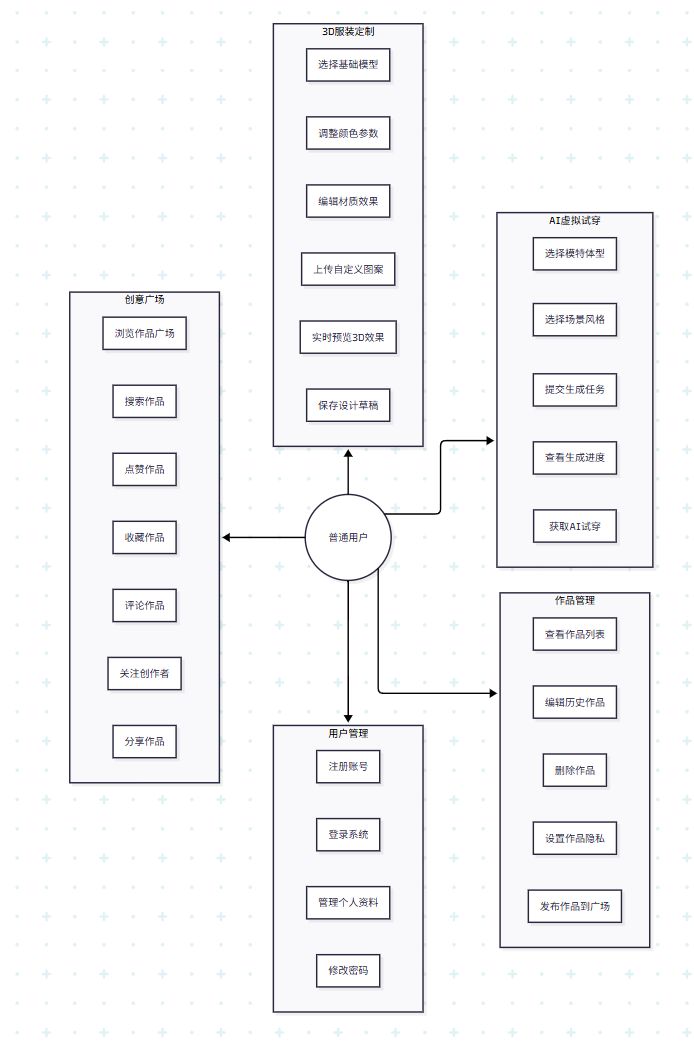
\includegraphics[width=0.85\textwidth]{useCase1.png}
	\caption{普通用户用例图}
	\label{fig:usecase-user}
\end{figure}

为便于后续模块设计与接口实现，选取普通用户中的关键用例进行用例规约编写，规约内容包含前置条件、基本流程、异常处理与后置条件等要素，用于明确业务边界与异常场景，如表~\ref{tab:usecase-user} 所示。

\begin{table}[H]
	\centering
	\caption{普通用户关键用例规约}
	\label{tab:usecase-user}
	\renewcommand{\arraystretch}{1.25}
	\setlength{\tabcolsep}{0.2ex}
	\begin{tabular}{@{}>{\raggedright\arraybackslash}p{0.11\textwidth} >{\raggedright\arraybackslash}p{0.14\textwidth} >{\raggedright\arraybackslash}p{0.12\textwidth} >{\raggedright\arraybackslash}p{0.255\textwidth} >{\raggedright\arraybackslash}p{0.245\textwidth} >{\raggedright\arraybackslash}p{0.11\textwidth}@{}}
		\toprule
		\mbox{用例编号} & \mbox{用例名称} & \mbox{前置条件} & \mbox{基本流程} & \mbox{扩展流程} & \mbox{后置条件} \\
		\midrule
		UC01 & 用户注册/登录 & 用户未登录 &
		1.~输入账号密码\newline 2.~系统校验\newline 3.~登录成功进入系统 &
		1.~账号或密码错误\newline 2.~提示重新输入 &
		用户成功登录系统 \\
		UC02 & 浏览创意广场 & 用户已登录 &
		1.~进入创意广场\newline 2.~系统加载作品列表\newline 3.~用户浏览作品 &
		1.~数据加载失败\newline 2.~提示刷新 &
		成功展示作品列表 \\
		UC03 & 3D 服装定制 & 已选择服装模型 &
		1.~选择模型\newline 2.~调整颜色/材质/图案\newline 3.~实时预览效果 &
		1.~模型加载失败\newline 2.~参数异常 &
		生成个性化 3D 设计 \\
		UC04 & AI 虚拟试穿 & 已完成 3D 设计 &
		1.~点击生成试穿\newline 2.~调用 AI 接口\newline 3.~返回试穿图 &
		1.~AI 生成失败\newline 2.~网络异常 &
		成功生成试穿图 \\
		UC05 & 发布作品 & 已生成设计作品 &
		1.~填写作品信息\newline 2.~提交发布\newline 3.~系统保存作品 &
		1.~提交失败\newline 2.~信息不完整 &
		作品成功发布 \\
		UC06 & 点赞/评论/收藏 & 浏览作品中 &
		1.~点击点赞/评论/收藏\newline 2.~系统记录行为 &
		1.~操作失败\newline 2.~网络异常 &
		互动数据更新 \\
		UC07 & 个人作品管理 & 用户已登录 &
		1.~查看个人作品\newline 2.~编辑或删除作品 &
		1.~操作失败\newline 2.~权限异常 &
		作品被成功管理 \\
		\bottomrule
	\end{tabular}
\end{table}

\subsection{系统管理员}

系统管理员负责平台的日常运营和维护，包括用户管理、内容审核、作品管理和模型库维护。

系统管理员主要承担平台治理与资源维护职责：一方面对用户账号进行管理，保障平台安全与秩序；另一方面对用户提交的作品进行审核与发布控制，确保内容合规；同时维护模型库、材质库以及分类等基础资源，为前端创作与展示提供稳定的数据支撑。系统管理员用例图如图~\ref{fig:usecase-admin} 所示。

\begin{figure}[H]
	\centering
	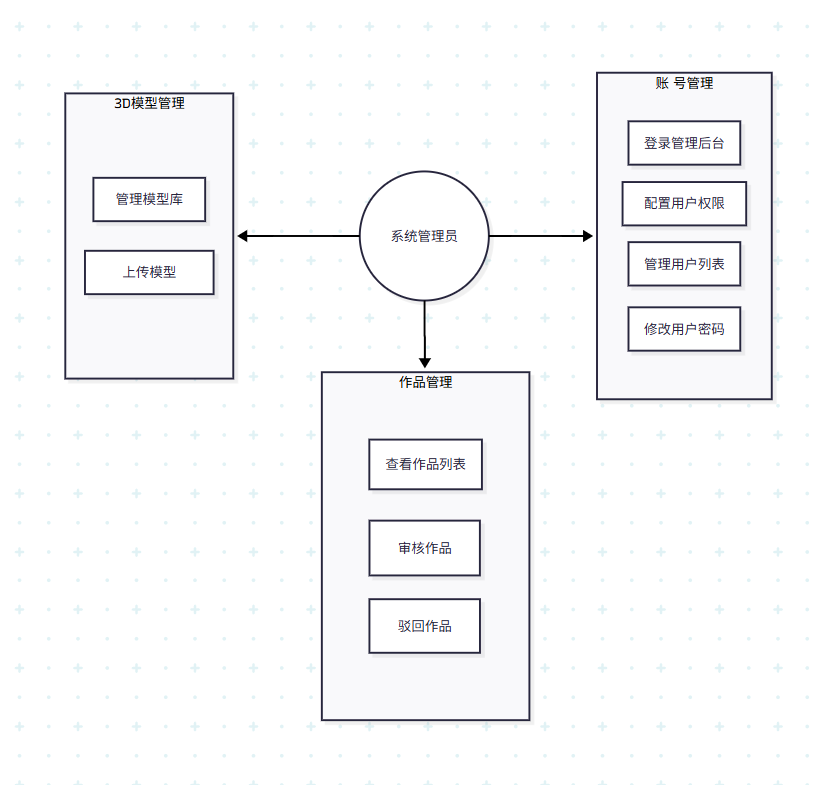
\includegraphics[width=0.85\textwidth]{useCase2.png}
	\caption{系统管理员用例图}
	\label{fig:usecase-admin}
\end{figure}

进一步选取系统管理员侧的关键用例进行规约编写，覆盖登录鉴权、用户管理、作品审核、模型/材质资源维护以及分类与内容管理等核心操作，为后台管理模块的页面功能拆分、权限控制策略与数据一致性处理提供依据，如表~\ref{tab:usecase-admin} 所示。

\begin{table}[H]
	\centering
	\caption{系统管理员关键用例规约}
	\label{tab:usecase-admin}
	\renewcommand{\arraystretch}{1.25}
	\setlength{\tabcolsep}{0.2ex}
	\begin{tabular}{@{}>{\raggedright\arraybackslash}p{0.11\textwidth} >{\raggedright\arraybackslash}p{0.15\textwidth} >{\raggedright\arraybackslash}p{0.13\textwidth} >{\raggedright\arraybackslash}p{0.245\textwidth} >{\raggedright\arraybackslash}p{0.235\textwidth} >{\raggedright\arraybackslash}p{0.11\textwidth}@{}}
		\toprule
		\mbox{用例编号} & \mbox{用例名称} & \mbox{前置条件} & \mbox{基本流程} & \mbox{扩展流程} & \mbox{后置条件} \\
		\midrule
		AC01 & 管理员登录 & 管理员账号存在 &
		1.~输入账号密码\newline 2.~系统校验\newline 3.~登录后台 &
		1.~登录失败\newline 2.~权限不足 &
		成功进入管理后台 \\
		AC02 & 用户管理 & 已登录后台 &
		1.~查看用户列表\newline 2.~编辑/禁用用户 &
		1.~操作失败\newline 2.~用户不存在 &
		用户信息更新 \\
		AC03 & 作品审核 & 存在待审核作品 &
		1.~查看作品\newline 2.~审核通过或拒绝 &
		1.~审核失败\newline 2.~数据异常 &
		审核结果生效 \\
		AC04 & 模型库管理 & 已登录后台 &
		1.~上传模型\newline 2.~修改/删除模型 &
		1.~上传失败\newline 2.~格式错误 &
		模型库更新 \\
		AC05 & 材质库管理 & 已登录后台 &
		1.~上传材质\newline 2.~编辑/删除材质 &
		1.~操作失败\newline 2.~文件异常 &
		材质库更新 \\
		AC06 & 分类与内容管理 & 已登录后台 &
		1.~新增分类\newline 2.~修改/删除分类 &
		1.~操作失败 &
		分类信息更新 \\
		\bottomrule
	\end{tabular}
\end{table}

\section{主要功能需求}

\begin{enumerate}[label=(\arabic*)]
	\item \textbf{用户管理模块}：支持用户注册、登录、个人信息管理功能。系统采用 JWT 认证机制，区分普通用户和管理员两种角色。普通用户可管理个人作品、参与社区互动；管理员拥有内容审核、用户管理和 3D 模型管理权限。
	\item \textbf{3D 服装定制模块}：提供基于 Web3D 的服装可视化编辑工具。用户可选择基础服装模型，实时调整颜色、材质参数，上传自定义图案并指定应用部位，通过鼠标交互旋转、缩放查看模型细节。系统需保证渲染流畅性，编辑操作响应延迟控制在 100\,ms 以内。
	\item \textbf{AI 虚拟试穿模块}：支持将定制完成的 3D 服装转换为真人试穿图像。用户选择模特体型和场景风格后，系统调用 AI 服务生成高保真效果图。该模块需处理任务队列管理、生成进度反馈和结果展示功能，平均生成耗时控制在 30 秒以内。
	\item \textbf{创意广场模块}：提供作品发布、浏览、搜索功能。支持按热度、时间、标签等排序，实现点赞、收藏、评论等互动操作。用户可关注其他创作者，便于查看喜欢的作品类型。
	\item \textbf{作品管理模块}：支持用户对 3D 草稿和 AI 成图的完整生命周期管理，包括保存、编辑、删除、提审、发布设置。提供作品历史版本回溯功能。
	\item \textbf{后台管理模块}：管理员可进行用户账号状态管理、作品内容审核、3D 模型库维护等操作。
\end{enumerate}

\section{系统数据需求}

\subsection{数据流图}

根据系统功能需求分析，画出主要功能的数据流图。系统的数据流图如图~\ref{fig:dataflow} 所示。

图中外部实体包括普通用户、管理员以及对象存储/文件服务；系统内部处理过程主要由用户认证与资料（P1）、作品管理（P2）、版本管理/参数提交（P3）、文件/模型资源管理（P6）、审核管理（P4）与创意广场互动（P5）组成。普通用户完成登录后，可创建作品并上传模型文件，文件服务返回的 URL 与元数据写入 \texttt{model\_files} 并关联 \texttt{design\_works}；版本与参数写入 \texttt{design\_versions}。作品/版本提审后进入审核流程，管理员在 P4 中审核并将结果记录到 \texttt{design\_reviews}，同时回写更新 \texttt{design\_works} 的状态与发布信息。作品发布后，创意广场产生点赞、收藏、评论与标签等互动，分别写入 \texttt{work\_likes}、\texttt{work\_favorites}、\texttt{work\_comments} 和 \texttt{work\_tags}，并更新作品热度计数。

\begin{figure}[H]
	\centering
	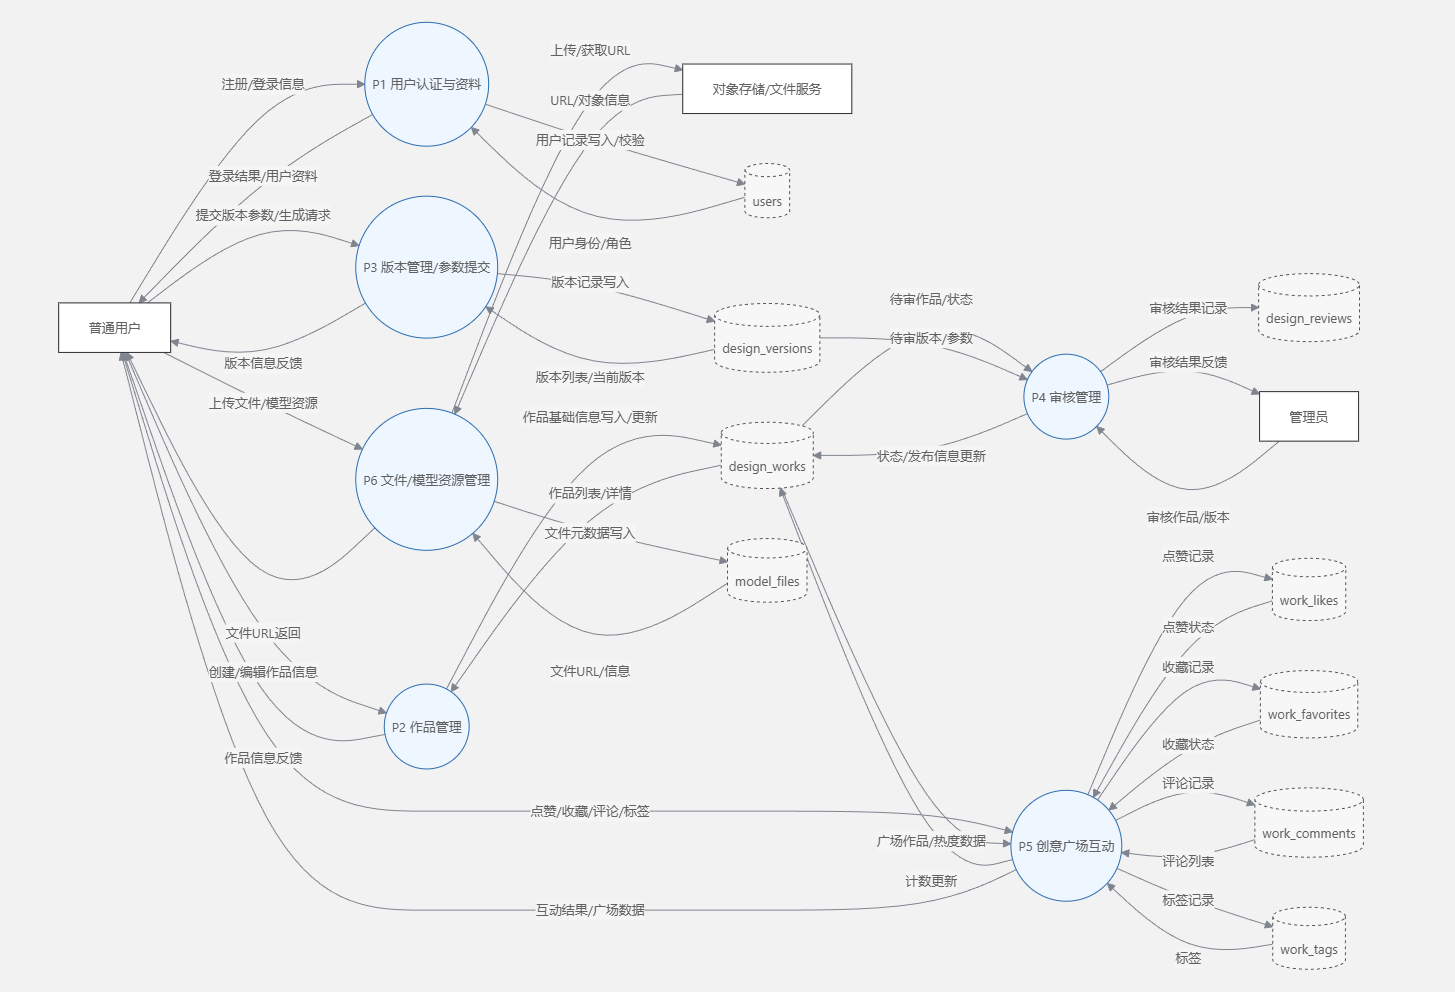
\includegraphics[width=0.88\textwidth]{dataFlow.png}
	\caption{系统数据流图}
	\label{fig:dataflow}
\end{figure}

\subsection{数据项}

根据数据流图以及数据流的描述，可以得到数据库设计所需数据项。系统的数据库设计所需的各数据项描述如表~\ref{tab:dataitems} 所示。

\renewcommand{\arraystretch}{1.3}

{
\small % 控制整体字体（关键）

\begin{longtable}{
>{\RaggedRight\arraybackslash}p{0.12\textwidth}
>{\RaggedRight\arraybackslash}p{0.18\textwidth}
>{\RaggedRight\arraybackslash}p{0.14\textwidth}
>{\RaggedRight\arraybackslash}p{0.16\textwidth}
>{\centering\arraybackslash}p{0.08\textwidth}
>{\RaggedRight\arraybackslash}p{0.22\textwidth}
}

\caption{系统数据库设计数据项}\label{tab:dataitems} \\
\toprule
数据项名 & 数据项含义 & 别名 & 数据类型 & 长度 & 取值范围 \\
\midrule
\endfirsthead

\multicolumn{6}{c}{\zihao{5}续表\thetable\quad 系统数据库设计数据项表}\\
\toprule
数据项名 & 数据项含义 & 别名 & 数据类型 & 长度 & 取值范围 \\
\midrule
\endhead

\bottomrule
\endfoot

\bottomrule
\endlastfoot

id & 主键 ID & user\_\allowbreak id & bigint unsigned & 20 & $\ge 1$，自增 \\ username & 登录用户名（唯一） & login\_\allowbreak name & varchar & 50 & 非空，唯一 \\ password & 加密后的密码 & pwd\_\allowbreak hash & varchar & 255 & 非空 \\ avatar & 头像 URL 地址 & avatar\_\allowbreak url & varchar & 255 & 为空或合法 URL \\ role & 角色权限：1 普通用户，2 管理员 & user\_\allowbreak role & tinyint unsigned & 2 & \{1,2\} \\ created\_\allowbreak at & 注册时间 & register\_\allowbreak time & datetime & - & 合法时间 \\ updated\_\allowbreak at & 最后更新时间 & update\_\allowbreak time & datetime & - & 合法时间 \\ id & 主键 ID & file\_\allowbreak id & bigint unsigned & 20 & $\ge 1$，自增 \\ name & 展示名称 & file\_\allowbreak name & varchar & 255 & 非空 \\ url & 访问 URL & file\_\allowbreak url & varchar & 1024 & 非空，合法 URL \\ size & 文件大小（byte） & file\_\allowbreak size & bigint unsigned & 20 & $\ge 0$ \\ created\_\allowbreak at & 创建时间 & create\_\allowbreak time & datetime & - & 合法时间 \\ updated\_\allowbreak at & 更新时间 & update\_\allowbreak time & datetime & - & 合法时间 \\ id & 主键 ID & work\_\allowbreak id & bigint unsigned & 20 & $\ge 1$，自增 \\ user\_\allowbreak id & 作者用户 ID & author\_\allowbreak id & bigint unsigned & 20 & $\ge 1$ \\ title & 作品标题 & work\_\allowbreak title & varchar & 255 & 非空 \\ description & 作品描述 & work\_\allowbreak desc & text & - & 可为空 \\ cover\_\allowbreak file\_\allowbreak id & 封面文件 ID & cover\_\allowbreak id & bigint unsigned & 20 & 可为空或 $\ge 1$ \\ status & 作品状态 & work\_\allowbreak status & tinyint unsigned & 3 & $\ge 0$（按业务定义状态码） \\ published\_\allowbreak at & 发布时间 & publish\_\allowbreak time & datetime & - & 可为空或合法时间 \\ created\_\allowbreak at & 创建时间 & create\_\allowbreak time & datetime & - & 合法时间 \\ updated\_\allowbreak at & 更新时间 & update\_\allowbreak time & datetime & - & 合法时间 \\ likes\_\allowbreak count & 点赞数 & like\_\allowbreak cnt & int & - & $\ge 0$ \\ comments\_\allowbreak count & 评论数 & comment\_\allowbreak cnt & int & - & $\ge 0$ \\ favorites\_\allowbreak count & 收藏数 & fav\_\allowbreak cnt & int & - & $\ge 0$ \\ is\_\allowbreak featured & 是否精选 & featured\_\allowbreak flag & tinyint & 1 & \{0,1\} \\ id & 主键 ID & review\_\allowbreak id & bigint unsigned & 20 & $\ge 1$，自增 \\ work\_\allowbreak id & 作品 ID & work\_\allowbreak id & bigint unsigned & 20 & $\ge 1$ \\ admin\_\allowbreak id & 审核管理员 ID & reviewer\_\allowbreak id & bigint unsigned & 20 & $\ge 1$ \\ result & 审核结果码 & review\_\allowbreak result & tinyint unsigned & 3 & $\ge 0$（按业务定义结果码） \\ reason & 审核原因/说明 & review\_\allowbreak reason & varchar & 1024 & 可为空或字符串 \\ reviewed\_\allowbreak at & 审核时间 & review\_\allowbreak time & datetime & - & 合法时间 \\ id & 主键 ID & tag\_\allowbreak id & bigint unsigned & 20 & $\ge 1$，自增 \\ work\_\allowbreak id & 作品 ID & work\_\allowbreak id & bigint unsigned & 20 & $\ge 1$ \\ tag & 标签内容 & tag\_\allowbreak name & varchar & 32 & 非空 \\ id & 主键 ID & like\_\allowbreak id & bigint unsigned & 20 & $\ge 1$，自增 \\ work\_\allowbreak id & 作品 ID & work\_\allowbreak id & bigint unsigned & 20 & $\ge 1$ \\ user\_\allowbreak id & 点赞用户 ID & user\_\allowbreak id & bigint unsigned & 20 & $\ge 1$ \\ created\_\allowbreak at & 点赞时间 & like\_\allowbreak time & datetime & - & 合法时间 \\ id & 主键 ID & fav\_\allowbreak id & bigint unsigned & 20 & $\ge 1$，自增 \\ work\_\allowbreak id & 作品 ID & work\_\allowbreak id & bigint unsigned & 20 & $\ge 1$ \\ user\_\allowbreak id & 收藏用户 ID & user\_\allowbreak id & bigint unsigned & 20 & $\ge 1$ \\ created\_\allowbreak at & 收藏时间 & fav\_\allowbreak time & datetime & - & 合法时间 \\ id & 主键 ID & comment\_\allowbreak id & bigint unsigned & 20 & $\ge 1$，自增 \\ work\_\allowbreak id & 作品 ID & work\_\allowbreak id & bigint unsigned & 20 & $\ge 1$ \\ user\_\allowbreak id & 评论用户 ID & user\_\allowbreak id & bigint unsigned & 20 & $\ge 1$ \\ content & 评论内容 & comment\_\allowbreak text & text & - & 非空 \\ created\_\allowbreak at & 评论时间 & comment\_\allowbreak time & datetime & - & 合法时间 \\
\end{longtable}
}

\chapter{系统设计}%

\section{系统总体设计}

\subsection{系统架构设计}

本平台面向普通用户与系统管理员两类角色，围绕“3D 服装可视化定制”和“AI 真人试穿效果生成”构建“工具 + 社区”的一体化应用形态，系统采用“前端—后端—数据层—外部 AI 服务”的分层架构（见图~\ref{fig:systemArchitecture}）。其中，前端聚焦三维渲染与交互，将复杂的服装编辑过程以参数化方式呈现并实时预览，降低创作门槛；后端统一承载鉴权与业务规则，对作品、版本与互动等数据进行一致性管理，并以标准接口向前端返回业务数据；通过任务化/异步化方式接入AI 试穿，由后端负责创建任务、维护状态与结果回写；数据层将结构化业务数据与大文件资源存储至云端，以url形式保存，并引入缓存与队列机制提升热点访问与任务处理效率，从而支撑平台的稳定运行与后续功能扩展。

\begin{figure}[H]
	\centering
	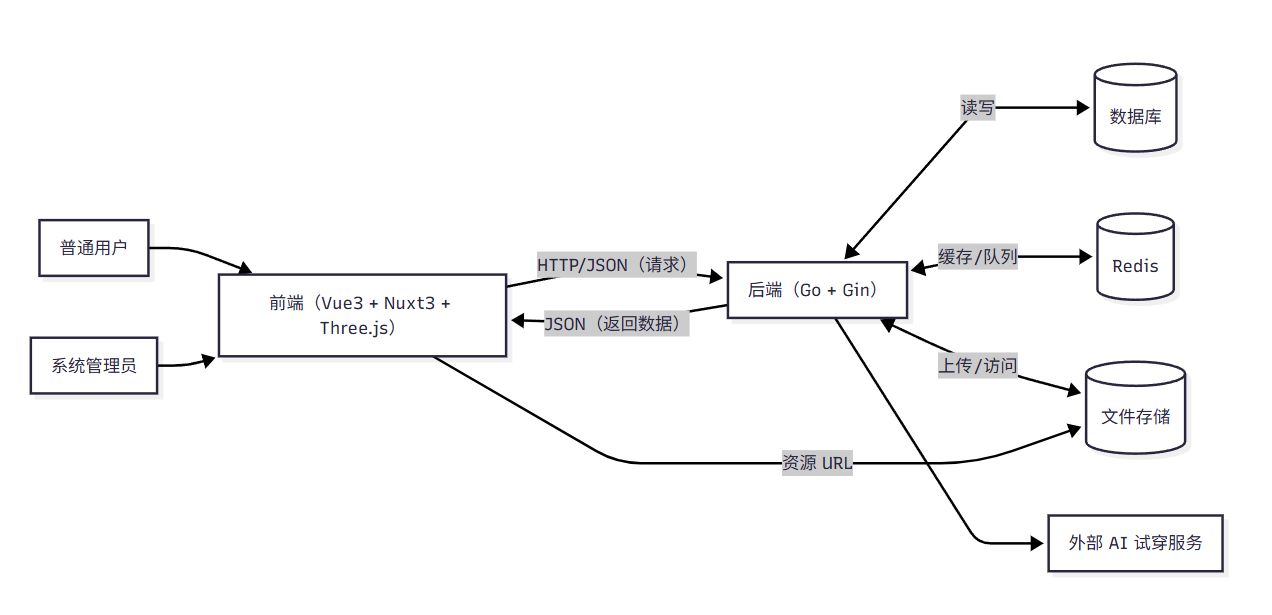
\includegraphics[width=0.88\textwidth]{systemArchitecture.png}
	\caption{系统架构图}
	\label{fig:systemArchitecture}
\end{figure}

\subsection{系统功能结构设计}

系统功能结构采用“角色—业务域—功能点”的划分方式，保证前台创作与社区能力、后台治理能力相互独立又可协同。系统总体功能结构如图~\ref{fig:functionStructure} 所示。

\begin{figure}[H]
	\centering
	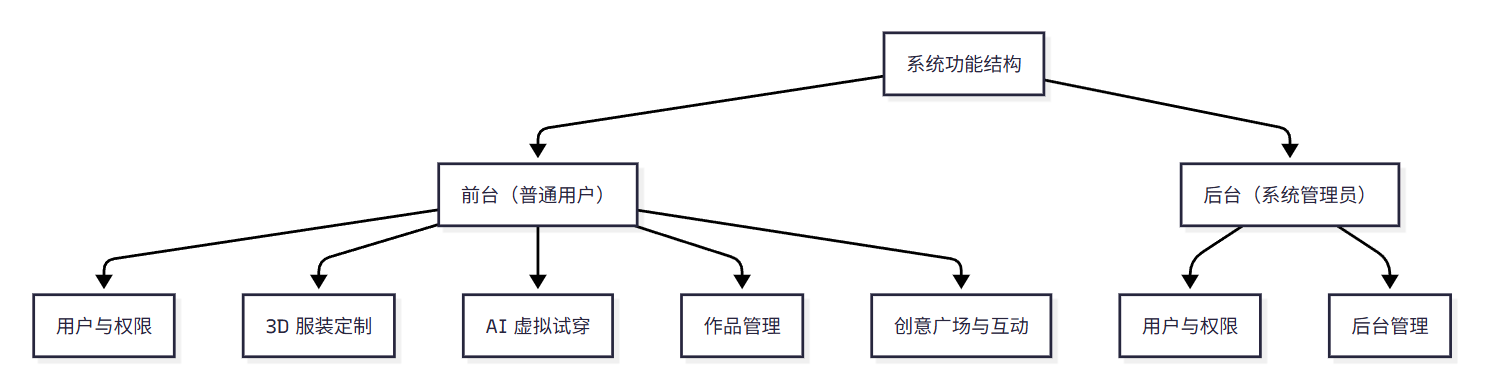
\includegraphics[width=0.95\textwidth]{Power.png}
	\caption{系统功能结构图}
	\label{fig:functionStructure}
\end{figure}

整体功能结构如下：
\subsubsection*{（1）用户与权限}
注册登录、JWT 鉴权、角色区分（普通用户/管理员）、个人信息维护。

\subsubsection*{（2）3D 服装定制}
基础模型选择、颜色与材质参数调整、图案上传与部位应用、三维交互（旋转/缩放/查看细节）、设计草稿保存。

\subsubsection*{（3）AI 虚拟试穿}
模特体型/场景风格选择、生成任务创建、生成进度反馈、结果展示与保存。

\subsubsection*{（4）作品管理}
作品信息编辑、草稿、发布/下架/删除、编辑回溯。

\subsubsection*{（5）创意广场与互动}
作品浏览/搜索/排序（热度/时间/标签）、点赞/收藏/评论、关注创作者、个人作品主页展示。

\subsubsection*{（6）后台管理}
管理员登录、用户管理、作品审核（通过/拒绝/下架）、模型库维护。

\section{系统功能模块设计}

系统功能模块设计以“前台创作与社区 + 后台治理运营”为主线，围绕用户体系、3D 定制、AI 试穿、作品管理、创意广场互动与后台管理等核心业务模块展开。各模块之间以统一的后端接口进行解耦协作，以“作品/分享”为核心业务对象贯通数据，形成完整的创作与运营闭环。

\begingroup
% 说明：本章节图较多，为避免 samepage + [H] 造成大段留白，
% 采用更灵活的浮动策略，并适当收紧图文间距（仅在本章节生效）。
\setlength{\textfloatsep}{10pt plus 2pt minus 2pt}
\setlength{\intextsep}{10pt plus 2pt minus 2pt}
\setlength{\abovecaptionskip}{6pt}
\setlength{\belowcaptionskip}{0pt}

\subsection{用户与权限模块}

模块功能：该模块为系统提供身份认证与权限控制能力，覆盖用户注册、登录、退出、个人信息维护与角色权限校验等功能。系统采用 JWT 作为鉴权载体，在保证前端无状态访问的同时，实现普通用户与管理员接口的权限隔离，为作品发布、互动与后台治理提供统一的安全入口。模块功能结构图如图~\ref{fig:userModule}，模块流程图如图~\ref{fig:userModuleFlow} 所示。

\begin{figure}[H]
	\centering
	\begin{minipage}[t]{0.58\textwidth}
		\centering
		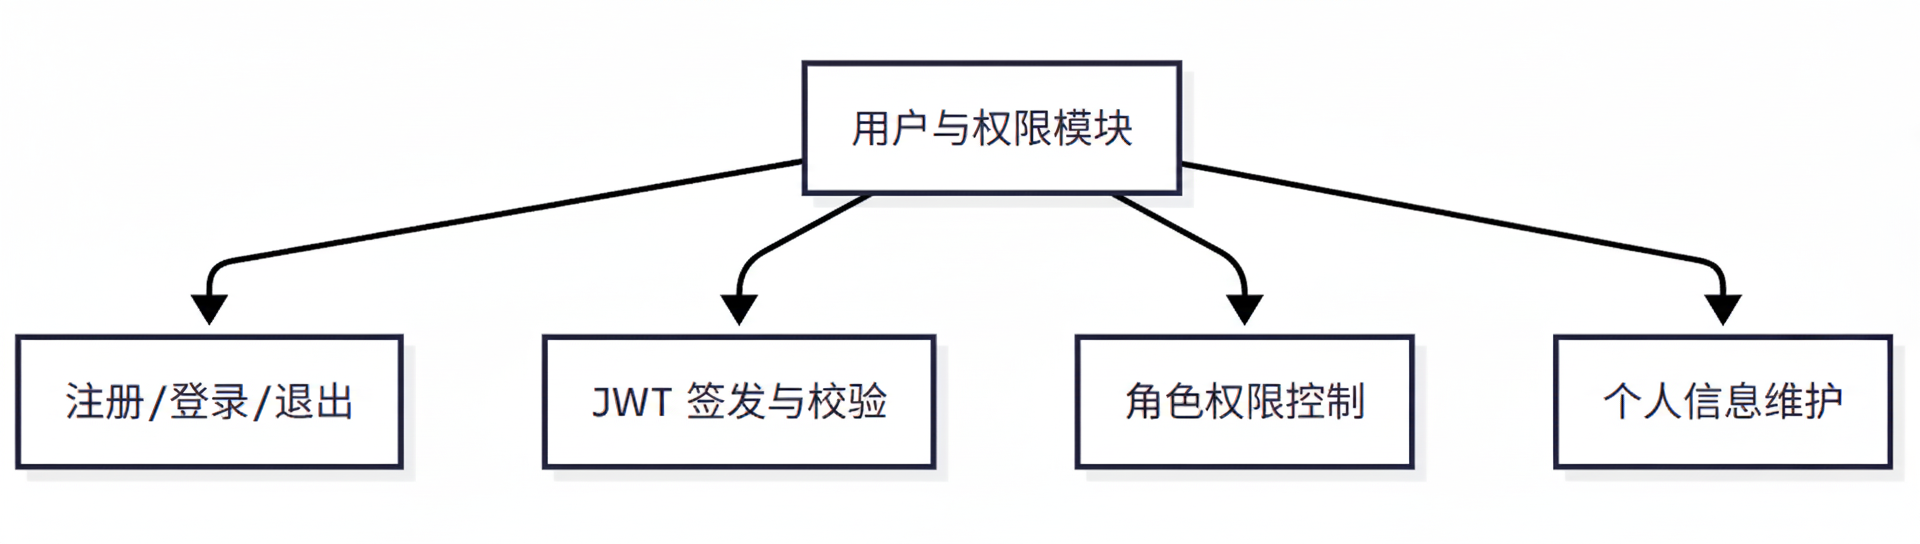
\includegraphics[width=\linewidth]{userModule.png}
		\caption{用户与权限模块功能结构}
		\label{fig:userModule}
	\end{minipage}
	\hfill
	\begin{minipage}[t]{0.38\textwidth}
		\centering
		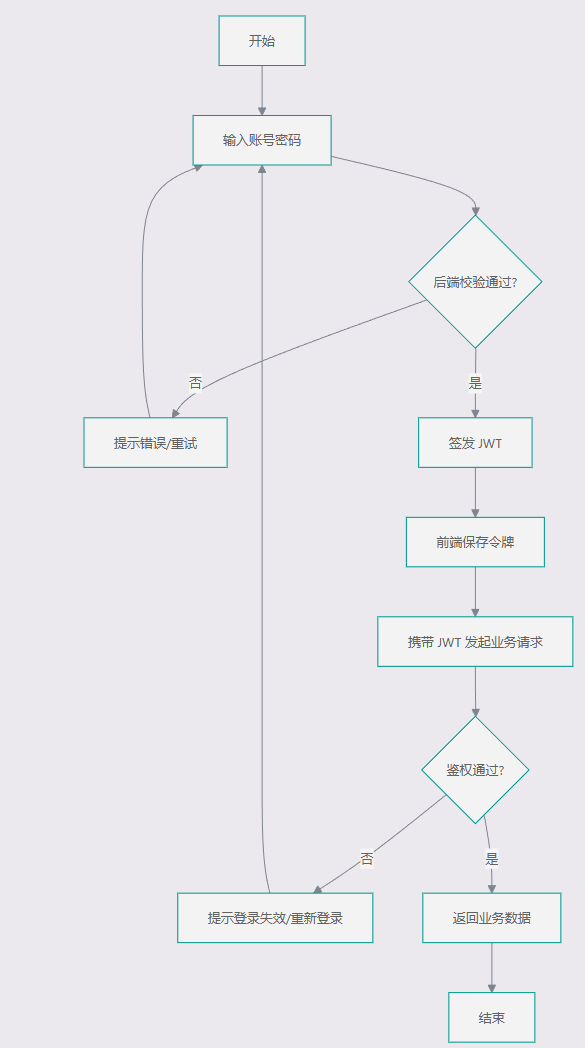
\includegraphics[width=\linewidth]{userModuleFlow.png}
		\caption{用户流程图}
		\label{fig:userModuleFlow}
	\end{minipage}
\end{figure}

模块流程描述：用户提交账号密码完成登录后，后端校验凭证并签发 JWT；前端在后续请求中携带令牌，后端完成令牌校验与角色鉴权后返回业务数据；当用户退出或令牌失效时，前端清理本地令牌并重新进入登录流程。

\subsection{3D 服装定制模块}

模块功能：该模块在浏览器端提供三维可视化服装定制能力，支持基础模型选择、颜色与材质参数调整、图案上传与部位应用、视角控制与细节预览等操作。服装三维捕获与重定向技术\cite{pons2017clothcap}的研究成果为本模块的服装形变处理提供了参考基础。用户可将定制配置保存为草稿或作品版本，为作品发布提供可复用的设计数据。模块功能结构图如图~\ref{fig:3dModule}，模块流程图如图~\ref{fig:3dModuleFlow} 所示。

\begin{figure}[H]
	\centering
	\begin{minipage}[t]{0.58\textwidth}
		\centering
		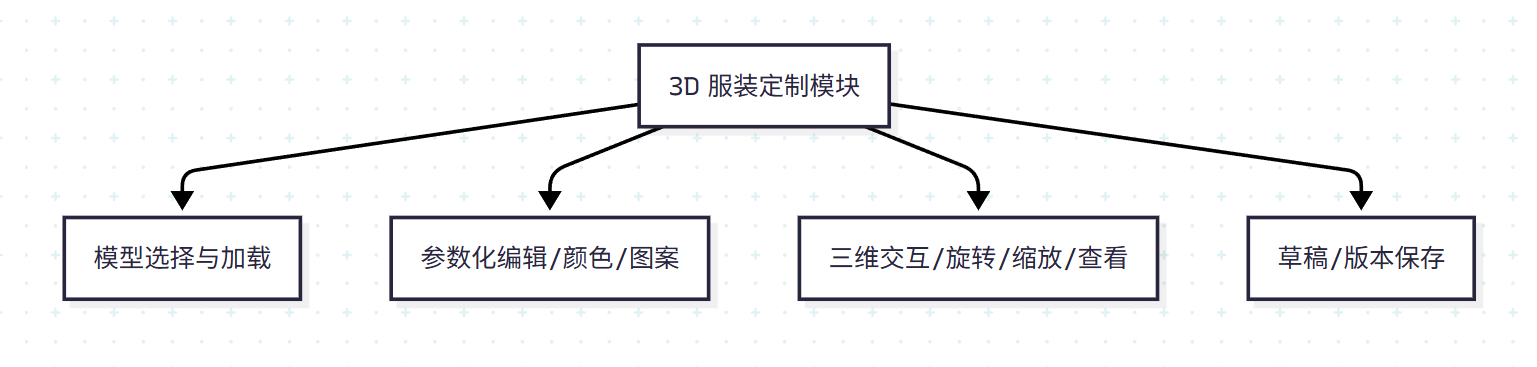
\includegraphics[width=\linewidth]{3dModule.png}
		\caption{3D 服装定制模块功能结构}
		\label{fig:3dModule}
	\end{minipage}
	\hfill
	\begin{minipage}[t]{0.38\textwidth}
		\centering
		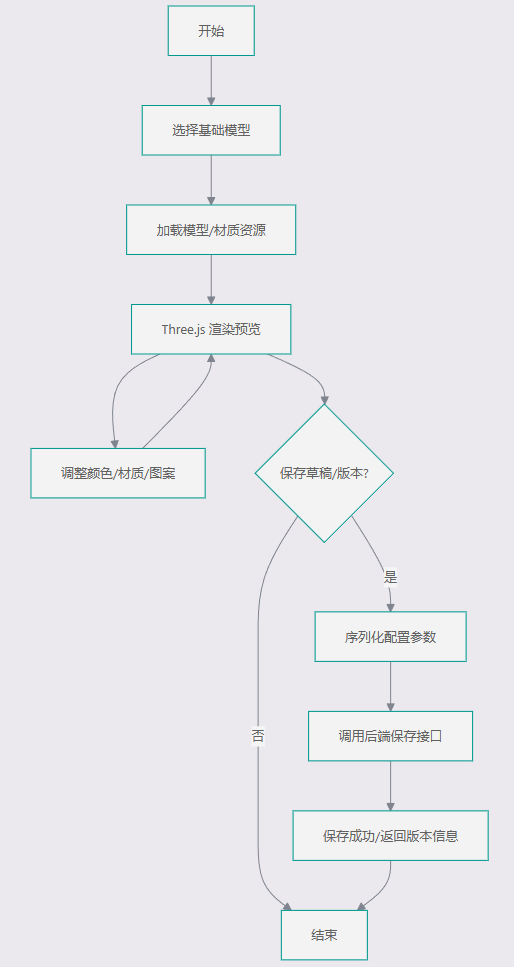
\includegraphics[width=\linewidth]{3dModuleFlow.png}
		\caption{3D 服装定制模块流程图}
		\label{fig:3dModuleFlow}
	\end{minipage}
\end{figure}

模块流程描述：用户选择服装类型后，前端加载模型与材质资源并渲染；用户通过交互面板调整参数并实时预览；当用户保存时，前端将关键配置参数（模型引用、材质与贴图、颜色与部位信息等）提交至后端形成草稿/版本记录，支持后续继续编辑或提审发布。

\subsection{AI 虚拟试穿模块}

模块功能：该模块将用户的 3D 设计各角度平面图作为条件输入，生成高保真的真人试穿效果图。本系统 AI 试穿功能以去噪扩散概率模型（DDPM）\cite{ddpm_ho2020}为核心基础，借助潜在扩散模型（LDM）\cite{ldm_rombach2022}的高效图像合成能力，并采用 ControlNet\cite{controlnet_zhang2023} 实现以 3D 服装渲染图为控制条件的引导生成。试穿前处理流程中涉及人体姿态估计\cite{cao2021openpose}与人体语义解析\cite{li2022schp}，以保证服装与人体的对齐精度。最终参考 M3D-VTON\cite{m3d_vton}的单目转三维方案提升试穿立体感。由于 AI 生成属于耗时任务，系统采用任务化/异步化机制：后端创建任务并返回任务 ID，任务执行模块从队列取出任务调用外部 AI 服务，生成结果保存至文件存储并写入数据库，前端通过查询接口获取进度并展示结果。模块功能结构图如图~\ref{fig:aiModule}，模块流程图如图~\ref{fig:aiModuleFlow} 所示。

\begin{figure}[H]
	\centering
	\begin{minipage}[t]{0.55\textwidth}
		\centering
		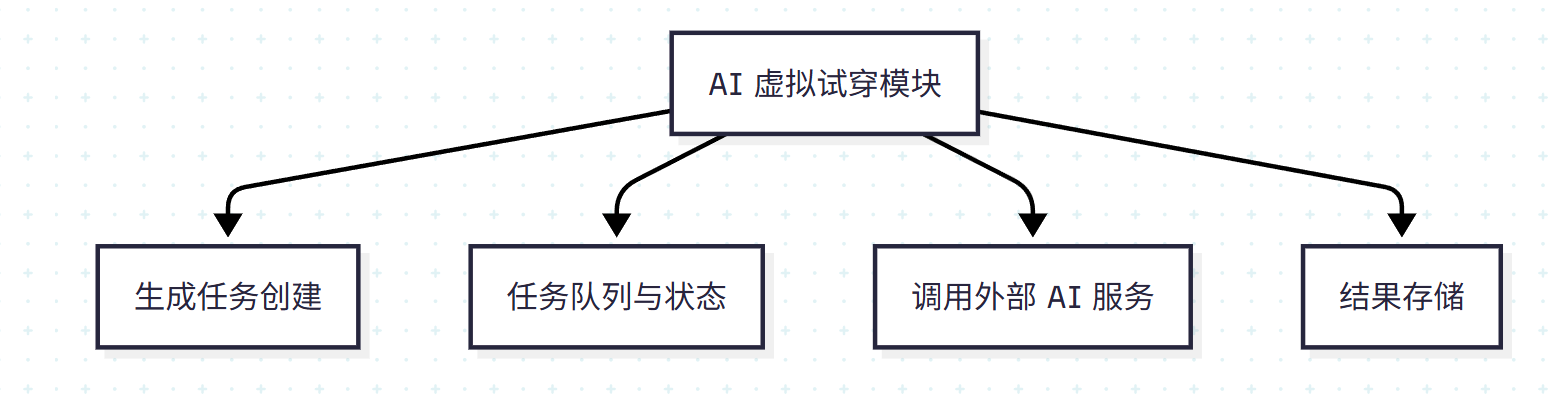
\includegraphics[width=\linewidth]{aiModule.png}
		\caption{AI 虚拟试穿模块功能结构}
		\label{fig:aiModule}
	\end{minipage}
	\hfill
	\begin{minipage}[t]{0.41\textwidth}
		\centering
		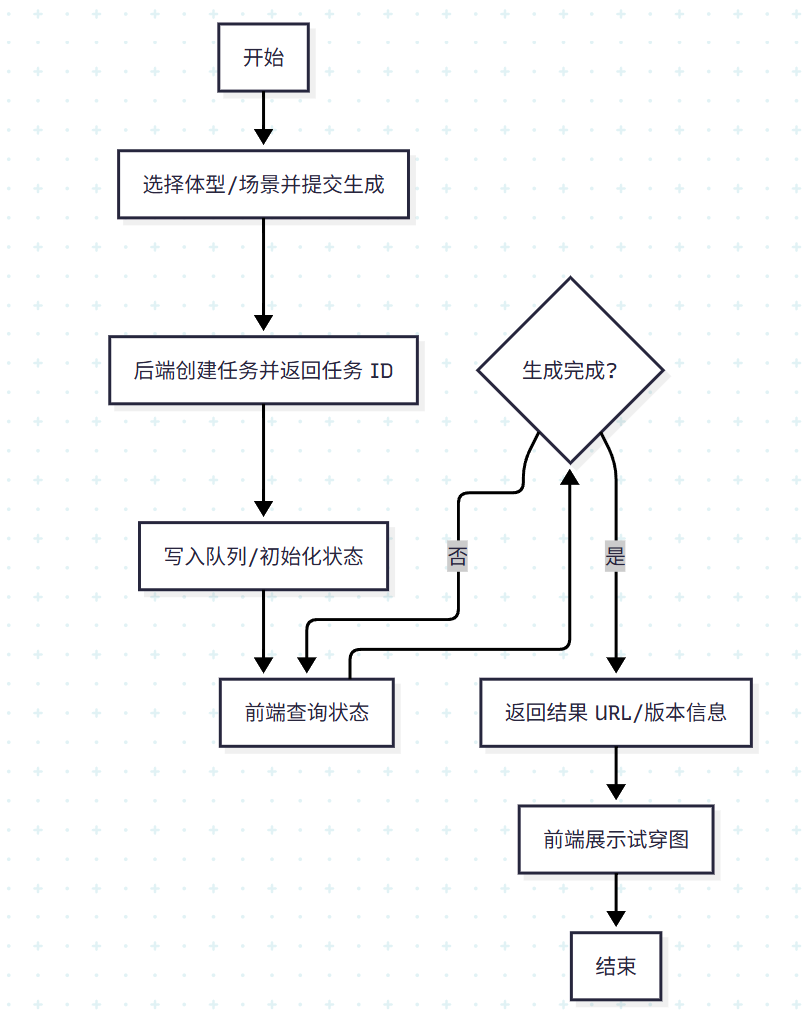
\includegraphics[width=\linewidth]{aiModuleFlow.png}
		\caption{AI 虚拟试穿模块流程图}
		\label{fig:aiModuleFlow}
	\end{minipage}
\end{figure}

模块流程描述：用户在前端选择模特与场景风格后提交生成请求；后端创建任务写入队列并返回任务 ID；前端基于任务 ID 查询进度；任务执行模块消费队列调用外部 AI，生成完成后上传结果文件并写入版本数据，更新任务状态；前端获取到完成状态后展示试穿图并允许用户保存。

\subsection{作品管理模块}

模块功能：该模块面向普通用户提供作品全生命周期管理能力，包含作品创建、信息编辑、草稿、发布/下架、删除等功能。模块功能结构图如图~\ref{fig:workModule}，模块流程图如图~\ref{fig:workModuleFlow} 所示。

\begin{figure}[H]
	\centering
	\begin{minipage}[t]{0.56\textwidth}
		\centering
		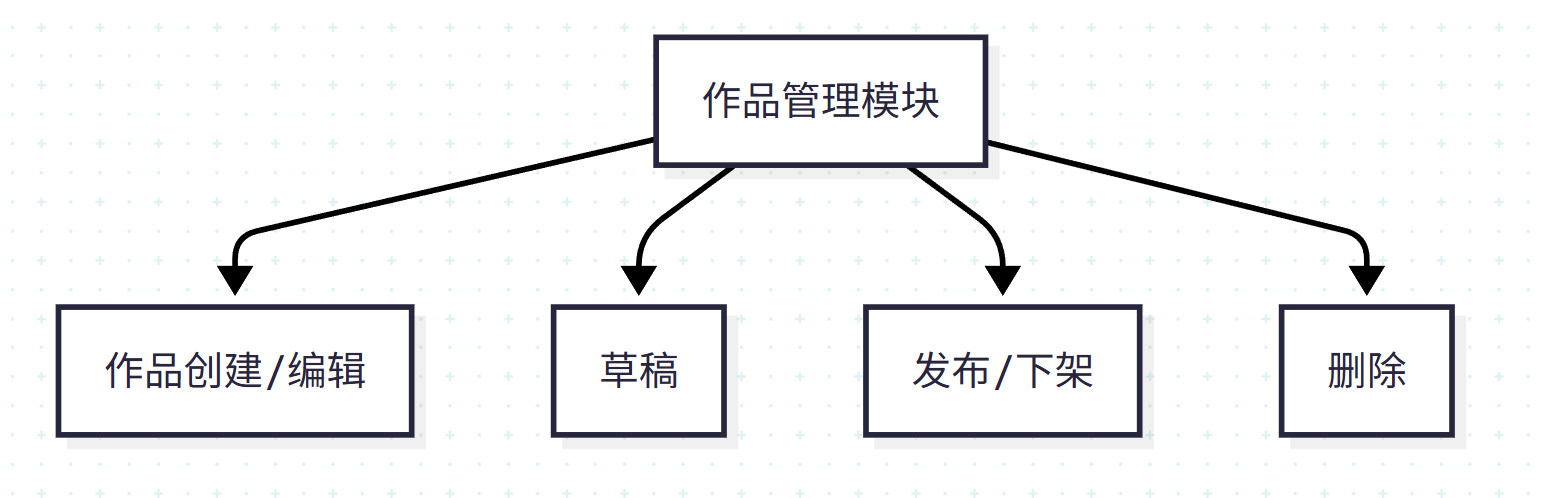
\includegraphics[width=\linewidth]{workModule.png}
		\caption{作品管理模块功能结构}
		\label{fig:workModule}
	\end{minipage}
	\hfill
	\begin{minipage}[t]{0.40\textwidth}
		\centering
		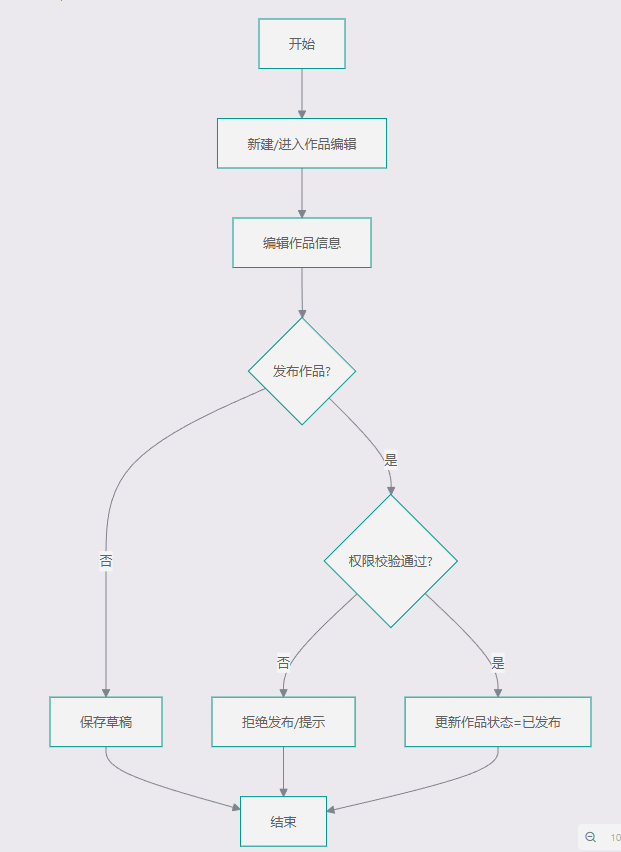
\includegraphics[width=\linewidth]{workModuleFlow.png}
		\caption{作品管理模块流程图}
		\label{fig:workModuleFlow}
	\end{minipage}
\end{figure}

模块流程描述：用户创建作品并编辑标题、描述等信息；编辑完成后存储为草稿可选择提审发布，后端更新作品状态与发布时间；当用户下架或删除作品时，后端校验归属权限并更新状态，保证数据一致性与可审计性。

\subsection{创意广场与社区互动模块}

模块功能：该模块提供作品展示与社区交互能力，包含作品列表浏览、搜索与排序（热度/时间/标签等）、作品详情查看，以及点赞、收藏、评论、关注等互动功能。模块通过将互动行为与作品数据关联，形成反馈闭环，提升作品传播与社区活跃度。模块功能结构图如图~\ref{fig:squareModule}，模块流程图如图~\ref{fig:squareModuleFlow} 所示。

\begin{figure}[H]
	\centering
	\begin{minipage}[t]{0.54\textwidth}
		\centering
		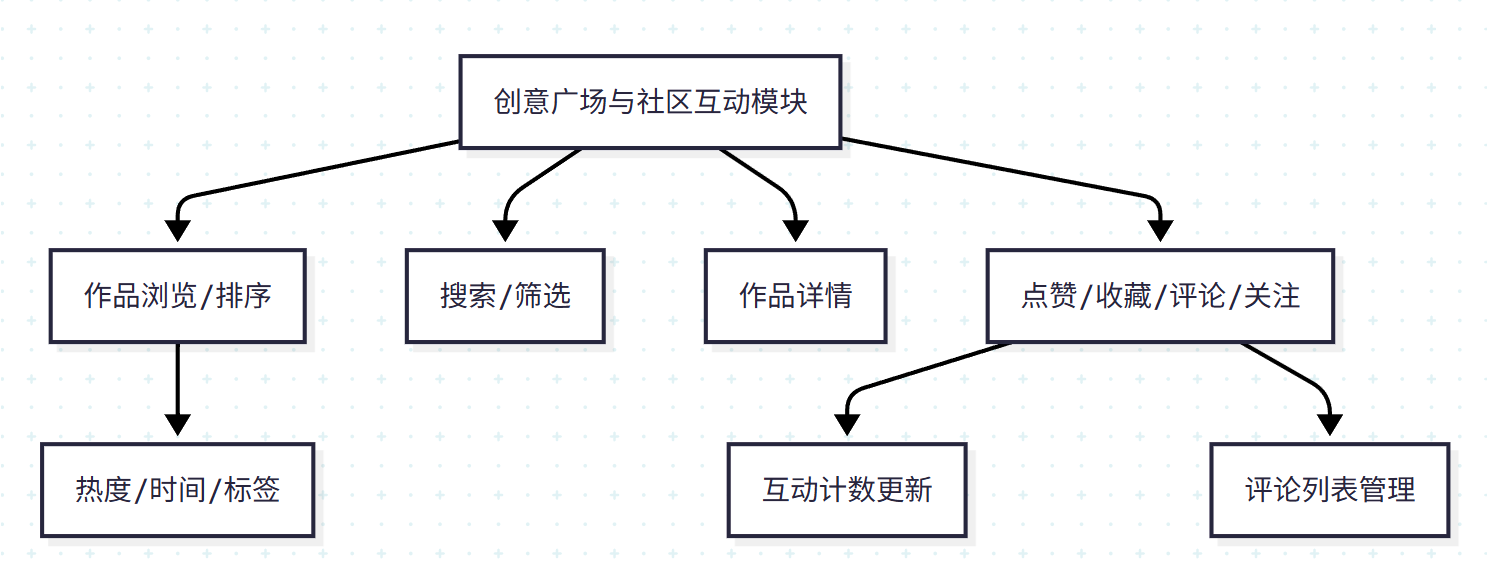
\includegraphics[width=\linewidth]{squareModule.png}
		\caption{创意广场与社区互动模块功能结构}
		\label{fig:squareModule}
	\end{minipage}
	\hfill
	\begin{minipage}[t]{0.42\textwidth}
		\centering
		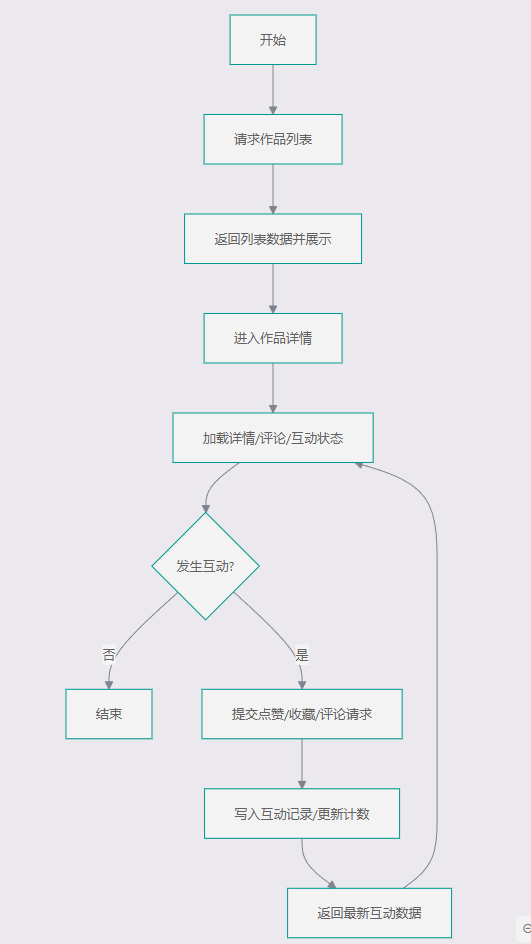
\includegraphics[width=\linewidth]{squareModuleFlow.png}
		\caption{创意广场与社区互动模块流程图}
		\label{fig:squareModuleFlow}
	\end{minipage}
\end{figure}

模块流程描述：用户进入创意广场后，前端请求作品列表并支持排序与筛选；用户打开作品详情页后加载作品信息、互动数据；当用户进行点赞、收藏或评论时，前端提交互动请求，后端校验登录状态并写入互动记录，更新计数并返回最新状态以刷新页面展示。

\subsection{后台管理模块}

模块功能：该模块面向系统管理员提供用户管理、模型管理与内容治理能力，包括用户管理（信息维护，权限分配）、作品内容审核（通过/拒绝/下架）、模型库维护等功能。模块通过权限控制与审核流程保障平台内容质量与资源可用性。模块功能结构图如图~\ref{fig:adminModule}，模块流程图如图~\ref{fig:adminModuleFlow} 所示。

\begin{figure}[H]
	\centering
	\begin{minipage}[t]{0.56\textwidth}
		\centering
		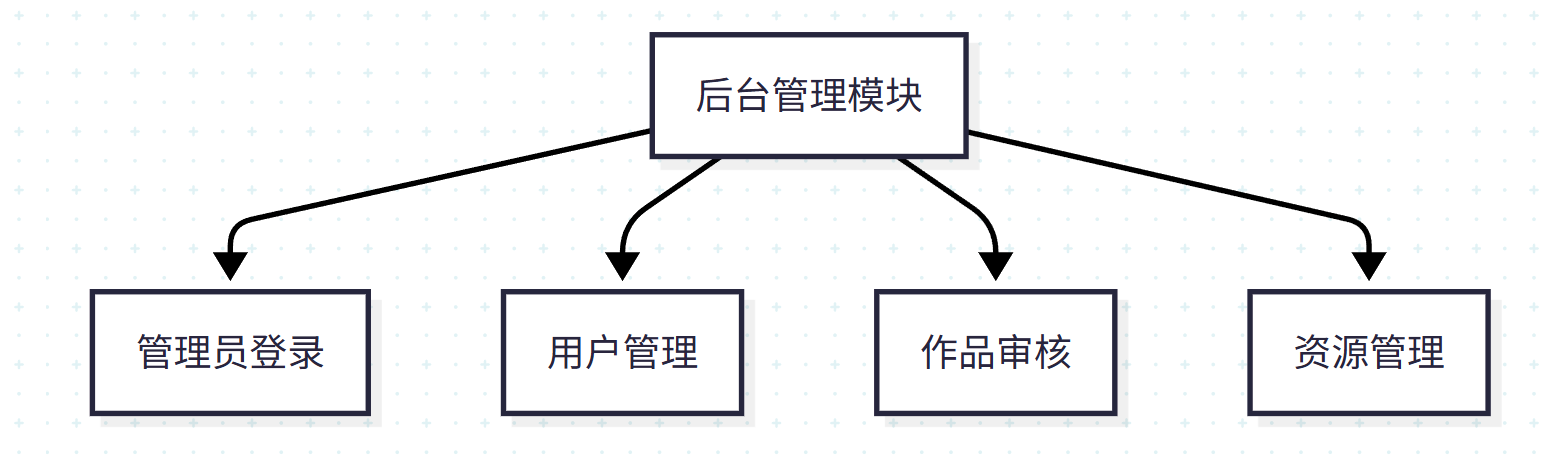
\includegraphics[width=\linewidth]{adminModule.png}
		\caption{后台管理模块功能结构}
		\label{fig:adminModule}
	\end{minipage}
	\hfill
	\begin{minipage}[t]{0.40\textwidth}
		\centering
		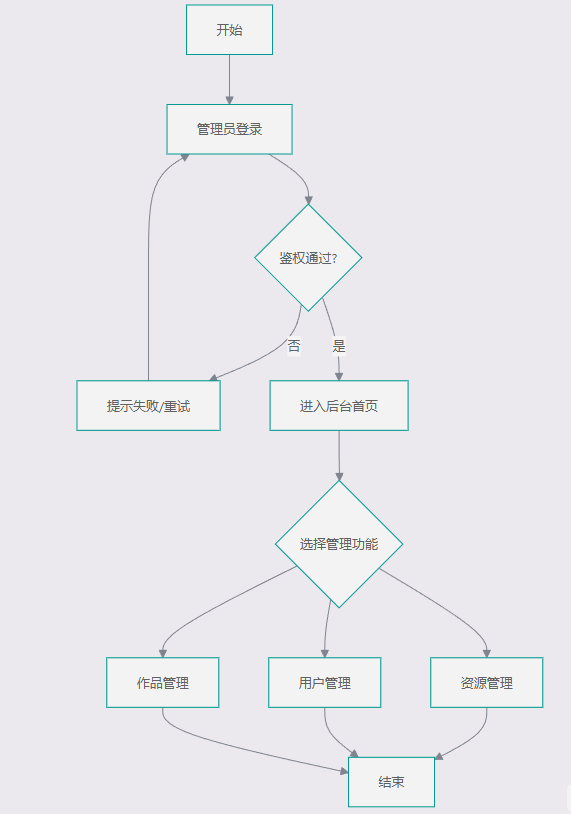
\includegraphics[width=\linewidth]{adminModuleFlow.png}
		\caption{后台管理流程图}
		\label{fig:adminModuleFlow}
	\end{minipage}
\end{figure}

模块流程描述：管理员登录后进入后台；在用户管理中可检索用户并执行角色分配，信息修改等操作；在作品审核中查看待审内容并做出通过或拒绝决定，必要时可对已发布内容执行下架；在资源管理中维护模型资源，保证前端定制能力与内容展示的基础数据完整。

\endgroup

\section{系统数据库设计}

\subsection{数据库实体联系分析}

根据第 3 章系统需求分析，得出以下结论：
\begin{itemize}
	\item 本系统数据库可划分为三个核心子域：用户域（\texttt{users}）、作品广场域（\texttt{design\_works} 及互动表）、任务域（\texttt{tryon\_tasks}），并由资源域（\texttt{model\_files}）提供文件支撑。
	\item \texttt{users} 为全局主体实体，承担身份认证与角色区分功能（普通用户/管理员），并作为作品发布、点赞、收藏、评论、试衣任务发起的统一行为主体。
	\item 为支持作者社交数据展示，\texttt{users} 表中引入 \texttt{followers\_count} 与 \texttt{following\_count} 两个冗余统计字段，用于快速展示用户的粉丝数与关注数，降低列表页聚合统计开销。
	\item \texttt{user\_follows} 用于记录用户之间的关注关系，以 \texttt{follower\_id} 与 \texttt{following\_id} 两个外键同时关联 \texttt{users}，通过唯一约束 \texttt{(follower\_id, following\_id)} 防止重复关注，并在用户注销时通过级联删除清理关注关系数据。
	\item \texttt{design\_works} 为业务核心实体，记录作品基础信息（标题、描述、状态、发布时间等），通过 \texttt{user\_id} 关联作品作者；通过 \texttt{cover\_file\_id} 关联封面资源。
	\item \texttt{model\_files} 用于统一管理文件资源（名称、URL、大小），在当前模型中主要被作品封面复用，形成“一个文件可被多个作品引用、一个作品最多一个封面文件”的关系。
	\item \texttt{work\_tags}、\texttt{work\_likes}、\texttt{work\_favorites}、\texttt{work\_comments} 构成作品互动子模型：标签表达作品的语义分类；点赞与收藏是用户与作品的多对多关系落地；评论表达用户对作品的一对多文本反馈。
	\item \texttt{tryon\_tasks} 表示用户针对作品触发的试衣生成任务，记录任务状态、进度、结果地址与异常信息，形成“用户—任务”“作品—任务”的双一对多关系。
	\item 一致性方面，互动表对作品设置了外键级联删除；同时点赞/收藏通过 \texttt{(work\_id, user\_id)} 唯一约束防止重复行为。\texttt{design\_works} 中的计数字段（点赞数、评论数、收藏数）属于冗余统计字段，用于提高查询性能。
\end{itemize}

\textbf{主要联系}
\begin{itemize}
	\item 用户 \texttt{users} 与作品 \texttt{design\_works}：1 对 N（一个用户可发布多个作品）。
	\item 用户 \texttt{users} 与关注关系 \texttt{user\_follows}：1 对 N（一个用户可发起多条关注关系）；用户 \texttt{users} 与关注关系 \texttt{user\_follows}：1 对 N（一个用户可被多条关注关系指向），从而在实体层面形成用户之间的 M 对 N 关注关系。
	\item 资源文件 \texttt{model\_files} 与作品 \texttt{design\_works}：1 对 N（一个文件可作为多个作品封面）。
	\item 作品 \texttt{design\_works} 与标签 \texttt{work\_tags}：1 对 N。
	\item 用户 \texttt{users} 与点赞 \texttt{work\_likes}：1 对 N；作品 \texttt{design\_works} 与点赞 \texttt{work\_likes}：1 对 N。
	\item 用户 \texttt{users} 与收藏 \texttt{work\_favorites}：1 对 N；作品 \texttt{design\_works} 与收藏 \texttt{work\_favorites}：1 对 N。
	\item 用户 \texttt{users} 与评论 \texttt{work\_comments}：1 对 N；作品 \texttt{design\_works} 与评论 \texttt{work\_comments}：1 对 N。
	\item 用户 \texttt{users} 与试衣任务 \texttt{tryon\_tasks}：1 对 N；作品 \texttt{design\_works} 与试衣任务 \texttt{tryon\_tasks}：1 对 N。
\end{itemize}

根据以上分析，系统的 ER 图如图~\ref{fig:er} 所示。

\begin{figure}[H]
	\centering
	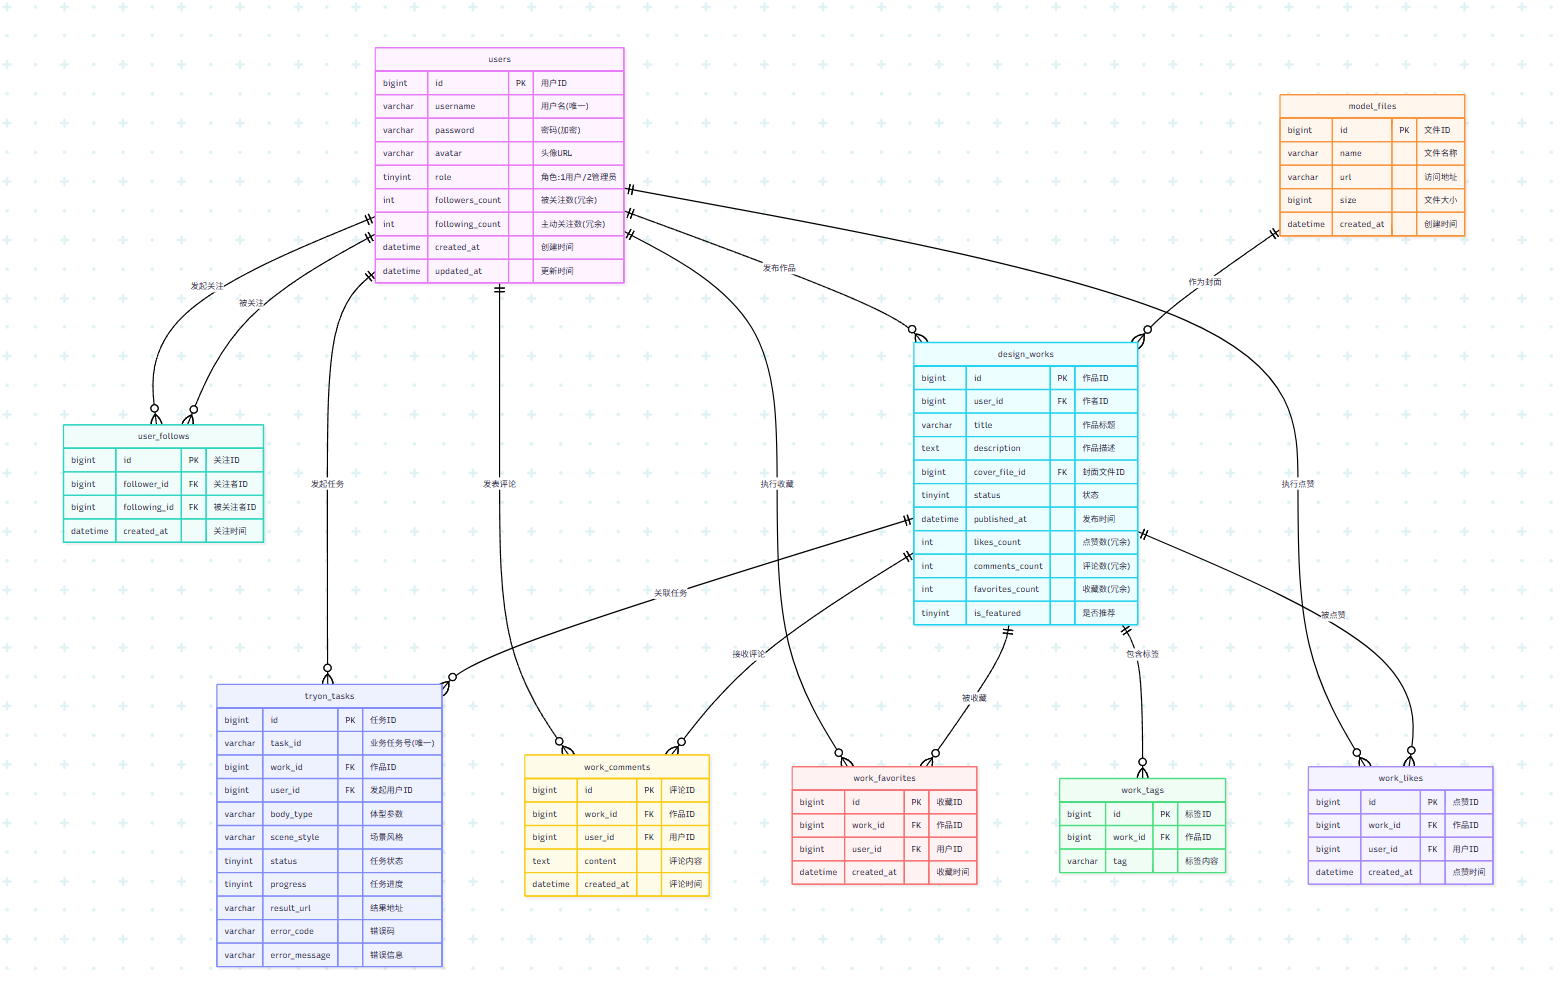
\includegraphics[width=0.88\textwidth]{ER.png}
	\caption{数据库 ER 图}
	\label{fig:er}
\end{figure}

\subsection{数据库核心数据表}

\noindent\textbf{（1）users（用户核心表）}

\noindent users（用户核心表）用于存储系统用户账号、密码、角色与基础资料，是全局用户主体表。系统通过 \texttt{user\_follows} 建立“用户\texorpdfstring{-}{-}用户”多对多关注关系，并引入 \texttt{followers\_count}/\texttt{following\_count} 作为冗余计数字段以降低列表页聚合统计开销；在关注/取关时同步更新被关注者 \texttt{followers\_count} 与关注者 \texttt{following\_count}。

users 表结构如表~\ref{tab:users} 所示。

{
\renewcommand{\arraystretch}{1.25}
\setlength{\tabcolsep}{0.2ex}
\begin{longtable}{@{}>{\raggedright\arraybackslash}p{0.16\textwidth} >{\raggedright\arraybackslash}p{0.18\textwidth} >{\raggedright\arraybackslash}p{0.30\textwidth} >{\raggedright\arraybackslash}p{0.32\textwidth}@{}}
\caption{users 表结构}\label{tab:users}\\
\toprule
字段名 & 类型 & 约束/索引 & 说明 \\
\midrule
\endfirsthead

\multicolumn{4}{c}{\zihao{5}续表\thetable\quad users 表结构}\\
\toprule
字段名 & 类型 & 约束/索引 & 说明 \\
\midrule
\endhead

\bottomrule
\endfoot

\bottomrule
\endlastfoot

\texttt{id} & \texttt{bigint(20) UNSIGNED} & \texttt{PK, AUTO\_INCREMENT} & 主键 ID \\
\texttt{username} & \texttt{varchar(50)} & \texttt{NOT NULL, UNIQUE(uk\_username)} & 登录用户名（唯一） \\
\texttt{password} & \texttt{varchar(255)} & \texttt{NOT NULL} & 加密后的密码 \\
\texttt{avatar} & \texttt{varchar(255)} & \texttt{DEFAULT NULL} & 头像 URL \\
\texttt{role} & \texttt{tinyint(2) UNSIGNED} & \texttt{NOT NULL, DEFAULT 1} & 角色：1\texorpdfstring{-}{-}普通用户，2\texorpdfstring{-}{-}管理员 \\
{\small\texttt{followers\_\allowbreak count}} & \texttt{int} & \texttt{NOT NULL, DEFAULT 0} & 被关注数（冗余统计） \\
{\small\texttt{following\_\allowbreak count}} & \texttt{int} & \texttt{NOT NULL, DEFAULT 0} & 主动关注数（冗余统计） \\
\texttt{created\_\allowbreak at} & \texttt{datetime} & \texttt{DEFAULT CURRENT\_TIMESTAMP} & 注册时间 \\
\texttt{updated\_\allowbreak at} & \texttt{datetime} & \texttt{DEFAULT CURRENT\_TIMESTAMP ON UPDATE CURRENT\_TIMESTAMP} & 最后更新时间 \\
\end{longtable}
}

\noindent\textbf{（2）user\_follows（用户关注关系表）}

\noindent user\_follows（用户关注关系表）用于记录用户之间的关注关系，以 \texttt{follower\_id} 与 \texttt{following\_id} 关联 \texttt{users}，支持关注/取关与关注列表/粉丝列表等功能，并通过唯一约束 \texttt{(follower\_id, following\_id)} 防止重复关注；用户注销时外键设置 \texttt{ON DELETE CASCADE} 以清理关联数据。

user\_follows 表结构如表~\ref{tab:user-follows} 所示。

{
\renewcommand{\arraystretch}{1.25}
\setlength{\tabcolsep}{0.2ex}
\begin{longtable}{@{}>{\raggedright\arraybackslash}p{0.14\textwidth} >{\raggedright\arraybackslash}p{0.18\textwidth} >{\raggedright\arraybackslash}p{0.30\textwidth} >{\raggedright\arraybackslash}p{0.32\textwidth}@{}}
\caption{user\_follows 表结构}\label{tab:user-follows}\\
\toprule
字段名 & 类型 & 约束/索引 & 说明 \\
\midrule
\endfirsthead

\multicolumn{4}{c}{\zihao{5}续表\thetable\quad user\_follows 表结构}\\
\toprule
字段名 & 类型 & 约束/索引 & 说明 \\
\midrule
\endhead

\bottomrule
\endfoot

\bottomrule
\endlastfoot

\texttt{id} & \texttt{bigint(20) UNSIGNED} & \texttt{PK, AUTO\_INCREMENT} & 主键 ID \\
\texttt{follower\_\allowbreak id} & \texttt{bigint(20) UNSIGNED} & \texttt{NOT NULL, KEY idx\_follower(follower\_id)} & 关注者 ID \\
\texttt{following\_\allowbreak id} & \texttt{bigint(20) UNSIGNED} & \texttt{NOT NULL, KEY idx\_following(following\_id)} & 被关注者 ID \\
\texttt{created\_\allowbreak at} & \texttt{datetime} & \texttt{DEFAULT CURRENT\_TIMESTAMP} & 关注时间 \\
\texttt{-} & \texttt{-} & \texttt{UNIQUE uk\_follower\_following(follower\_id, following\_id)} & 防止重复关注 \\
\texttt{-} & \texttt{-} & \texttt{FK follower\_id -> users(id) ON DELETE CASCADE} & 关注者外键 \\
\texttt{-} & \texttt{-} & \texttt{FK following\_id -> users(id) ON DELETE CASCADE} & 被关注者外键 \\
\end{longtable}
}

\noindent\textbf{（3）model\_files（模型/资源文件表）}

\noindent model\_files（模型/资源文件表）用于统一管理系统上传/生成的文件资源元数据，包括展示名称、访问 URL、文件大小以及创建/更新时间等信息，并作为各业务表引用外部资源的统一入口。当前模型中该表主要承载作品封面文件的引用关系，便于复用同一资源、减少冗余存储，同时通过名称索引支持后台按名称检索与管理。

model\_files 表结构如表~\ref{tab:model-files} 所示。

{
\renewcommand{\arraystretch}{1.25}
\setlength{\tabcolsep}{0.2ex}
\begin{longtable}{@{}>{\raggedright\arraybackslash}p{0.14\textwidth} >{\raggedright\arraybackslash}p{0.18\textwidth} >{\raggedright\arraybackslash}p{0.30\textwidth} >{\raggedright\arraybackslash}p{0.32\textwidth}@{}}
\caption{model\_files 表结构}\label{tab:model-files}\\
\toprule
字段名 & 类型 & 约束/索引 & 说明 \\
\midrule
\endfirsthead

\multicolumn{4}{c}{\zihao{5}续表\thetable\quad model\_files 表结构}\\
\toprule
字段名 & 类型 & 约束/索引 & 说明 \\
\midrule
\endhead

\bottomrule
\endfoot

\bottomrule
\endlastfoot

\texttt{id} & \texttt{bigint(20) UNSIGNED} & \texttt{PK, AUTO\_INCREMENT} & 主键 ID \\
\texttt{name} & \texttt{varchar(255)} & \texttt{NOT NULL, DEFAULT ''} & 展示名称 \\
\texttt{url} & \texttt{varchar(1024)} & \texttt{NOT NULL} & 访问 URL \\
\texttt{size} & \texttt{bigint(20) UNSIGNED} & \texttt{NOT NULL, DEFAULT 0} & 文件大小（byte） \\
\texttt{created\_\allowbreak at} & \texttt{datetime} & \texttt{DEFAULT CURRENT\_TIMESTAMP} & 创建时间 \\
\texttt{updated\_\allowbreak at} & \texttt{datetime} & \texttt{DEFAULT CURRENT\_TIMESTAMP ON UPDATE CURRENT\_TIMESTAMP} & 更新时间 \\
\texttt{-} & \texttt{-} & \texttt{KEY idx\_name(name)} & 名称索引 \\
\end{longtable}
}

\noindent\textbf{（4）design\_works（作品主表）}

\noindent design\_works（作品主表）用于存储作品主体信息，是创意广场的核心业务表，记录作品标题、描述、发布状态与发布时间等内容，并通过 \texttt{user\_id} 关联作品作者。该表可选关联封面文件 \texttt{cover\_file\_id}，并维护点赞数、评论数、收藏数等冗余统计字段与推荐标识，用于提升广场列表查询与排序展示的性能。

design\_works 表结构如表~\ref{tab:design-works} 所示。

{
\renewcommand{\arraystretch}{1.25}
\setlength{\tabcolsep}{0.2ex}
\begin{longtable}{@{}>{\raggedright\arraybackslash}p{0.16\textwidth} >{\raggedright\arraybackslash}p{0.20\textwidth} >{\raggedright\arraybackslash}p{0.30\textwidth} >{\raggedright\arraybackslash}p{0.28\textwidth}@{}}
\caption{design\_works 表结构}\label{tab:design-works}\\
\toprule
字段名 & 类型 & 约束/索引 & 说明 \\
\midrule
\endfirsthead

\multicolumn{4}{c}{\zihao{5}续表\thetable\quad design\_works 表结构}\\
\toprule
字段名 & 类型 & 约束/索引 & 说明 \\
\midrule
\endhead

\bottomrule
\endfoot

\bottomrule
\endlastfoot

\texttt{id} & \texttt{bigint(20) UNSIGNED} & \texttt{PK, AUTO\_INCREMENT} & 作品 ID \\
\texttt{user\_\allowbreak id} & \texttt{bigint(20) UNSIGNED} & \texttt{NOT NULL, KEY idx\_user(user\_id)} & 作者用户 ID \\
\texttt{title} & \texttt{varchar(255)} & \texttt{NOT NULL, DEFAULT ''} & 作品标题 \\
\texttt{description} & \texttt{text} & \texttt{-} & 作品描述 \\
\texttt{cover\_\allowbreak file\_\allowbreak id} & \texttt{bigint(20) UNSIGNED} & \texttt{DEFAULT NULL} & 封面文件 ID \\
\texttt{status} & \texttt{tinyint(3) UNSIGNED} & \texttt{NOT NULL, DEFAULT 1, KEY idx\_status(status)} & 作品状态 \\
\texttt{published\_\allowbreak at} & \texttt{datetime} & \texttt{DEFAULT NULL} & 发布时间 \\
\texttt{created\_\allowbreak at} & \texttt{datetime} & \texttt{DEFAULT CURRENT\_TIMESTAMP} & 创建时间 \\
\texttt{updated\_\allowbreak at} & \texttt{datetime} & \texttt{DEFAULT CURRENT\_TIMESTAMP ON UPDATE CURRENT\_TIMESTAMP} & 更新时间 \\
\texttt{likes\_\allowbreak count} & \texttt{int} & \texttt{NOT NULL, DEFAULT 0} & 点赞数（冗余统计） \\
\texttt{comments\_\allowbreak count} & \texttt{int} & \texttt{NOT NULL, DEFAULT 0} & 评论数（冗余统计） \\
\texttt{favorites\_\allowbreak count} & \texttt{int} & \texttt{NOT NULL, DEFAULT 0} & 收藏数（冗余统计） \\
\texttt{is\_\allowbreak featured} & \texttt{tinyint(1)} & \texttt{NOT NULL, DEFAULT 0} & 是否推荐 \\
\end{longtable}
}

\noindent\textbf{（5）work\_tags（作品标签表）}

\noindent work\_tags（作品标签表）用于维护作品与标签的关联，将作品与若干语义标签进行绑定，以支撑分类浏览、条件筛选与个性化推荐等功能。表中通过 \texttt{work\_id} 快速定位作品标签集合，并为 \texttt{tag} 建立索引以提高按标签聚合与检索的效率。

work\_tags 表结构如表~\ref{tab:work-tags} 所示。

{
\renewcommand{\arraystretch}{1.25}
\setlength{\tabcolsep}{0.2ex}
\begin{longtable}{@{}>{\raggedright\arraybackslash}p{0.14\textwidth} >{\raggedright\arraybackslash}p{0.20\textwidth} >{\raggedright\arraybackslash}p{0.34\textwidth} >{\raggedright\arraybackslash}p{0.28\textwidth}@{}}
\caption{work\_tags 表结构}\label{tab:work-tags}\\
\toprule
字段名 & 类型 & 约束/索引 & 说明 \\
\midrule
\endfirsthead

\multicolumn{4}{c}{\zihao{5}续表\thetable\quad work\_tags 表结构}\\
\toprule
字段名 & 类型 & 约束/索引 & 说明 \\
\midrule
\endhead

\bottomrule
\endfoot

\bottomrule
\endlastfoot

\texttt{id} & \texttt{bigint(20) UNSIGNED} & \texttt{PK, AUTO\_INCREMENT} & 主键 ID \\
\texttt{work\_\allowbreak id} & \texttt{bigint(20) UNSIGNED} & \texttt{NOT NULL, FK->design\_works(id), INDEX idx\_work\_id(work\_id)} & 作品 ID \\
\texttt{tag} & \texttt{varchar(32)} & \texttt{NOT NULL, INDEX idx\_tag(tag)} & 标签内容 \\
\end{longtable}
}

\noindent\textbf{（6）work\_likes（作品点赞表）}

\noindent work\_likes（作品点赞表）用于记录用户对作品的点赞行为，形成“用户\texorpdfstring{-}{-}作品”的多对多关系落地数据，用于支撑点赞/取消点赞以及点赞列表查询等功能。该表通过唯一约束 \texttt{(work\_id, user\_id)} 防止重复点赞，并以时间字段记录行为发生时间，便于行为追溯与排序展示。

work\_likes 表结构如表~\ref{tab:work-likes} 所示。

{
\renewcommand{\arraystretch}{1.25}
\setlength{\tabcolsep}{0.2ex}
\begin{longtable}{@{}>{\raggedright\arraybackslash}p{0.14\textwidth} >{\raggedright\arraybackslash}p{0.20\textwidth} >{\raggedright\arraybackslash}p{0.34\textwidth} >{\raggedright\arraybackslash}p{0.28\textwidth}@{}}
\caption{work\_likes 表结构}\label{tab:work-likes}\\
\toprule
字段名 & 类型 & 约束/索引 & 说明 \\
\midrule
\endfirsthead

\multicolumn{4}{c}{\zihao{5}续表\thetable\quad work\_likes 表结构}\\
\toprule
字段名 & 类型 & 约束/索引 & 说明 \\
\midrule
\endhead

\bottomrule
\endfoot

\bottomrule
\endlastfoot

\texttt{id} & \texttt{bigint(20) UNSIGNED} & \texttt{PK, AUTO\_INCREMENT} & 主键 ID \\
\texttt{work\_\allowbreak id} & \texttt{bigint(20) UNSIGNED} & \texttt{NOT NULL, FK->design\_works(id)} & 作品 ID \\
\texttt{user\_\allowbreak id} & \texttt{bigint(20) UNSIGNED} & \texttt{NOT NULL} & 点赞用户 ID \\
\texttt{created\_\allowbreak at} & \texttt{datetime} & \texttt{DEFAULT CURRENT\_TIMESTAMP} & 点赞时间 \\
\texttt{-} & \texttt{-} & \texttt{UNIQUE uk\_work\_user(work\_id, user\_id)} & 防止重复点赞 \\
\end{longtable}
}

\noindent\textbf{（7）work\_favorites（作品收藏表）}

\noindent work\_favorites（作品收藏表）用于记录用户对作品的收藏行为，支撑用户收藏夹、收藏/取消收藏与收藏状态判断等功能，并在数据层面表达“用户\texorpdfstring{-}{-}作品”多对多关系。该表同样通过唯一约束 \texttt{(work\_id, user\_id)} 防止重复收藏，并使用时间字段记录收藏发生时间，便于收藏列表按时间排序。

work\_favorites 表结构如表~\ref{tab:work-favorites} 所示。

{
\renewcommand{\arraystretch}{1.25}
\setlength{\tabcolsep}{0.2ex}
\begin{longtable}{@{}>{\raggedright\arraybackslash}p{0.14\textwidth} >{\raggedright\arraybackslash}p{0.20\textwidth} >{\raggedright\arraybackslash}p{0.34\textwidth} >{\raggedright\arraybackslash}p{0.28\textwidth}@{}}
\caption{work\_favorites 表结构}\label{tab:work-favorites}\\
\toprule
字段名 & 类型 & 约束/索引 & 说明 \\
\midrule
\endfirsthead

\multicolumn{4}{c}{\zihao{5}续表\thetable\quad work\_favorites 表结构}\\
\toprule
字段名 & 类型 & 约束/索引 & 说明 \\
\midrule
\endhead

\bottomrule
\endfoot

\bottomrule
\endlastfoot

\texttt{id} & \texttt{bigint(20) UNSIGNED} & \texttt{PK, AUTO\_INCREMENT} & 主键 ID \\
\texttt{work\_\allowbreak id} & \texttt{bigint(20) UNSIGNED} & \texttt{NOT NULL, FK->design\_works(id)} & 作品 ID \\
\texttt{user\_\allowbreak id} & \texttt{bigint(20) UNSIGNED} & \texttt{NOT NULL} & 收藏用户 ID \\
\texttt{created\_\allowbreak at} & \texttt{datetime} & \texttt{DEFAULT CURRENT\_TIMESTAMP} & 收藏时间 \\
\texttt{-} & \texttt{-} & \texttt{UNIQUE uk\_work\_user(work\_id, user\_id)} & 防止重复收藏 \\
\end{longtable}
}

\noindent\textbf{（8）work\_comments（作品评论表）}

\noindent work\_comments（作品评论表）用于记录用户对作品的文本评论内容，支撑作品详情页评论展示、评论发布与评论列表分页查询等功能。该表通过 \texttt{work\_id} 关联评论所属作品、通过 \texttt{user\_id} 标识评论作者，并对 \texttt{work\_id} 建立索引以优化按作品维度的评论检索。

work\_comments 表结构如表~\ref{tab:work-comments} 所示。

{
\renewcommand{\arraystretch}{1.25}
\setlength{\tabcolsep}{0.2ex}
\begin{longtable}{@{}>{\raggedright\arraybackslash}p{0.14\textwidth} >{\raggedright\arraybackslash}p{0.20\textwidth} >{\raggedright\arraybackslash}p{0.34\textwidth} >{\raggedright\arraybackslash}p{0.28\textwidth}@{}}
\caption{work\_comments 表结构}\label{tab:work-comments}\\
\toprule
字段名 & 类型 & 约束/索引 & 说明 \\
\midrule
\endfirsthead

\multicolumn{4}{c}{\zihao{5}续表\thetable\quad work\_comments 表结构}\\
\toprule
字段名 & 类型 & 约束/索引 & 说明 \\
\midrule
\endhead

\bottomrule
\endfoot

\bottomrule
\endlastfoot

\texttt{id} & \texttt{bigint(20) UNSIGNED} & \texttt{PK, AUTO\_INCREMENT} & 主键 ID \\
\texttt{work\_\allowbreak id} & \texttt{bigint(20) UNSIGNED} & \texttt{NOT NULL, FK->design\_works(id), INDEX idx\_work\_id(work\_id)} & 作品 ID \\
\texttt{user\_\allowbreak id} & \texttt{bigint(20) UNSIGNED} & \texttt{NOT NULL} & 评论用户 ID \\
\texttt{content} & \texttt{text} & \texttt{NOT NULL} & 评论内容 \\
\texttt{created\_\allowbreak at} & \texttt{datetime} & \texttt{DEFAULT CURRENT\_TIMESTAMP} & 评论时间 \\
\end{longtable}
}

\noindent\textbf{（9）tryon\_tasks（试衣任务表）}

\noindent tryon\_tasks（试衣任务表）用于记录用户针对作品发起的试衣生成任务及执行结果，支撑异步任务创建、进度查询与结果展示等流程，并通过唯一的业务任务号 \texttt{task\_id} 进行幂等与外部调用关联。该表记录输入参考数据、任务状态与进度、结果地址以及异常信息，同时保存开始/完成时间与创建/更新时间，用于任务调度、失败重试与问题定位。

tryon\_tasks 表结构如表~\ref{tab:tryon-tasks} 所示。

{
\renewcommand{\arraystretch}{1.25}
\setlength{\tabcolsep}{0.2ex}
\begin{longtable}{@{}>{\raggedright\arraybackslash}p{0.16\textwidth} >{\raggedright\arraybackslash}p{0.20\textwidth} >{\raggedright\arraybackslash}p{0.34\textwidth} >{\raggedright\arraybackslash}p{0.26\textwidth}@{}}
\caption{tryon\_tasks 表结构}\label{tab:tryon-tasks}\\
\toprule
字段名 & 类型 & 约束/索引 & 说明 \\
\midrule
\endfirsthead

\multicolumn{4}{c}{\zihao{5}续表\thetable\quad tryon\_tasks 表结构}\\
\toprule
字段名 & 类型 & 约束/索引 & 说明 \\
\midrule
\endhead

\bottomrule
\endfoot

\bottomrule
\endlastfoot

\texttt{id} & \texttt{bigint(20) UNSIGNED} & \texttt{PK, AUTO\_INCREMENT} & 主键 ID \\
\texttt{task\_\allowbreak id} & \texttt{varchar(64)} & \texttt{NOT NULL, UNIQUE uk\_task\_id(task\_id)} & 业务任务号 \\
\texttt{work\_\allowbreak id} & \texttt{bigint(20) UNSIGNED} & \texttt{NOT NULL, KEY idx\_work\_id(work\_id)} & 关联作品 ID \\
\texttt{user\_\allowbreak id} & \texttt{bigint(20) UNSIGNED} & \texttt{NOT NULL, KEY idx\_user\_id(user\_id)} & 发起用户 ID \\
\texttt{gender} & \texttt{varchar(64)} & \texttt{NOT NULL, DEFAULT ''} & 性别 \\
\texttt{body\_\allowbreak type} & \texttt{varchar(64)} & \texttt{NOT NULL, DEFAULT ''} & 体型参数 \\
\texttt{scene\_\allowbreak style} & \texttt{varchar(64)} & \texttt{NOT NULL, DEFAULT ''} & 场景风格 \\
\texttt{input\_\allowbreak refs} & \texttt{json} & \texttt{NOT NULL} & 输入参考数据 \\
\texttt{status} & \texttt{tinyint(3) UNSIGNED} & \texttt{NOT NULL, DEFAULT 1, KEY idx\_status(status)} & 任务状态 \\
\texttt{progress} & \texttt{tinyint(3) UNSIGNED} & \texttt{NOT NULL, DEFAULT 0} & 任务进度 \\
\texttt{result\_\allowbreak url} & \texttt{varchar(1024)} & \texttt{NOT NULL, DEFAULT ''} & 结果地址 \\
\texttt{error\_\allowbreak code} & \texttt{varchar(64)} & \texttt{NOT NULL, DEFAULT ''} & 错误码 \\
\texttt{error\_\allowbreak message} & \texttt{varchar(1024)} & \texttt{NOT NULL, DEFAULT ''} & 错误信息 \\
\texttt{started\_\allowbreak at} & \texttt{datetime} & \texttt{DEFAULT NULL} & 开始时间 \\
\texttt{finished\_\allowbreak at} & \texttt{datetime} & \texttt{DEFAULT NULL} & 完成时间 \\
\texttt{created\_\allowbreak at} & \texttt{datetime} & \texttt{DEFAULT CURRENT\_TIMESTAMP, KEY idx\_created\_at(created\_at)} & 创建时间 \\
\texttt{updated\_\allowbreak at} & \texttt{datetime} & \texttt{DEFAULT CURRENT\_TIMESTAMP ON UPDATE CURRENT\_TIMESTAMP} & 更新时间 \\
\end{longtable}
}

\chapter{系统实现}

\section{系统开发环境}

本项目采用前后端分离架构，后端基于 \textbf{Go + Gin}，前端采用 \textbf{Vue 3 + Nuxt 3}。开发环境配置如下：

\begin{enumerate}[label=(\arabic*)]
	\item \textbf{硬件环境} 选择 Intel Core i7 及以上级别 CPU、16GB 及以上内存、512GB 及以上 SSD 的开发主机，以保障本地数据库、缓存服务和前端构建任务并行运行的稳定性。
	\item \textbf{操作系统} 选择 \textbf{Windows 10/11} 作为主要开发平台（兼容 Linux/macOS 开发环境），满足 Go、Node.js、MySQL、Redis 等组件的安装与运行要求。
	\item \textbf{前端技术栈} 选择 \textbf{Vue 3} 作为前端核心框架，\textbf{Nuxt 3} 作为应用框架（支持 SSR/CSR 混合渲染），并结合 TypeScript 进行工程化开发。
	\item \textbf{后端技术栈} 选择 \textbf{Go 1.25.x} 作为后端开发语言，\textbf{Gin} 作为 Web 框架，提供 RESTful API 服务\cite{fielding2000rest}。
	\item \textbf{数据存储与缓存} 选择 \textbf{MySQL 8.x} 作为关系型数据库，\textbf{Redis 7.x} 作为缓存与状态加速组件，提升高频查询与会话相关操作性能。
	\item \textbf{对象存储服务} 选择 \textbf{阿里云 OSS} 作为文件存储服务，用于模型文件、作品资源及结果文件的统一管理与访问。
	\item \textbf{项目依赖与构建工具} 后端使用 \textbf{Go Modules} 进行依赖管理；前端使用 \textbf{Node.js 20 LTS + pnpm/npm} 进行依赖安装与构建管理。
	\item \textbf{开发工具与辅助软件} 后端开发可使用 \textbf{GoLand / VS Code}，前端开发使用 \textbf{VS Code（Vue/Nuxt 插件）}；数据库管理使用 \textbf{Navicat / DataGrip}；接口联调使用 \textbf{Apifox / Postman}；版本管理使用 \textbf{Git}。
\end{enumerate}

\section{系统功能模块实现}

本系统采用前后端分离架构实现：前台用户端基于 Vue3 + Nuxt3，负责页面渲染、交互逻辑与接口调用；后端基于 Go + Gin，负责业务处理、权限控制、数据持久化与异步任务调度。各功能模块均通过 RESTful API 对外提供服务，前端通过 JWT 完成登录态管理与受限资源访问。

\subsection{用户管理模块实现}

用户管理模块涉及前台认证与用户信息维护，后端核心对象为 \texttt{AuthController}、\texttt{User} 数据模型以及 JWT/密码工具组件。前端 Nuxt3 通过登录页、注册页和个人中心页调用用户接口，实现身份认证与资料维护。用户管理模块接口如表~\ref{tab:api-user} 所示。此部分的核心代码参看附录A 

\begin{table}[H]
	\centering
	\caption{用户管理模块接口}
	\label{tab:api-user}
	\renewcommand{\arraystretch}{1.25}
	\setlength{\tabcolsep}{0.2ex}
	\begin{tabularx}{\textwidth}{@{}>{\raggedright\arraybackslash}p{0.26\textwidth} >{\raggedright\arraybackslash}X >{\centering\arraybackslash}p{0.14\textwidth}@{}}
		\toprule
		功能说明 & 接口 API & Http 方法 \\
		\midrule
		用户注册 & \texttt{/api/front/register} & POST \\
		用户登录 & \texttt{/api/front/login} & POST \\
		查询个人信息 & \texttt{/api/front/me} & GET \\
		修改个人信息/密码 & \texttt{/api/front/me} & POST \\
		上传用户头像 & \texttt{/api/front/me/avatar} & POST \\
		\bottomrule
	\end{tabularx}
\end{table}

根据以上接口，用户模块登录与认证实现过程如下：
\begin{enumerate}[label=(\arabic*)]
	\item 前端提交用户名与密码到登录接口；
	\item 后端校验参数完整性，按用户名查询用户记录；
	\item 使用密码哈希比对算法验证口令正确性；
	\item 校验通过后生成 JWT Token，并返回用户基础信息；
	\item 前端保存 Token（如 Pinia + LocalStorage/Cookie），后续请求统一携带 \texttt{Authorization: Bearer \textless token\textgreater}；
	\item 受保护接口通过认证中间件解析 Token，将 \texttt{userID/role} 写入上下文；
	\item 前端根据返回结果提示用户“登录成功/失败”，并完成页面跳转与登录态刷新，界面如图~\ref{fig:impl-login}所示。
\end{enumerate}

\begin{figure}[H]
	\centering
	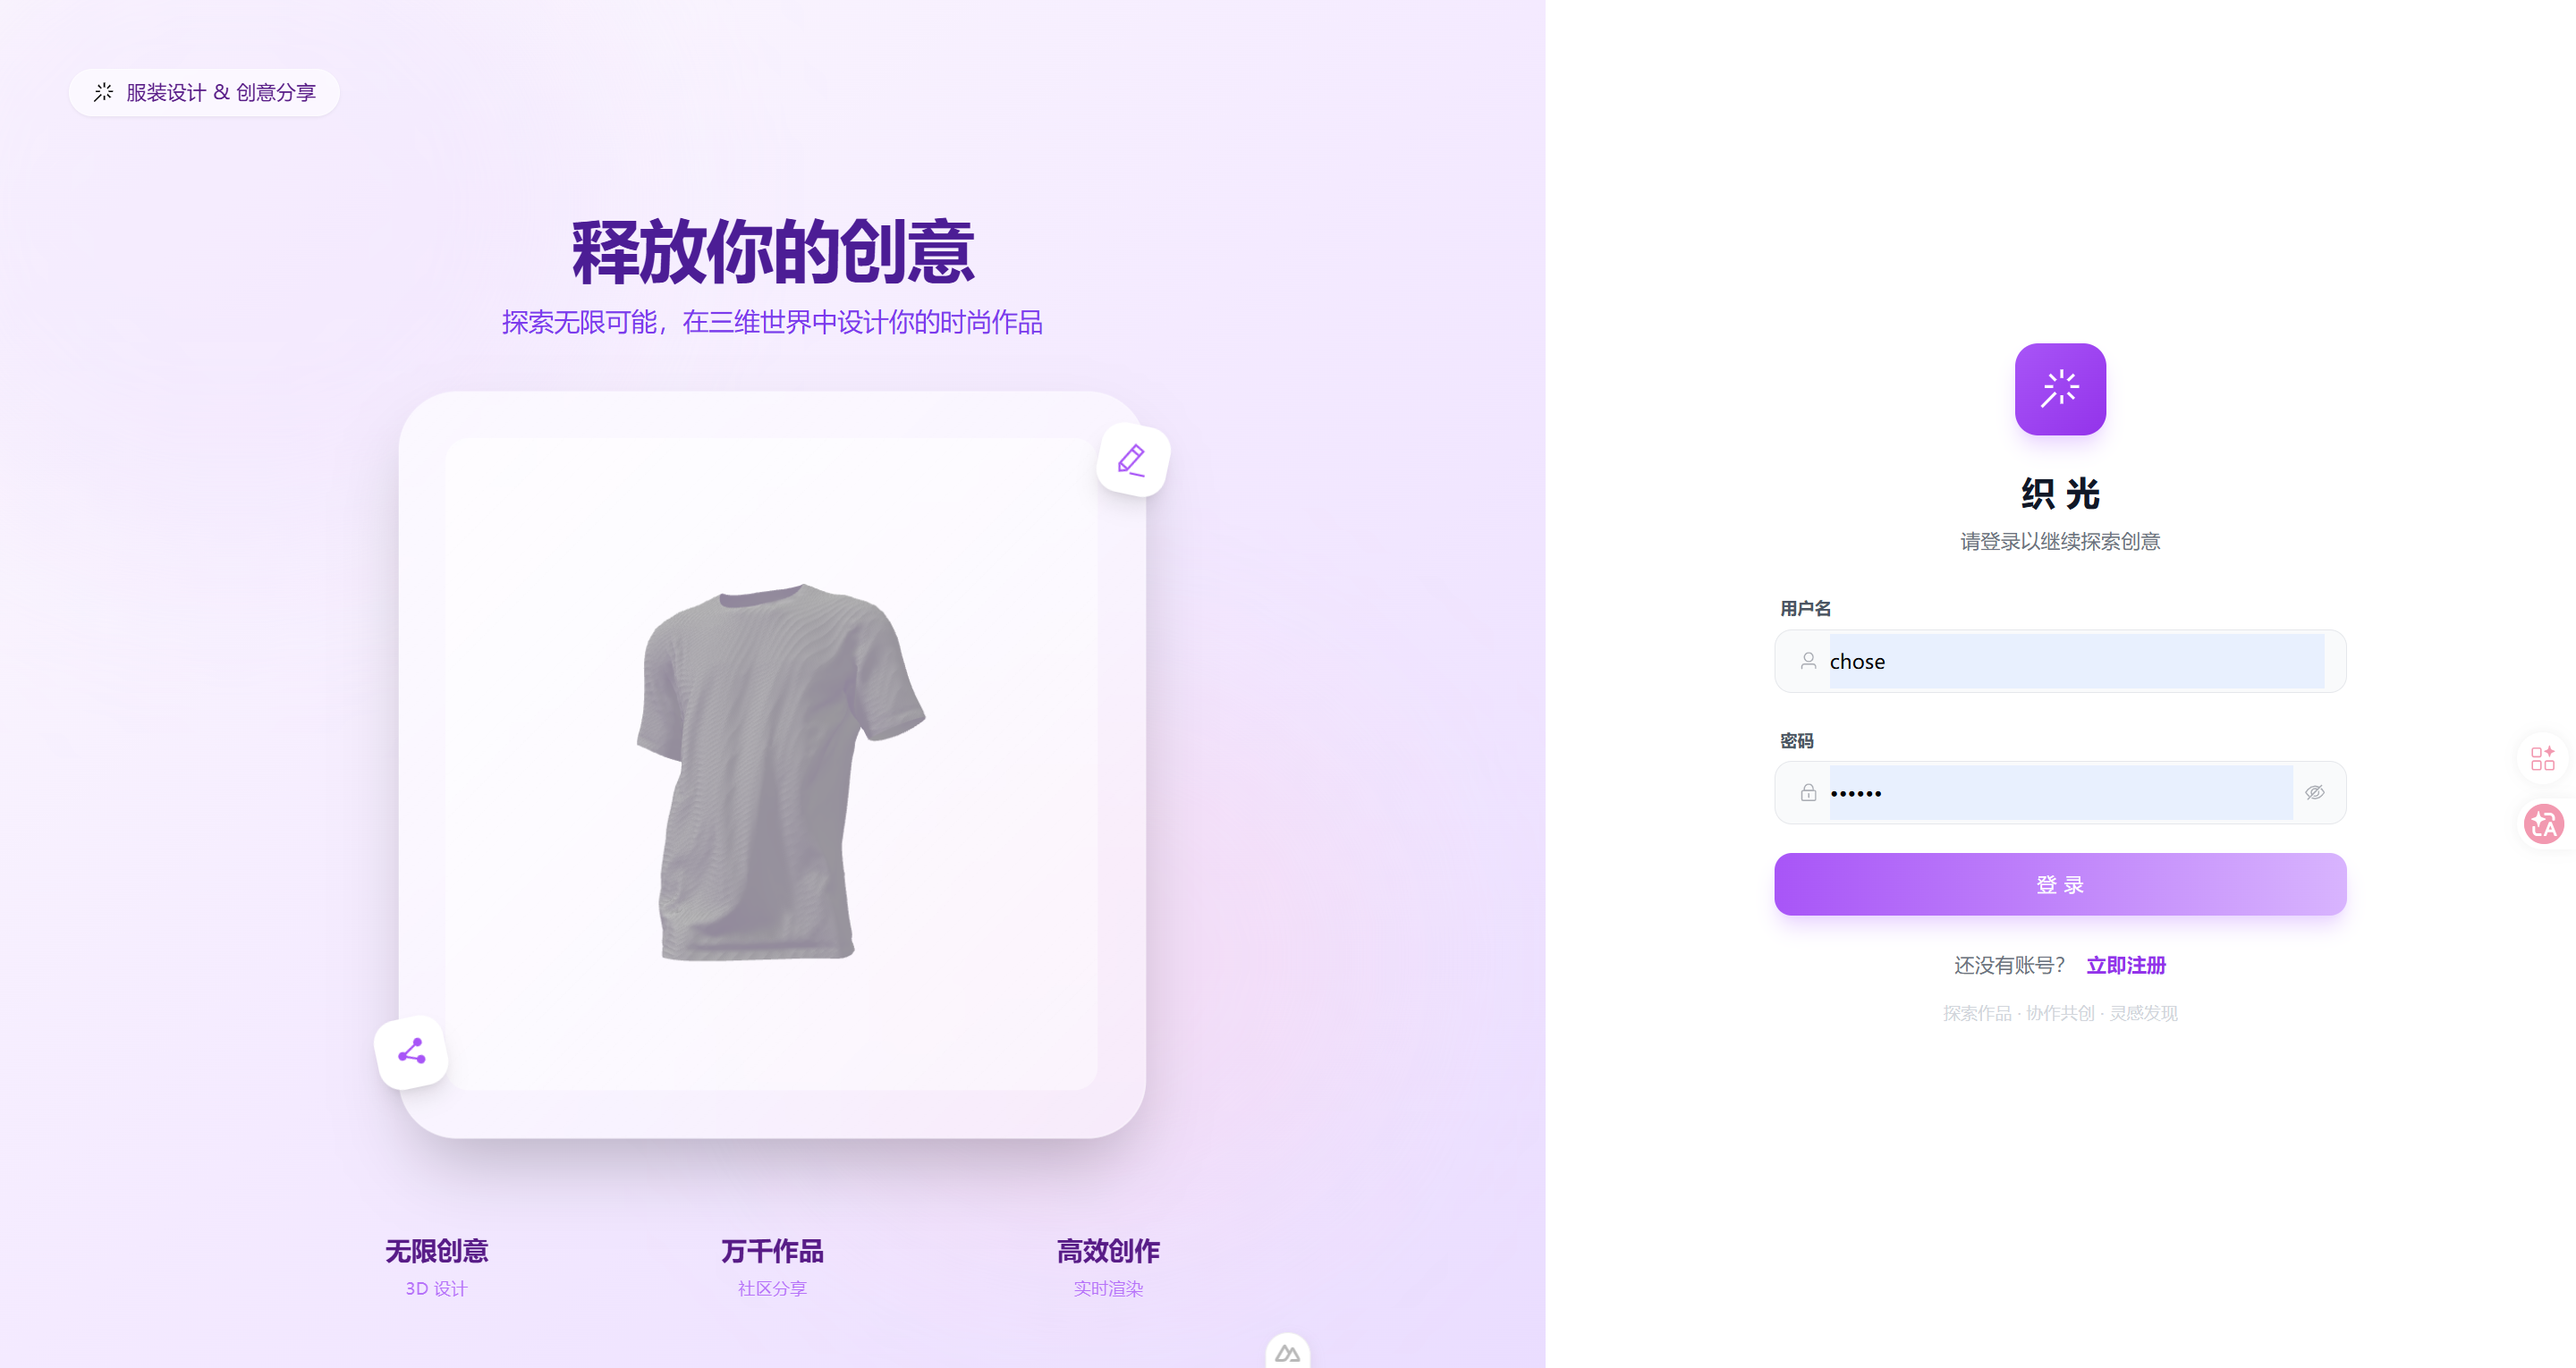
\includegraphics[width=0.85\textwidth]{login.png}
	\caption{用户登录}
	\label{fig:impl-login}
\end{figure}

\subsection{3D 服装定制模块实现}

3D 服装定制模块用于实现服装参数化设计与模板选择。前端提供参数面板和设计表单，同时通过 Three.js 渲染模型；后端维护作品草稿、定制参数及模型资源引用，实现“创建—编辑—保存”的设计闭环。3D 服装定制模块接口如表~\ref{tab:api-3d} 所示。此部分的核心代码参看附录B

\begin{table}[H]
	\centering
	\caption{3D 服装定制模块接口}
	\label{tab:api-3d}
	\renewcommand{\arraystretch}{1.25}
	\setlength{\tabcolsep}{0.2ex}
	\begin{tabularx}{\textwidth}{@{}>{\raggedright\arraybackslash}p{0.26\textwidth} >{\raggedright\arraybackslash}X >{\centering\arraybackslash}p{0.14\textwidth}@{}}
		\toprule
		功能说明 & 接口 API & Http 方法 \\
		\midrule
		模板资源列表 & \texttt{/api/front/templates} & GET \\
		新建定制作品 & \texttt{/api/front/works} & POST \\
		更新定制作品 & \texttt{/api/front/works/:id} & POST \\
		设置作品标签 & \texttt{/api/front/works/:id/tags} & POST \\
		\bottomrule
	\end{tabularx}
\end{table}

该模块实现过程如下：
\begin{enumerate}[label=(\arabic*)]
	\item 前端先请求模板列表，加载可选模型资源；
	\item 用户填写标题、描述、封面并配置 \texttt{params\_json} 参数；
	\item 后端创建作品主记录，并写入初始设计参数；
	\item 用户二次编辑时，后端按作品状态判断是否允许修改；
	\item 驳回后重编辑会自动回到草稿态，便于再次提交；
	\item 标签信息独立维护，支持后续广场检索与分类展示；
	\item 前端根据保存结果实时刷新设计视图与作品状态，界面如图~\ref{fig:impl-3d}所示。
\end{enumerate}

\begin{figure}[H]
	\centering
	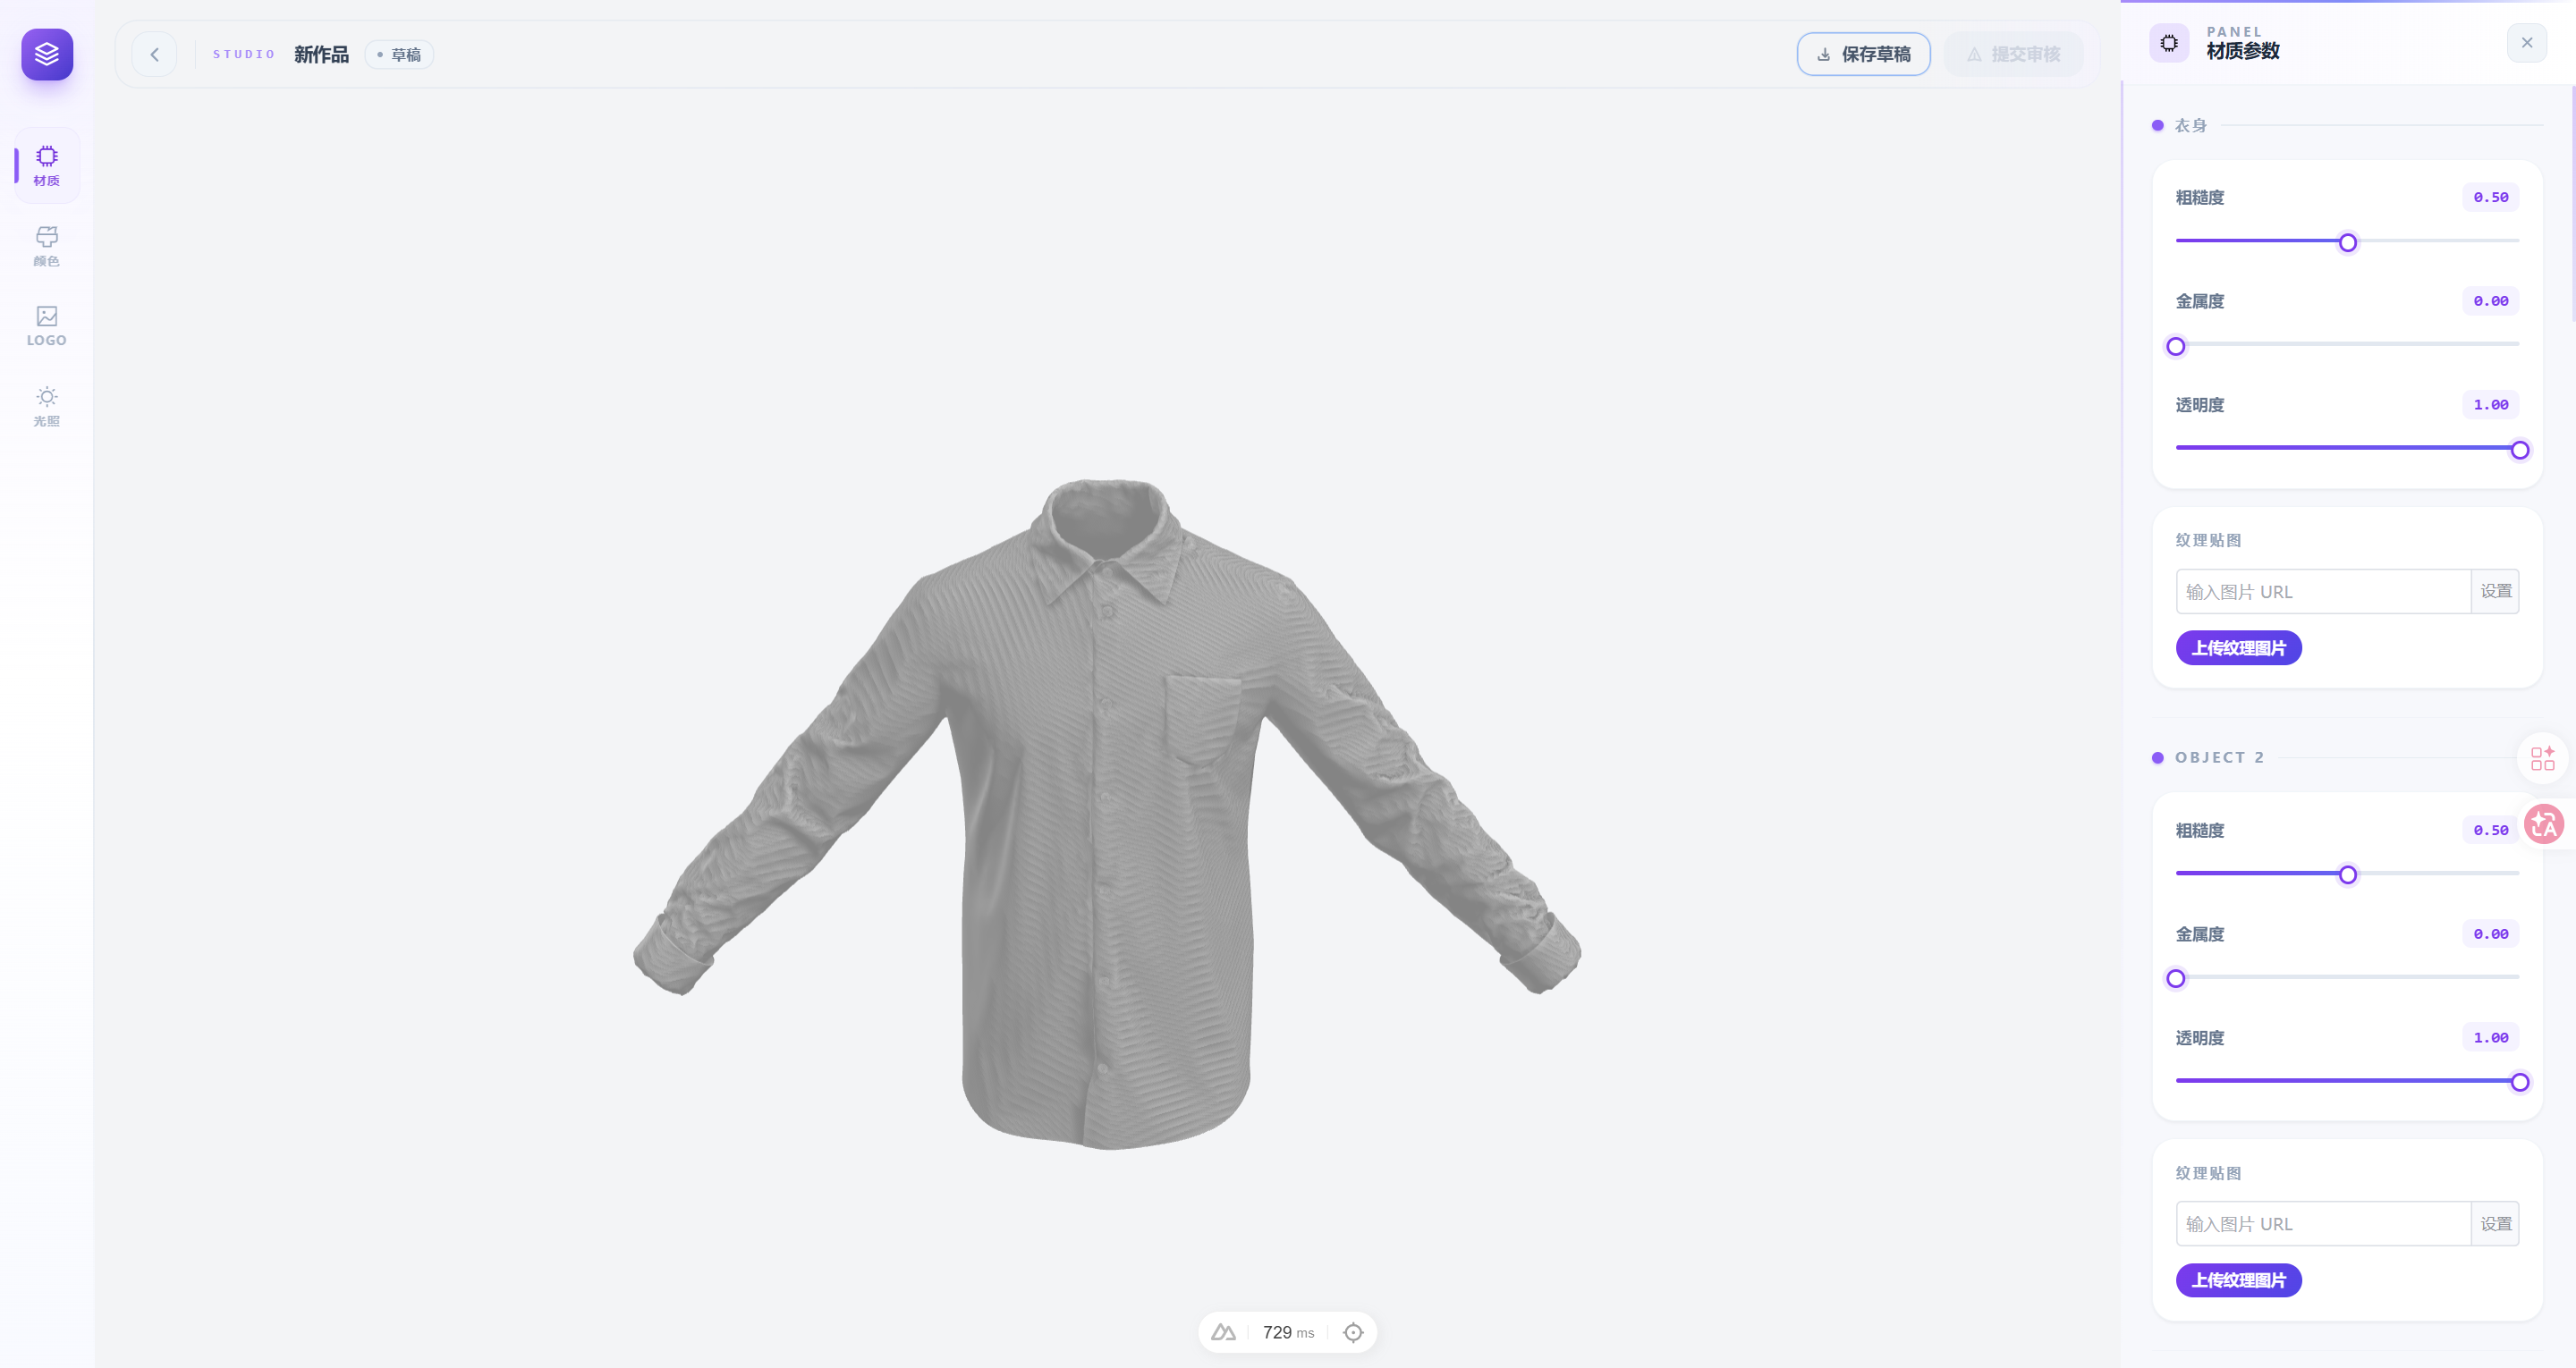
\includegraphics[width=0.85\textwidth]{3d.png}
	\caption{3D 服装定制}
	\label{fig:impl-3d}
\end{figure}

\subsection{AI 虚拟试穿模块实现}

AI 虚拟试穿模块采用异步任务架构，服务端由”任务创建接口 + Worker 消费进程”构成。前端 Nuxt3 负责提交试穿参数并轮询任务状态，完成结果展示。本模块参考了 DrapeNet\cite{drapenet_garment_generation}的服装生成与自监督拟合思路，结合扩散模型进行真人效果合成，生成图像质量采用结构相似性（SSIM）\cite{wang2004ssim}等指标衡量。AI 虚拟试穿模块接口如表~\ref{tab:api-tryon} 所示。此部分的核心代码参看附录C

\begin{table}[H]
	\centering
	\caption{AI 虚拟试穿模块接口}
	\label{tab:api-tryon}
	\renewcommand{\arraystretch}{1.25}
	\setlength{\tabcolsep}{0.2ex}
	\begin{tabularx}{\textwidth}{@{}>{\raggedright\arraybackslash}p{0.26\textwidth} >{\raggedright\arraybackslash}X >{\centering\arraybackslash}p{0.14\textwidth}@{}}
		\toprule
		功能说明 & 接口 API & Http 方法 \\
		\midrule
		创建试穿任务 & \texttt{/api/front/works/:id/tryon/tasks} & POST \\
		查询任务状态 & \texttt{/api/front/works/:id/tryon/tasks/:task\_id} & GET \\
		\bottomrule
	\end{tabularx}
\end{table}

该模块实现过程如下：
\begin{enumerate}[label=(\arabic*)]
	\item 前端提交体型参数、场景风格与参考输入数据；
	\item 后端校验用户权限、作品归属与任务并发限制；
	\item 创建试穿任务记录，状态置为“排队中”；
	\item 任务写入 Redis 队列，由 Worker 异步消费；
	\item Worker 调用 AI 推理服务，更新执行进度与运行状态；
	\item 执行成功后写入结果地址，失败则记录错误码并重试/终止；
	\item 前端轮询任务接口，根据状态与进度更新 UI 并展示试穿结果图，界面如图~\ref{fig:impl-tryon-queue}、图~\ref{fig:impl-tryon-result}所示。
\end{enumerate}

\begin{figure}[H]
	\centering
	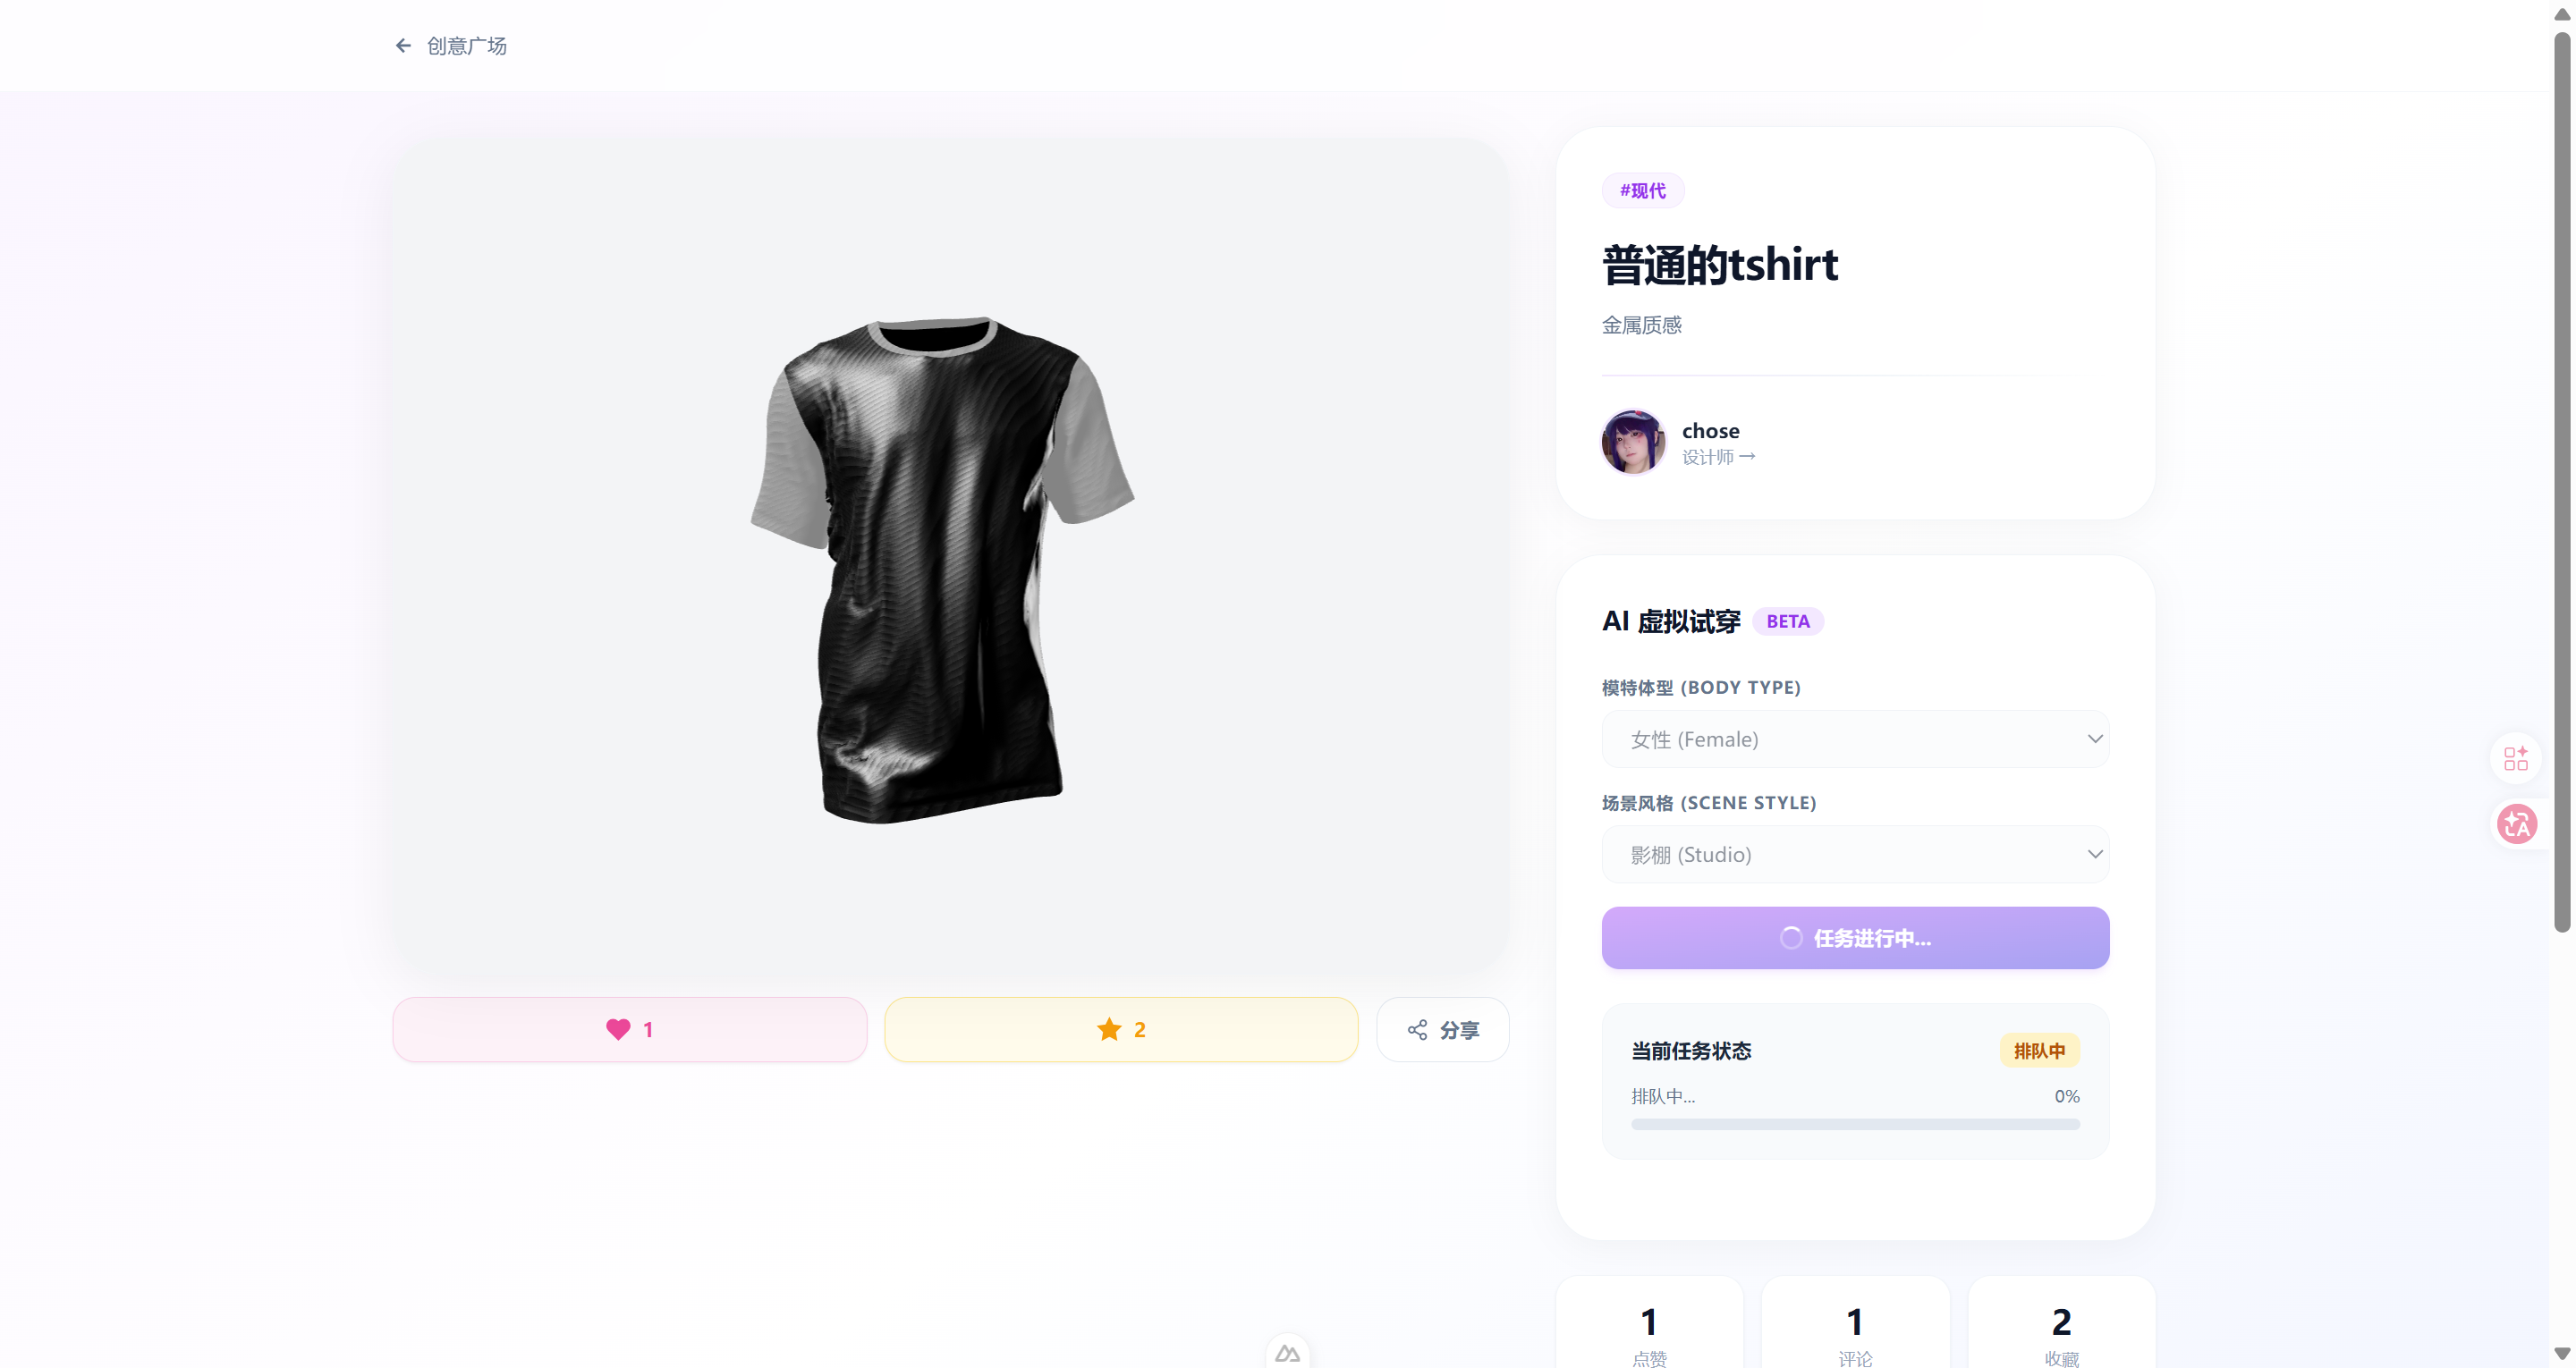
\includegraphics[width=0.85\textwidth]{AI1.png}
	\caption{AI 虚拟试穿生成排队}
	\label{fig:impl-tryon-queue}
\end{figure}

\begin{figure}[H]
	\centering
	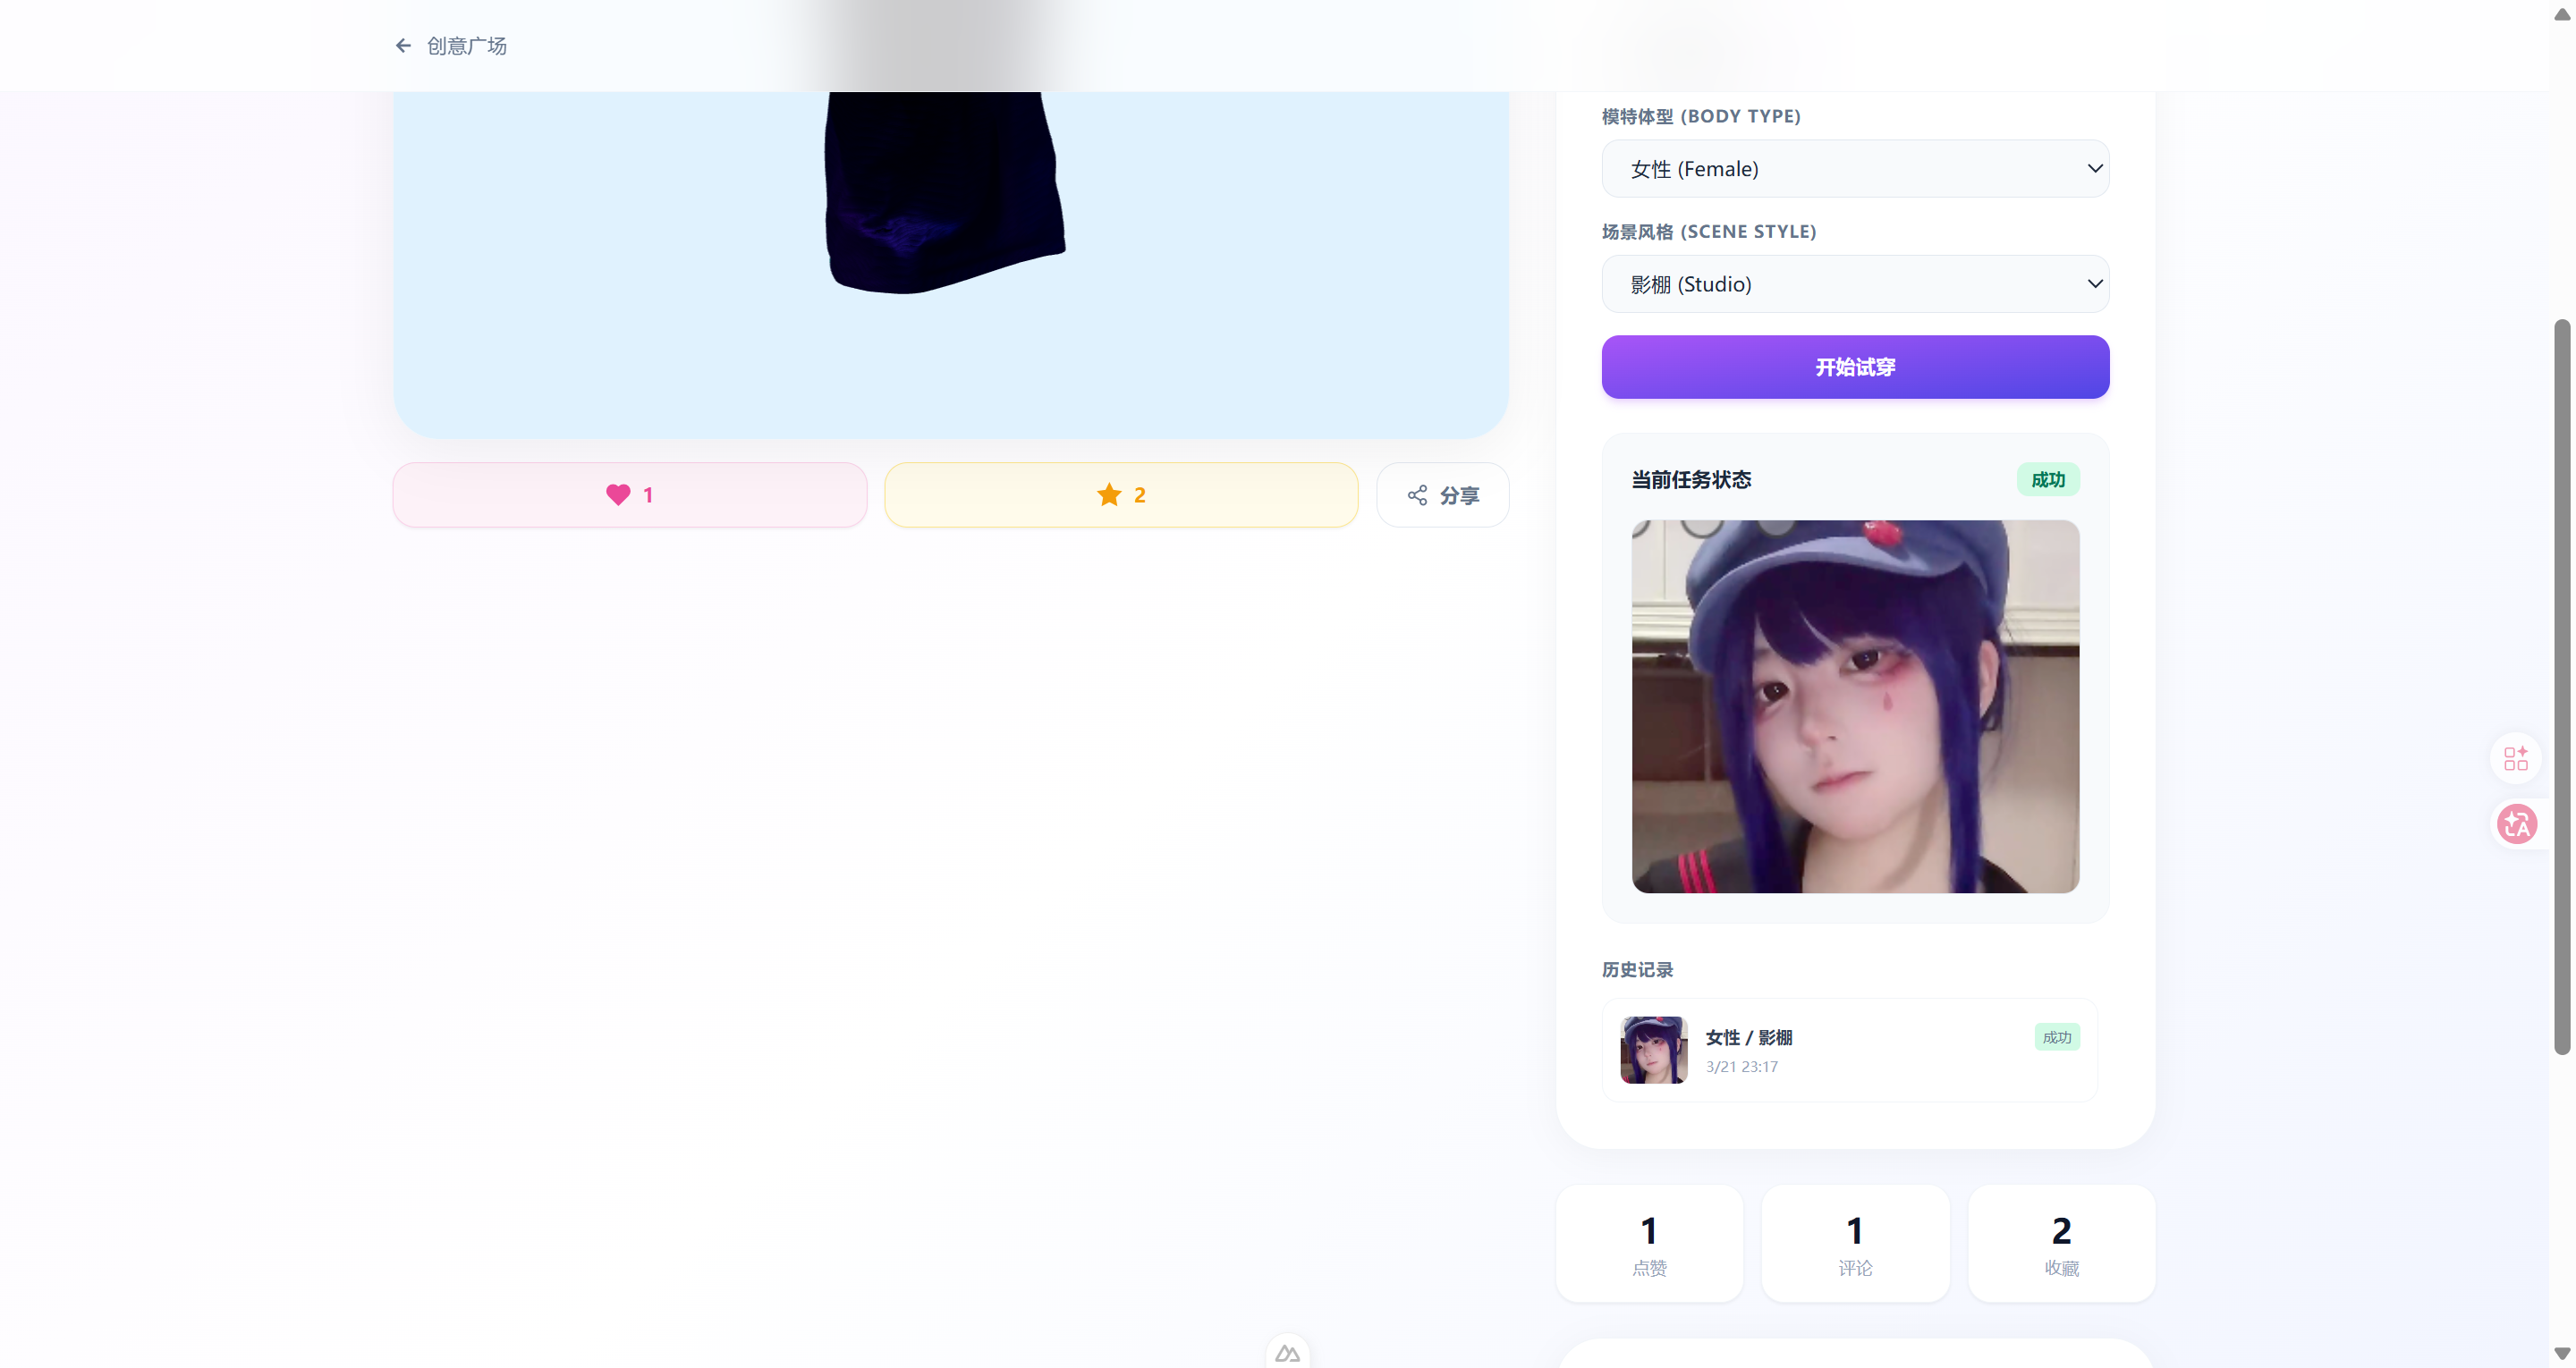
\includegraphics[width=0.85\textwidth]{AI2.png}
	\caption{AI 虚拟试穿生成结果}
	\label{fig:impl-tryon-result}
\end{figure}

\subsection{创意广场模块实现}

创意广场模块面向作品公开展示与社区互动，支持列表浏览、标签筛选、热度排序、点赞、收藏、评论以及关注创作者。前端对应广场首页与作品详情页，后端支持可选登录态访问和缓存加速。创意广场模块接口如表~\ref{tab:api-square} 所示。此部分的核心代码参看附录D

\begin{table}[H]
	\centering
	\caption{创意广场模块接口}
	\label{tab:api-square}
	\renewcommand{\arraystretch}{1.25}
	\setlength{\tabcolsep}{0.2ex}
	\begin{tabularx}{\textwidth}{@{}>{\raggedright\arraybackslash}p{0.26\textwidth} >{\raggedright\arraybackslash}X >{\centering\arraybackslash}p{0.14\textwidth}@{}}
		\toprule
		功能说明 & 接口 API & Http 方法 \\
		\midrule
		广场作品列表 & \texttt{/api/front/square/works} & GET \\
		广场作品详情 & \texttt{/api/front/square/works/:id} & GET \\
		广场标签列表 & \texttt{/api/front/square/tags} & GET \\
		点赞/取消点赞 & \texttt{/api/front/square/works/:id/like} & POST \\
		收藏/取消收藏 & \texttt{/api/front/square/works/:id/favorite} & POST \\
		发表评论 & \texttt{/api/front/square/works/:id/comment} & POST \\
		关注/取消关注作者 & \texttt{/api/front/square/users/:id/follow} & POST \\
		\bottomrule
	\end{tabularx}
\end{table}

该模块实现过程如下：
\begin{enumerate}[label=(\arabic*)]
	\item 仅展示“已发布”状态作品，保证内容质量与流程一致性；
	\item 支持按标签、关键字、热度/趋势进行组合检索；
	\item 未登录用户可浏览，登录用户可返回点赞/收藏状态；
	\item 点赞与收藏使用关联表记录，并同步维护计数字段；
	\item 评论写入评论表，作品评论总数同步更新；
	\item 关注关系写入 \texttt{user\_follows} 表，并同步更新用户的 \texttt{followers\_count}/\texttt{following\_count} 计数；
	\item 为提升访问性能，列表/详情/标签使用 Redis 缓存；
	\item 交互动作触发缓存失效，保证数据实时性与一致性，界面如图~\ref{fig:impl-square}所示。
\end{enumerate}

\begin{figure}[H]
	\centering
	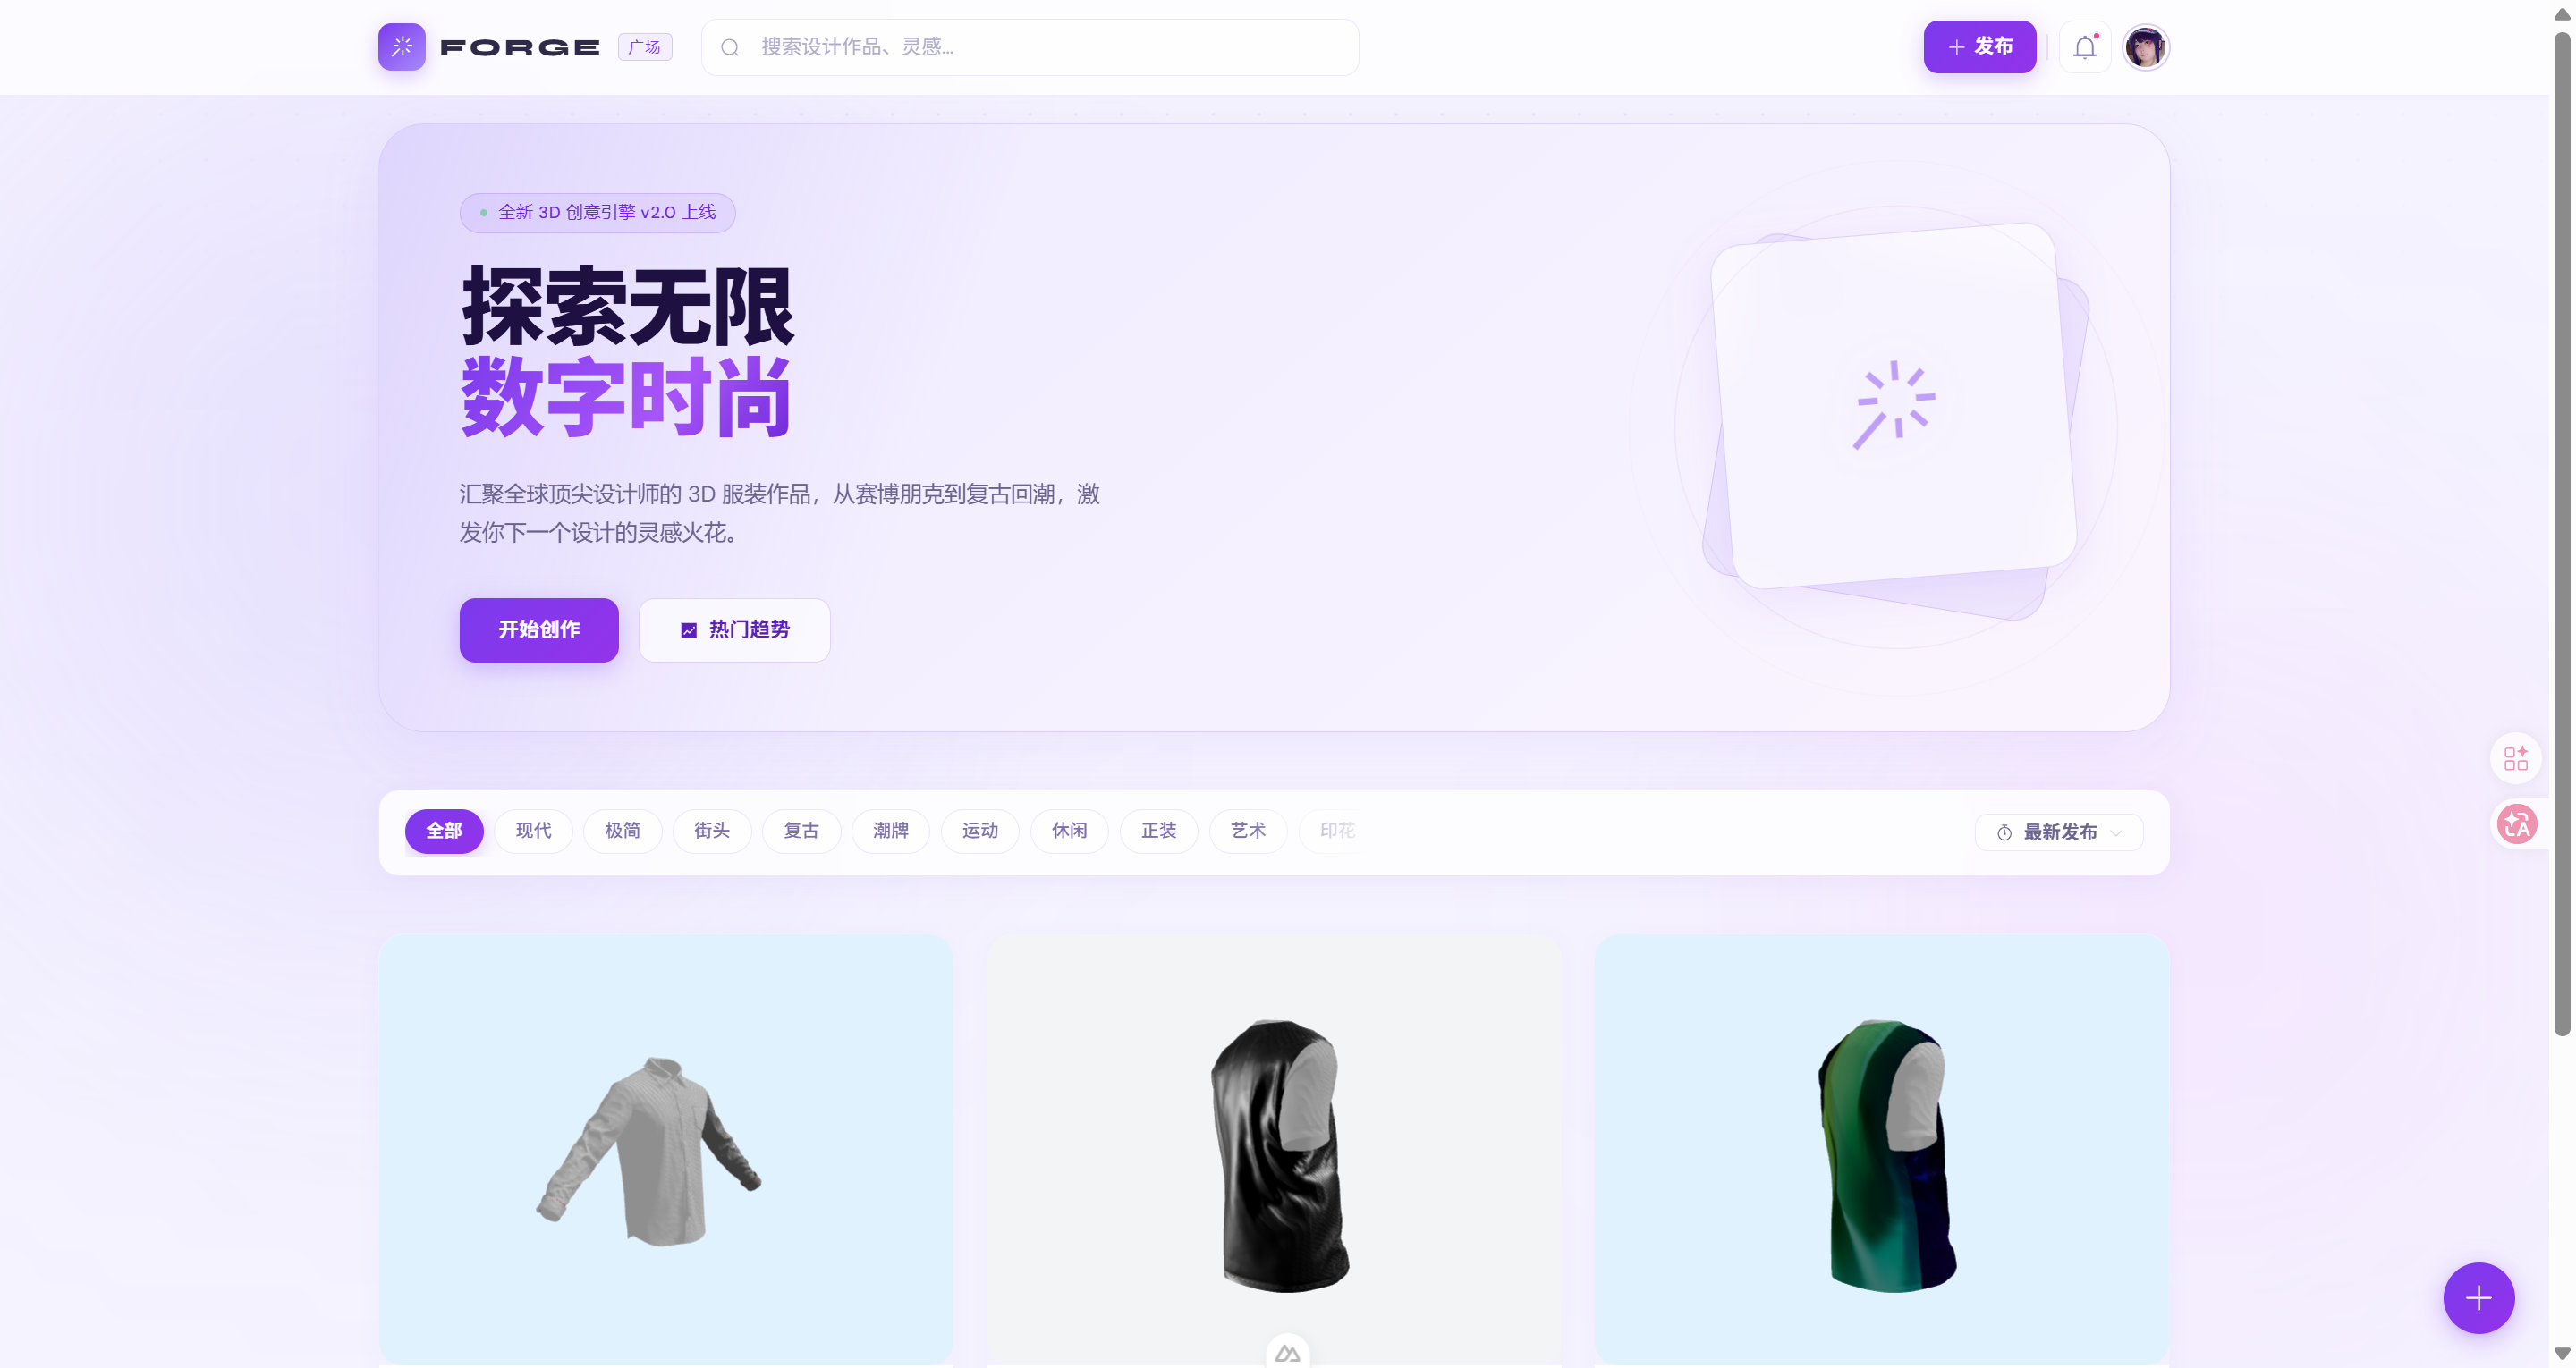
\includegraphics[width=0.85\textwidth]{square.png}
	\caption{创意广场}
	\label{fig:impl-square}
\end{figure}

\subsection{作品管理模块实现}

作品管理模块负责前台用户对个人作品的全生命周期管理，包括创建、编辑、提审、查看详情、下架和删除，并与审核流程、试穿流程联动。作品管理模块接口如表~\ref{tab:api-work} 所示。此部分的核心代码参看附录E

\begin{table}[H]
	\centering
	\caption{作品管理模块接口}
	\label{tab:api-work}
	\renewcommand{\arraystretch}{1.25}
	\setlength{\tabcolsep}{0.2ex}
	\begin{tabularx}{\textwidth}{@{}>{\raggedright\arraybackslash}p{0.26\textwidth} >{\raggedright\arraybackslash}X >{\centering\arraybackslash}p{0.14\textwidth}@{}}
		\toprule
		功能说明 & 接口 API & Http 方法 \\
		\midrule
		作品列表 & \texttt{/api/front/works} & GET \\
		作品详情 & \texttt{/api/front/works/:id} & GET \\
		创建作品 & \texttt{/api/front/works} & POST \\
		修改作品 & \texttt{/api/front/works/:id} & POST \\
		提交审核 & \texttt{/api/front/works/:id/submit} & POST \\
		下架作品 & \texttt{/api/front/works/:id/unpublish} & POST \\
		删除作品 & \texttt{/api/front/works/:id} & DELETE \\
		\bottomrule
	\end{tabularx}
\end{table}

该模块实现过程如下：
\begin{enumerate}[label=(\arabic*)]
	\item 前端“我的作品”页分页拉取作品列表；
	\item 用户创建作品后默认进入草稿态；
	\item 编辑接口按状态机控制可编辑范围；
	\item 提交审核后状态转为“已提交”，等待管理员审核；
	\item 详情页聚合展示作品信息、审核记录与试穿历史；
	\item 下架接口将发布作品恢复为草稿态，支持继续修改；
	\item 删除接口限制审核中/已发布作品，避免业务流程异常，界面如图~\ref{fig:impl-mywork}所示。
\end{enumerate}

\begin{figure}[H]
	\centering
	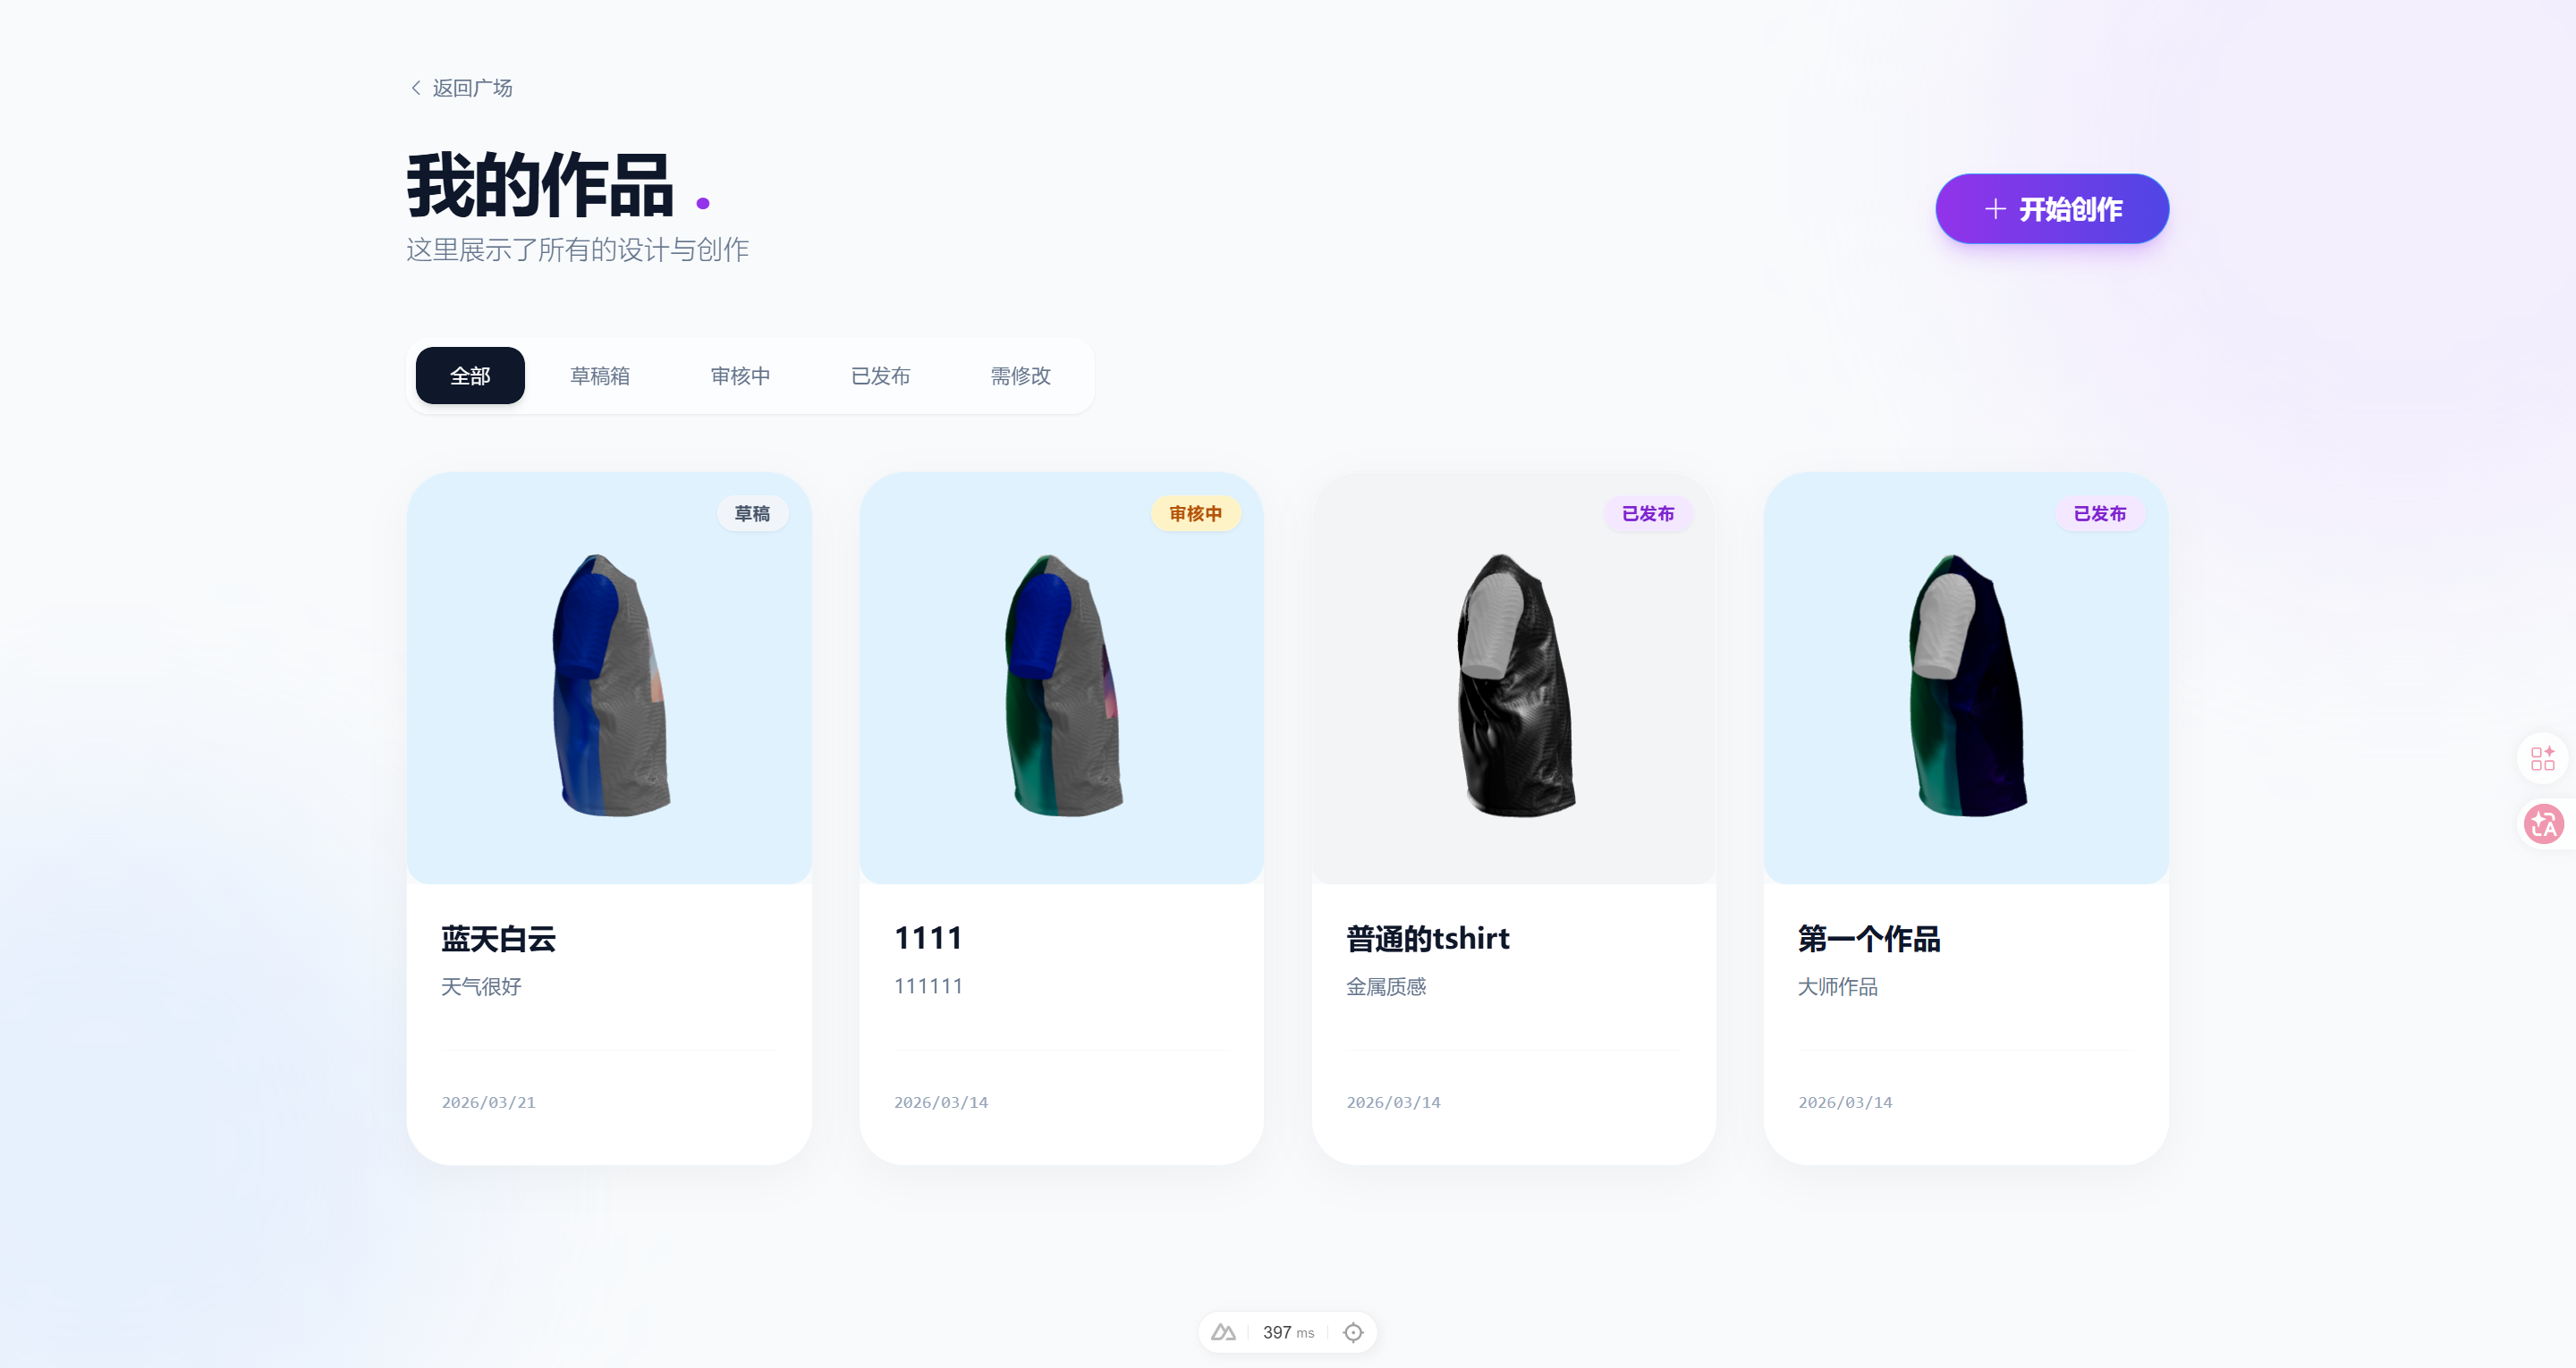
\includegraphics[width=0.85\textwidth]{mywork.png}
	\caption{作品管理}
	\label{fig:impl-mywork}
\end{figure}

\subsection{后台管理模块实现}

后台管理模块用于管理员对平台资源进行统一治理，涵盖管理员登录、用户管理、模型管理和作品审核。后端通过“认证中间件 + 管理员权限中间件”实现访问控制。后台管理模块接口如表~\ref{tab:api-admin} 所示。此部分的核心代码参看附录F

\begin{table}[H]
	\centering
	\caption{后台管理模块接口}
	\label{tab:api-admin}
	\renewcommand{\arraystretch}{1.25}
	\setlength{\tabcolsep}{0.2ex}
	\begin{tabularx}{\textwidth}{@{}>{\raggedright\arraybackslash}p{0.36\textwidth} >{\raggedright\arraybackslash}X >{\centering\arraybackslash}p{0.16\textwidth}@{}}
		\toprule
		功能说明 & 接口 API & Http 方法 \\
		\midrule
		管理员登录 & \texttt{/api/admin/login} & POST \\
		用户管理（查/增/改/删） & \texttt{/api/admin/users} 及子路径 & GET/POST/DELETE \\
		用户密码重置 & \texttt{/api/admin/users/:id/password} & POST \\
		模型管理（查/增/改/删） & \texttt{/api/admin/models} 及子路径 & GET/POST/DELETE \\
		模型文件上传 & \texttt{/api/admin/models/upload} & POST \\
		作品审核列表 & \texttt{/api/admin/works} & GET \\
		审核处理 & \texttt{/api/admin/works/:id/review} & POST \\
		\bottomrule
	\end{tabularx}
\end{table}

该模块实现过程如下：
\begin{enumerate}[label=(\arabic*)]
	\item 管理员登录后校验角色为管理员角色；
	\item 后台接口统一要求 JWT 且通过管理员权限校验；
	\item 用户管理支持分页检索、角色维护、密码重置；
	\item 模型管理支持文件上传至对象存储并同步写入数据库；
	\item 作品审核仅允许“已提交”状态进入审核流程；
	\item 审核通过将作品发布，审核驳回需填写原因并返回驳回态；
	\item 前端管理端根据审核结果刷新待审列表与历史记录，界面如图~\ref{fig:impl-admin-user}、图~\ref{fig:impl-admin-review}、图~\ref{fig:impl-admin-model}所示。
\end{enumerate}

\begin{figure}[H]
	\centering
	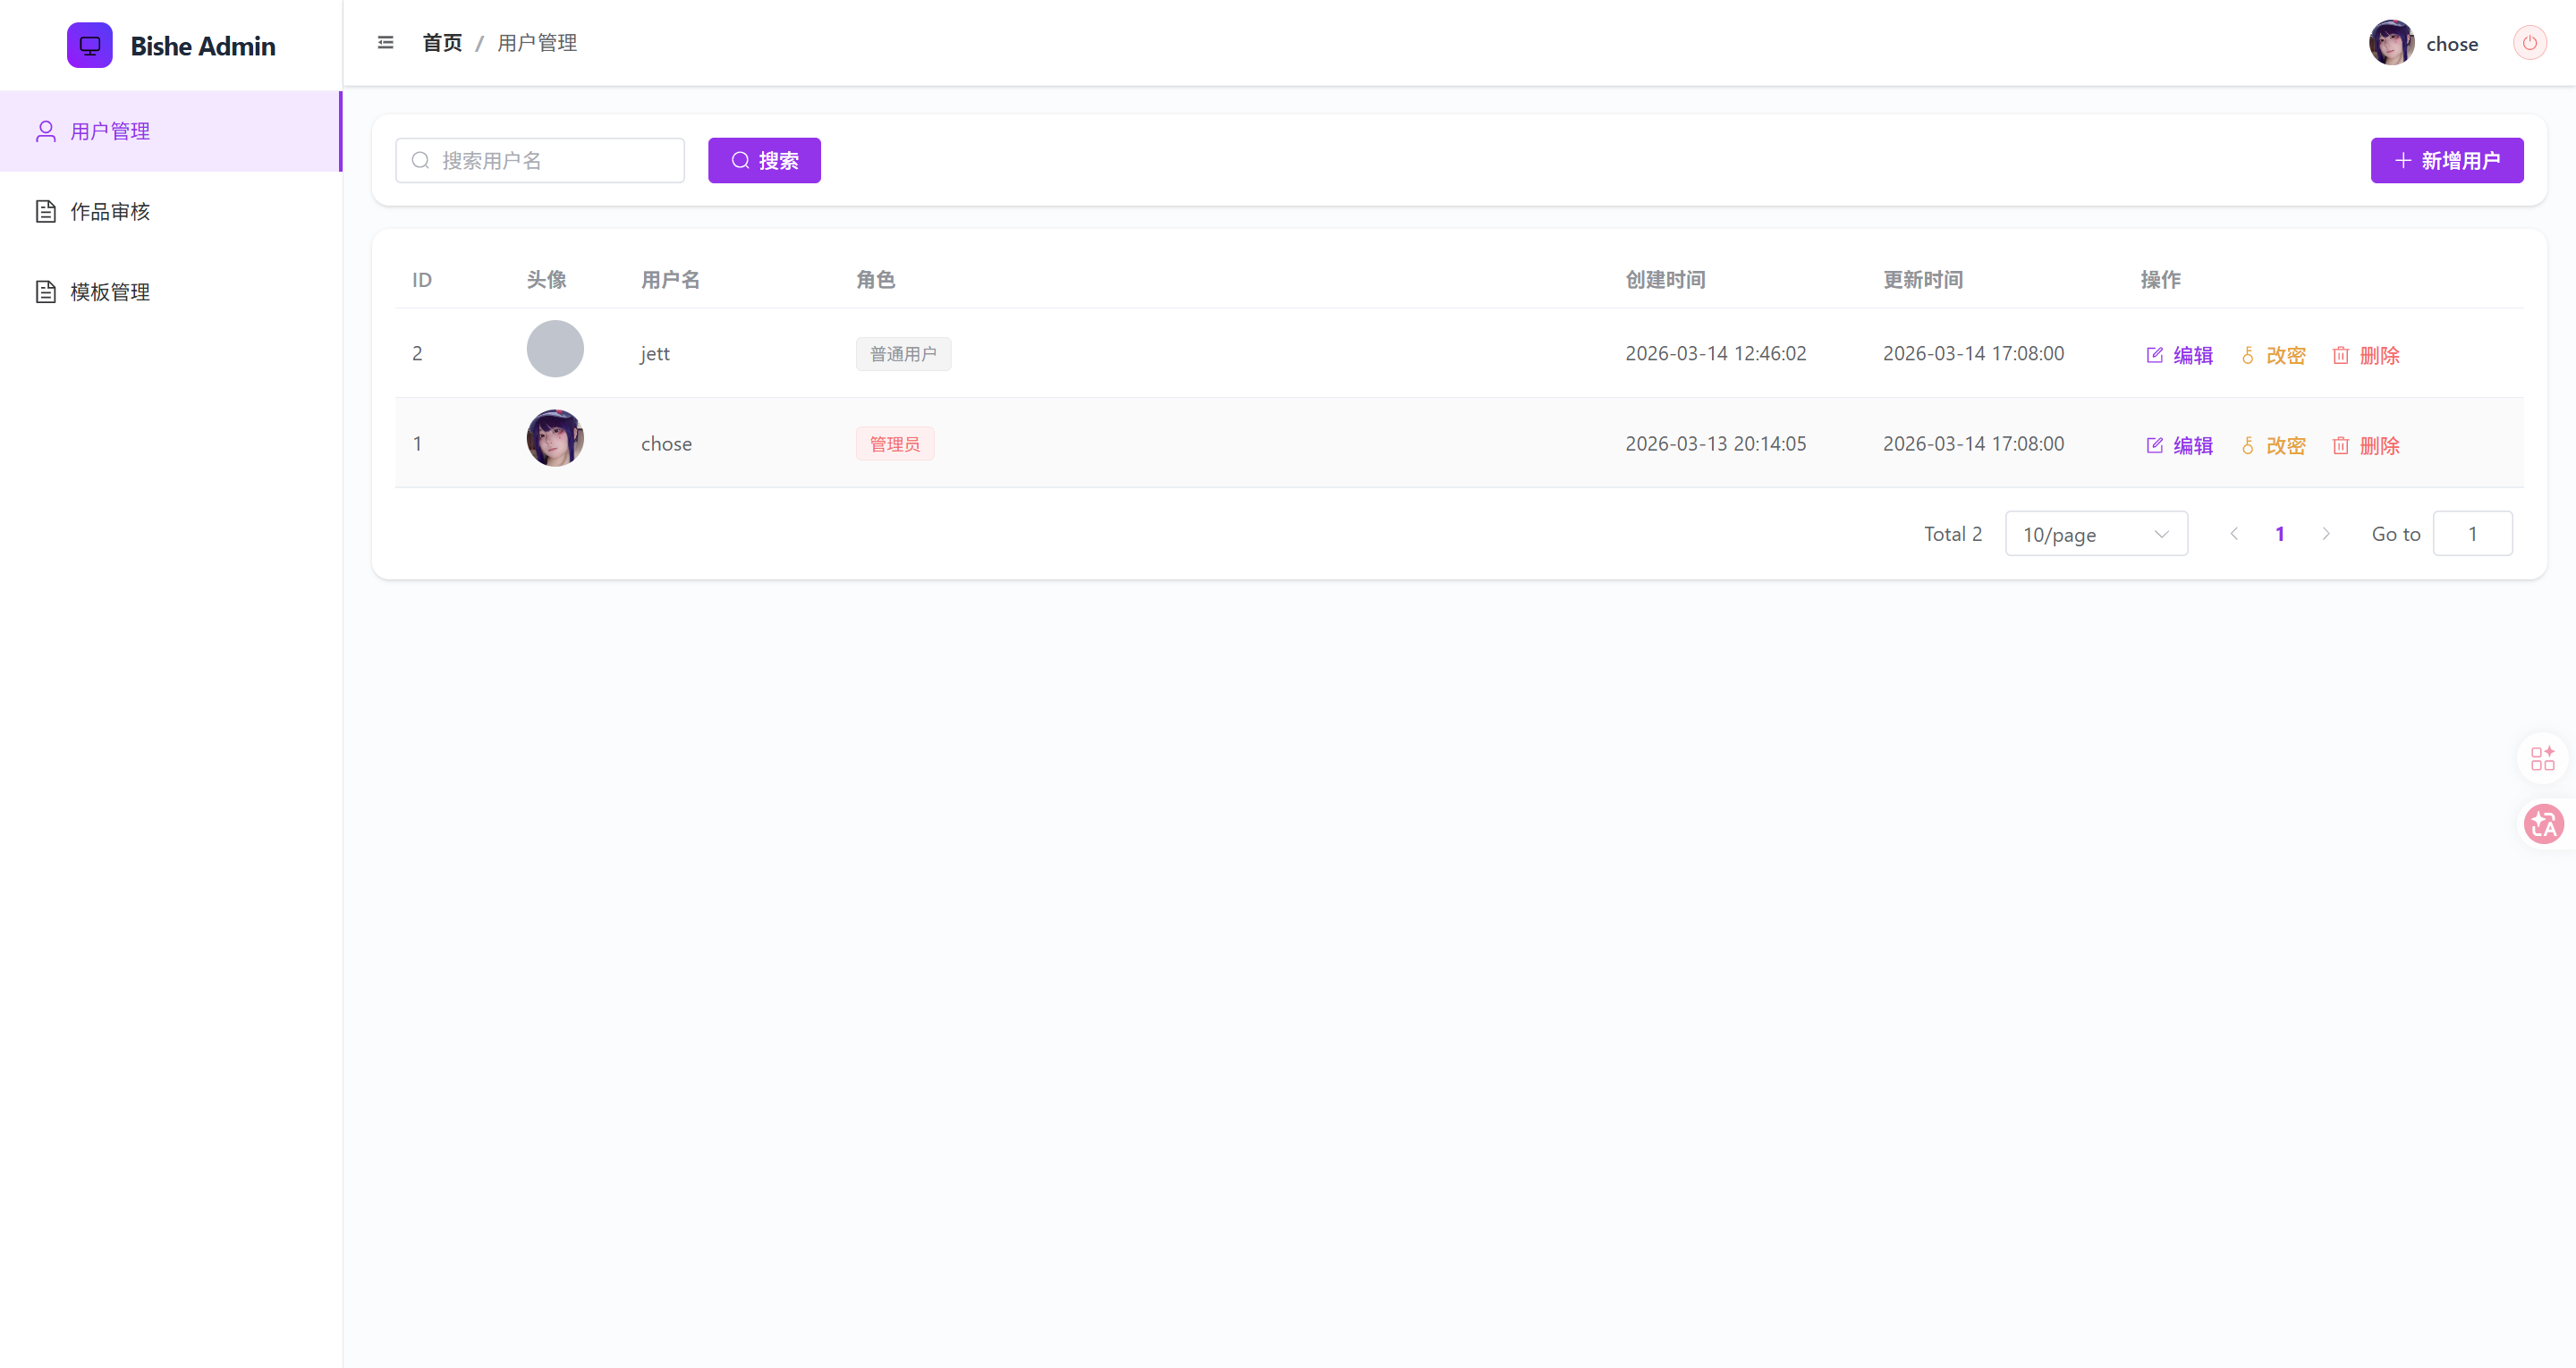
\includegraphics[width=0.85\textwidth]{admin1.png}
	\caption{用户管理}
	\label{fig:impl-admin-user}
\end{figure}

\begin{figure}[H]
	\centering
	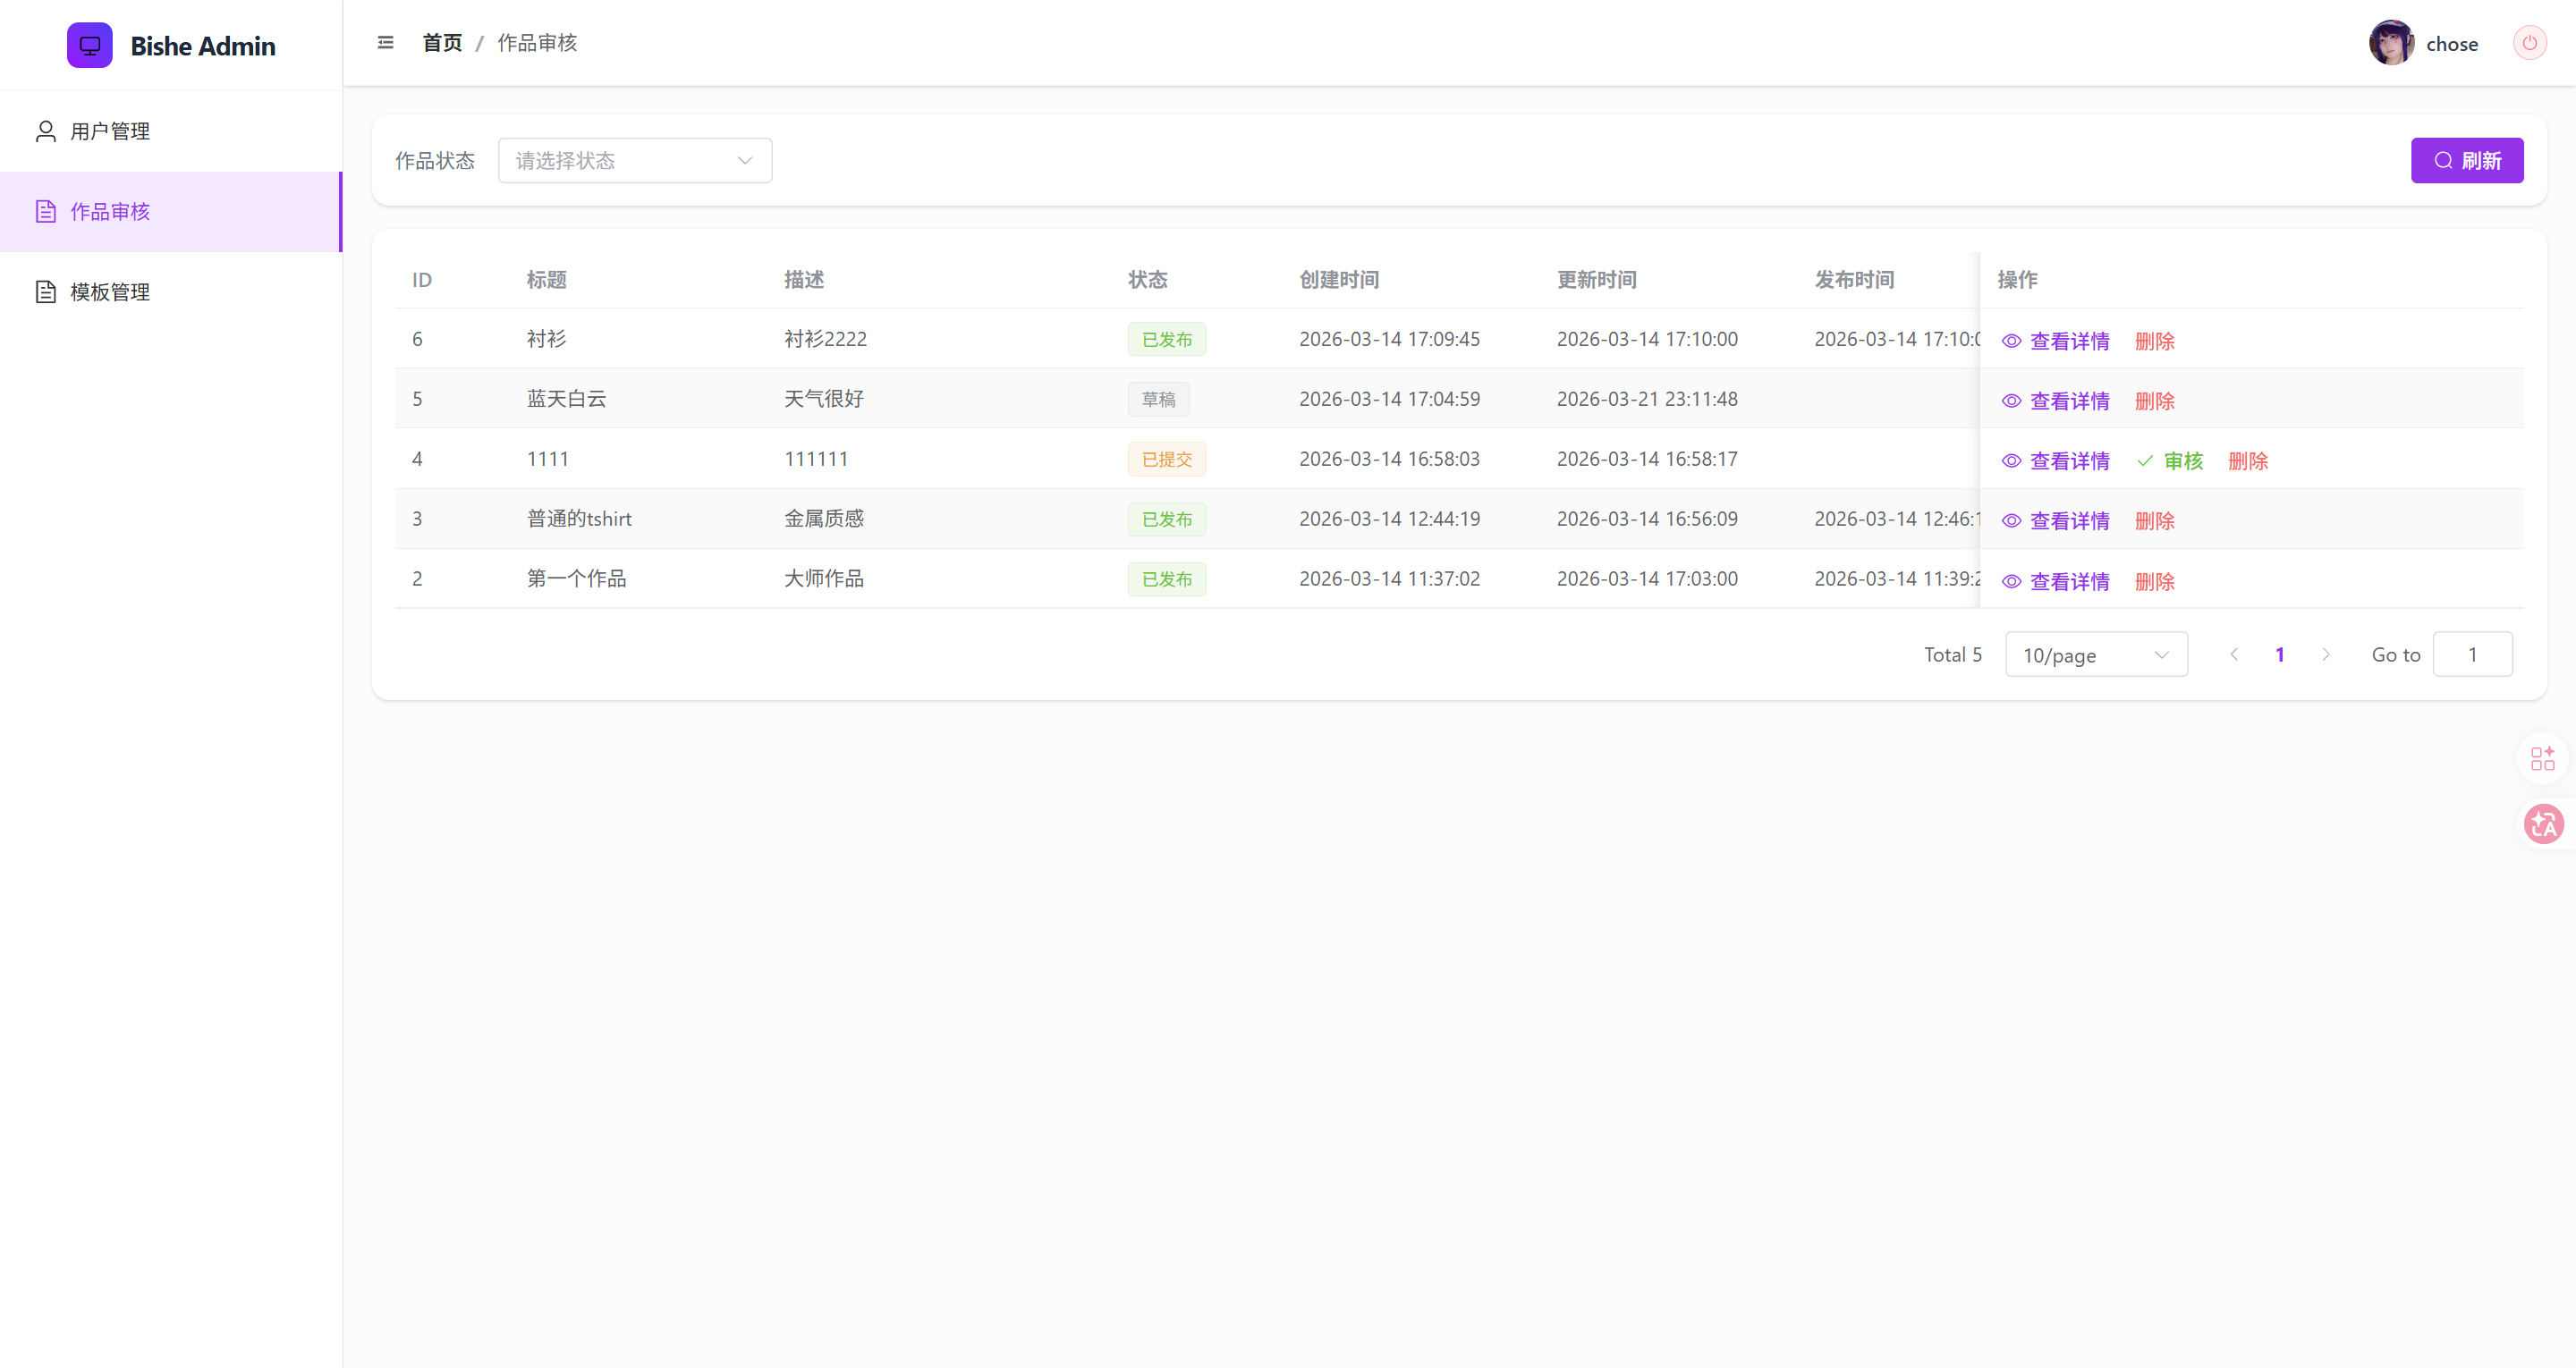
\includegraphics[width=0.85\textwidth]{admin2.png}
	\caption{作品审核}
	\label{fig:impl-admin-review}
\end{figure}

\begin{figure}[H]
	\centering
	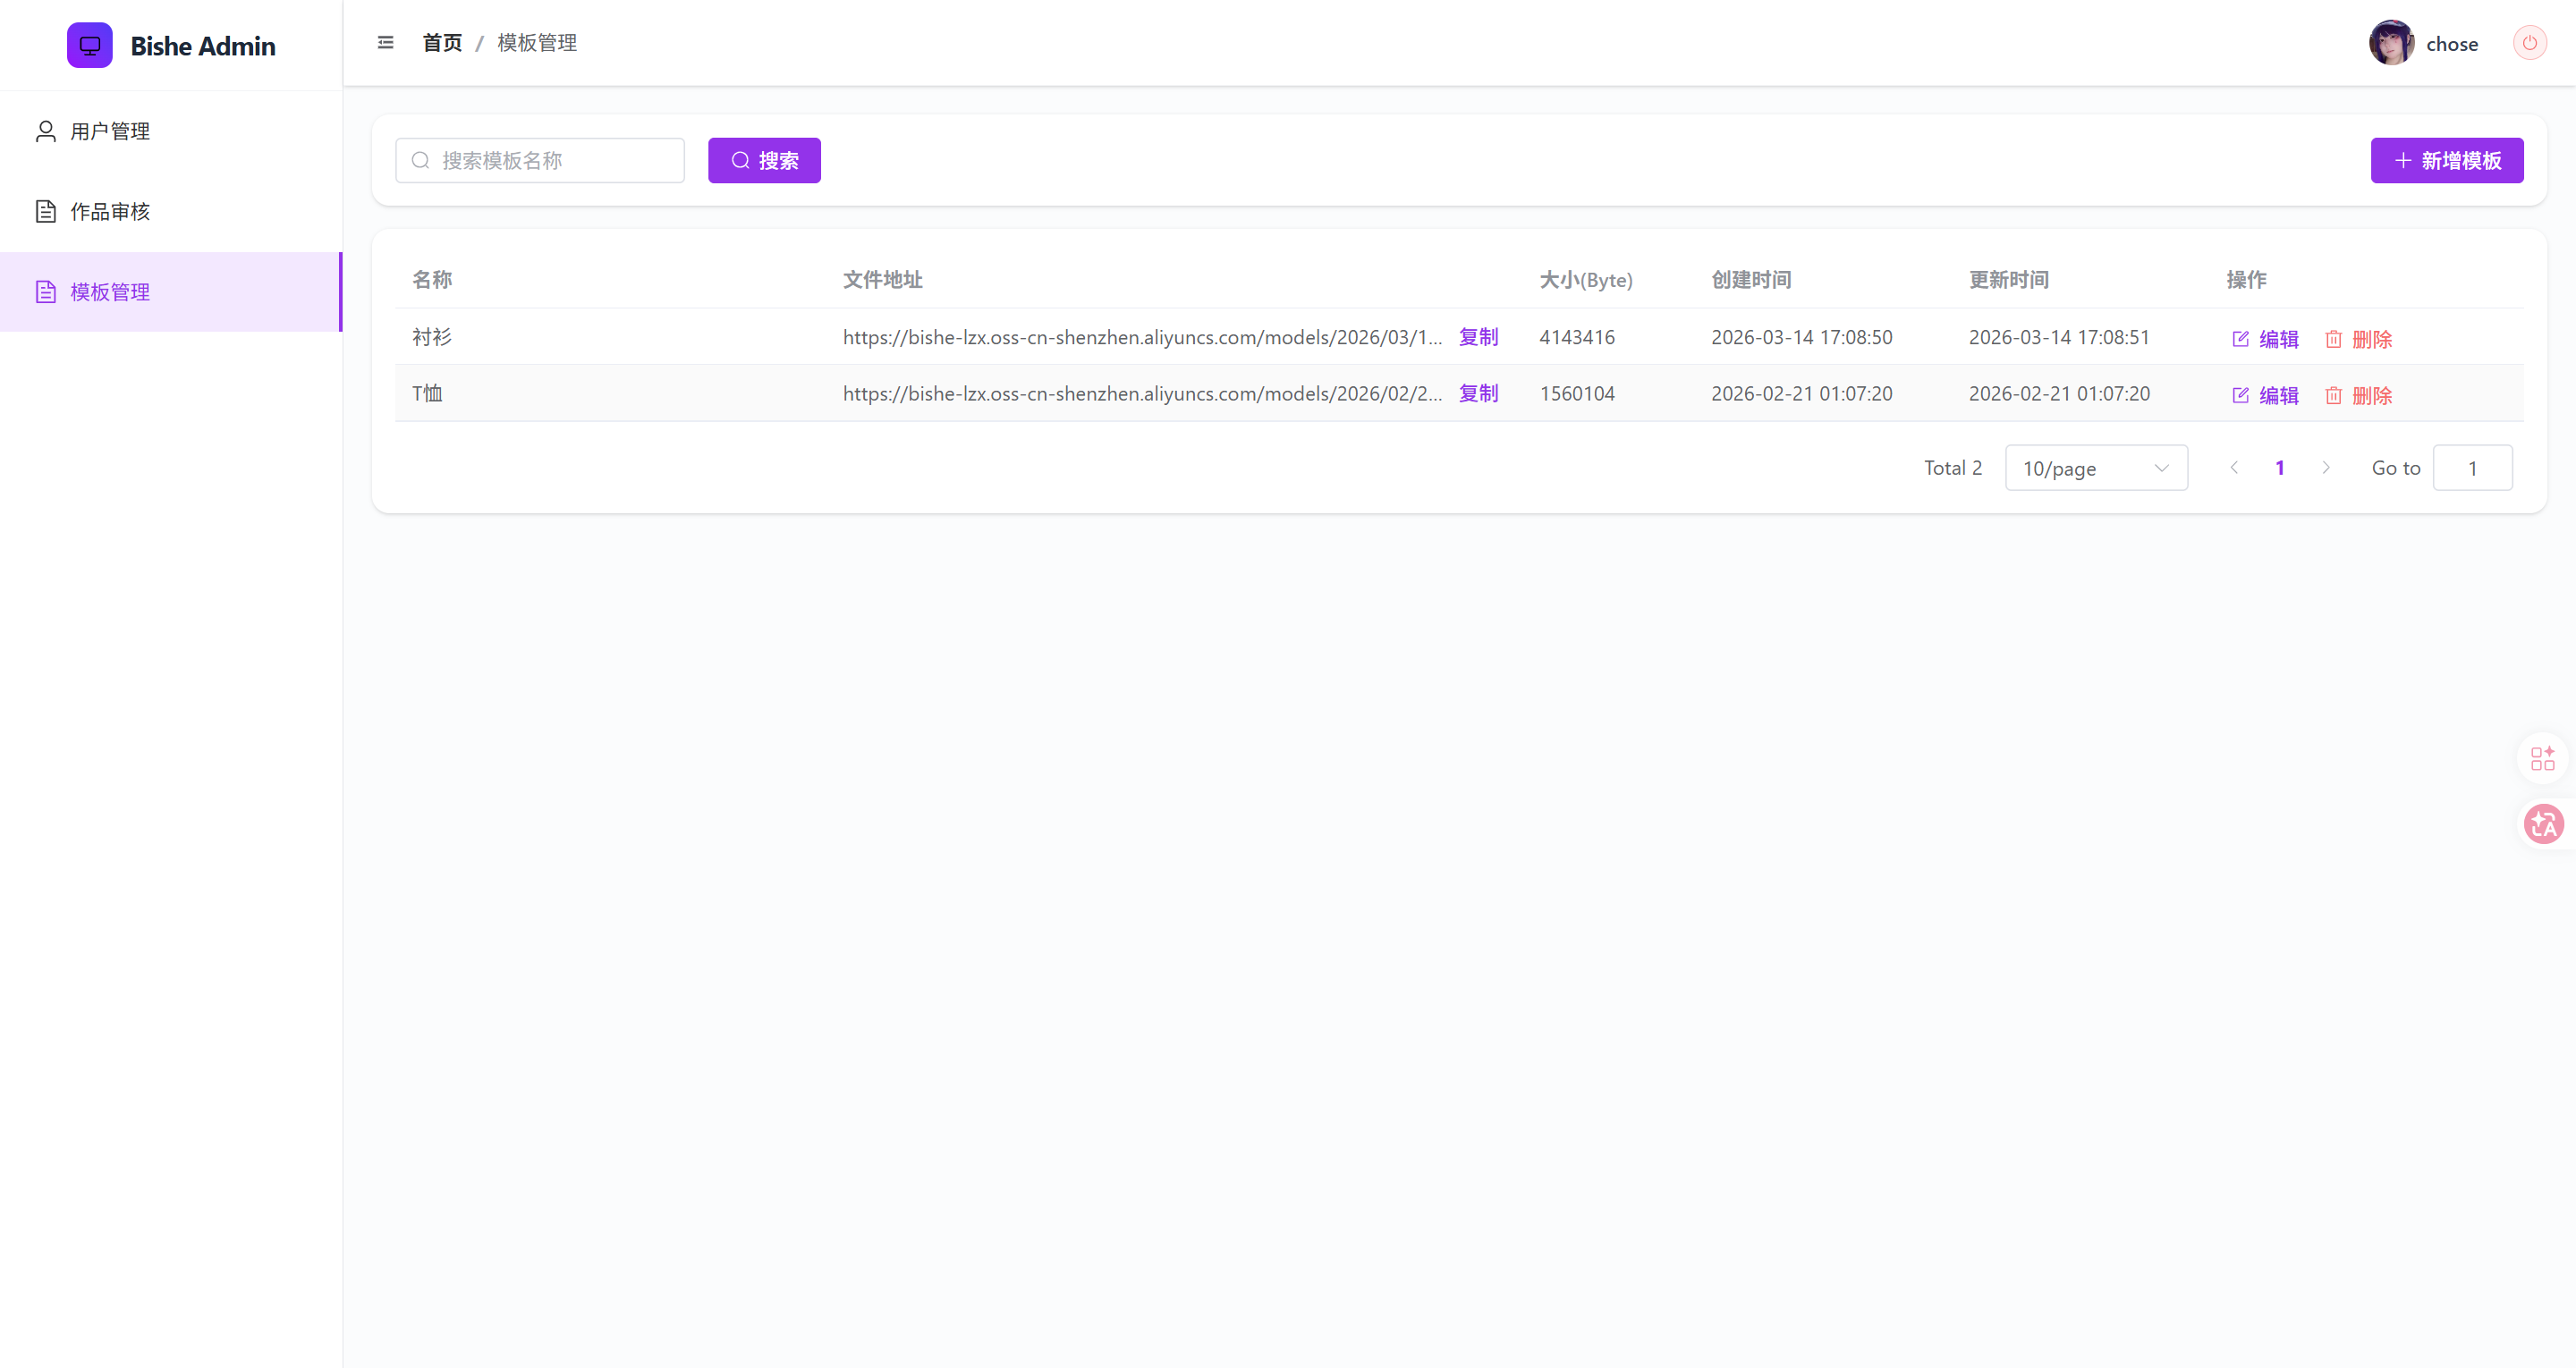
\includegraphics[width=0.85\textwidth]{admin3.png}
	\caption{模型管理}
	\label{fig:impl-admin-model}
\end{figure}

\chapter{系统测试}

本章主要对系统的核心功能进行黑盒测试，采用“按模块设计用例 + 关键路径优先”的方式覆盖主流程、边界场景与异常处理。测试过程中重点关注：功能正确性、交互完整性、输入校验、权限控制、错误提示与数据一致性。

\section{功能测试}

\subsection{用户模块测试}

用户模块主要覆盖注册登录、个人信息维护、账号安全与会话状态等功能。

\subsubsection{注册与登录}

测试用例如表~\ref{tab:testcase-register-login}所示。

\begin{table}[H]
	\centering
	\caption{注册与登录测试用例}
	\label{tab:testcase-register-login}
	\renewcommand{\arraystretch}{1.25}
	\setlength{\tabcolsep}{0.2ex}
	\begin{tabularx}{\textwidth}{@{}>{\raggedright\arraybackslash}p{0.12\textwidth} >{\raggedright\arraybackslash}p{0.22\textwidth} >{\raggedright\arraybackslash}X >{\raggedright\arraybackslash}X@{}}
		\toprule
		\textbf{\mbox{用例ID}} & \textbf{\mbox{前置条件}} & \textbf{\mbox{测试步骤}} & \textbf{\mbox{期望结果}} \\
		\midrule
		\mbox{001} & 未登录状态；用户名为未注册状态。 & 1. 进入注册页，输入合法信息并提交；\newline 2. 注册成功后返回登录页，使用新账号登录；\newline 3. 退出登录后再次登录，验证会话恢复与登录态保持逻辑。 & 1. 注册信息校验正确（必填项提示明确、格式错误提示准确）；\newline 2. 注册成功后账号可正常登录；登录失败时提示原因（密码错误/账号不存在等）；\newline 3. 登录后进入正确的首页/个人中心，用户信息与权限展示正常。 \\
		\bottomrule
	\end{tabularx}
\end{table}

测试结果与期望一致：登录失败时能够给出明确原因提示；注册成功后可正常登录并保持会话状态。结果如图~\ref{fig:test-login-fail}和图~\ref{fig:test-login-success}所示。

\begin{figure}[H]
	\centering
	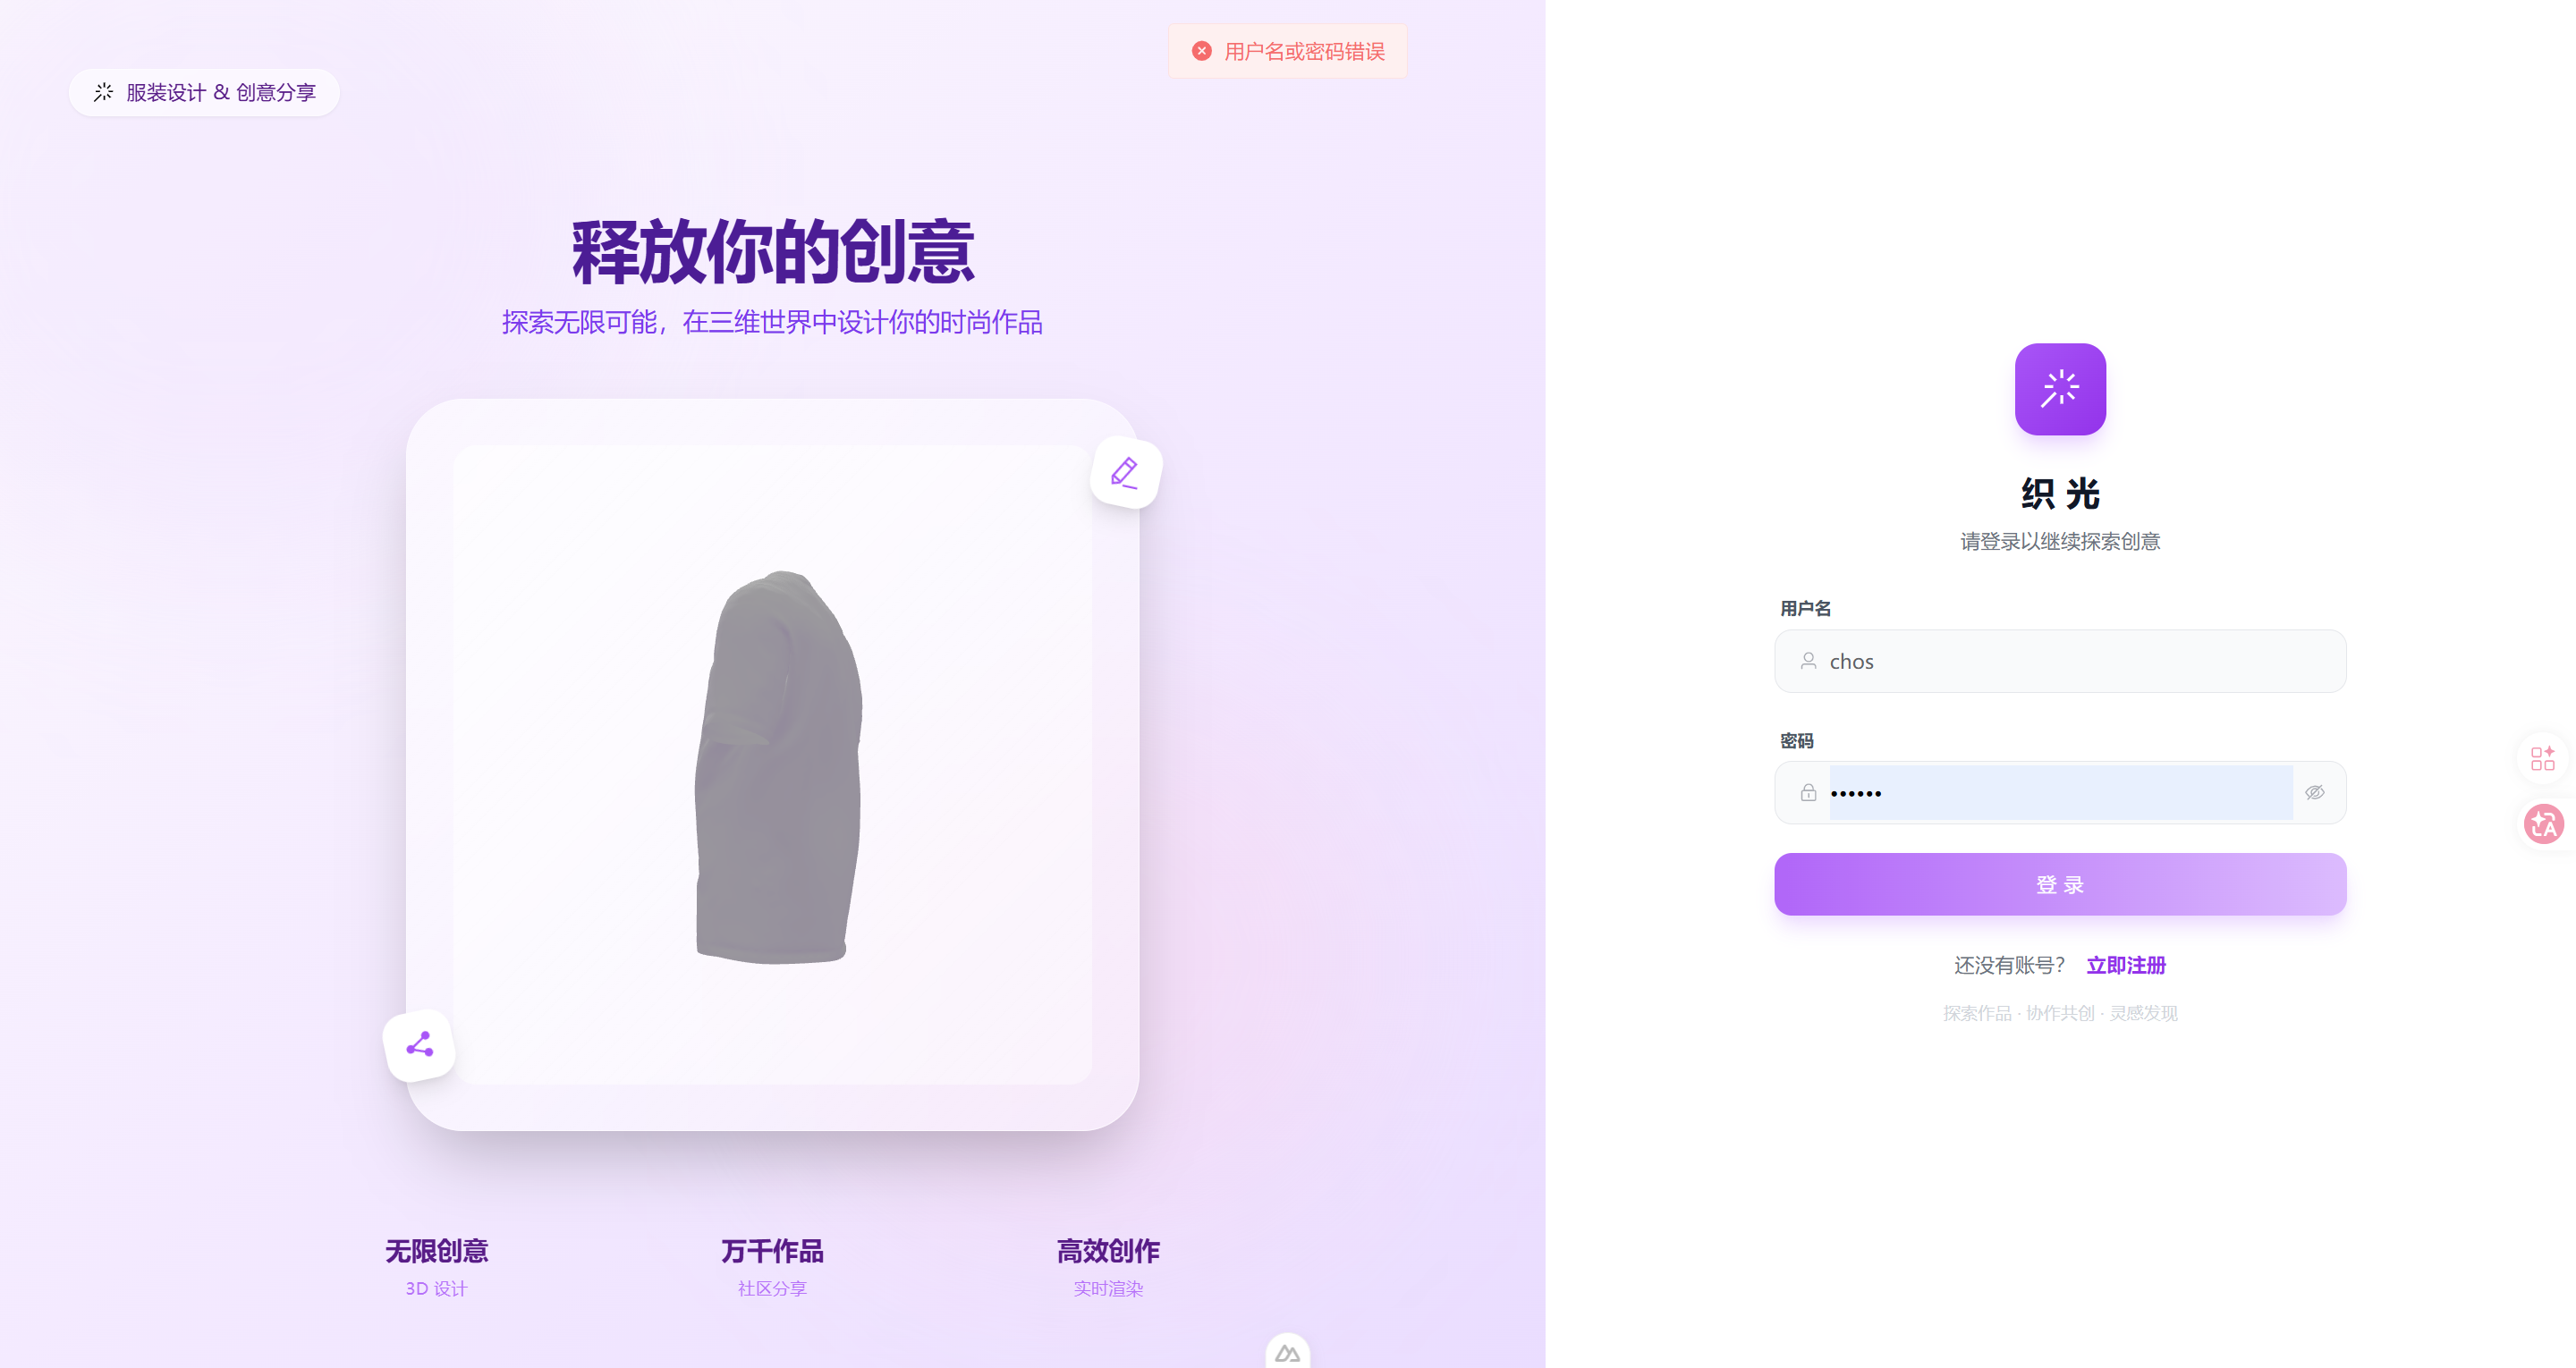
\includegraphics[width=0.85\textwidth]{test1}
	\caption{注册与登录失败提示}
	\label{fig:test-login-fail}
\end{figure}

\begin{figure}[H]
	\centering
	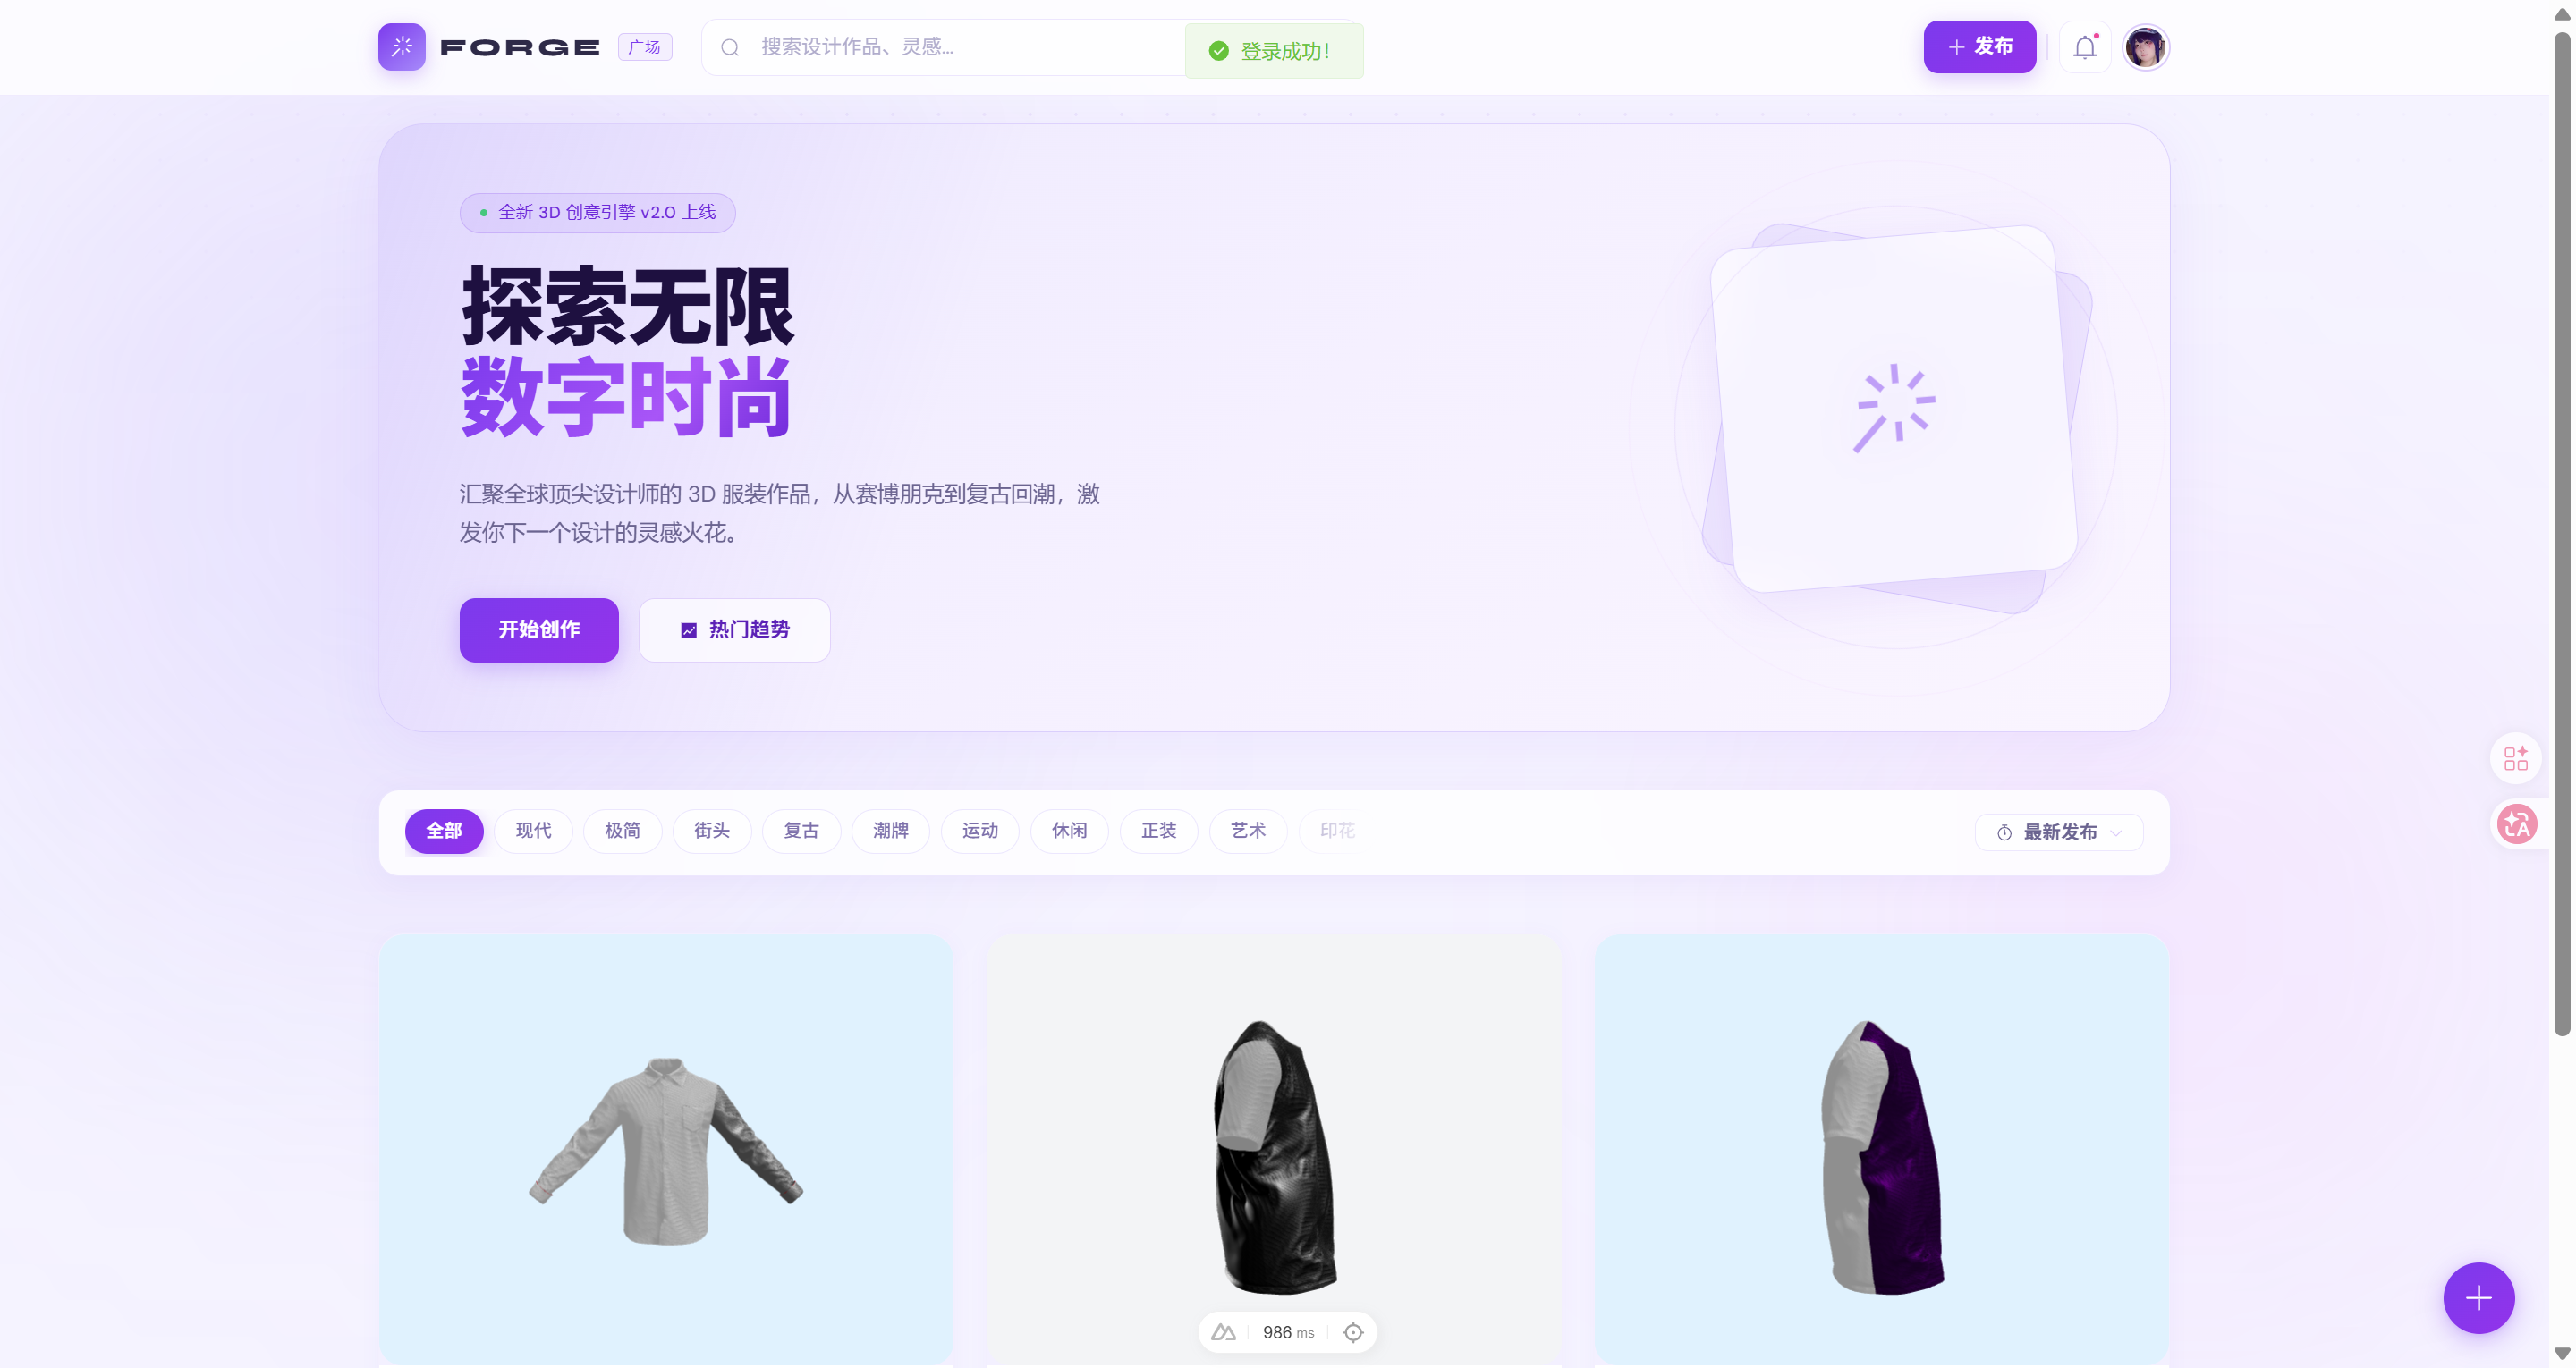
\includegraphics[width=0.85\textwidth]{test2}
	\caption{注册与登录成功页面}
	\label{fig:test-login-success}
\end{figure}

\subsubsection{个人信息与资料维护}

测试用例如表~\ref{tab:testcase-profile}所示。

\begin{table}[H]
	\centering
	\caption{个人信息与资料维护测试用例}
	\label{tab:testcase-profile}
	\renewcommand{\arraystretch}{1.25}
	\setlength{\tabcolsep}{0.2ex}
	\begin{tabularx}{\textwidth}{@{}>{\raggedright\arraybackslash}p{0.12\textwidth} >{\raggedright\arraybackslash}p{0.22\textwidth} >{\raggedright\arraybackslash}X >{\raggedright\arraybackslash}X@{}}
		\toprule
		\textbf{\mbox{用例ID}} & \textbf{\mbox{前置条件}} & \textbf{\mbox{测试步骤}} & \textbf{\mbox{期望结果}} \\
		\midrule
		\mbox{002} & 已登录。 & 1. 进入个人中心，修改昵称、头像、密码等资料并保存；\newline 2. 刷新页面或重新登录，检查资料是否持久化；\newline 3. 测试修改密码是否生效；\newline 4. 退出登录，验证会话失效与受限资源访问。 & 1. 保存后即时生效且刷新后不丢失；\newline 2. 对不合法输入进行拦截或提示，避免写入异常数据；\newline 3. 退出登录后 token/session 失效，访问受保护页面会被拦截并重定向到登录页。 \\
		\bottomrule
	\end{tabularx}
\end{table}

测试结果与期望一致：个人资料修改保存后可正确回显且持久化；密码修改校验与生效正常；退出登录后受保护资源访问会被拦截并重定向登录。结果如图~\ref{fig:test-profile}和图~\ref{fig:test-password-check}所示。

\begin{figure}[H]
	\centering
	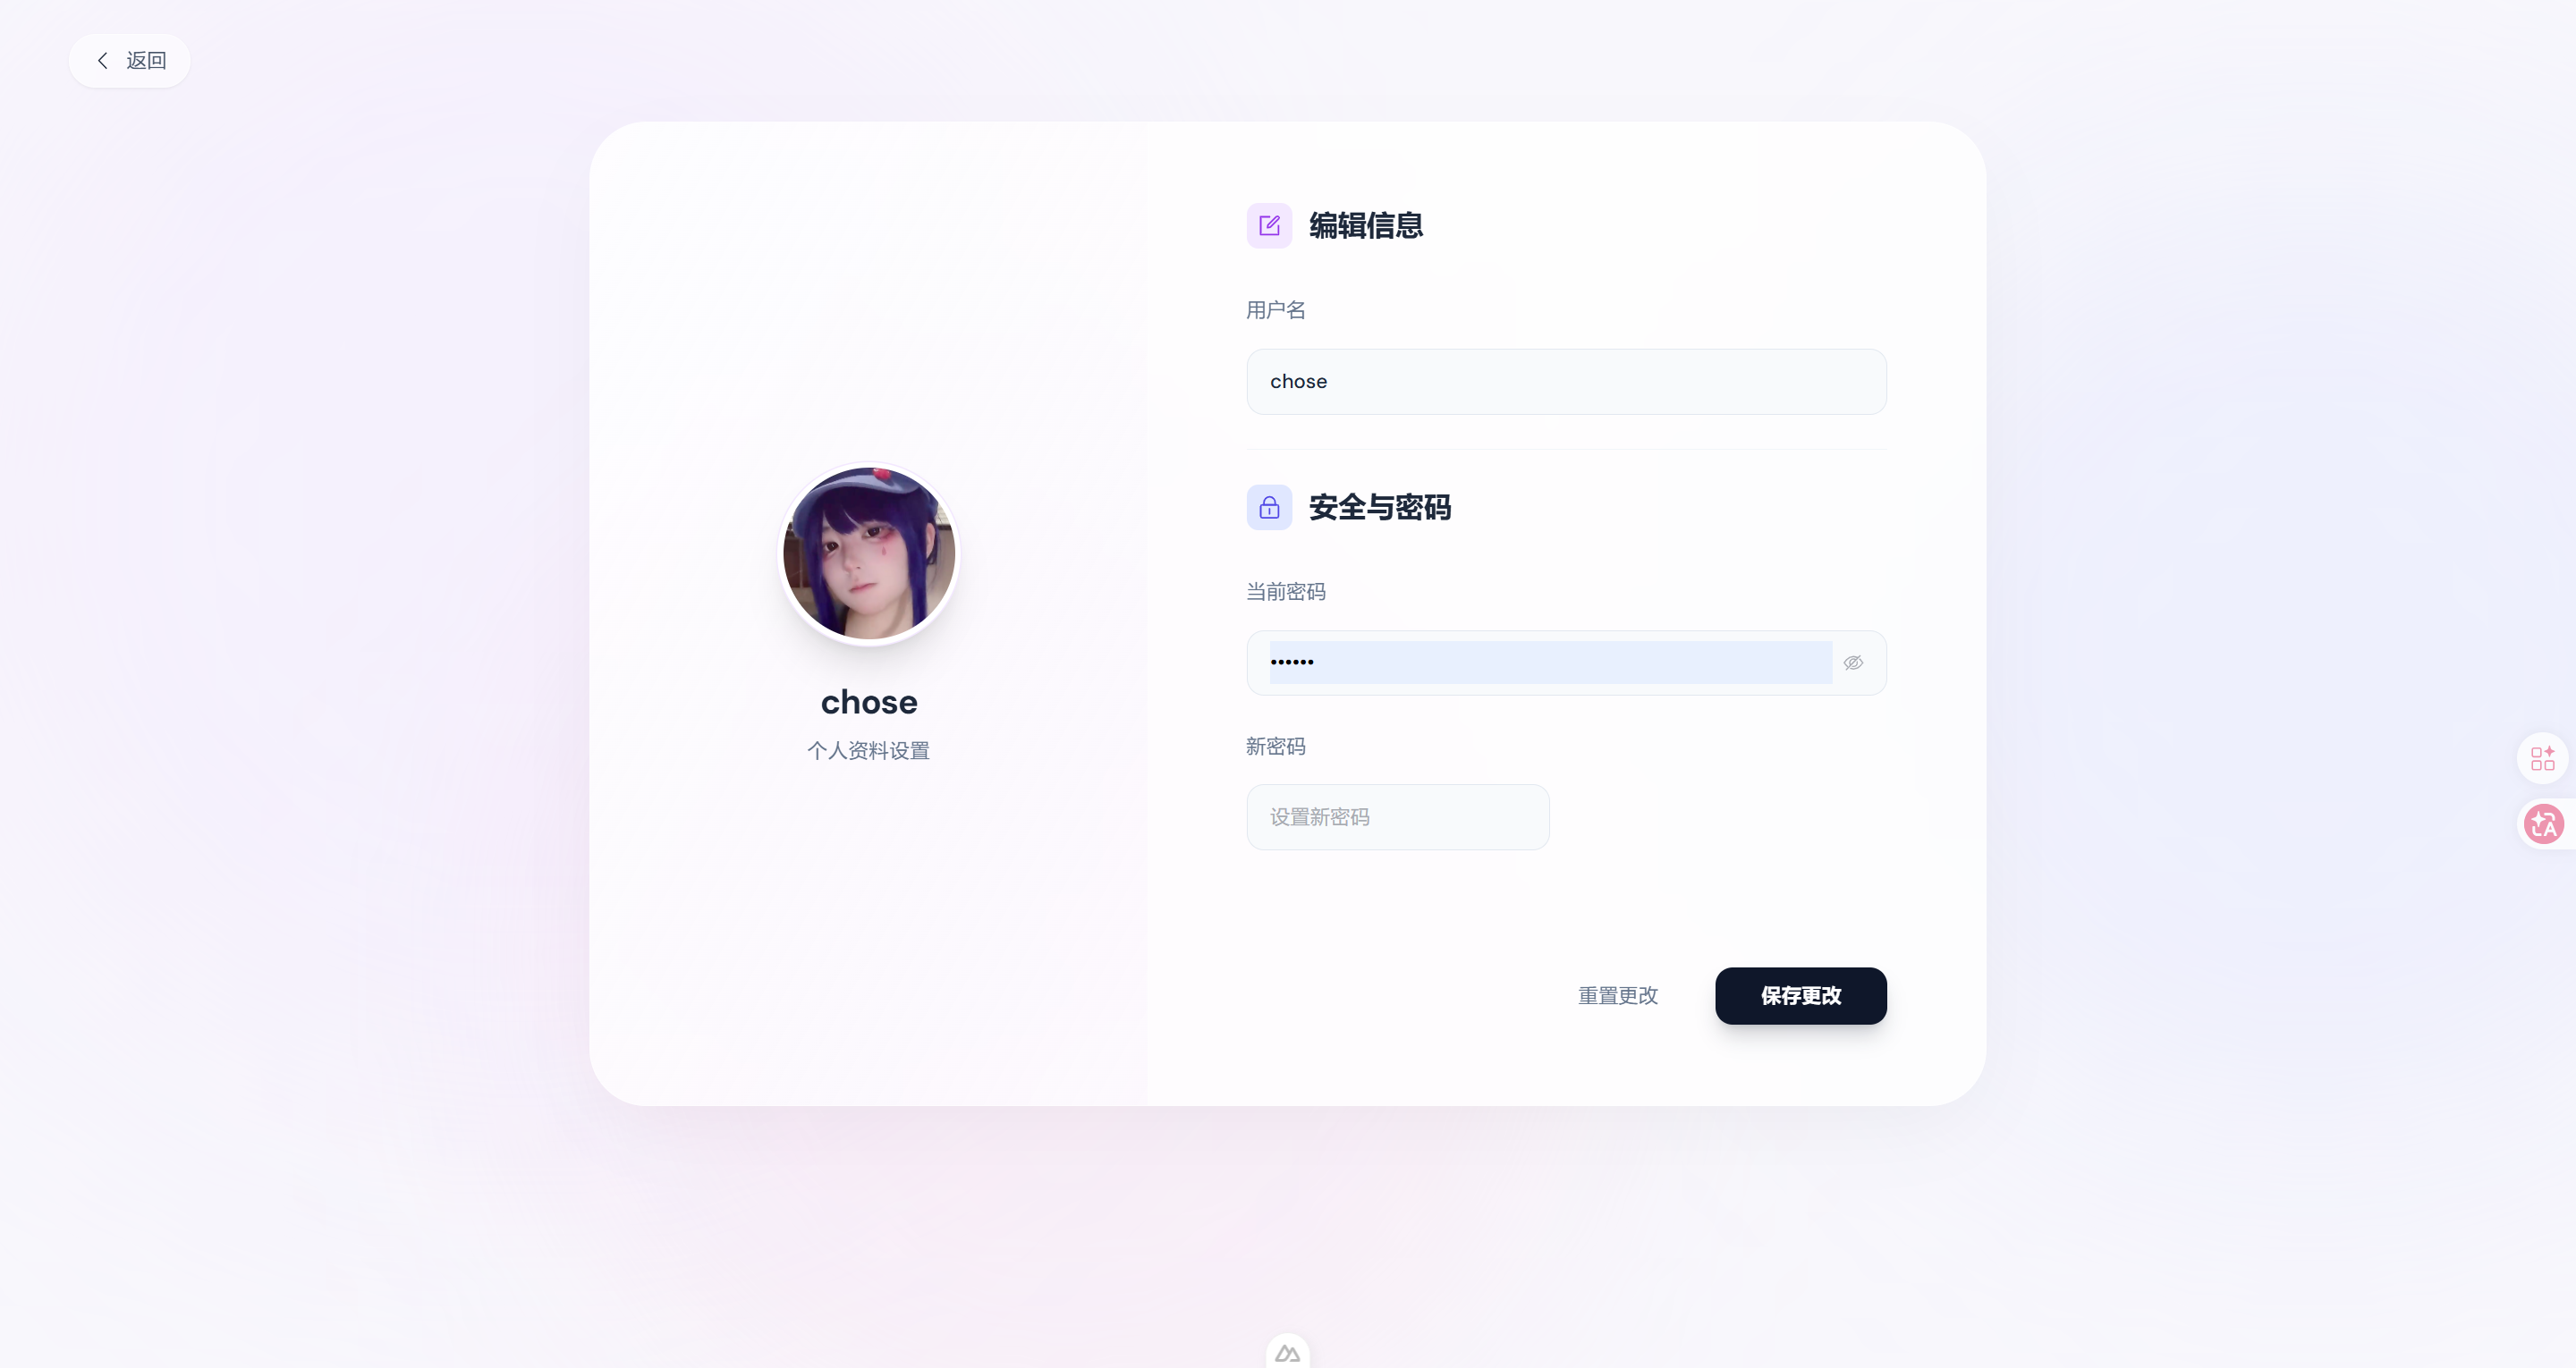
\includegraphics[width=0.85\textwidth]{test3}
	\caption{个人信息展示}
	\label{fig:test-profile}
\end{figure}

\begin{figure}[H]
	\centering
	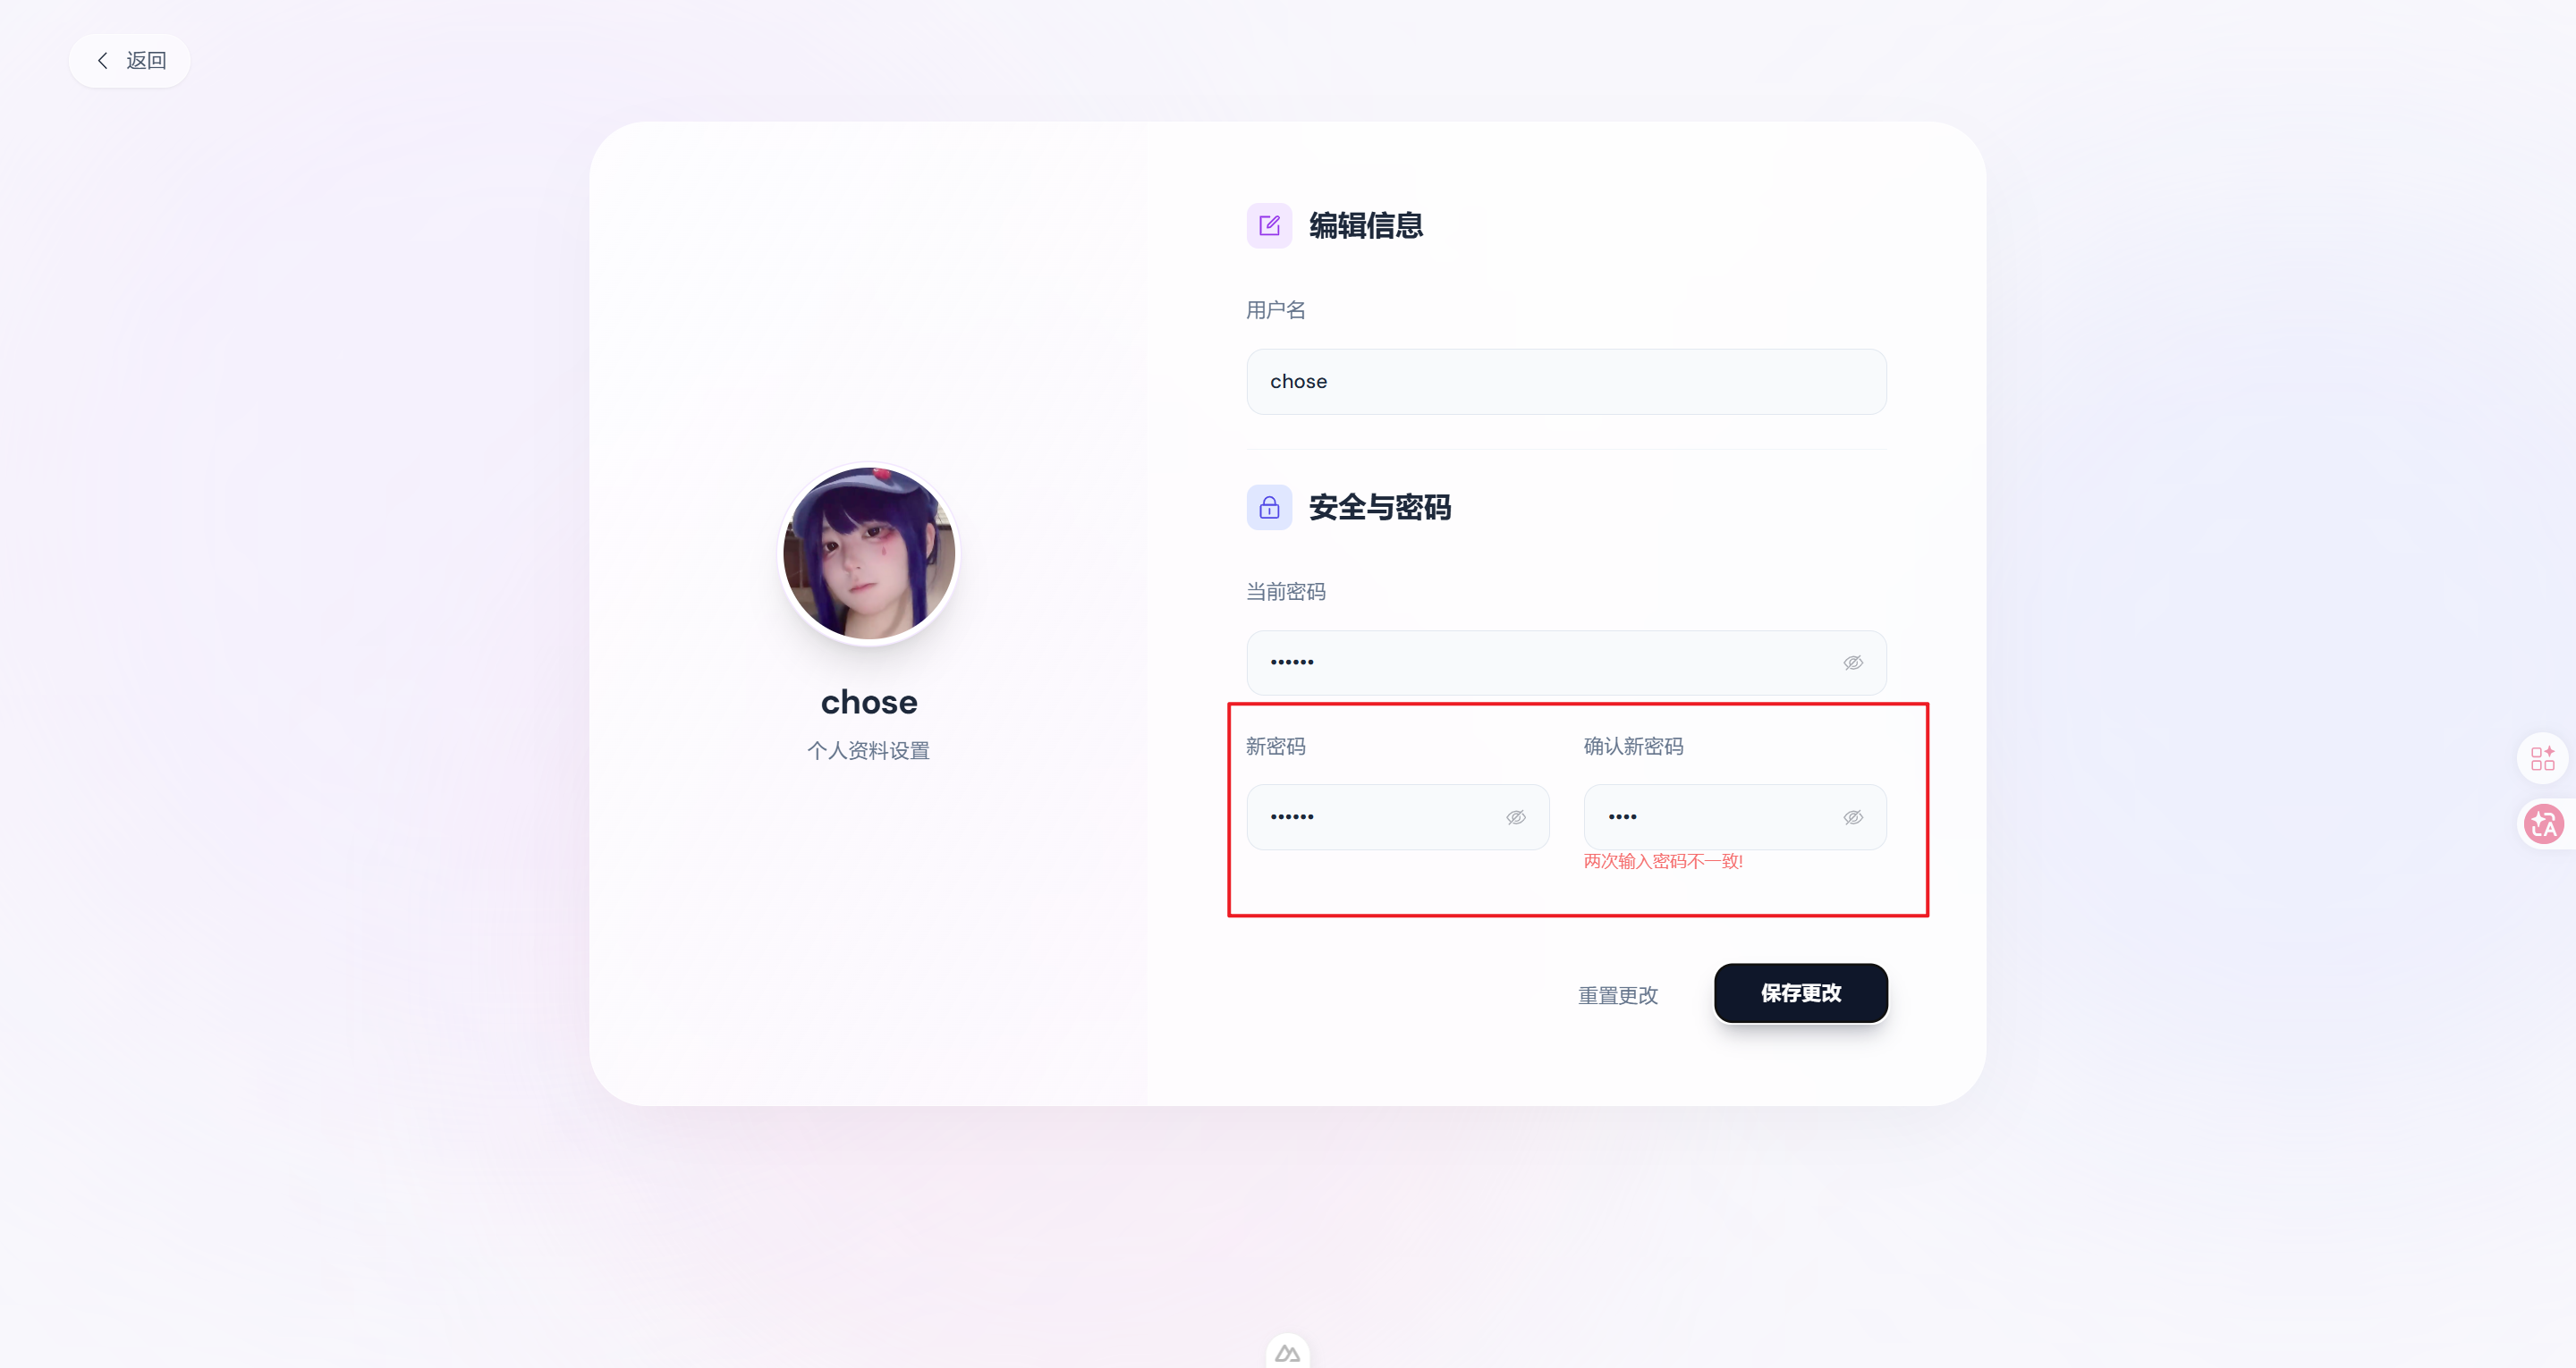
\includegraphics[width=0.85\textwidth]{test4}
	\caption{修改密码校验}
	\label{fig:test-password-check}
\end{figure}

\subsection{3D 服装定制模块测试}

3D 服装定制模块主要覆盖“选择款式—参数调整—3D 预览—保存”的完整链路，并验证渲染交互与数据保存的正确性。

\subsubsection{进入定制与资源加载}

测试用例如表~\ref{tab:testcase-customize-load}所示。

\begin{table}[H]
	\centering
	\caption{进入定制与资源加载测试用例}
	\label{tab:testcase-customize-load}
	\renewcommand{\arraystretch}{1.25}
	\setlength{\tabcolsep}{0.2ex}
	\begin{tabularx}{\textwidth}{@{}>{\raggedright\arraybackslash}p{0.12\textwidth} >{\raggedright\arraybackslash}p{0.22\textwidth} >{\raggedright\arraybackslash}X >{\raggedright\arraybackslash}X@{}}
		\toprule
		\textbf{\mbox{用例ID}} & \textbf{\mbox{前置条件}} & \textbf{\mbox{测试步骤}} & \textbf{\mbox{期望结果}} \\
		\midrule
		\mbox{003} & 已登录（若该模块需要登录）；网络稳定。 & 1. 从首页/功能入口进入 3D 定制页面；\newline 2. 观察模型、材质、纹理加载过程与加载提示。 & 1. 进入页面后可预览 3D 服装；\newline 2. 加载完成后模型显示完整，无明显缺面/贴图错误。 \\
		\bottomrule
	\end{tabularx}
\end{table}

测试结果与期望一致：3D 模型及材质纹理加载完成后显示完整，无明显缺面或贴图异常，加载状态提示清晰。如图~\ref{fig:test-model-square}所示。

\begin{figure}[H]
	\centering
	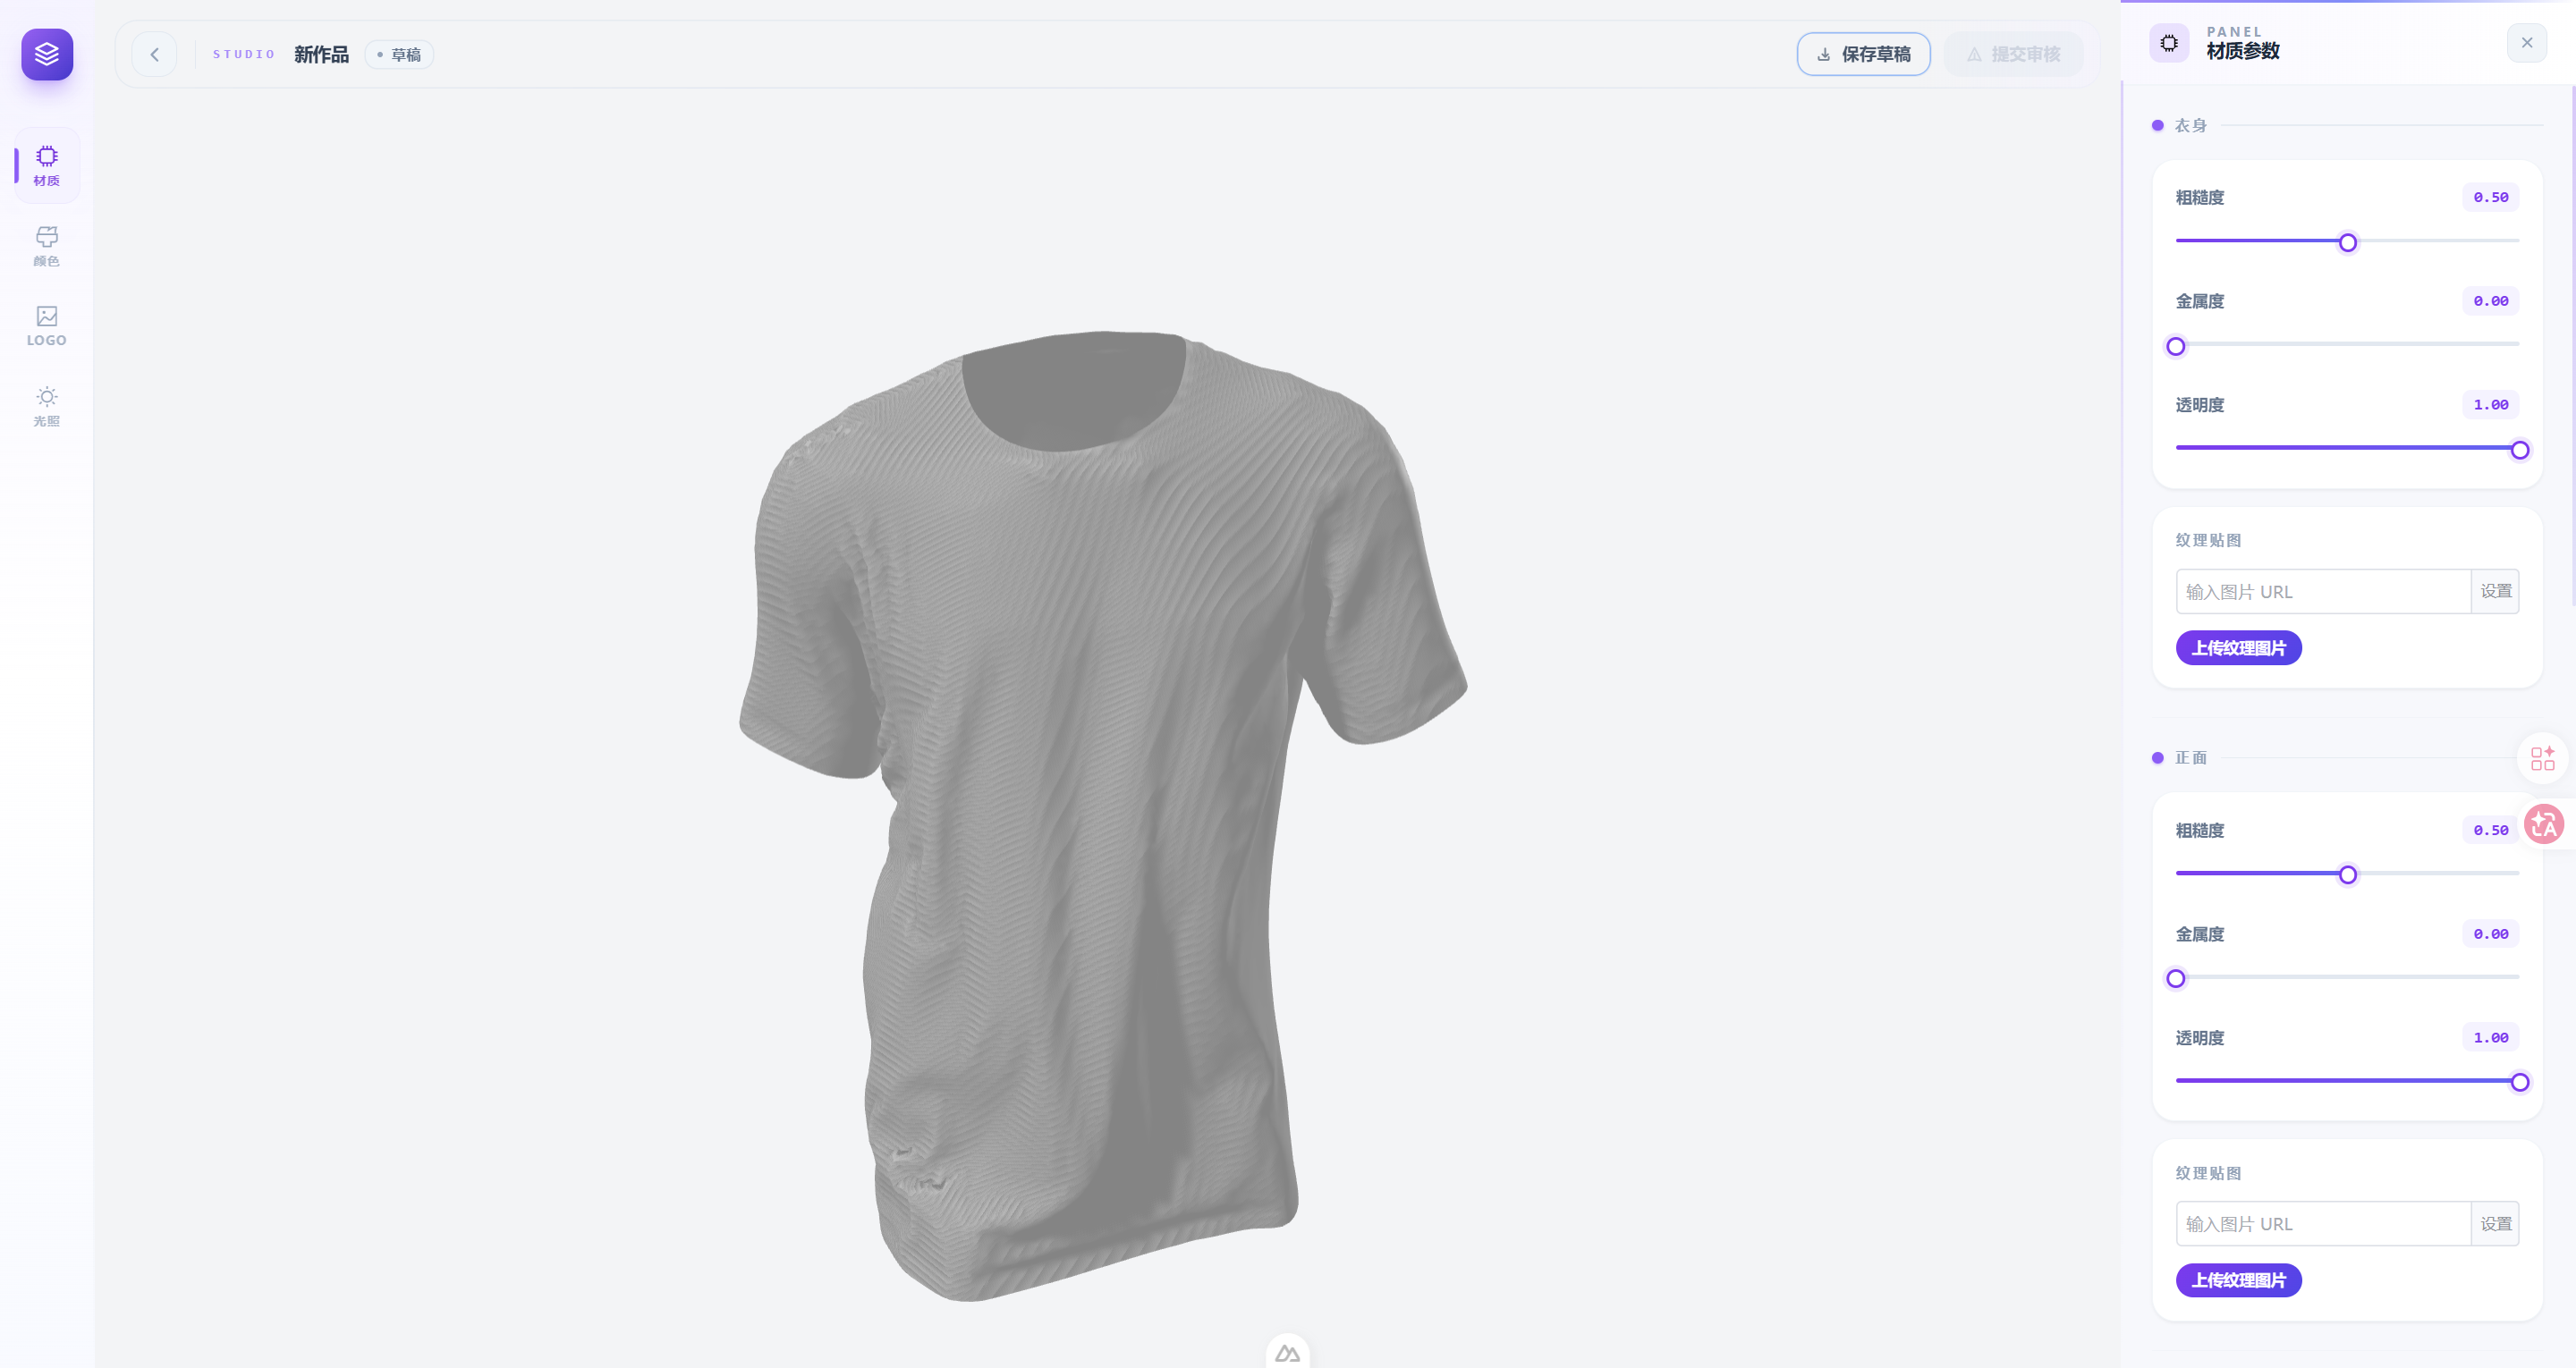
\includegraphics[width=0.85\textwidth]{test5}
	\caption{模型广场展示}
	\label{fig:test-model-square}
\end{figure}

\subsubsection{款式与属性配置}

测试用例如表~\ref{tab:testcase-style-config}所示。

\begin{table}[H]
	\centering
	\caption{款式与属性配置测试用例}
	\label{tab:testcase-style-config}
	\renewcommand{\arraystretch}{1.25}
	\setlength{\tabcolsep}{0.2ex}
	\begin{tabularx}{\textwidth}{@{}>{\raggedright\arraybackslash}p{0.12\textwidth} >{\raggedright\arraybackslash}p{0.22\textwidth} >{\raggedright\arraybackslash}X >{\raggedright\arraybackslash}X@{}}
		\toprule
		\textbf{\mbox{用例ID}} & \textbf{\mbox{前置条件}} & \textbf{\mbox{测试步骤}} & \textbf{\mbox{期望结果}} \\
		\midrule
		\mbox{004} & 3D 模型已加载完成。 & 1. 选择不同服装款式；\newline 2. 调整颜色、面料/材质、图案等属性，观察 3D 视图实时变化。 & 1. 属性变更即时反映到模型，显示效果与选择项一致；\newline 2. 参数边界有合理限制（最小/最大值、步进、非法输入拦截）。 \\
		\bottomrule
	\end{tabularx}
\end{table}

测试结果与期望一致：款式切换正确，颜色/材质/图案等属性修改可实时反映到 3D 模型且与选择项一致，参数边界限制合理。结果如图~\ref{fig:test-model-select}和图~\ref{fig:test-model-edit}所示。

\begin{figure}[H]
	\centering
	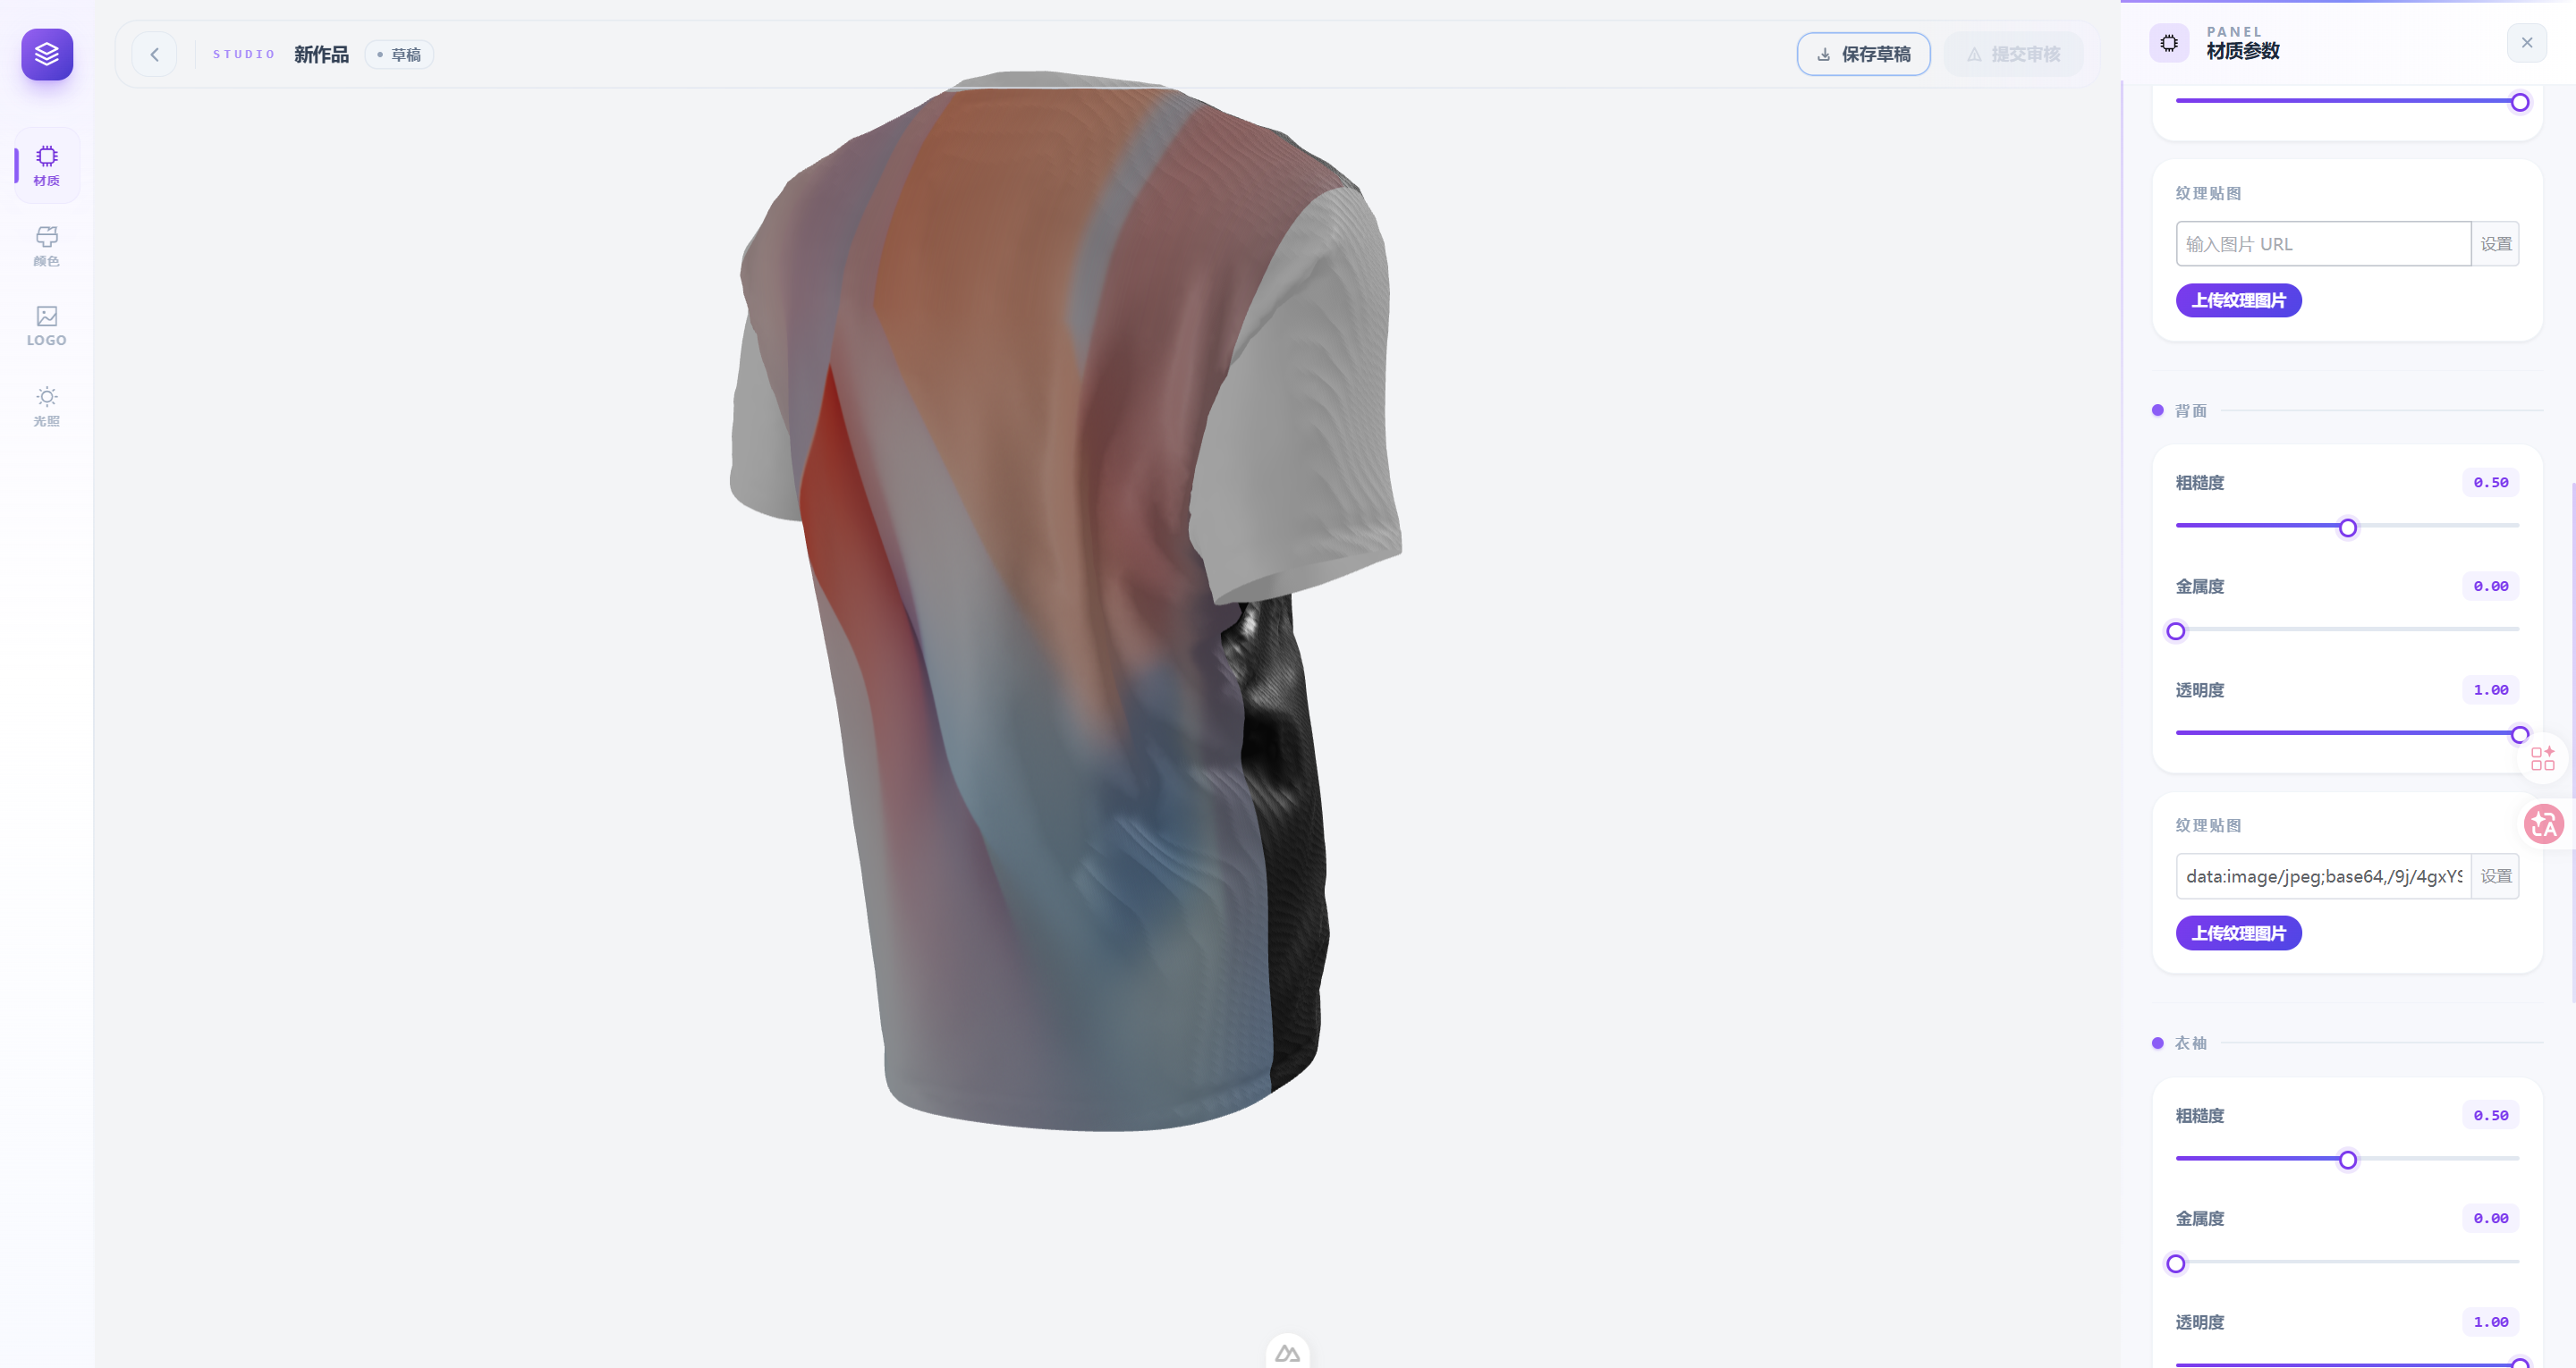
\includegraphics[width=0.85\textwidth]{test6}
	\caption{模型选择展示}
	\label{fig:test-model-select}
\end{figure}

\begin{figure}[H]
	\centering
	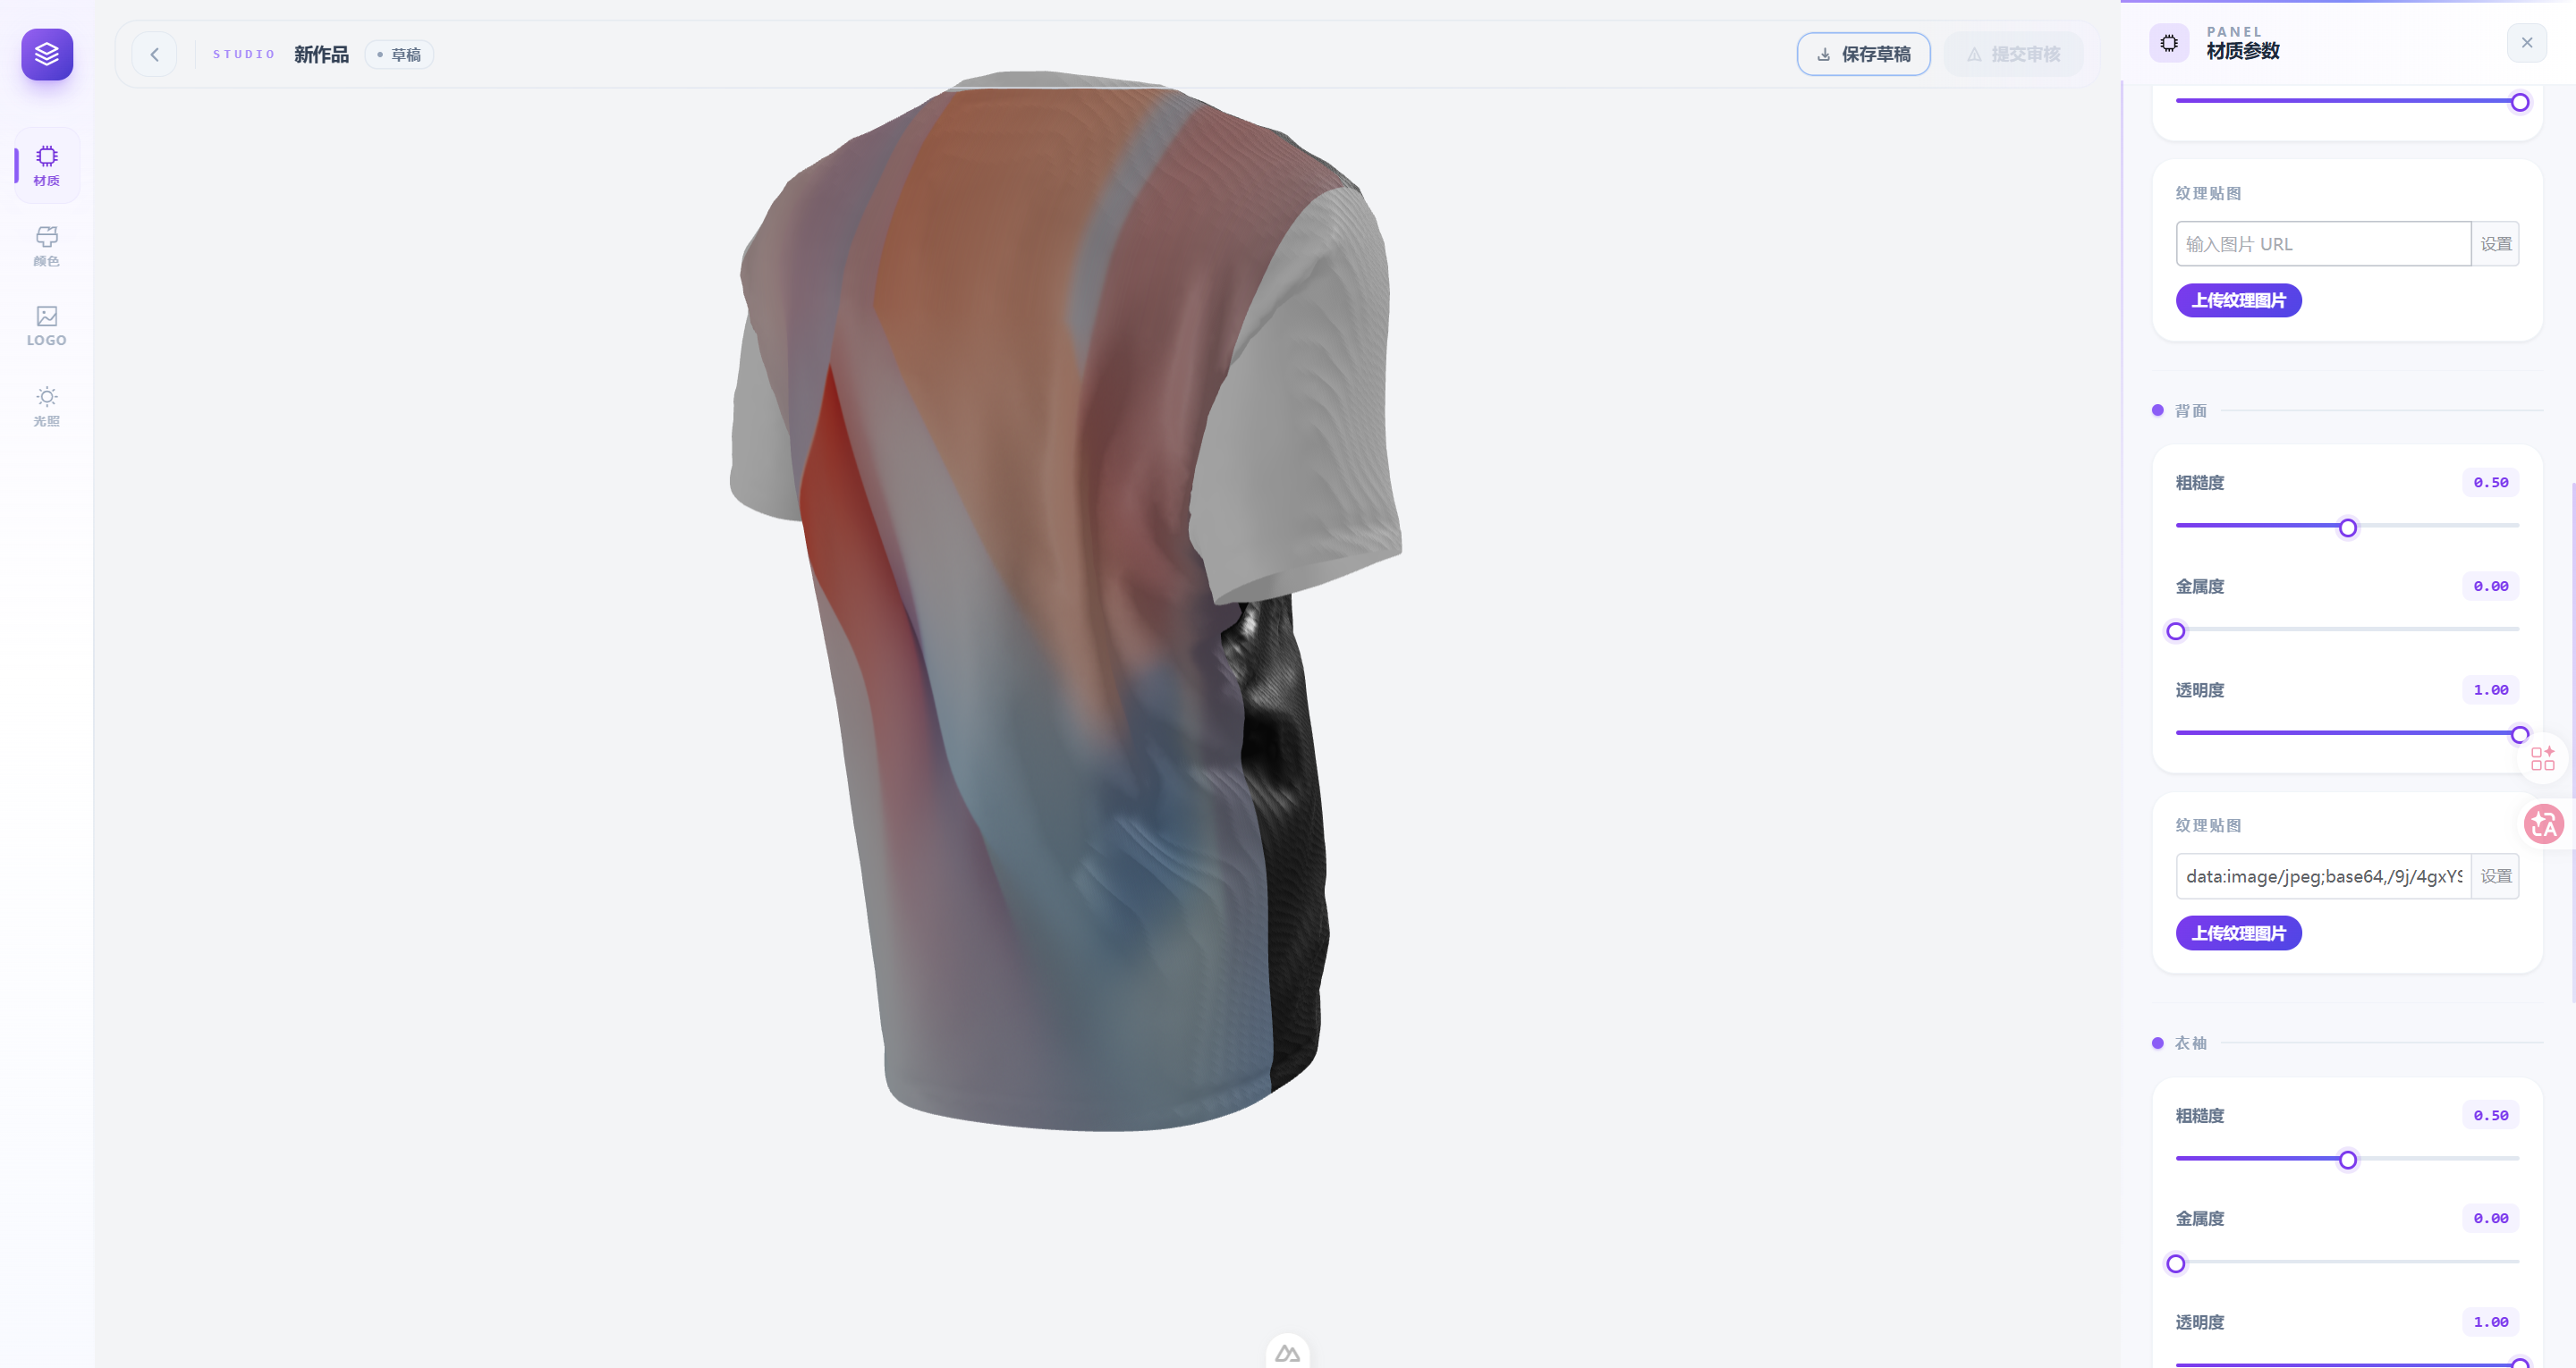
\includegraphics[width=0.85\textwidth]{test7}
	\caption{模型编辑成功展示}
	\label{fig:test-model-edit}
\end{figure}

\subsubsection{3D 交互与预览验证}

测试用例如表~\ref{tab:testcase-3d-interaction}所示。

\begin{table}[H]
	\centering
	\caption{3D 交互与预览验证测试用例}
	\label{tab:testcase-3d-interaction}
	\renewcommand{\arraystretch}{1.25}
	\setlength{\tabcolsep}{0.2ex}
	\begin{tabularx}{\textwidth}{@{}>{\raggedright\arraybackslash}p{0.12\textwidth} >{\raggedright\arraybackslash}p{0.22\textwidth} >{\raggedright\arraybackslash}X >{\raggedright\arraybackslash}X@{}}
		\toprule
		\textbf{\mbox{用例ID}} & \textbf{\mbox{前置条件}} & \textbf{\mbox{测试步骤}} & \textbf{\mbox{期望结果}} \\
		\midrule
		\mbox{005} & 模型可交互。 & 1. 测试旋转、缩放等交互；\newline 2. 切换不同视角，检查渲染是否稳定、帧率是否可接受；\newline 3. 在不同分辨率下查看布局是否错位。 & 1. 交互响应顺畅；重置视角可恢复默认状态；\newline 2. 关键组件（按钮/面板）不遮挡核心操作，布局自适应正常。 \\
		\bottomrule
	\end{tabularx}
\end{table}

测试结果与期望一致：旋转、缩放等交互响应顺畅，重置视角可恢复默认状态，页面布局自适应正常。如图~\ref{fig:test-model-interaction}所示。

\begin{figure}[H]
	\centering
	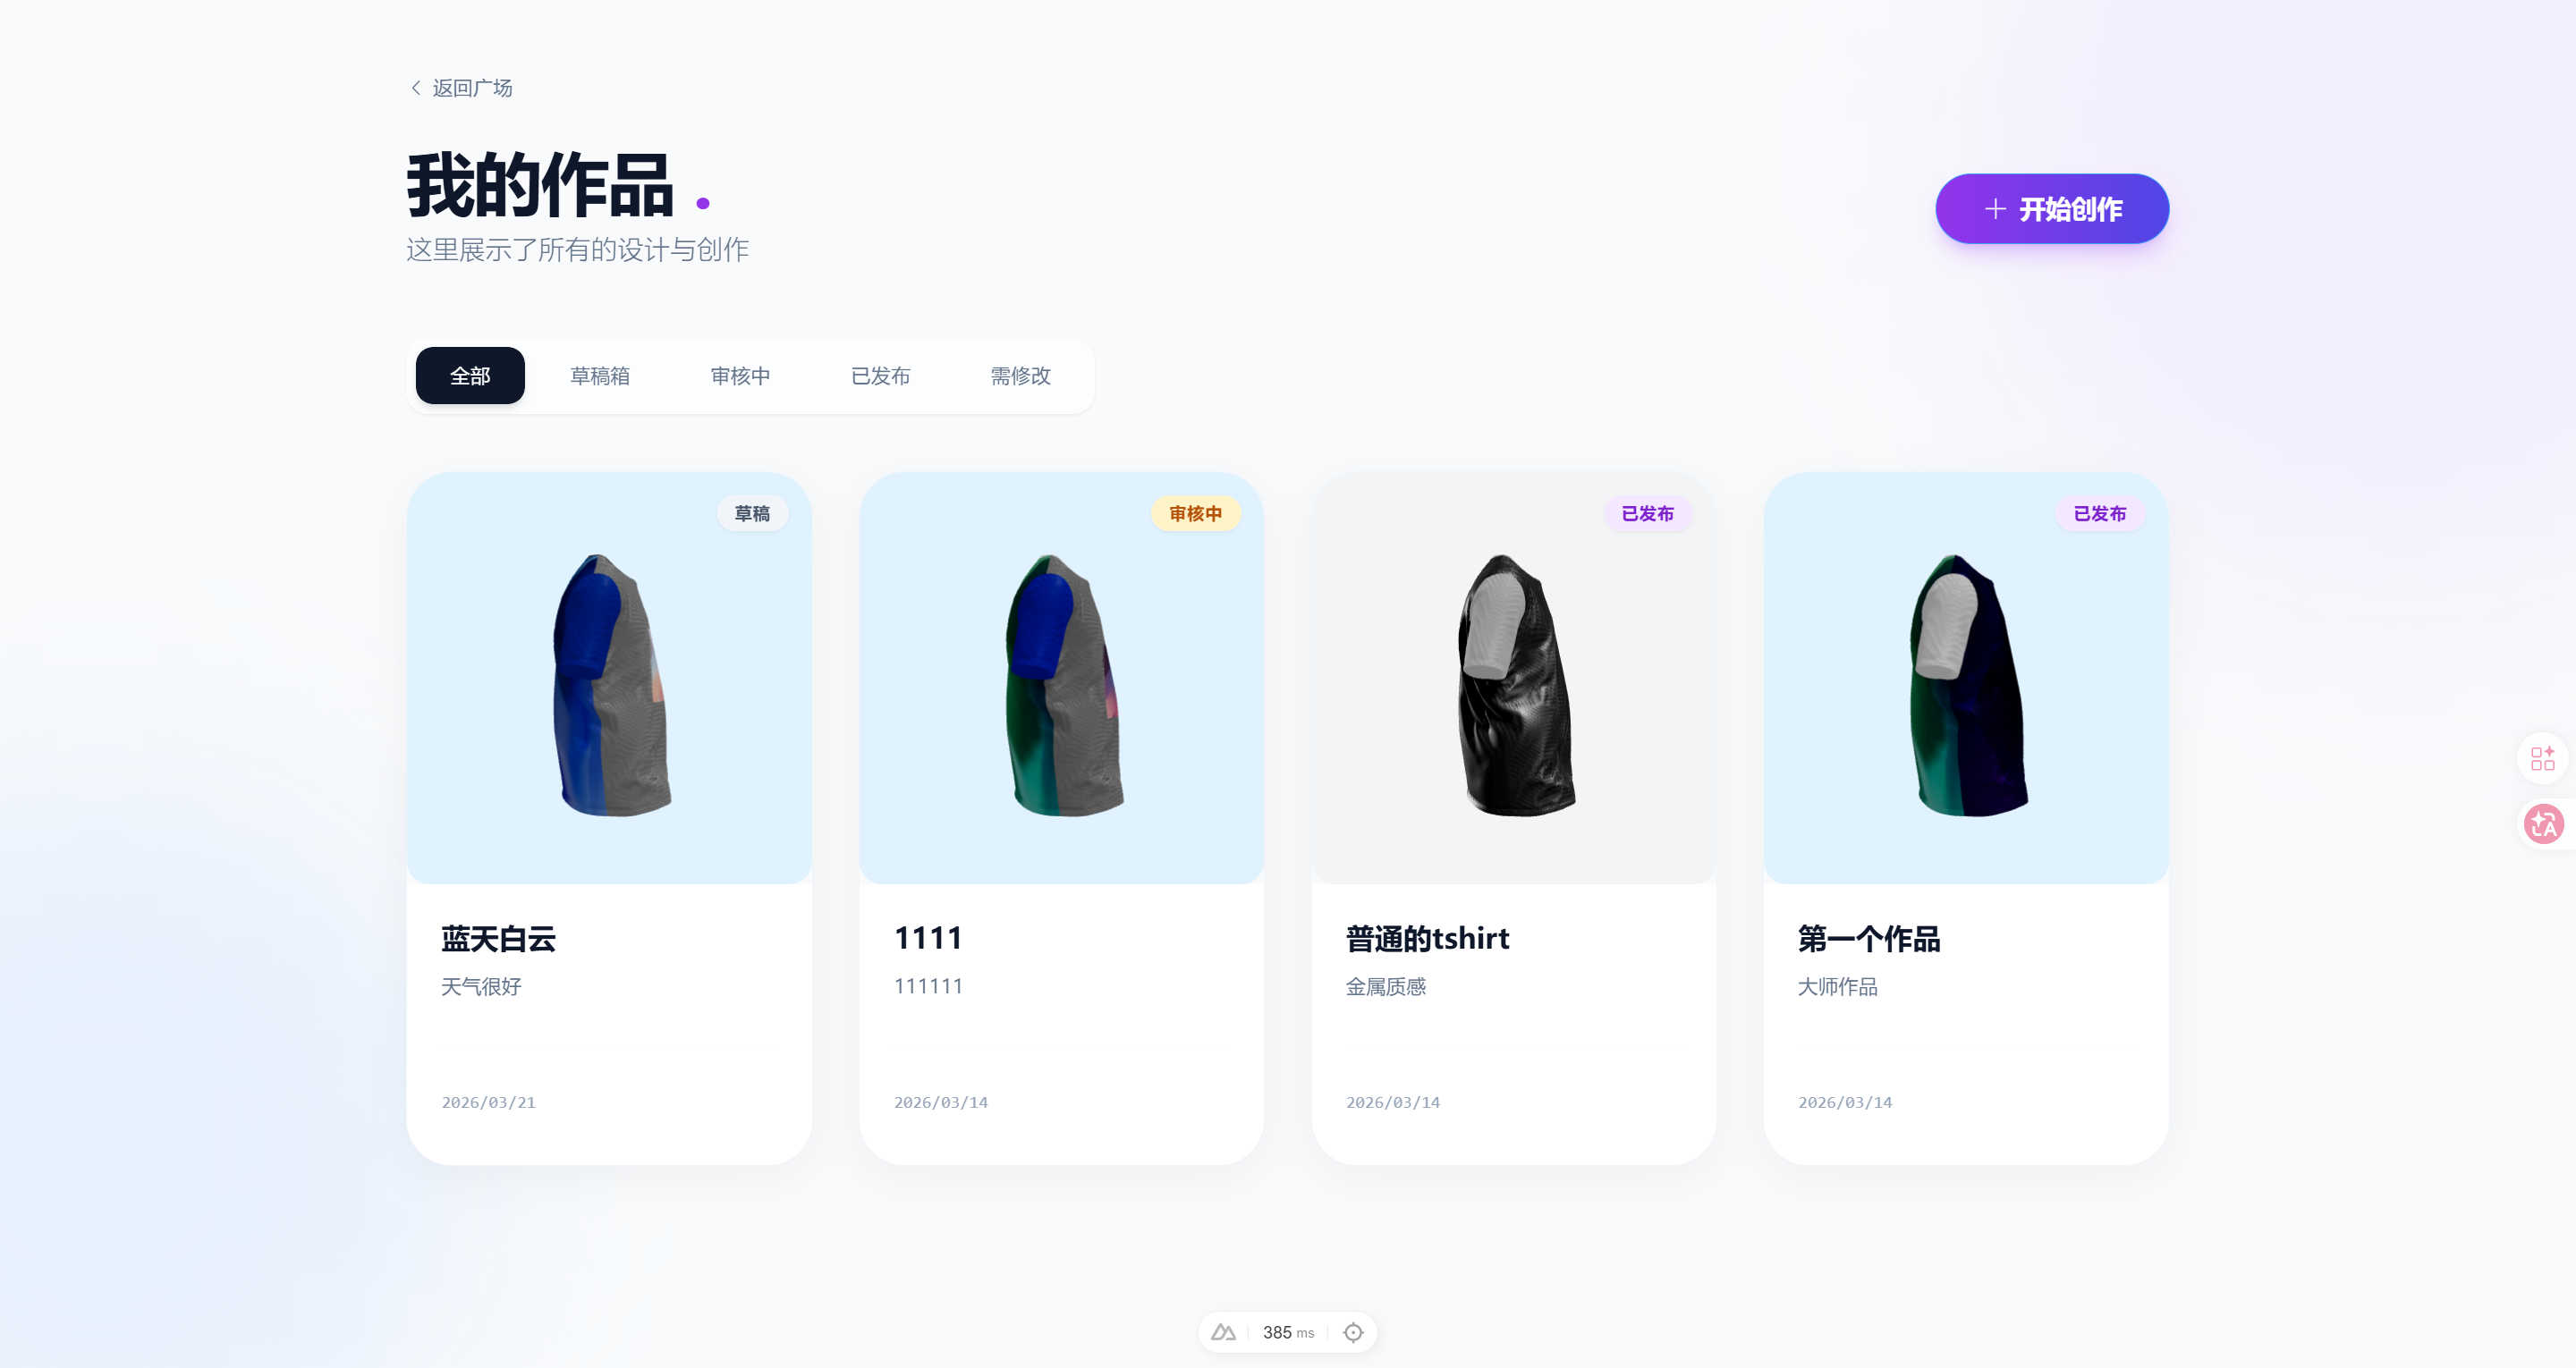
\includegraphics[width=0.85\textwidth]{test8}
	\caption{模型交互展示}
	\label{fig:test-model-interaction}
\end{figure}

\subsubsection{方案保存与后续流转}

测试用例如表~\ref{tab:testcase-plan-save}所示。

\begin{table}[H]
	\centering
	\caption{方案保存与后续流转测试用例}
	\label{tab:testcase-plan-save}
	\renewcommand{\arraystretch}{1.25}
	\setlength{\tabcolsep}{0.2ex}
	\begin{tabularx}{\textwidth}{@{}>{\raggedright\arraybackslash}p{0.12\textwidth} >{\raggedright\arraybackslash}p{0.22\textwidth} >{\raggedright\arraybackslash}X >{\raggedright\arraybackslash}X@{}}
		\toprule
		\textbf{\mbox{用例ID}} & \textbf{\mbox{前置条件}} & \textbf{\mbox{测试步骤}} & \textbf{\mbox{期望结果}} \\
		\midrule
		\mbox{006} & 已完成一组定制参数。 & 1. 点击保存，存储草稿并提交审核；\newline 2. 进入“我的作品”查看保存记录是否存在，参数是否一致；\newline 3. 删除/编辑保存记录，检查更新是否正确。 & 1. 保存成功提示明确；保存后数据可在列表中查询并正确回显；\newline 2. 编辑/删除操作生效且不影响其他记录。 \\
		\bottomrule
	\end{tabularx}
\end{table}

测试结果与期望一致：方案保存成功提示明确，保存记录可在“我的作品”列表查询并正确回显，编辑/删除后数据一致。如图~\ref{fig:test-work-status-3d}所示。

\begin{figure}[H]
	\centering
	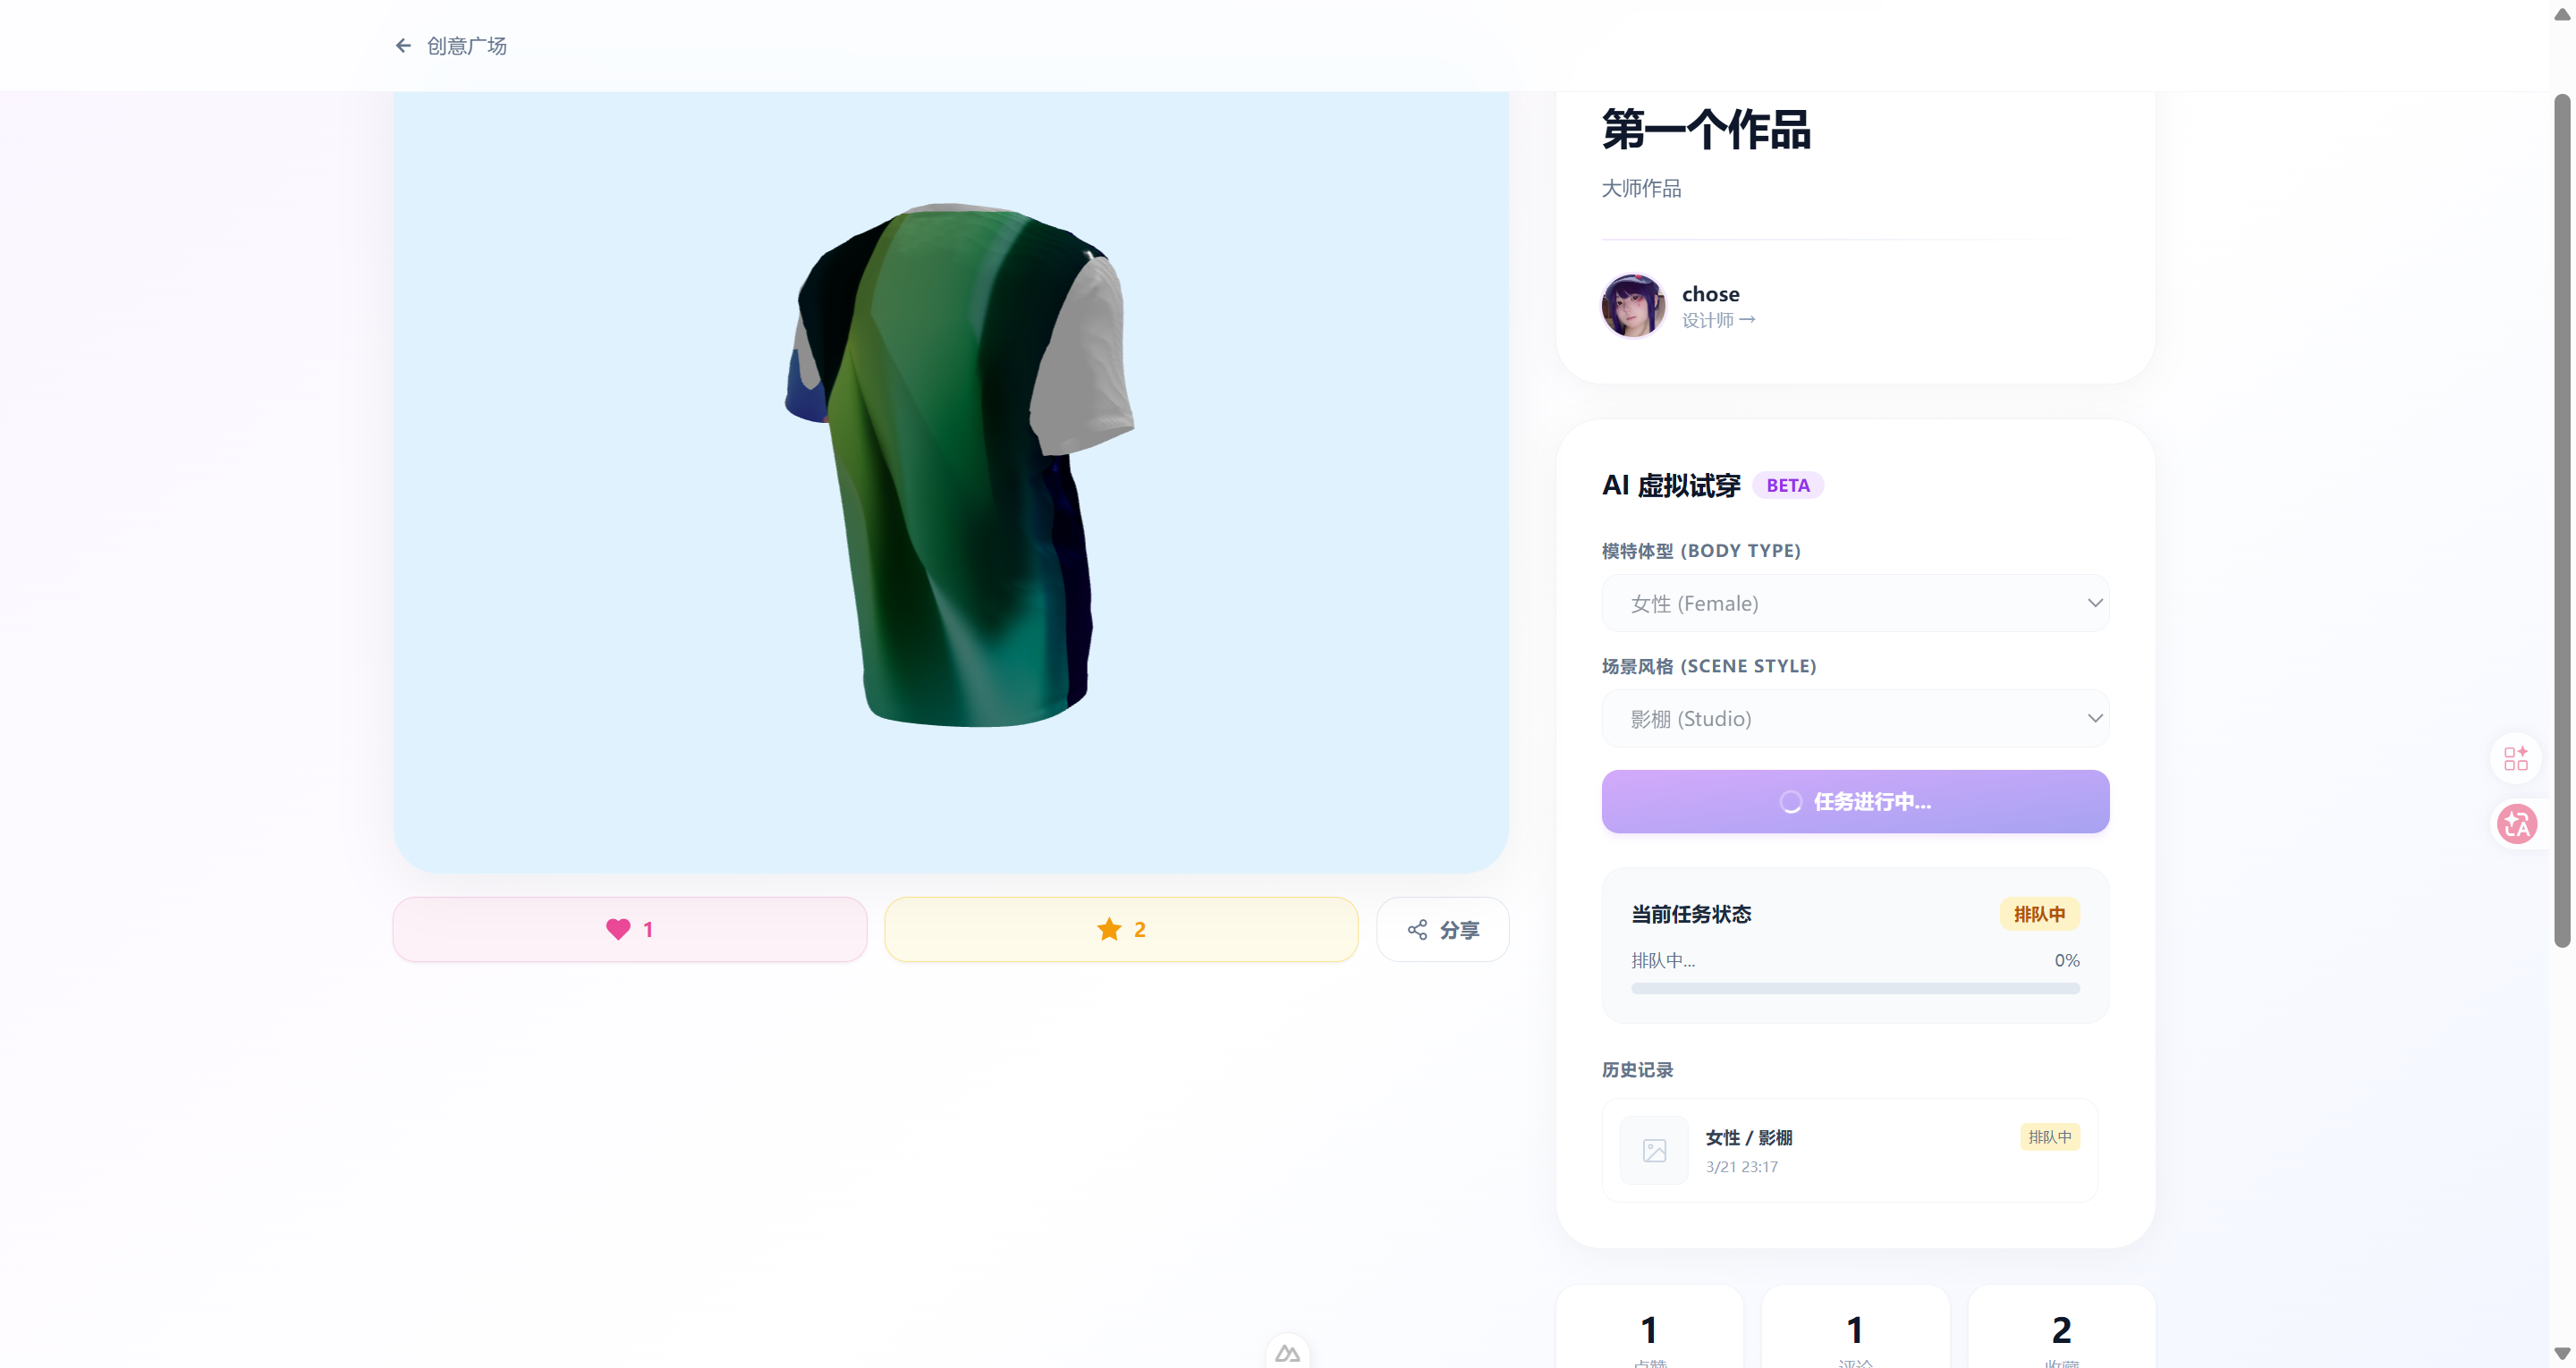
\includegraphics[width=0.85\textwidth]{test9}
	\caption{作品状态展示}
	\label{fig:test-work-status-3d}
\end{figure}

\subsection{AI 虚拟试穿模块测试}

AI 虚拟试穿模块主要覆盖“输入准备—提交生成—结果展示—历史管理”的流程，并重点验证任务状态、异常提示与结果可用性。

\subsubsection{试穿任务创建}

测试用例如表~\ref{tab:testcase-tryon-create}所示。

\begin{table}[H]
	\centering
	\caption{试穿任务创建测试用例}
	\label{tab:testcase-tryon-create}
	\renewcommand{\arraystretch}{1.25}
	\setlength{\tabcolsep}{0.2ex}
	\begin{tabularx}{\textwidth}{@{}>{\raggedright\arraybackslash}p{0.12\textwidth} >{\raggedright\arraybackslash}p{0.22\textwidth} >{\raggedright\arraybackslash}X >{\raggedright\arraybackslash}X@{}}
		\toprule
		\textbf{\mbox{用例ID}} & \textbf{\mbox{前置条件}} & \textbf{\mbox{测试步骤}} & \textbf{\mbox{期望结果}} \\
		\midrule
		\mbox{007} & 已登录；具备可选服装。 & 1. 进入作品详情页面，选择模特性别及场景；\newline 2. 点击“开始试穿/生成”提交任务。 & 1. 提交后显示任务状态（排队），并防止重复提交造成多任务堆积（如按钮置灰）。 \\
		\bottomrule
	\end{tabularx}
\end{table}

测试结果与期望一致：试穿任务提交后状态展示正常（排队/生成中），并具备防重复提交机制（按钮置灰/提示）。如图~\ref{fig:test-ai-create}所示。

\begin{figure}[H]
	\centering
	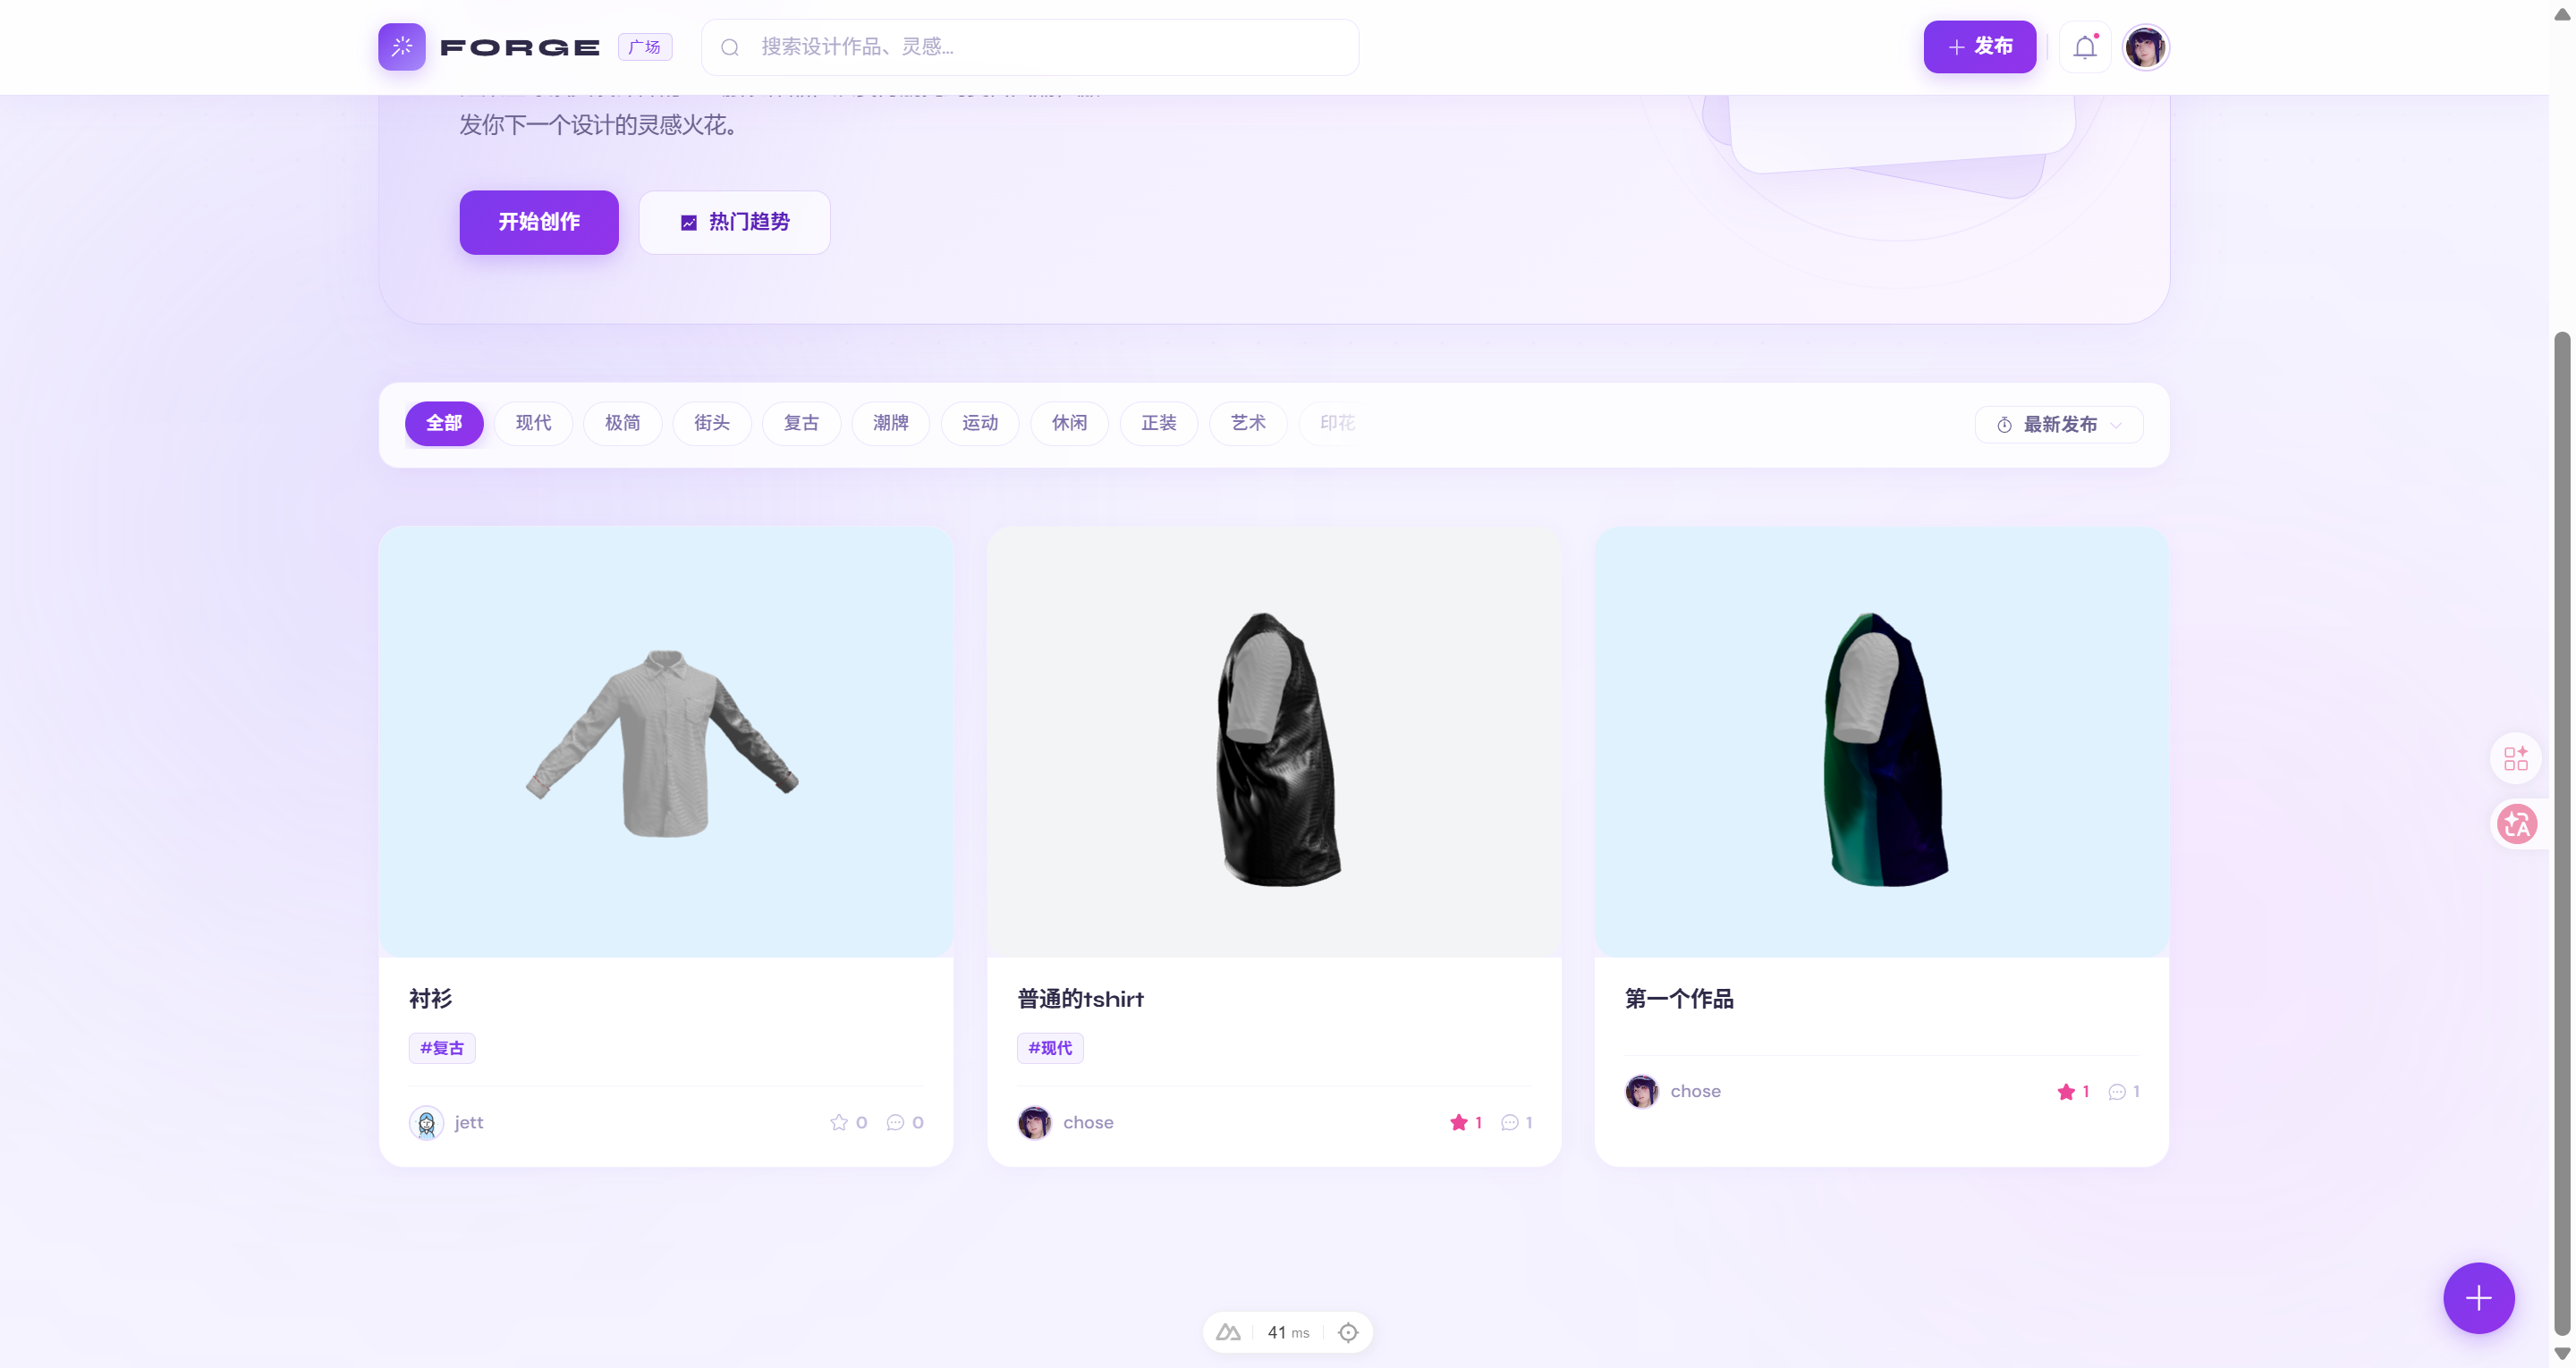
\includegraphics[width=0.85\textwidth]{test10}
	\caption{AI 试穿创建任务展示}
	\label{fig:test-ai-create}
\end{figure}

\subsubsection{生成过程与结果展示}

测试用例如表~\ref{tab:testcase-tryon-result}所示。

\begin{table}[H]
	\centering
	\caption{生成过程与结果展示测试用例}
	\label{tab:testcase-tryon-result}
	\renewcommand{\arraystretch}{1.25}
	\setlength{\tabcolsep}{0.2ex}
	\begin{tabularx}{\textwidth}{@{}>{\raggedright\arraybackslash}p{0.12\textwidth} >{\raggedright\arraybackslash}p{0.22\textwidth} >{\raggedright\arraybackslash}X >{\raggedright\arraybackslash}X@{}}
		\toprule
		\textbf{\mbox{用例ID}} & \textbf{\mbox{前置条件}} & \textbf{\mbox{测试步骤}} & \textbf{\mbox{期望结果}} \\
		\midrule
		\mbox{008} & 任务已提交。 & 1. 观察生成进度提示与历史记录展示；\newline 2. 生成完成后查看试穿图；\newline 3. 测试下载/再次生成等操作。 & 1. 生成完成后自动刷新或提供可操作入口，不出现“生成完成但页面不更新”的问题；\newline 2. 结果可正常预览与下载；失败时返回可理解的错误原因与建议。 \\
		\bottomrule
	\end{tabularx}
\end{table}

测试结果与期望一致：生成完成后试穿结果可正常预览与下载（或保存），并提供明确入口；生成失败时错误提示清晰可理解。如图~\ref{fig:test-ai-result}所示。

\begin{figure}[H]
	\centering
	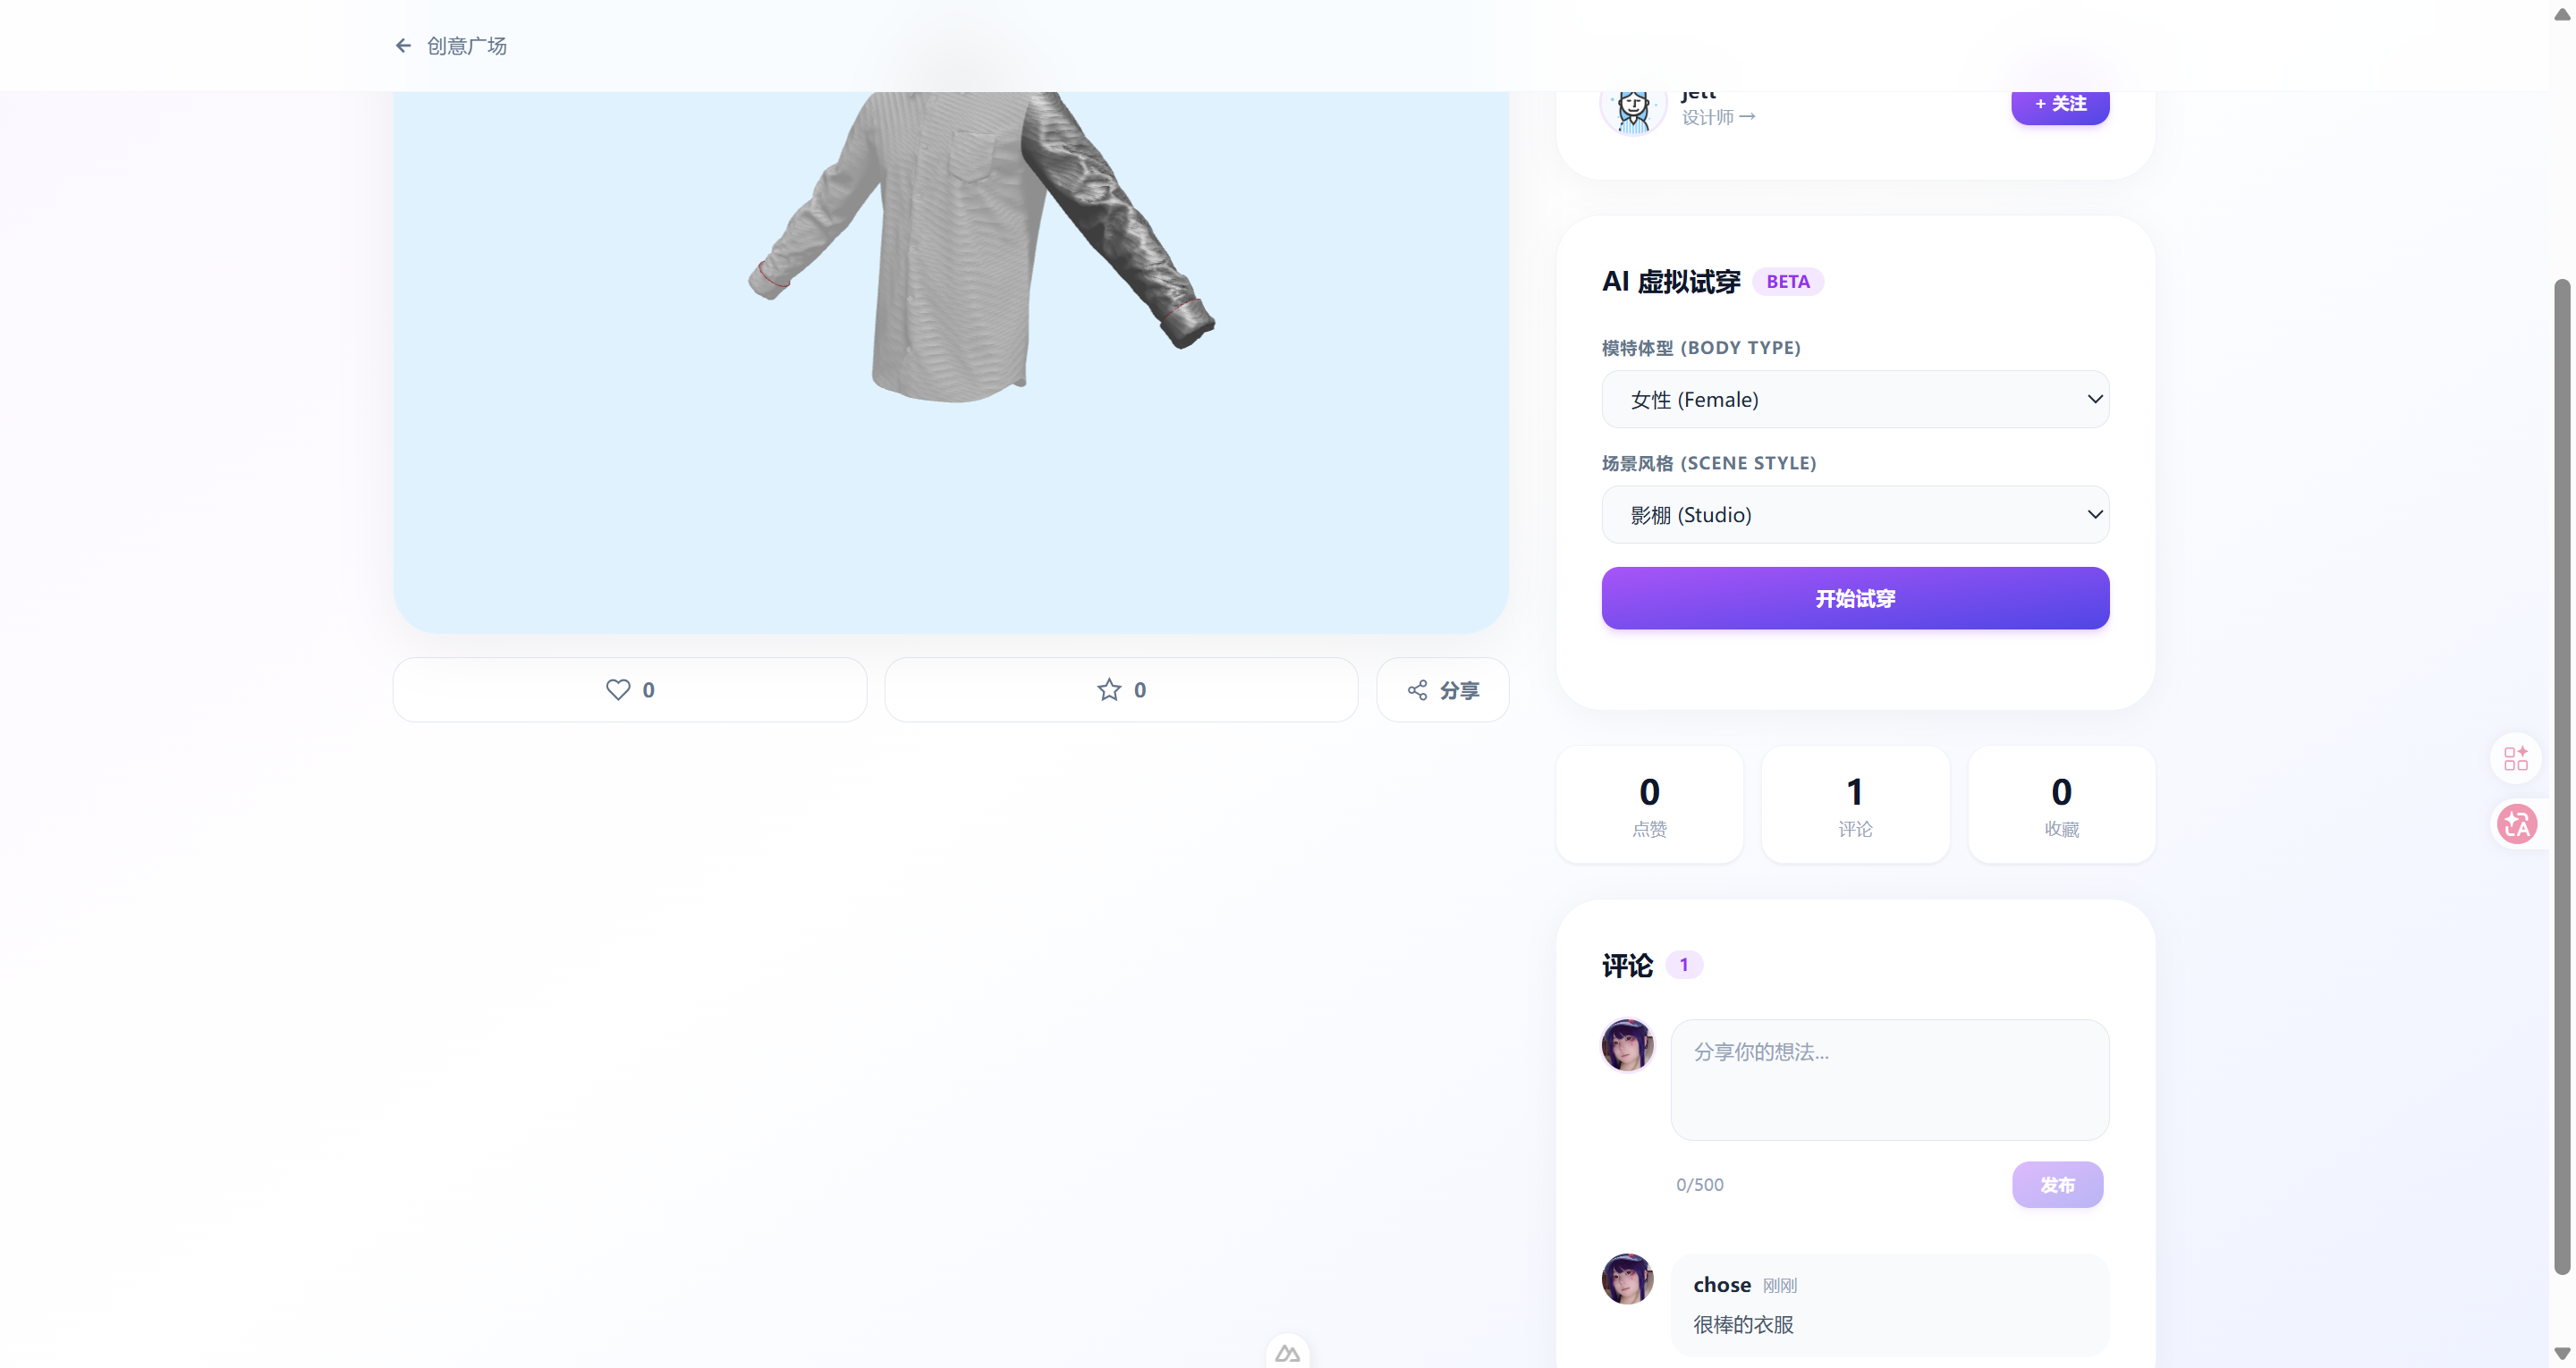
\includegraphics[width=0.85\textwidth]{test11}
	\caption{AI 试穿生成结果}
	\label{fig:test-ai-result}
\end{figure}

\subsection{创意广场模块测试}

创意广场模块主要覆盖内容浏览、搜索筛选、互动行为等功能，验证信息流展示与交互一致性。

\subsubsection{内容浏览与详情查看}

测试用例如表~\ref{tab:testcase-square-browse}所示。

\begin{table}[H]
	\centering
	\caption{内容浏览与详情查看测试用例}
	\label{tab:testcase-square-browse}
	\renewcommand{\arraystretch}{1.25}
	\setlength{\tabcolsep}{0.2ex}
	\begin{tabularx}{\textwidth}{@{}>{\raggedright\arraybackslash}p{0.12\textwidth} >{\raggedright\arraybackslash}p{0.22\textwidth} >{\raggedright\arraybackslash}X >{\raggedright\arraybackslash}X@{}}
		\toprule
		\textbf{\mbox{用例ID}} & \textbf{\mbox{前置条件}} & \textbf{\mbox{测试步骤}} & \textbf{\mbox{期望结果}} \\
		\midrule
		\mbox{009} & 已登录。 & 1. 进入创意广场，浏览推荐/最新等列表；\newline 2. 分页加载，检查加载提示与重复数据问题；\newline 3. 进入任意作品详情，查看图片/3D 展示（如有）、作者信息、标签等。 & 1. 列表加载顺序与规则正确；详情信息与列表项一致；\newline 2. 图片/资源加载失败有占位与重试，不影响主流程。 \\
		\bottomrule
	\end{tabularx}
\end{table}

测试结果与期望一致：创意广场列表加载顺序与展示规则正确，作品详情信息与列表项一致；资源加载异常时具备占位与重试机制，不影响主流程。如图~\ref{fig:test-creative-square}所示。

\begin{figure}[H]
	\centering
	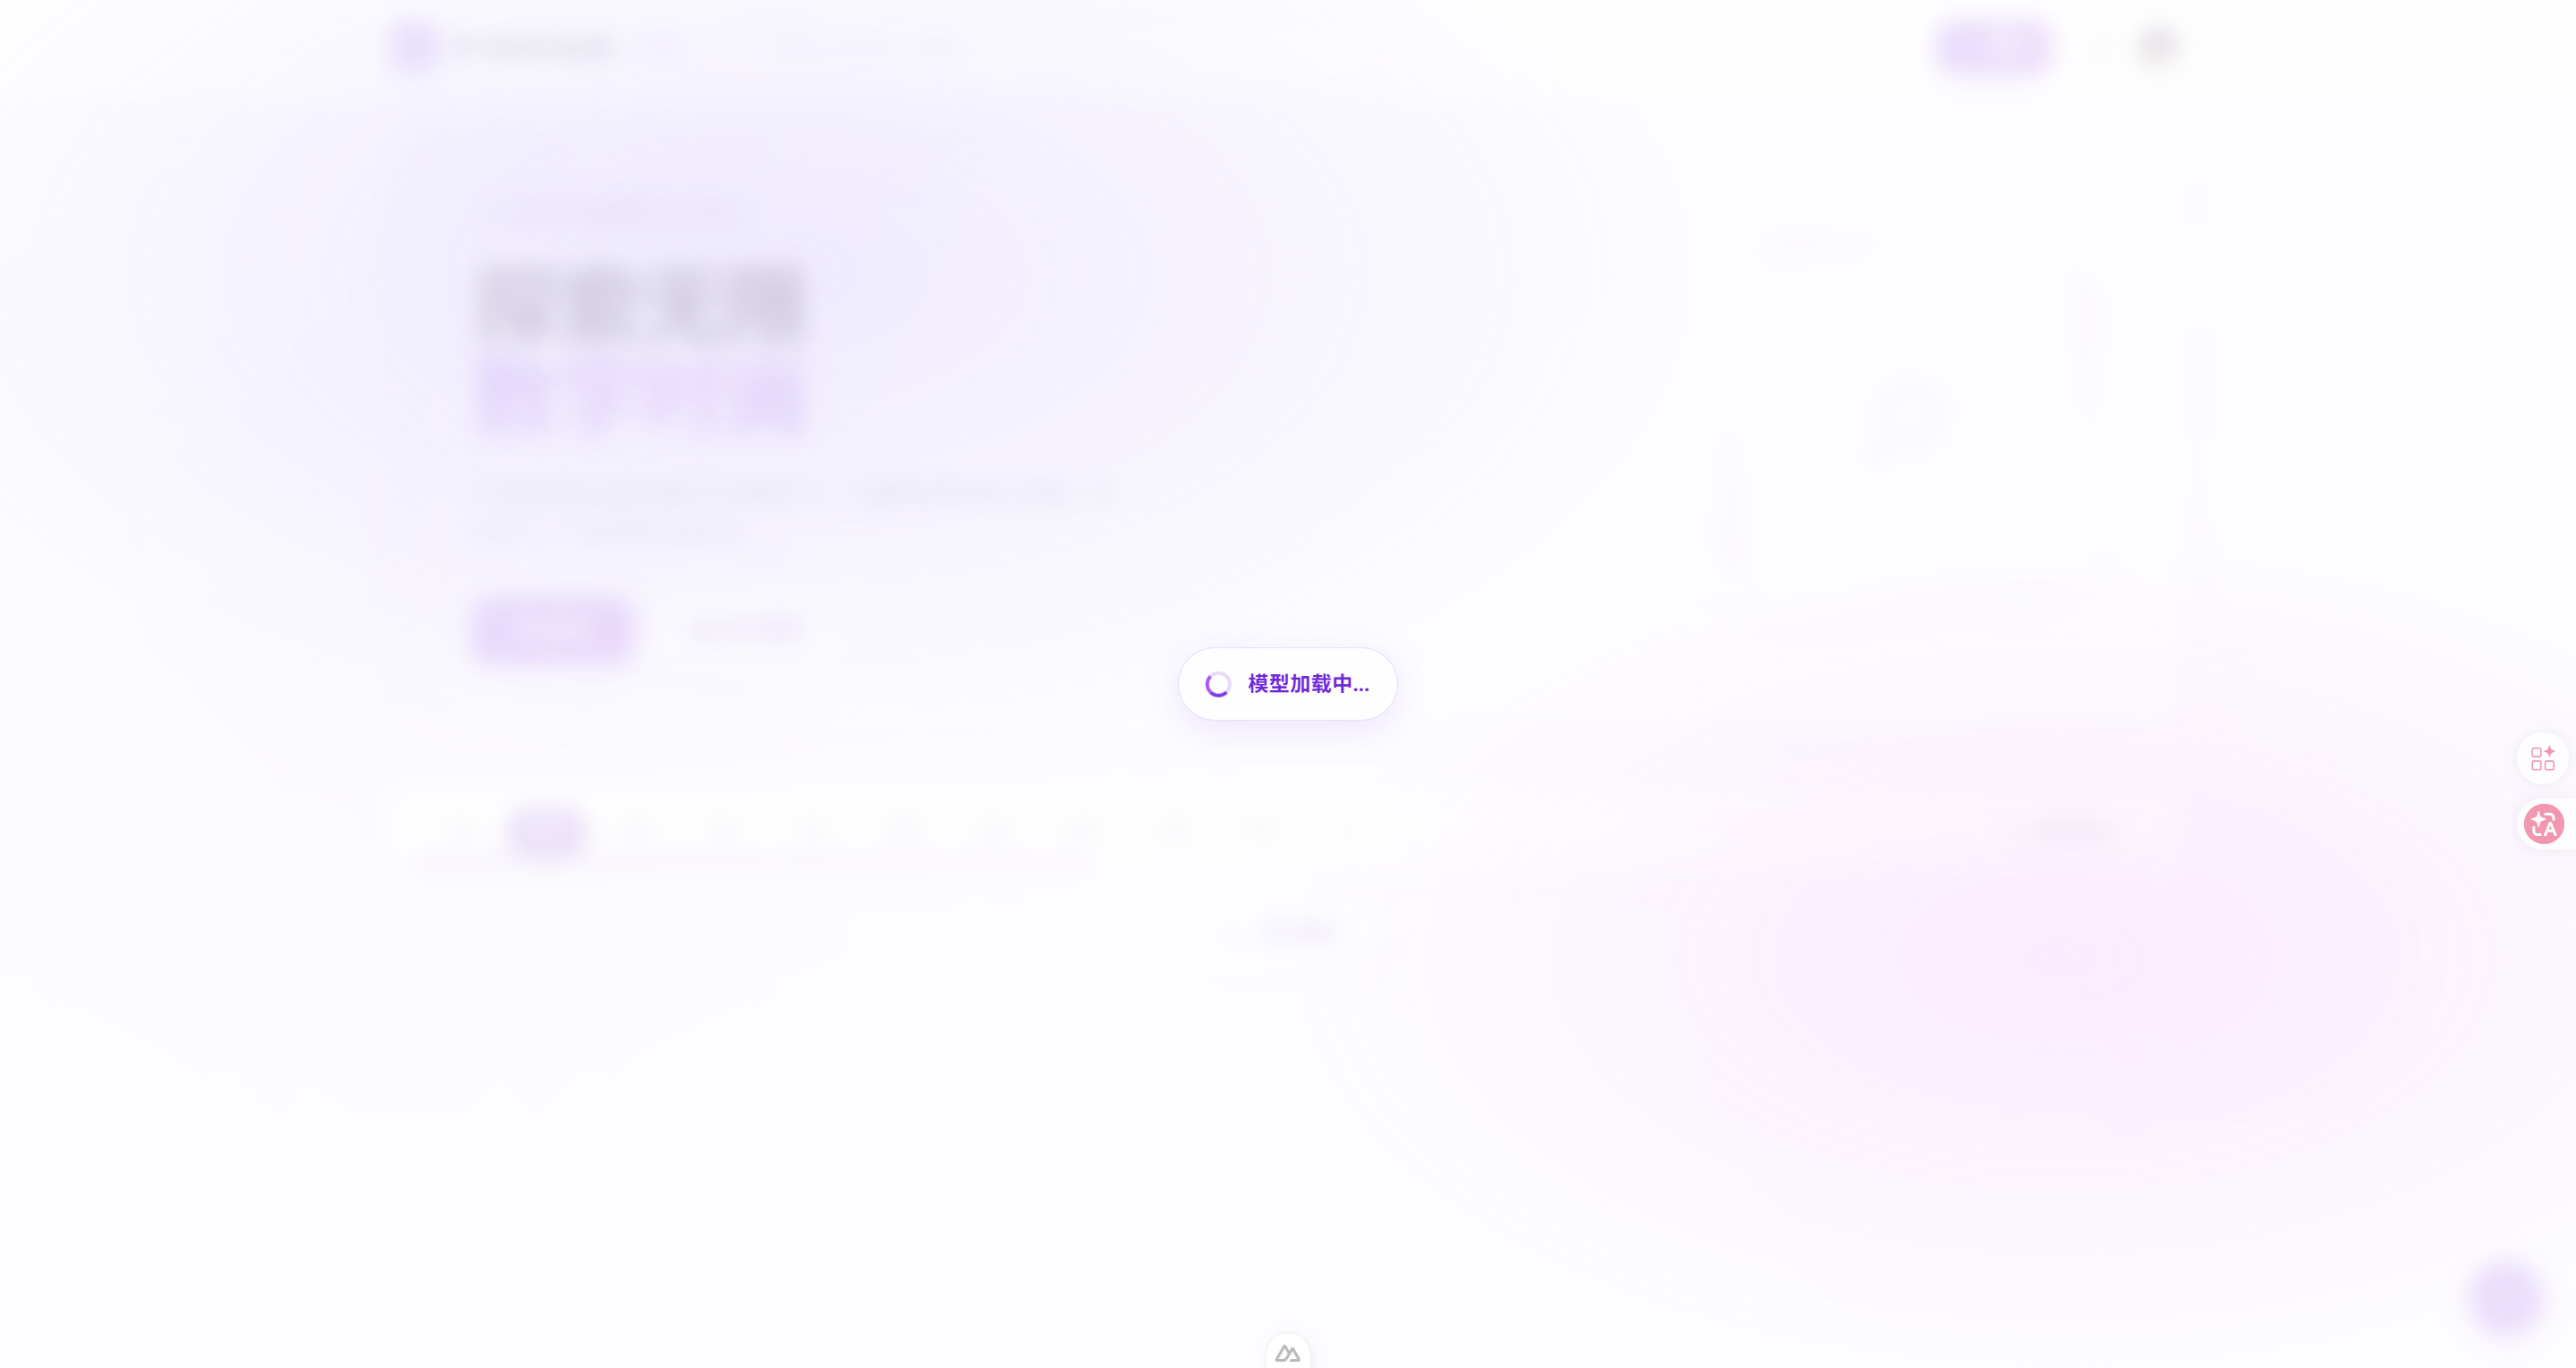
\includegraphics[width=0.85\textwidth]{test12}
	\caption{创意广场展示}
	\label{fig:test-creative-square}
\end{figure}

\subsubsection{搜索、筛选与排序}

测试用例如表~\ref{tab:testcase-square-search}所示。

\begin{table}[H]
	\centering
	\caption{搜索、筛选与排序测试用例}
	\label{tab:testcase-square-search}
	\renewcommand{\arraystretch}{1.25}
	\setlength{\tabcolsep}{0.2ex}
	\begin{tabularx}{\textwidth}{@{}>{\raggedright\arraybackslash}p{0.12\textwidth} >{\raggedright\arraybackslash}p{0.22\textwidth} >{\raggedright\arraybackslash}X >{\raggedright\arraybackslash}X@{}}
		\toprule
		\textbf{\mbox{用例ID}} & \textbf{\mbox{前置条件}} & \textbf{\mbox{测试步骤}} & \textbf{\mbox{期望结果}} \\
		\midrule
		\mbox{010} & 已登录；进入创意广场列表页。 & 1. 使用关键词搜索作品/用户；\newline 2. 使用标签/风格/时间等筛选条件组合查询；\newline 3. 清空筛选条件，检查列表是否恢复默认。 & 1. 搜索结果与筛选条件一致；\newline 2. 条件切换后列表更新及时，不出现条件叠加错误。 \\
		\bottomrule
	\end{tabularx}
\end{table}

测试结果与期望一致：关键词搜索与筛选结果匹配，条件切换后列表更新及时且不出现条件叠加错误。如图~\ref{fig:test-search}所示。

\begin{figure}[H]
	\centering
	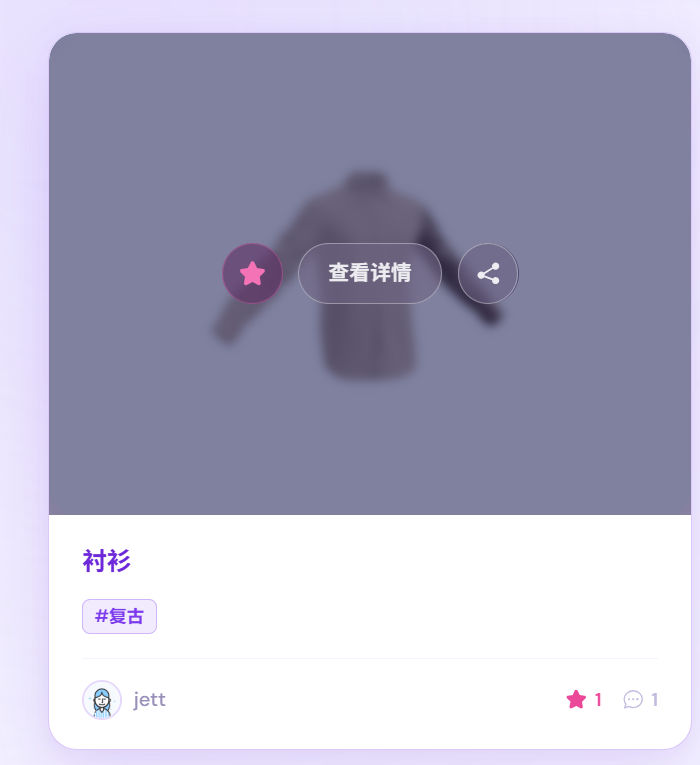
\includegraphics[width=0.85\textwidth]{test13}
	\caption{搜索加载展示}
	\label{fig:test-search}
\end{figure}

\subsubsection{互动与反馈}

测试用例如表~\ref{tab:testcase-square-interact}所示。

\begin{table}[H]
	\centering
	\caption{互动与反馈测试用例}
	\label{tab:testcase-square-interact}
	\renewcommand{\arraystretch}{1.25}
	\setlength{\tabcolsep}{0.2ex}
	\begin{tabularx}{\textwidth}{@{}>{\raggedright\arraybackslash}p{0.12\textwidth} >{\raggedright\arraybackslash}p{0.22\textwidth} >{\raggedright\arraybackslash}X >{\raggedright\arraybackslash}X@{}}
		\toprule
		\textbf{\mbox{用例ID}} & \textbf{\mbox{前置条件}} & \textbf{\mbox{测试步骤}} & \textbf{\mbox{期望结果}} \\
		\midrule
		\mbox{011} & 已登录；处于作品列表/作品详情或作者主页页面。 & 1. 点赞/收藏/评论/分享/关注作者（按系统实现）；\newline 2. 取消点赞/取消关注等反向操作，验证状态回滚。 & 1. 互动状态即时更新并在刷新后保持一致；\newline 2. 不允许的操作有明确提示（未登录、无权限、内容违规等）。 \\
		\bottomrule
	\end{tabularx}
\end{table}

测试结果与期望一致：点赞/收藏/评论/关注等互动状态可即时更新并在刷新后保持一致，取消操作可正确回滚；不允许的操作提示明确。结果如图~\ref{fig:test-work-interaction}和图~\ref{fig:test-author-home}所示。

\begin{figure}[H]
	\centering
	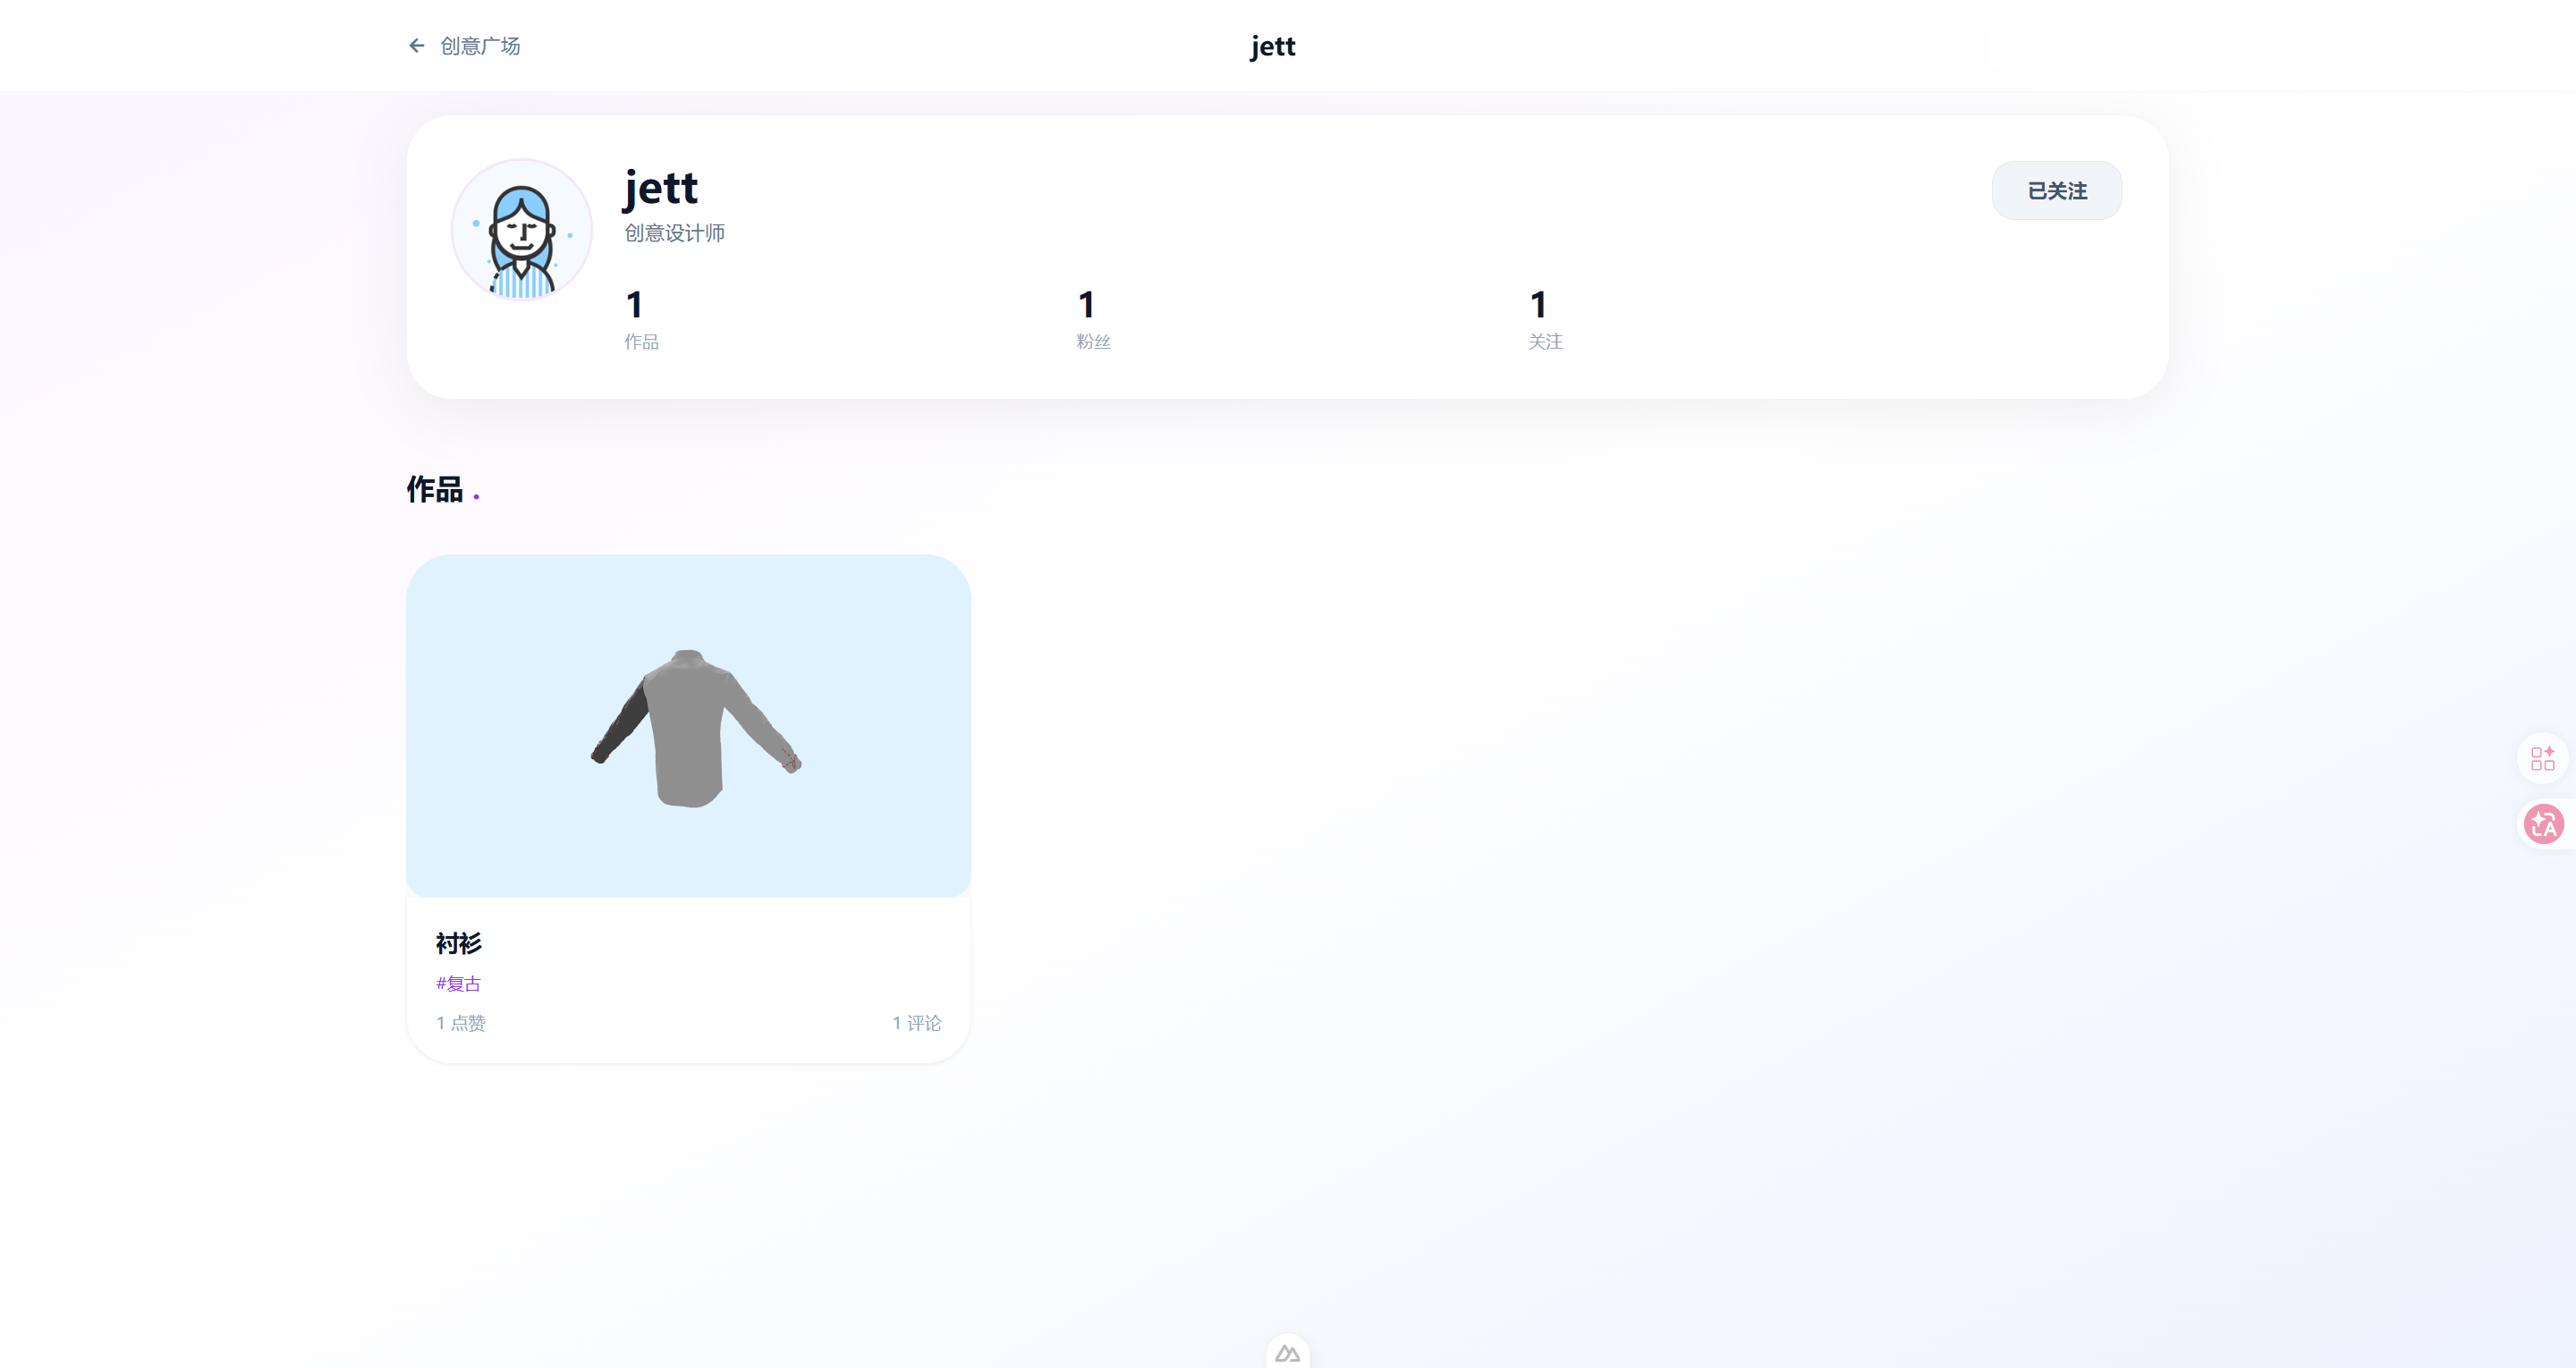
\includegraphics[width=0.85\textwidth]{test14}
	\caption{作品交互展示}
	\label{fig:test-work-interaction}
\end{figure}

\begin{figure}[H]
	\centering
	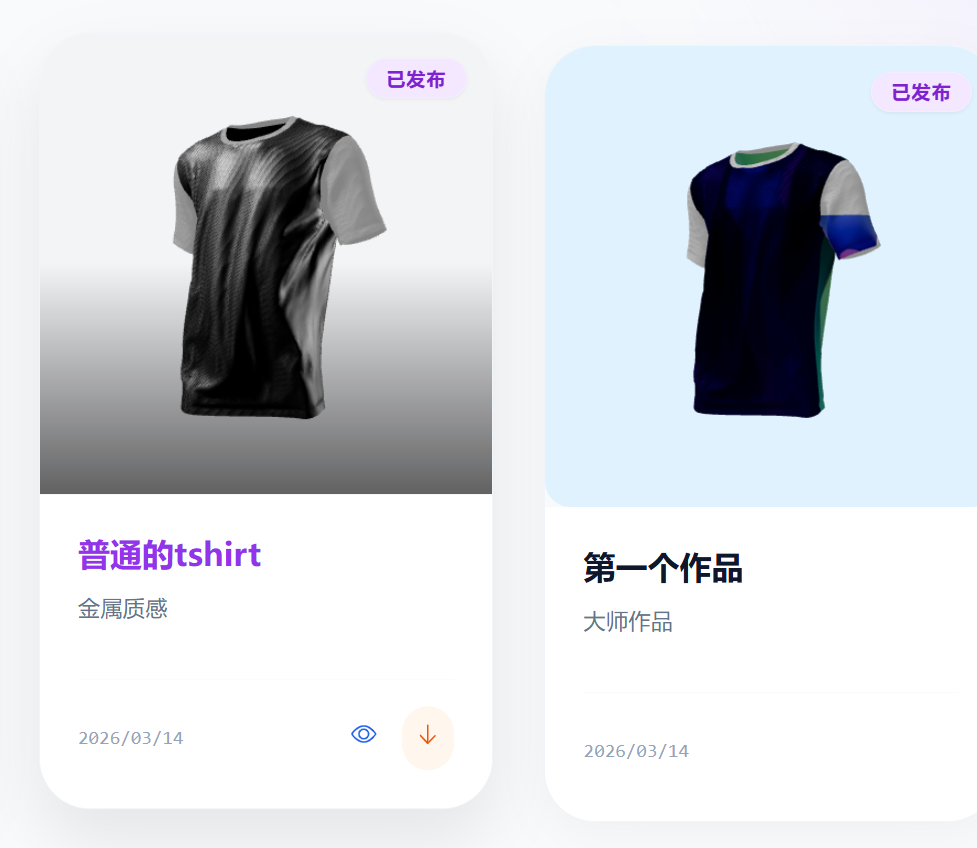
\includegraphics[width=0.85\textwidth]{test15}
	\caption{作者主页展示}
	\label{fig:test-author-home}
\end{figure}

\subsection{作品管理模块测试}

作品管理模块面向个人创作资产，主要覆盖作品创建、编辑、发布状态管理等流程，验证数据一致性与权限控制。

\subsubsection{作品创建与保存}

测试用例如表~\ref{tab:testcase-work-create}所示。

\begin{table}[H]
	\centering
	\caption{作品创建与保存测试用例}
	\label{tab:testcase-work-create}
	\renewcommand{\arraystretch}{1.25}
	\setlength{\tabcolsep}{0.2ex}
	\begin{tabularx}{\textwidth}{@{}>{\raggedright\arraybackslash}p{0.12\textwidth} >{\raggedright\arraybackslash}p{0.22\textwidth} >{\raggedright\arraybackslash}X >{\raggedright\arraybackslash}X@{}}
		\toprule
		\textbf{\mbox{用例ID}} & \textbf{\mbox{前置条件}} & \textbf{\mbox{测试步骤}} & \textbf{\mbox{期望结果}} \\
		\midrule
		\mbox{012} & 已登录。 & 1. 进入“我的作品”，新建作品；\newline 2. 保存为草稿，提交审核，验证发布流程是否正确。 & 1. 必填字段校验准确；保存成功后列表中可见该作品；\newline 2. 回显内容与保存内容一致（含图片、标签、关联资源）。 \\
		\bottomrule
	\end{tabularx}
\end{table}

测试结果与期望一致：必填字段校验准确，作品保存成功后可在“我的作品”列表中查看且回显信息一致，状态流转显示正常。如图~\ref{fig:test-mywork}所示。

\begin{figure}[H]
	\centering
	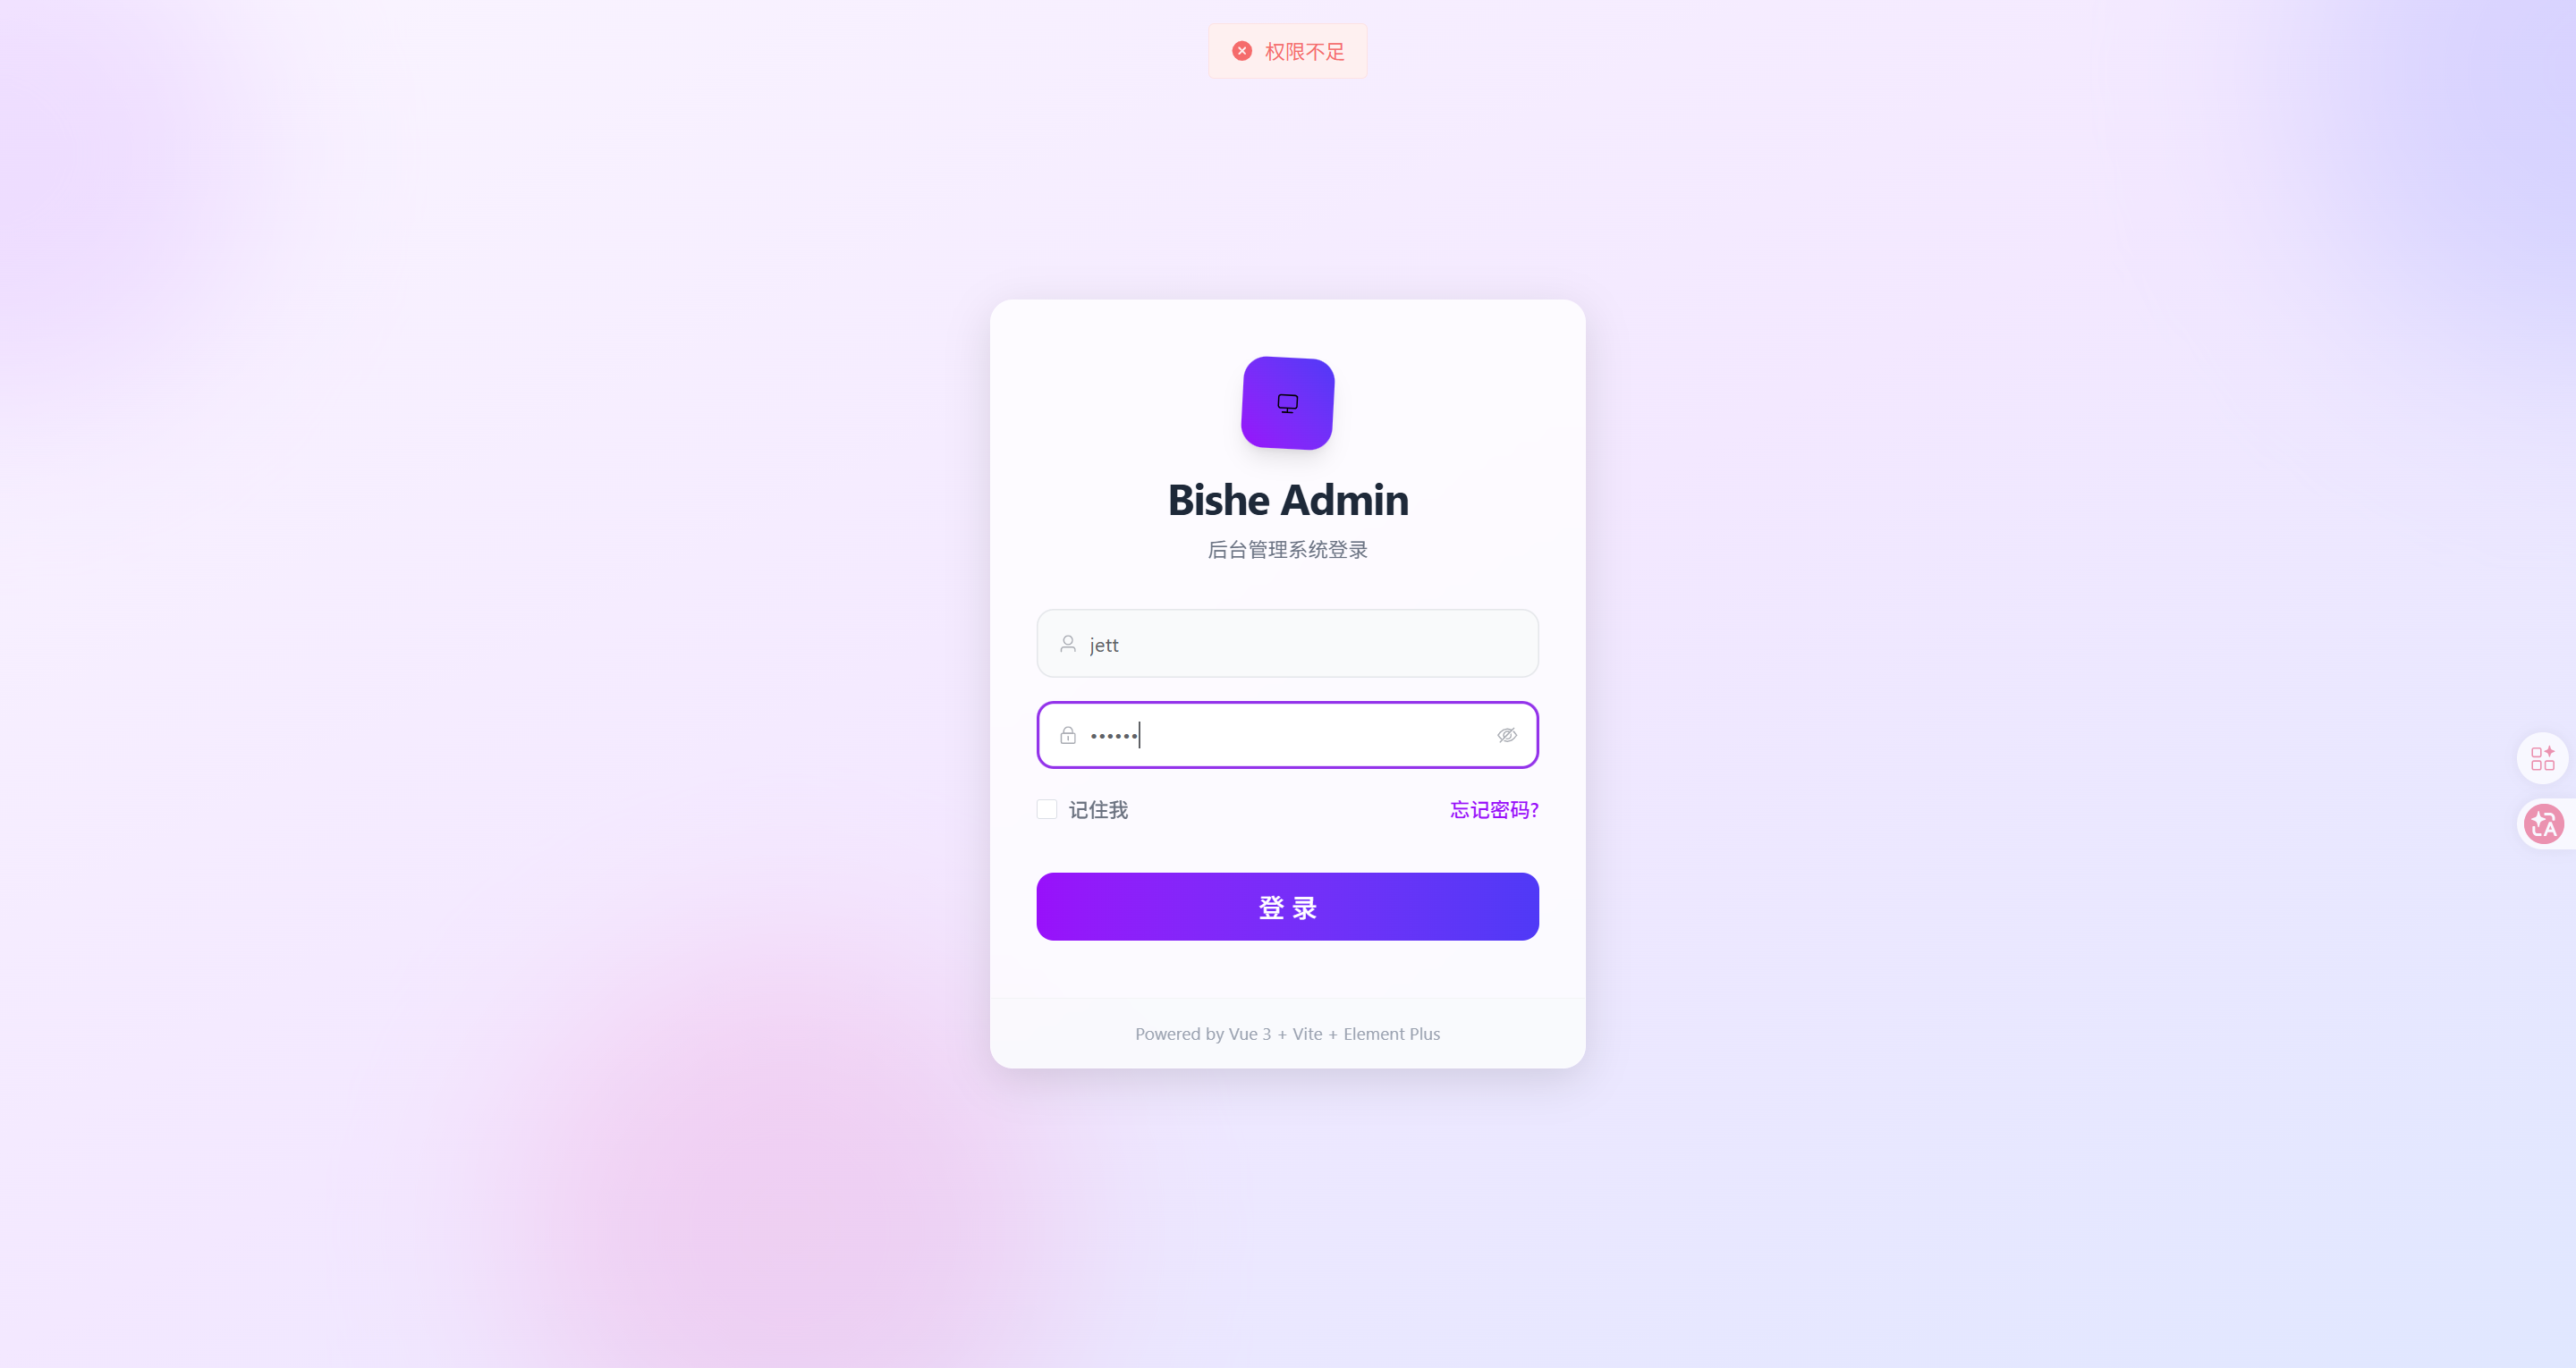
\includegraphics[width=0.85\textwidth]{test16}
	\caption{我的作品展示}
	\label{fig:test-mywork}
\end{figure}

\subsubsection{作品编辑、发布与撤回}

测试用例如表~\ref{tab:testcase-work-publish}所示。

\begin{table}[H]
	\centering
	\caption{作品编辑、发布与撤回测试用例}
	\label{tab:testcase-work-publish}
	\renewcommand{\arraystretch}{1.25}
	\setlength{\tabcolsep}{0.2ex}
	\begin{tabularx}{\textwidth}{@{}>{\raggedright\arraybackslash}p{0.12\textwidth} >{\raggedright\arraybackslash}p{0.22\textwidth} >{\raggedright\arraybackslash}X >{\raggedright\arraybackslash}X@{}}
		\toprule
		\textbf{\mbox{用例ID}} & \textbf{\mbox{前置条件}} & \textbf{\mbox{测试步骤}} & \textbf{\mbox{期望结果}} \\
		\midrule
		\mbox{013} & 作品已存在。 & 1. 编辑作品信息并保存，检查更新是否生效；\newline 2. 发布作品到创意广场（如有），在广场侧确认可见性；\newline 3. 撤回/下架作品（如有），验证广场端不可见且个人端状态正确。 & 1. 发布状态切换正确；不同状态下可执行的操作按钮符合权限（如草稿可编辑，已发布可下架等）。 \\
		\bottomrule
	\end{tabularx}
\end{table}

测试结果与期望一致：作品发布、撤回/下架等状态切换正确，不同状态下可执行操作与权限匹配且展示一致。如图~\ref{fig:test-work-publish-status}所示。

\begin{figure}[H]
	\centering
	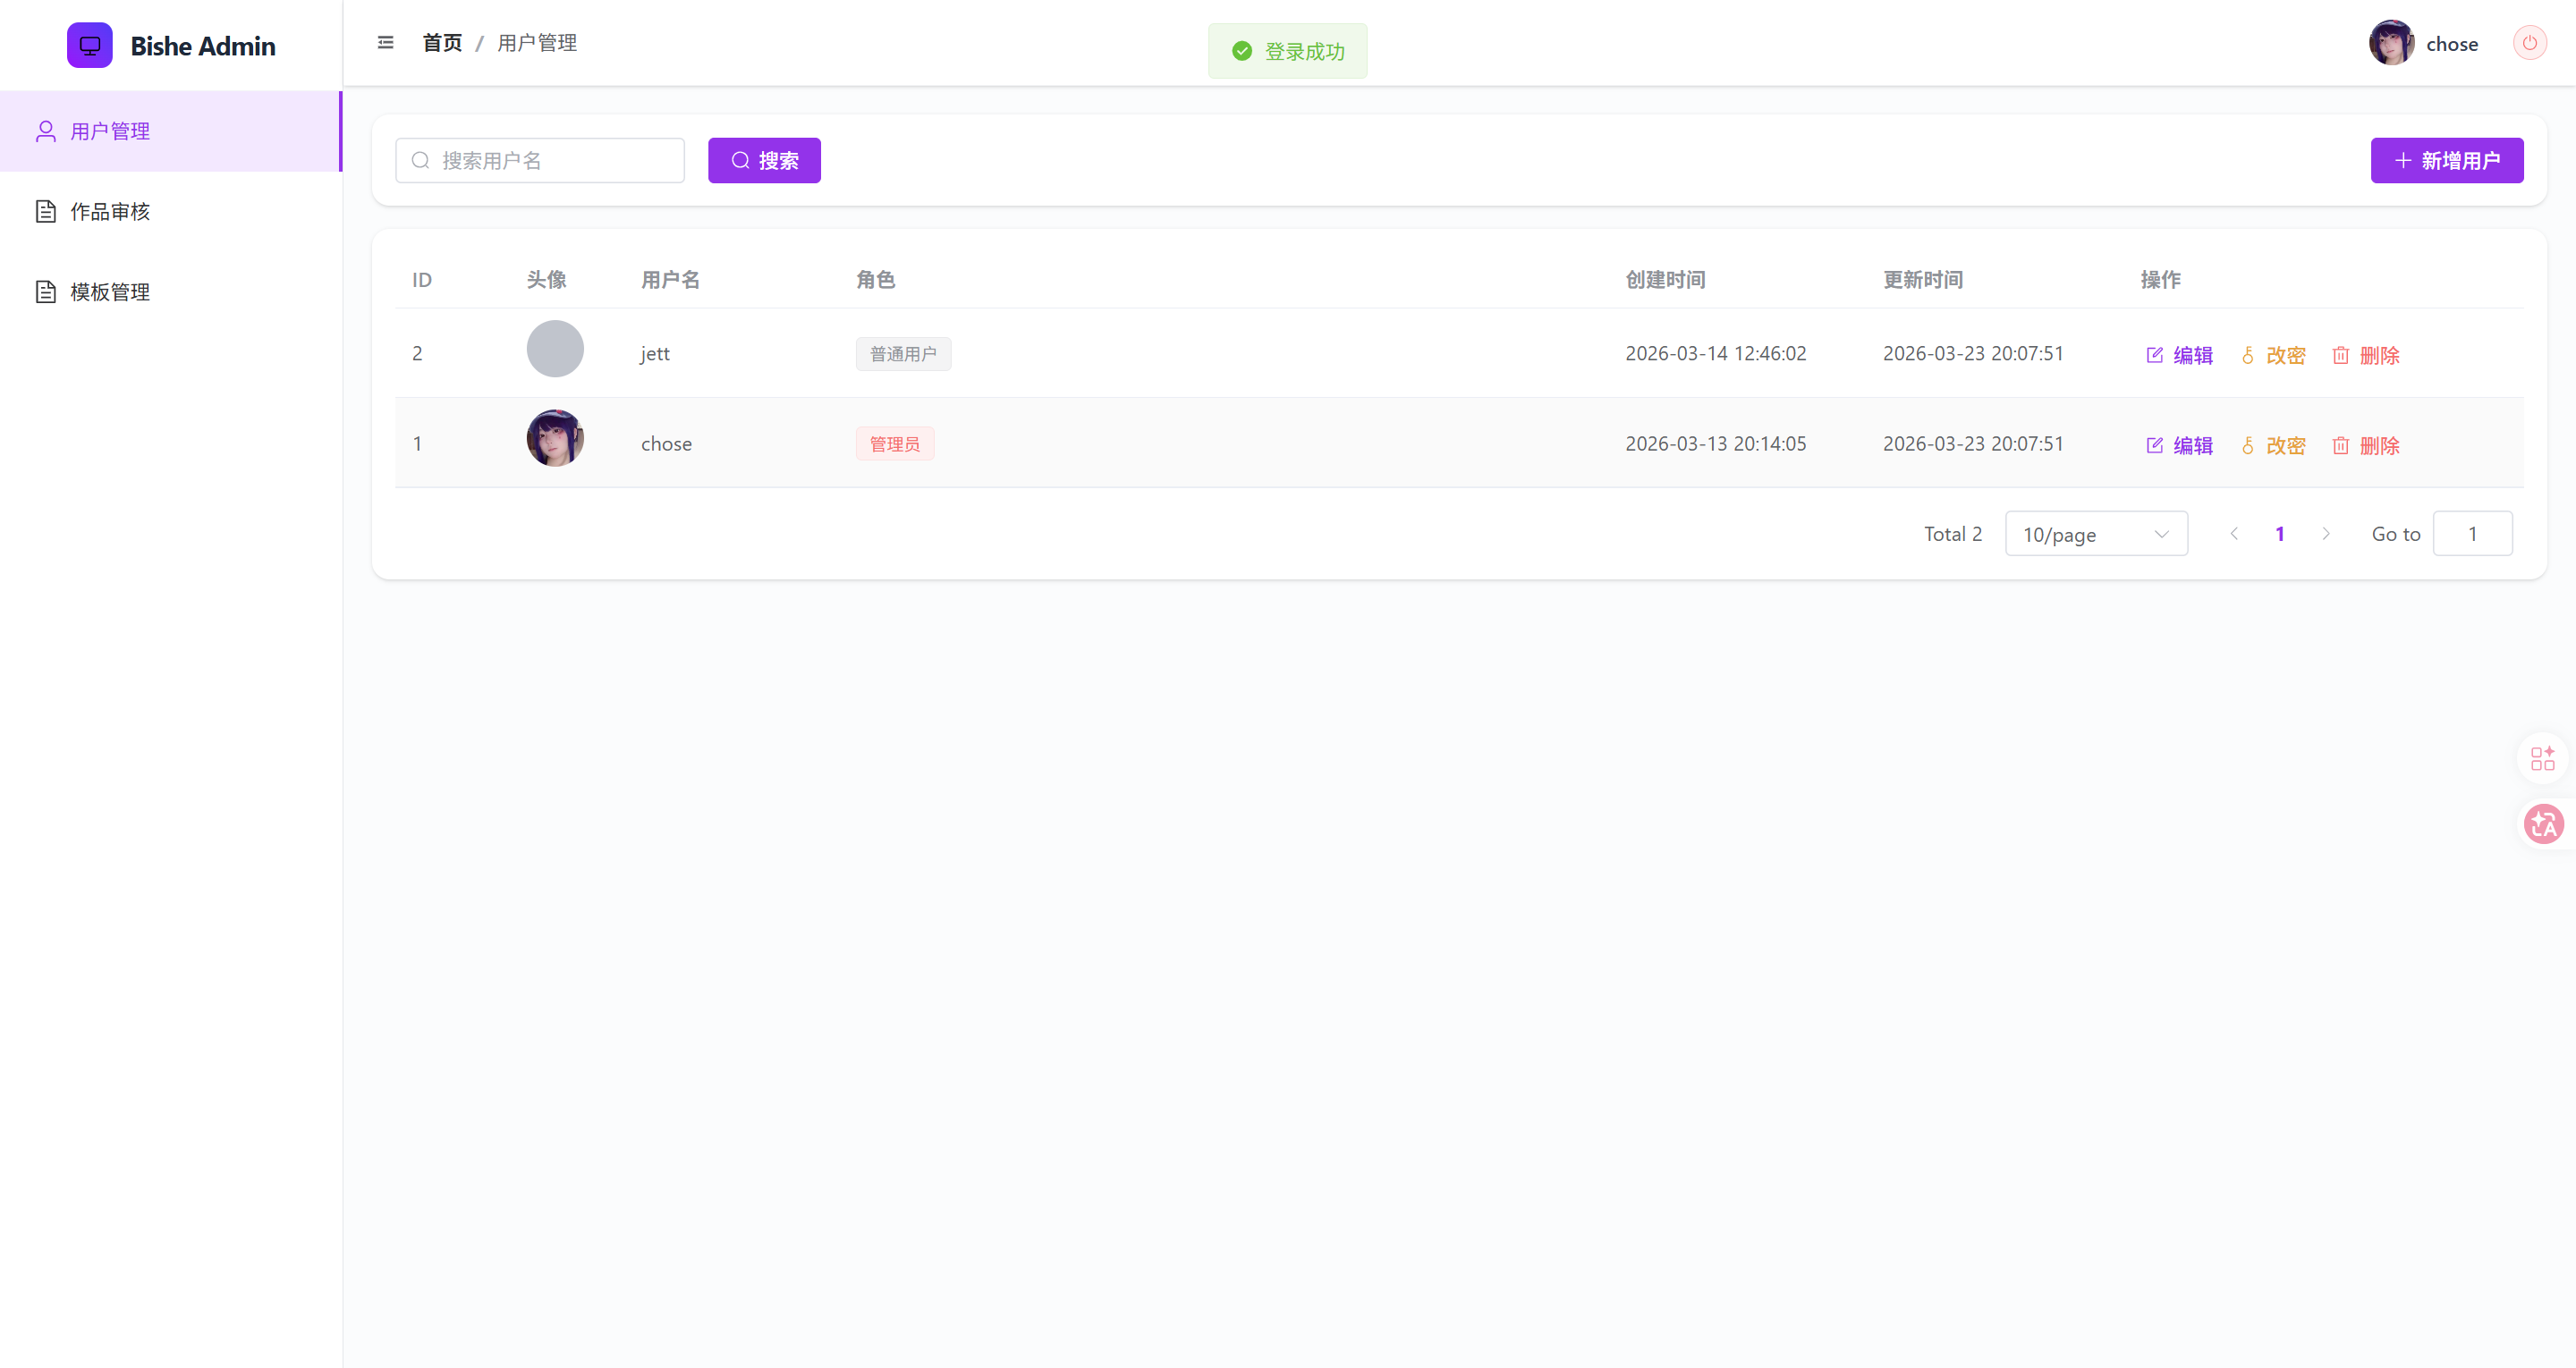
\includegraphics[width=0.85\textwidth]{test17}
	\caption{作品状态展示}
	\label{fig:test-work-publish-status}
\end{figure}

\subsection{后台管理模块测试}

后台管理模块主要覆盖管理员登录、用户管理、作品审核、模型管理等功能，验证管理操作的安全性与可追溯性。

\subsubsection{管理员登录与权限控制}

测试用例如表~\ref{tab:testcase-admin-login}所示。

\begin{table}[H]
	\centering
	\caption{管理员登录与权限控制测试用例}
	\label{tab:testcase-admin-login}
	\renewcommand{\arraystretch}{1.25}
	\setlength{\tabcolsep}{0.2ex}
	\begin{tabularx}{\textwidth}{@{}>{\raggedright\arraybackslash}p{0.12\textwidth} >{\raggedright\arraybackslash}p{0.22\textwidth} >{\raggedright\arraybackslash}X >{\raggedright\arraybackslash}X@{}}
		\toprule
		\textbf{\mbox{用例ID}} & \textbf{\mbox{前置条件}} & \textbf{\mbox{测试步骤}} & \textbf{\mbox{期望结果}} \\
		\midrule
		\mbox{014} & 管理员账号已配置。 & 1. 进入后台登录页，使用管理员账号登录；\newline 2. 使用普通用户账号尝试访问后台路由/页面，验证访问限制；\newline 3. 退出登录后再次访问后台页面，验证会话失效。 & 1. 仅管理员可访问后台；非管理员访问会被拦截并提示无权限或跳转登录。 \\
		\bottomrule
	\end{tabularx}
\end{table}

测试结果与期望一致：仅管理员可访问后台管理端，非管理员访问会被拦截并提示无权限或跳转登录；退出后会话失效需重新认证。结果如图~\ref{fig:test-admin-block}和图~\ref{fig:test-admin-login-success}所示。

\begin{figure}[H]
	\centering
	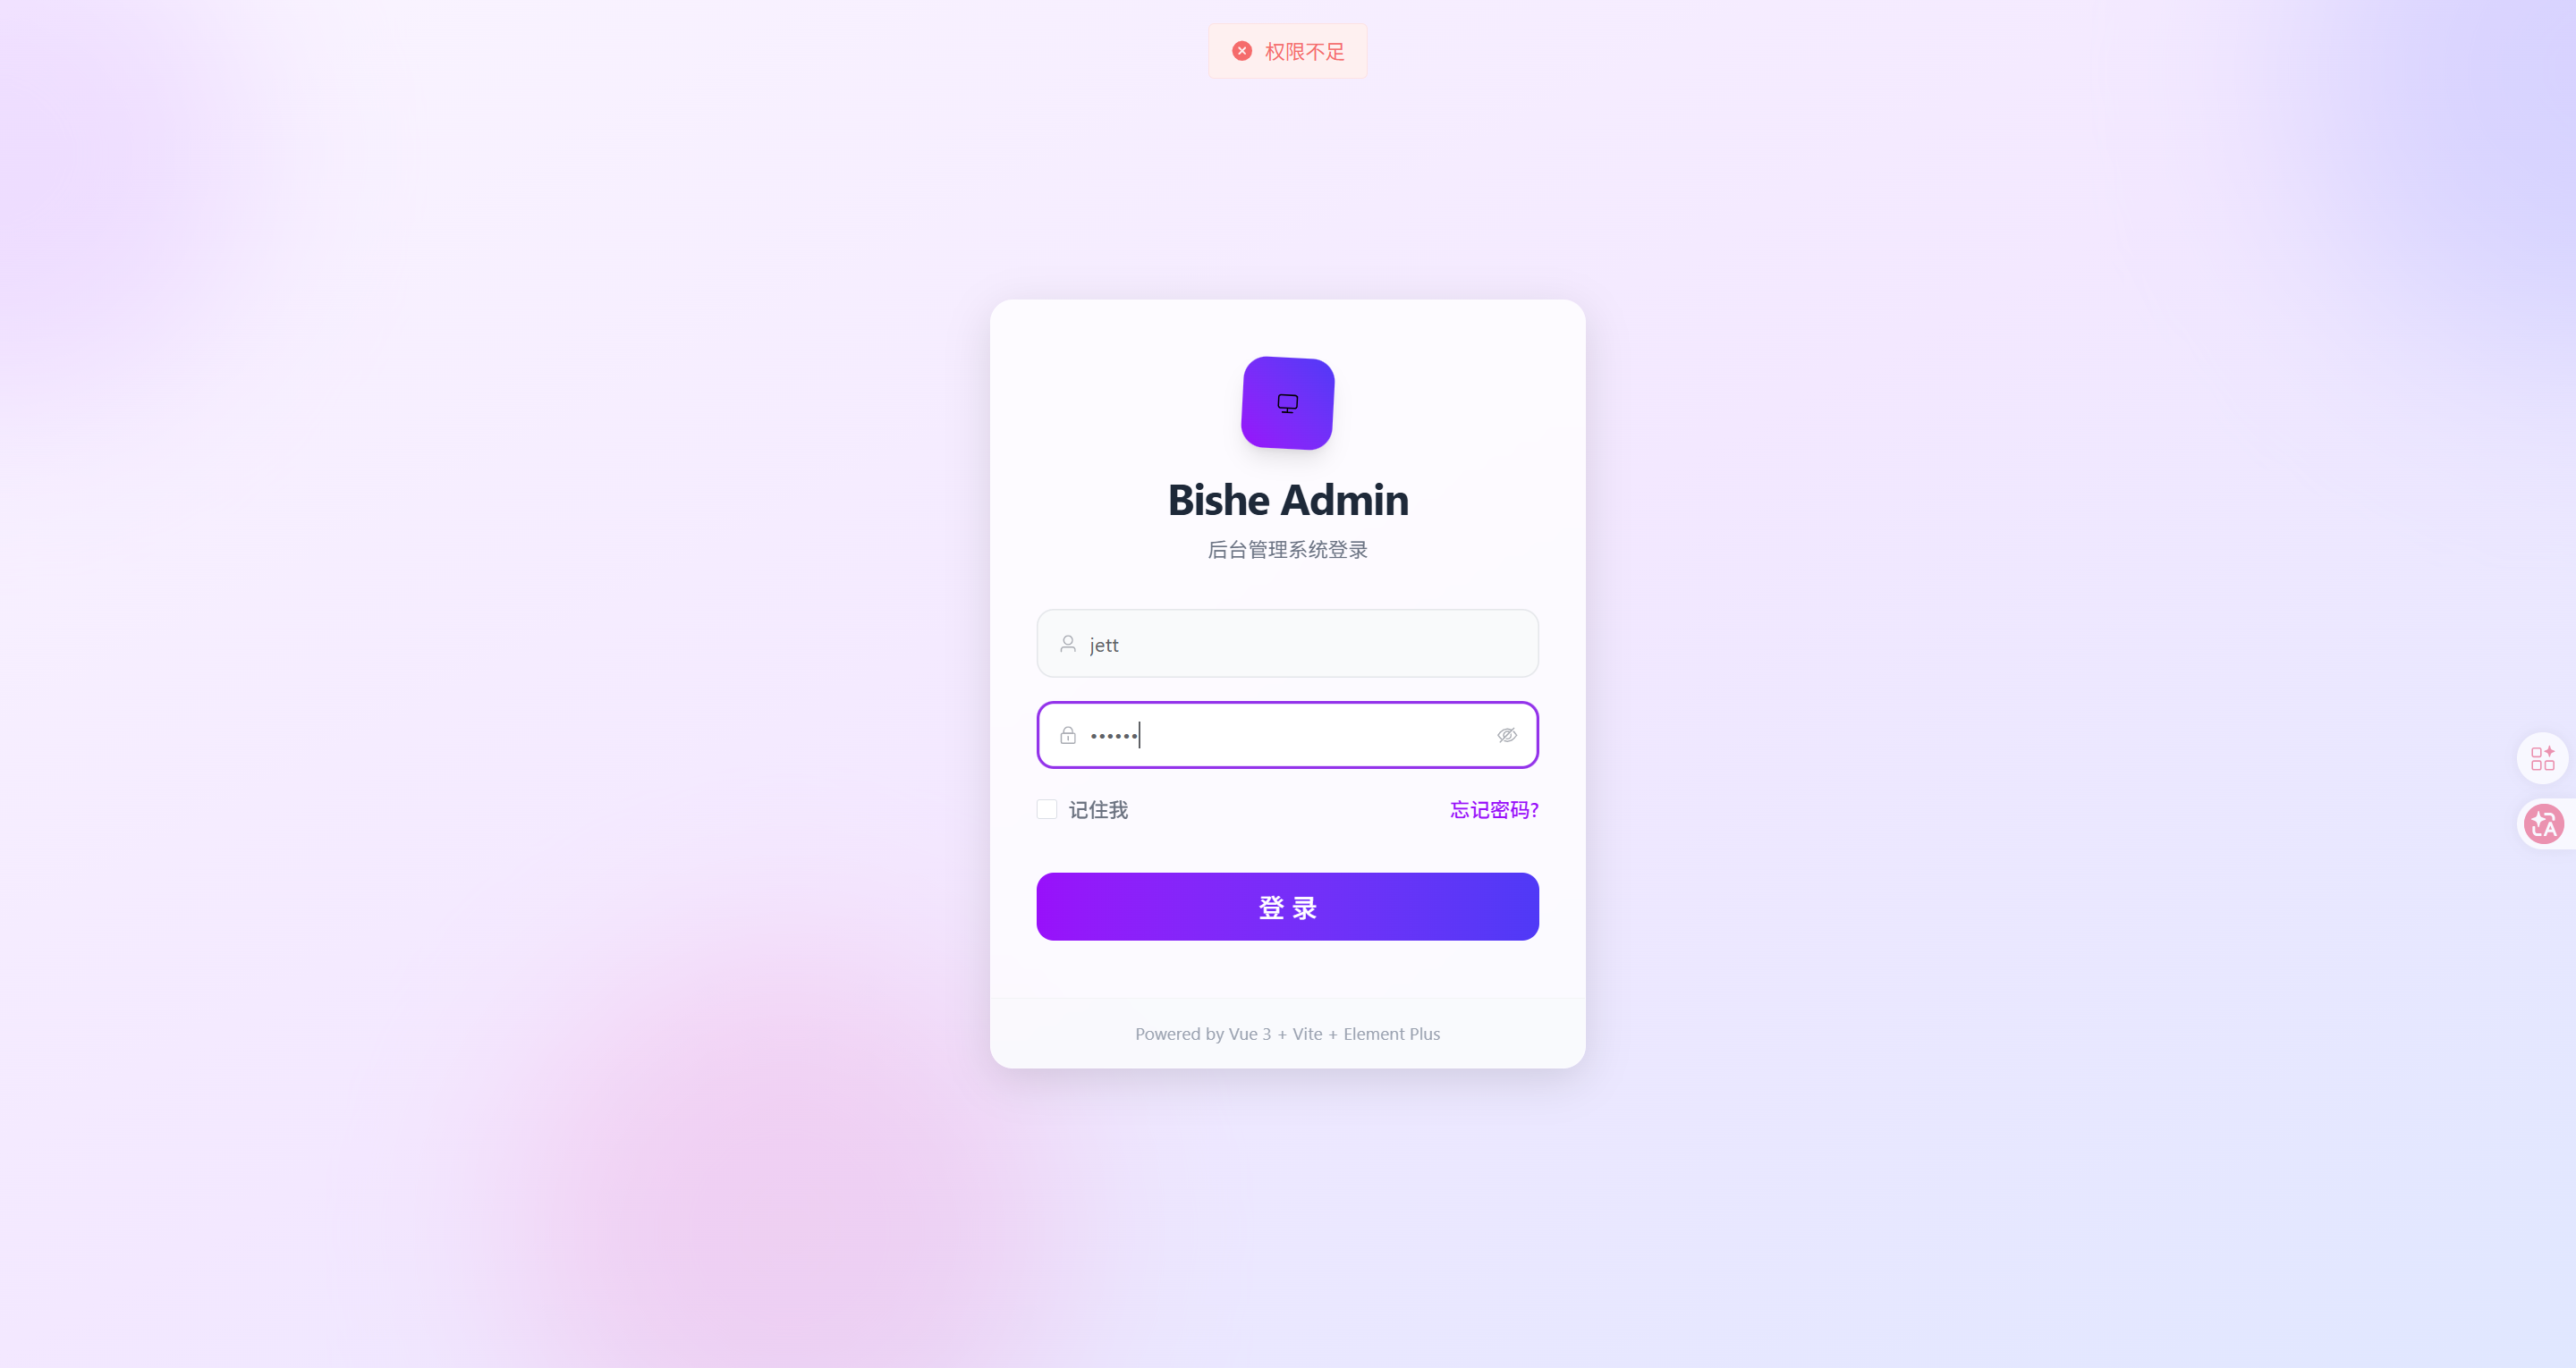
\includegraphics[width=0.85\textwidth]{test18}
	\caption{后台登录拦截展示}
	\label{fig:test-admin-block}
\end{figure}

\begin{figure}[H]
	\centering
	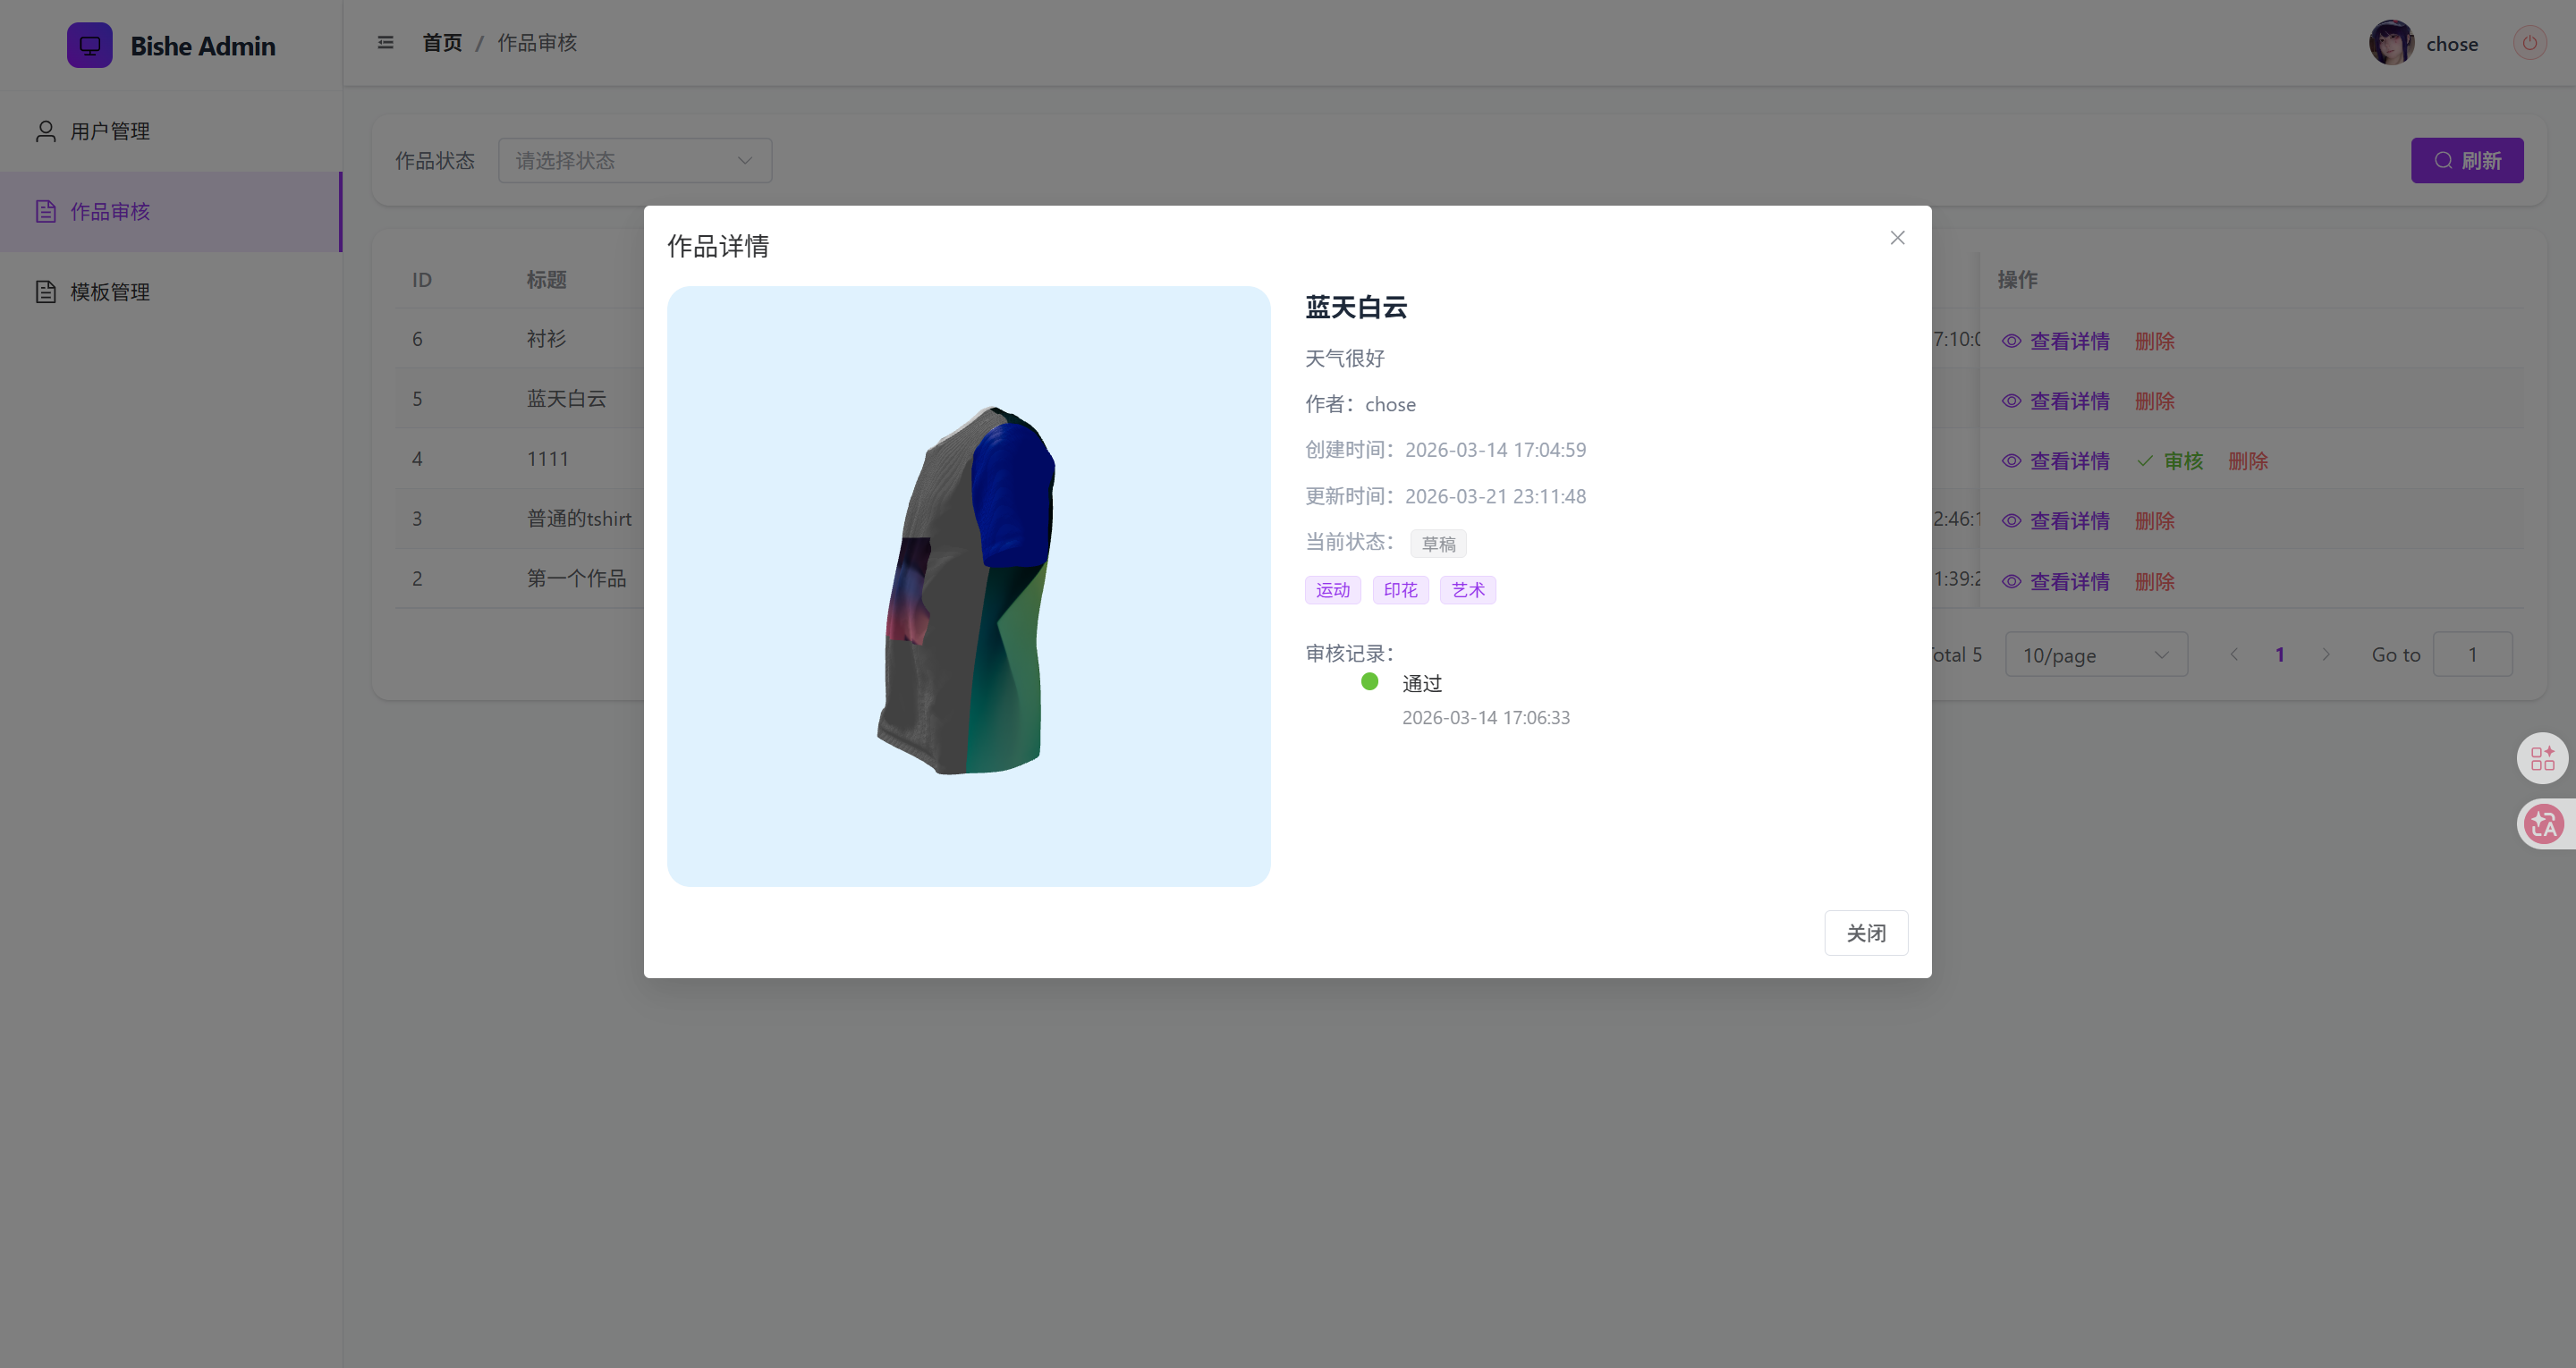
\includegraphics[width=0.85\textwidth]{test19}
	\caption{后台登录成功展示}
	\label{fig:test-admin-login-success}
\end{figure}

\subsubsection{用户管理}

测试用例如表~\ref{tab:testcase-admin-user}所示。

\begin{table}[H]
	\centering
	\caption{用户管理测试用例}
	\label{tab:testcase-admin-user}
	\renewcommand{\arraystretch}{1.25}
	\setlength{\tabcolsep}{0.2ex}
	\begin{tabularx}{\textwidth}{@{}>{\raggedright\arraybackslash}p{0.12\textwidth} >{\raggedright\arraybackslash}p{0.22\textwidth} >{\raggedright\arraybackslash}X >{\raggedright\arraybackslash}X@{}}
		\toprule
		\textbf{\mbox{用例ID}} & \textbf{\mbox{前置条件}} & \textbf{\mbox{测试步骤}} & \textbf{\mbox{期望结果}} \\
		\midrule
		\mbox{015} & 已登录后台管理端，具备管理员权限。 & 1. 查询用户列表；\newline 2. 执行修改信息/密码/删除等管理动作，观察实际效果。 & 1. 管理操作有二次确认与结果提示；列表状态刷新正确。 \\
		\bottomrule
	\end{tabularx}
\end{table}

测试结果与期望一致：用户列表查询正常，修改信息等管理操作具备二次确认与结果提示，列表刷新与数据回显一致。结果如图~\ref{fig:test-admin-user-list}和图~\ref{fig:test-admin-user-edit}所示。

\begin{figure}[H]
	\centering
	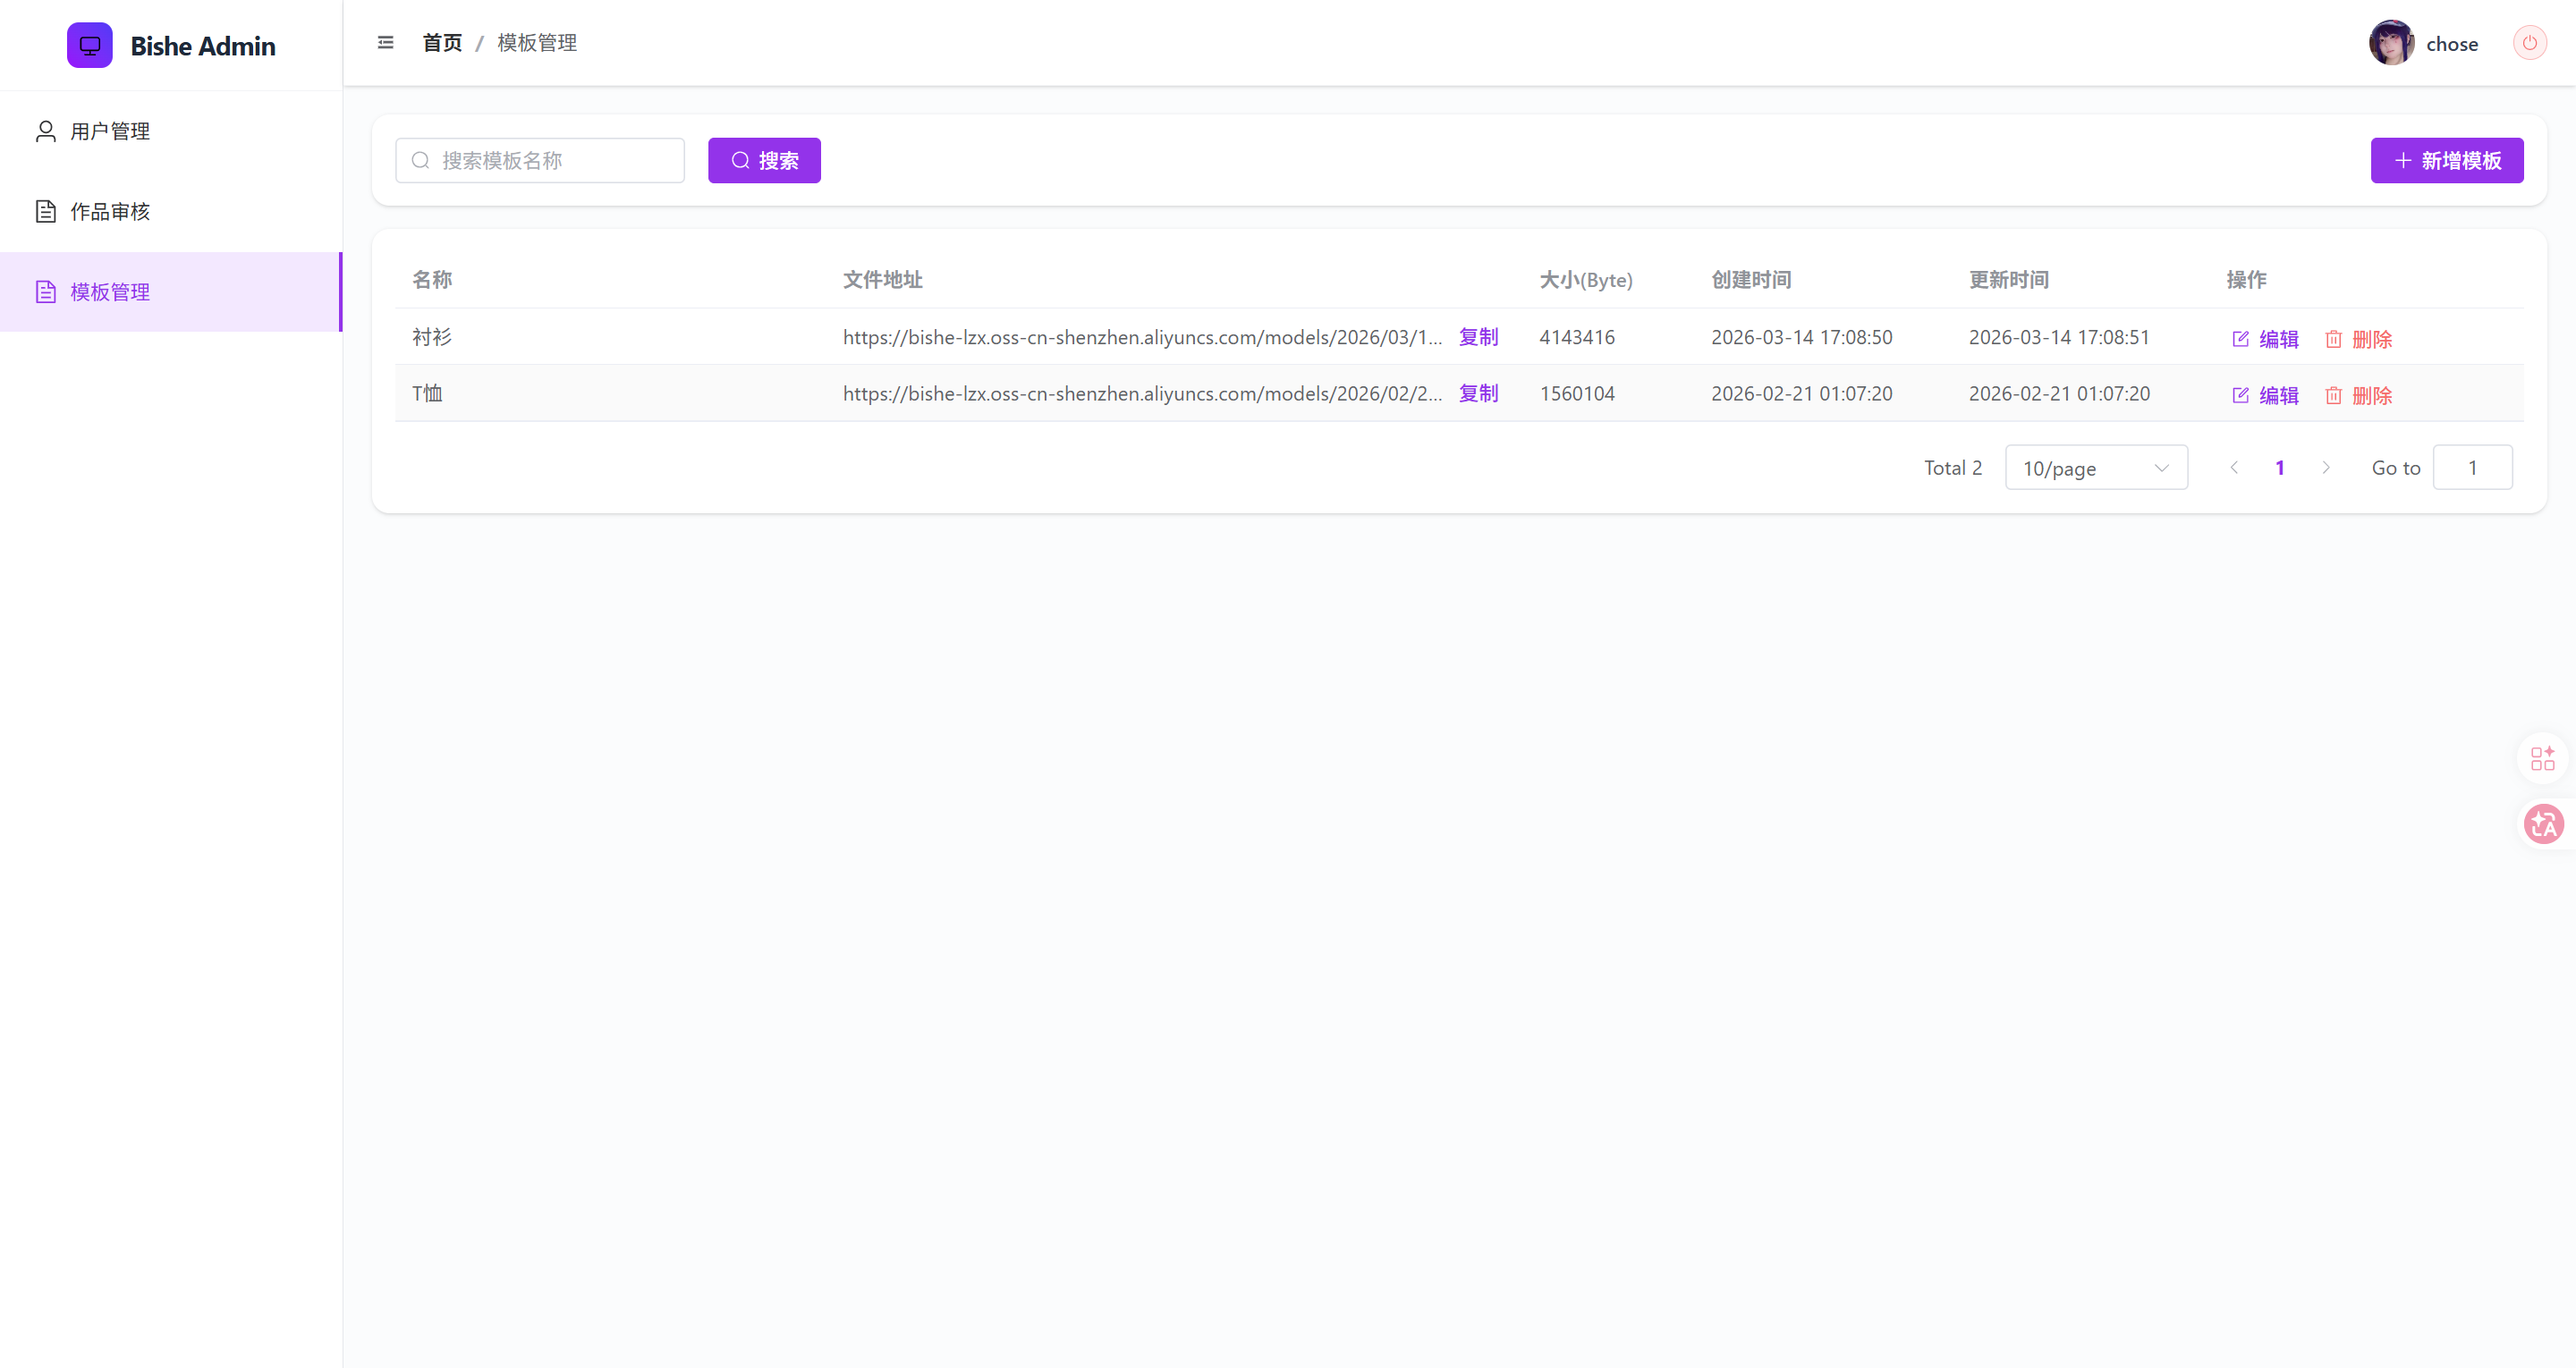
\includegraphics[width=0.85\textwidth]{test20}
	\caption{用户列表展示}
	\label{fig:test-admin-user-list}
\end{figure}

\begin{figure}[H]
	\centering
	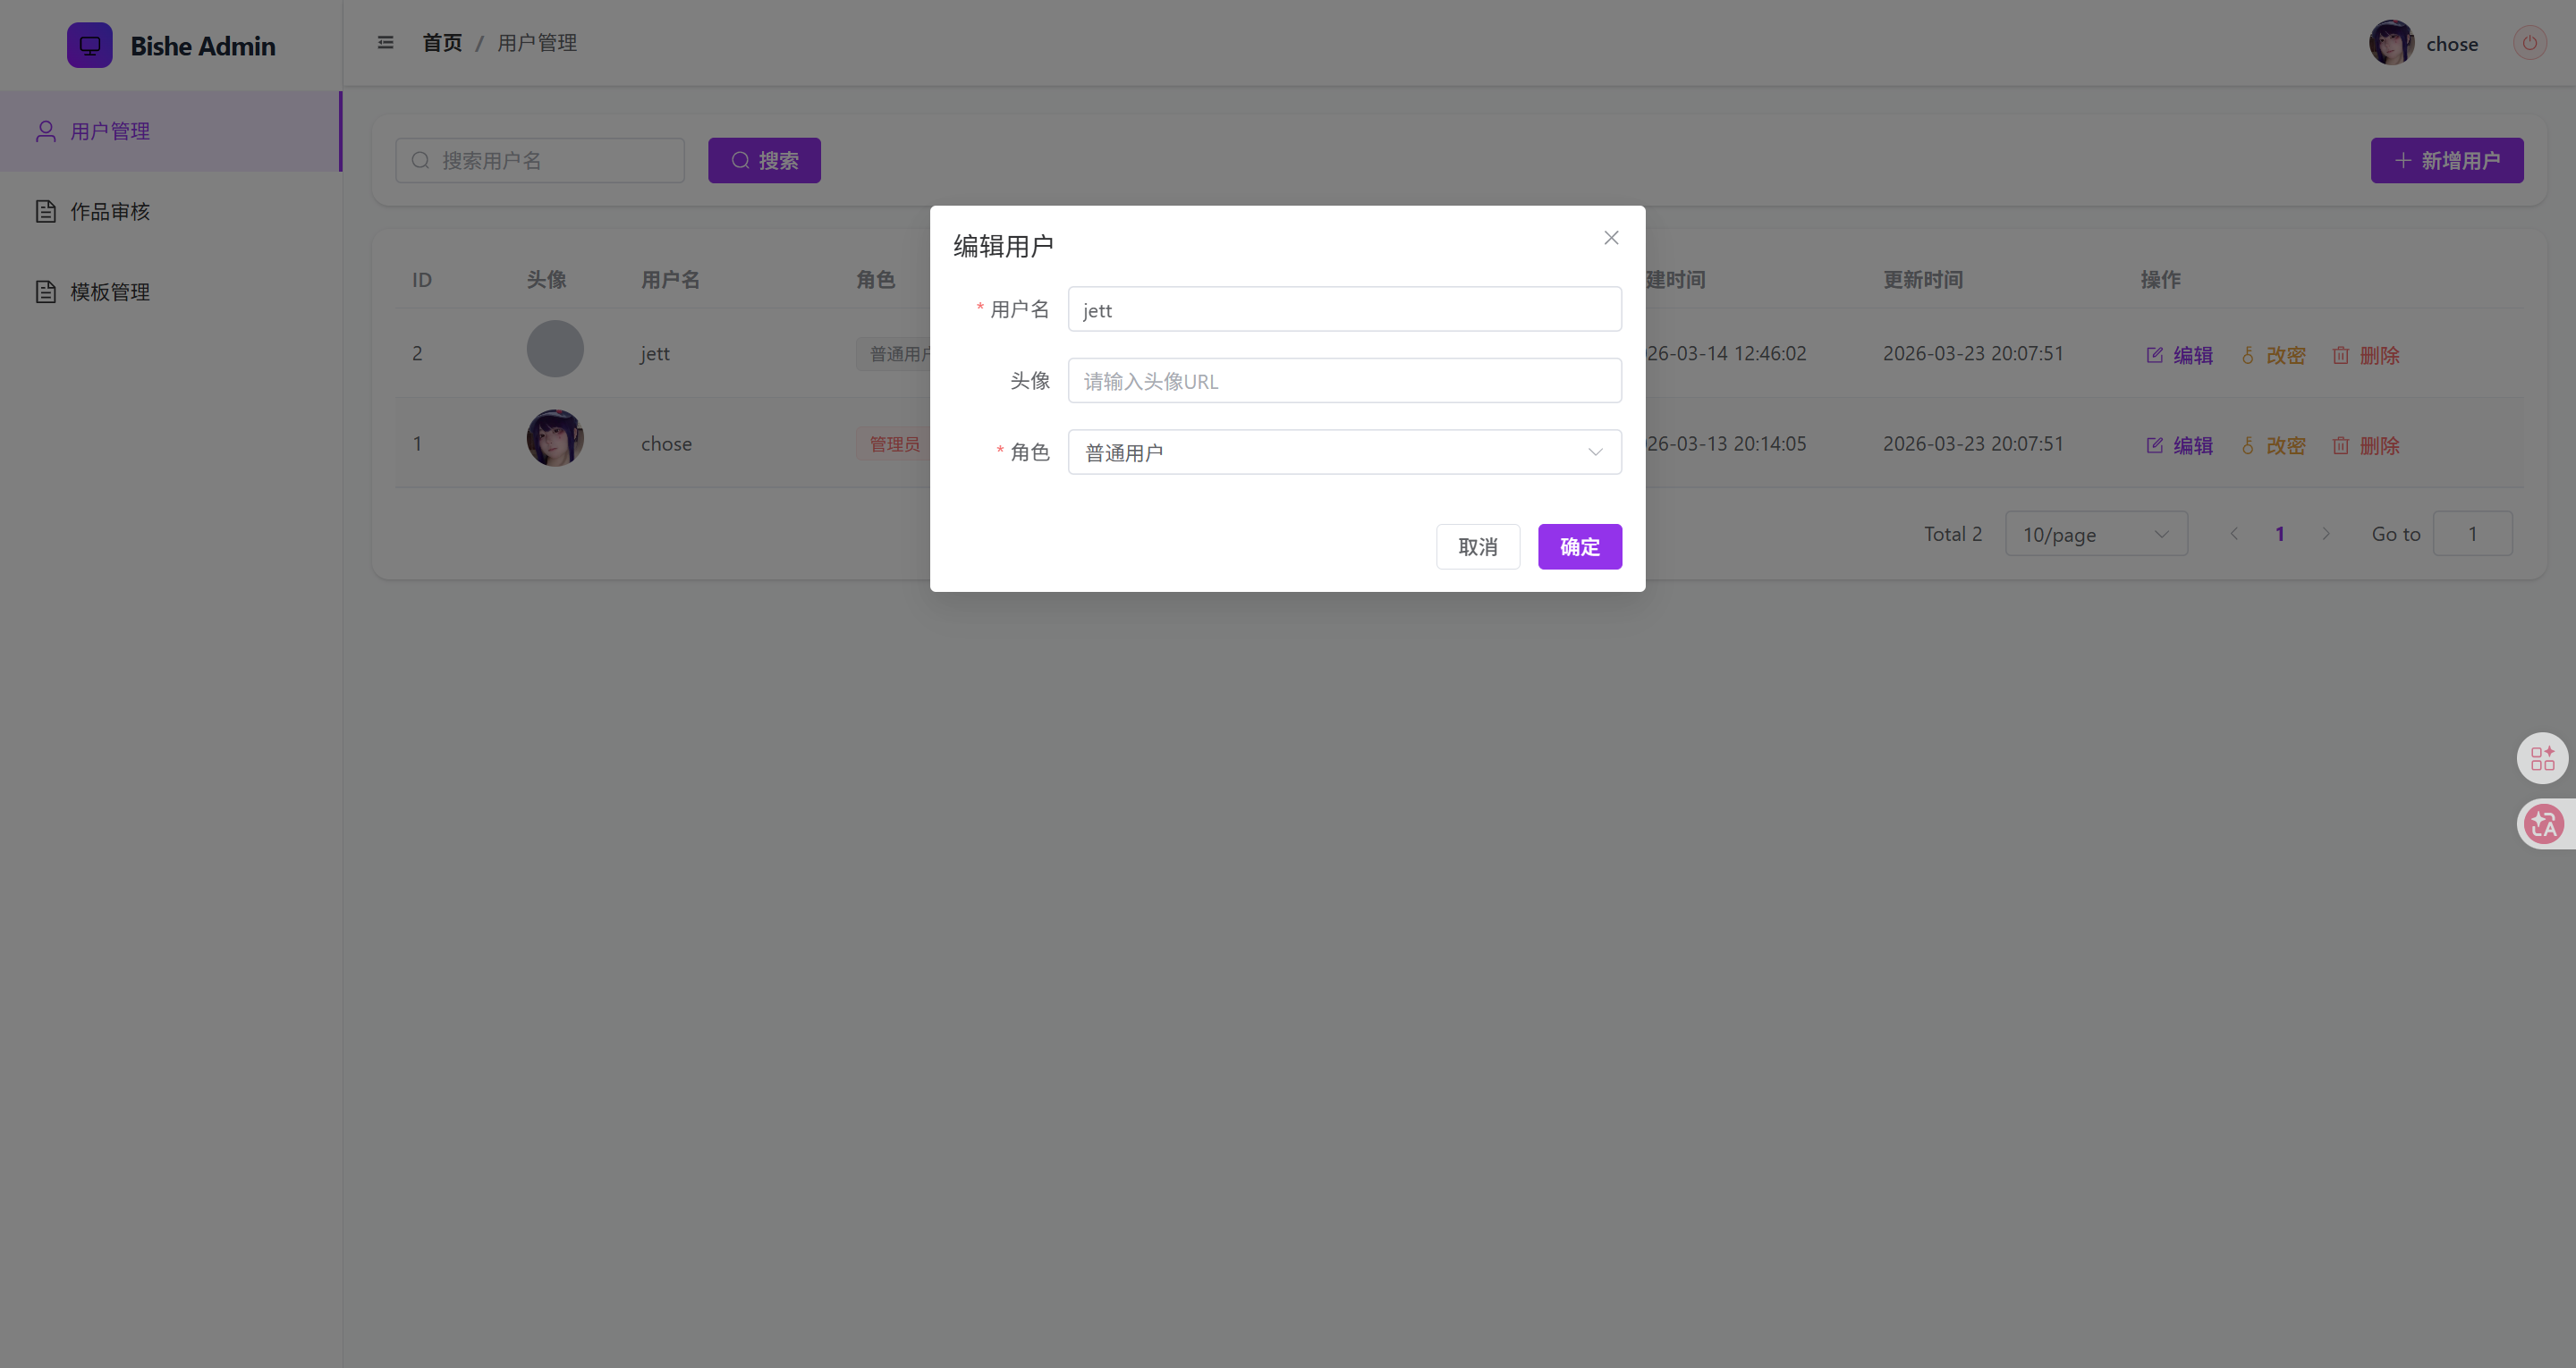
\includegraphics[width=0.85\textwidth]{test21}
	\caption{修改用户信息展示}
	\label{fig:test-admin-user-edit}
\end{figure}

\subsubsection{作品审核}

测试用例如表~\ref{tab:testcase-admin-review}所示。

\begin{table}[H]
	\centering
	\caption{作品审核测试用例}
	\label{tab:testcase-admin-review}
	\renewcommand{\arraystretch}{1.25}
	\setlength{\tabcolsep}{0.2ex}
	\begin{tabularx}{\textwidth}{@{}>{\raggedright\arraybackslash}p{0.12\textwidth} >{\raggedright\arraybackslash}p{0.22\textwidth} >{\raggedright\arraybackslash}X >{\raggedright\arraybackslash}X@{}}
		\toprule
		\textbf{\mbox{用例ID}} & \textbf{\mbox{前置条件}} & \textbf{\mbox{测试步骤}} & \textbf{\mbox{期望结果}} \\
		\midrule
		\mbox{016} & 已登录后台管理端；存在待审核作品。 & 1. 审核作品内容：通过、驳回、下架，检查前台展示变化。 & 1. 审核状态与前台可见性一致；驳回原因可记录并对作者可见（如系统支持）。 \\
		\bottomrule
	\end{tabularx}
\end{table}

测试结果与期望一致：作品审核通过/驳回/下架等操作生效，审核状态与前台可见性保持一致（如支持驳回原因记录，作者侧可见）。如图~\ref{fig:test-admin-review}所示。

\begin{figure}[H]
	\centering
	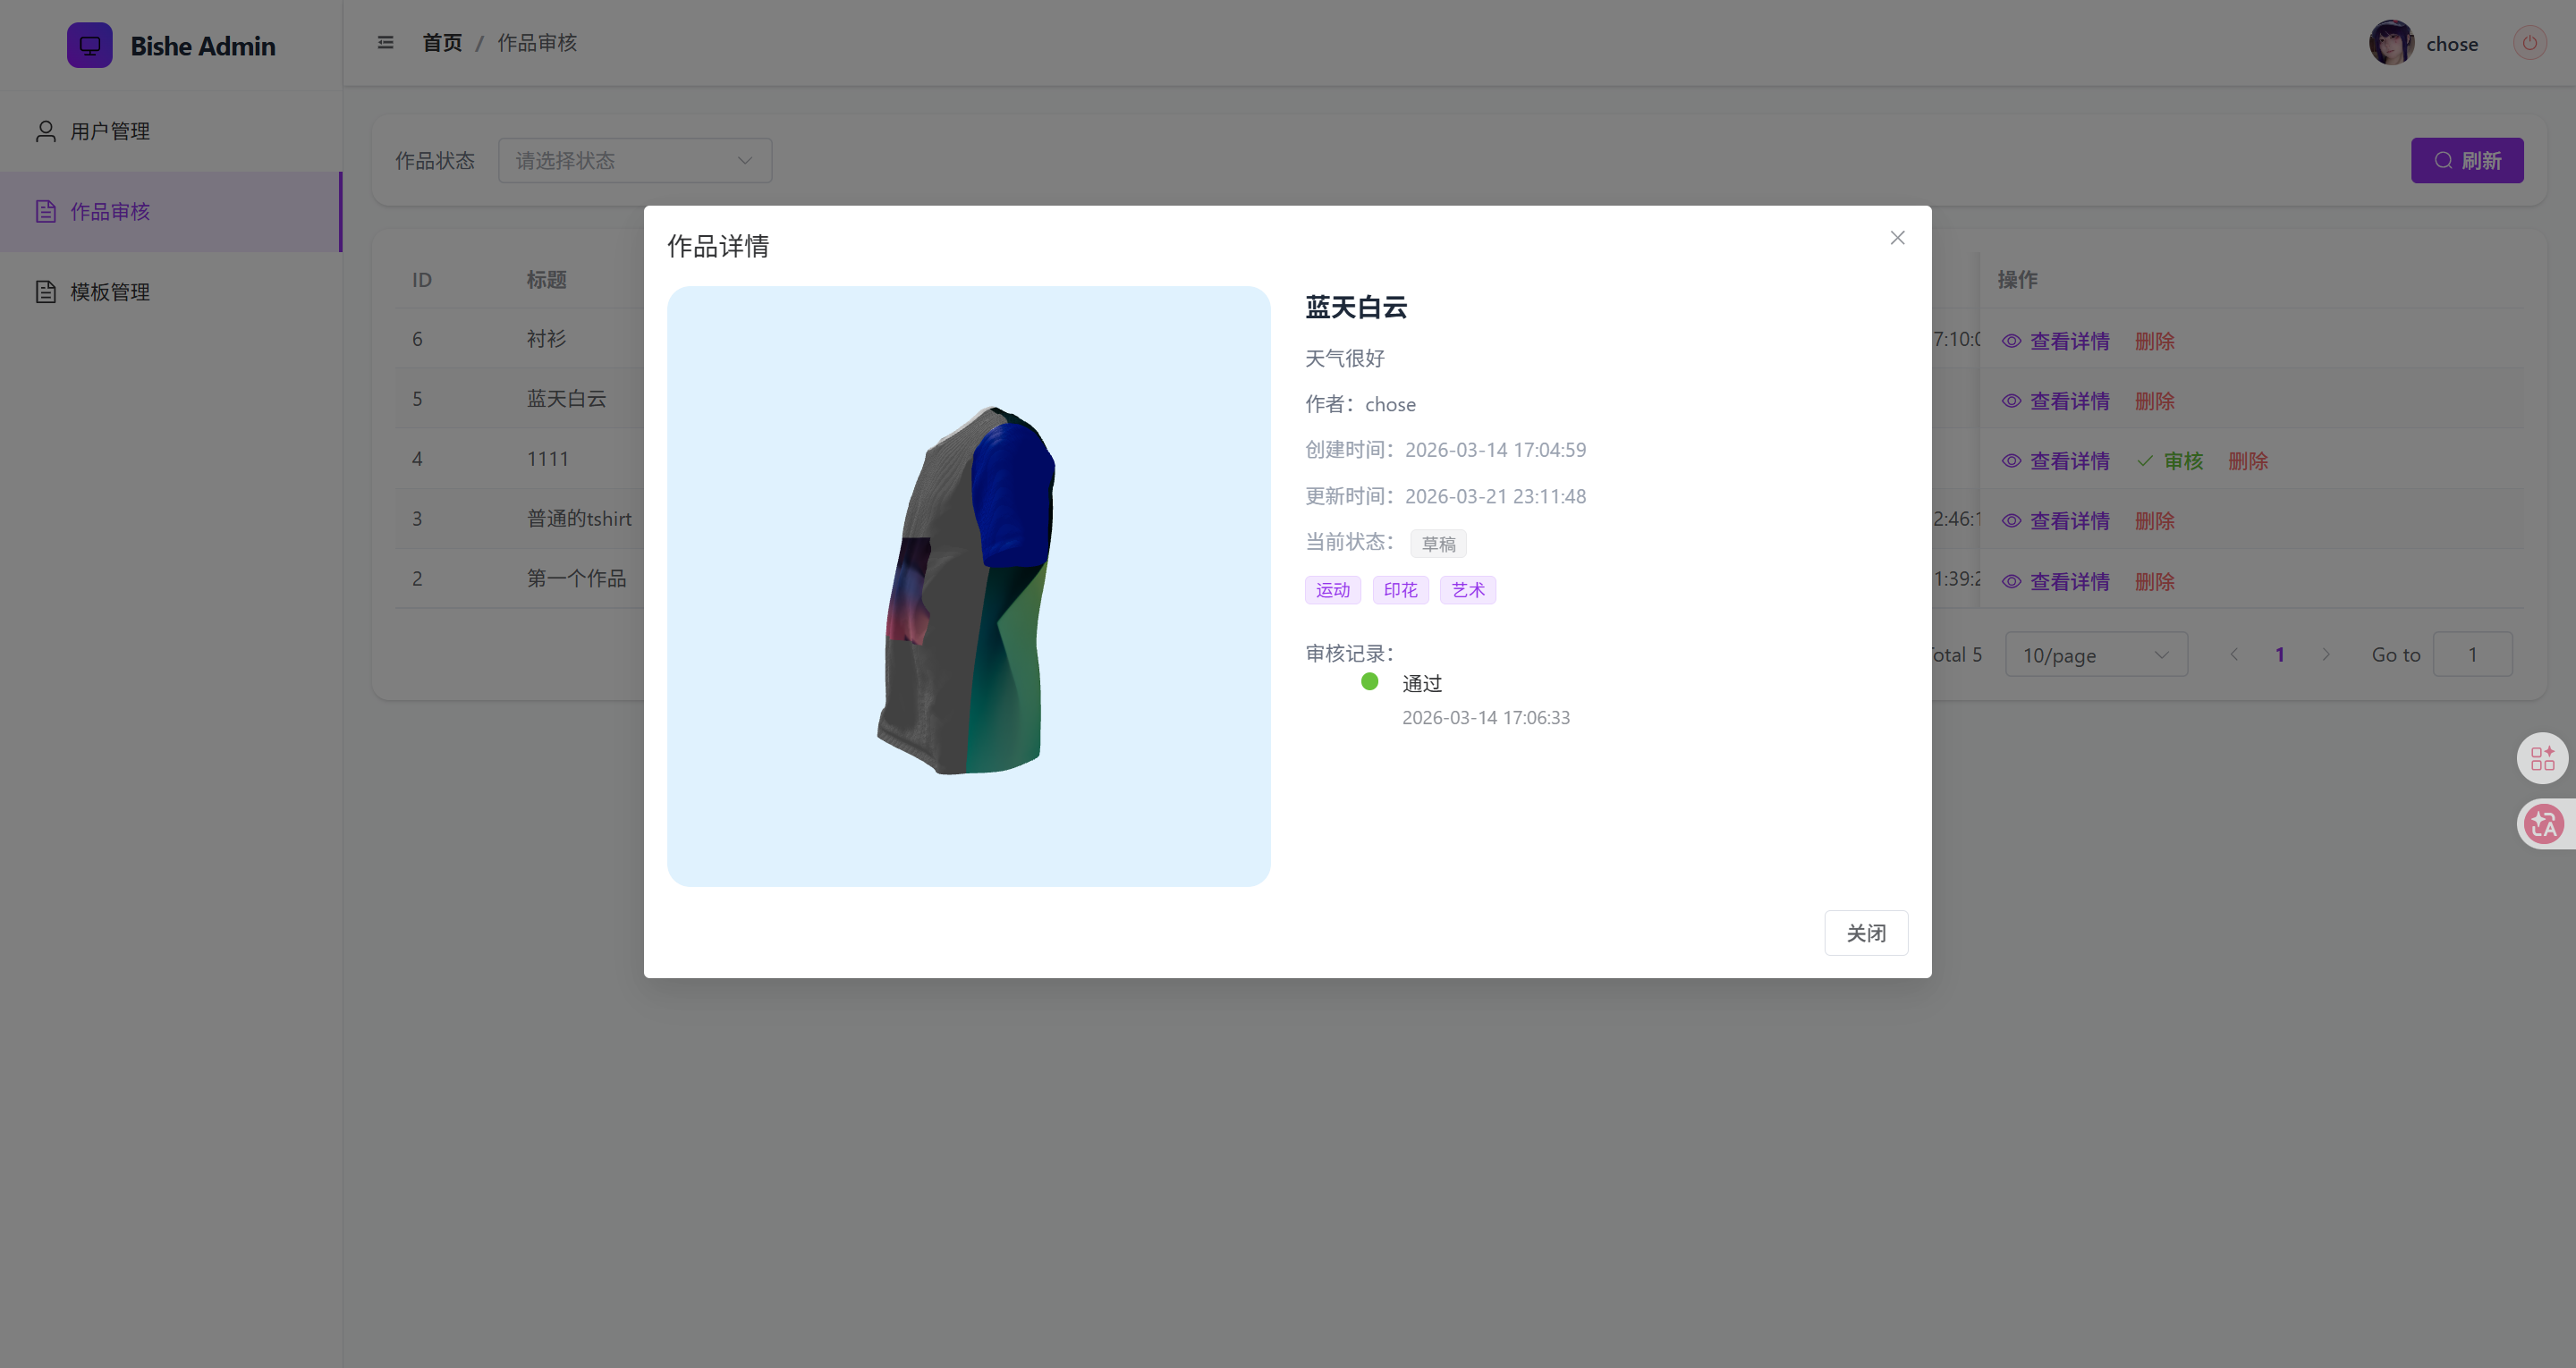
\includegraphics[width=0.85\textwidth]{test22}
	\caption{审核作品展示}
	\label{fig:test-admin-review}
\end{figure}

\subsubsection{模型管理}

测试用例如表~\ref{tab:testcase-admin-model}所示。

\begin{table}[H]
	\centering
	\caption{模型管理测试用例}
	\label{tab:testcase-admin-model}
	\renewcommand{\arraystretch}{1.25}
	\setlength{\tabcolsep}{0.2ex}
	\begin{tabularx}{\textwidth}{@{}>{\raggedright\arraybackslash}p{0.12\textwidth} >{\raggedright\arraybackslash}p{0.22\textwidth} >{\raggedright\arraybackslash}X >{\raggedright\arraybackslash}X@{}}
		\toprule
		\textbf{\mbox{用例ID}} & \textbf{\mbox{前置条件}} & \textbf{\mbox{测试步骤}} & \textbf{\mbox{期望结果}} \\
		\midrule
		\mbox{017} & 已登录后台管理端；具备模型管理权限。 & 1. 查询模型列表；\newline 2. 上传模型信息。 & 1. 模型列表显示上传的模型信息；\newline 2. 上传模型信息成功后，模型列表中可见该模型。 \\
		\bottomrule
	\end{tabularx}
\end{table}

测试结果与期望一致：模型列表查询正常，上传模型成功提示明确，新增条目可在列表中正确显示与查询。结果如图~\ref{fig:test-model-list}和图~\ref{fig:test-model-upload}所示。

\begin{figure}[H]
	\centering
	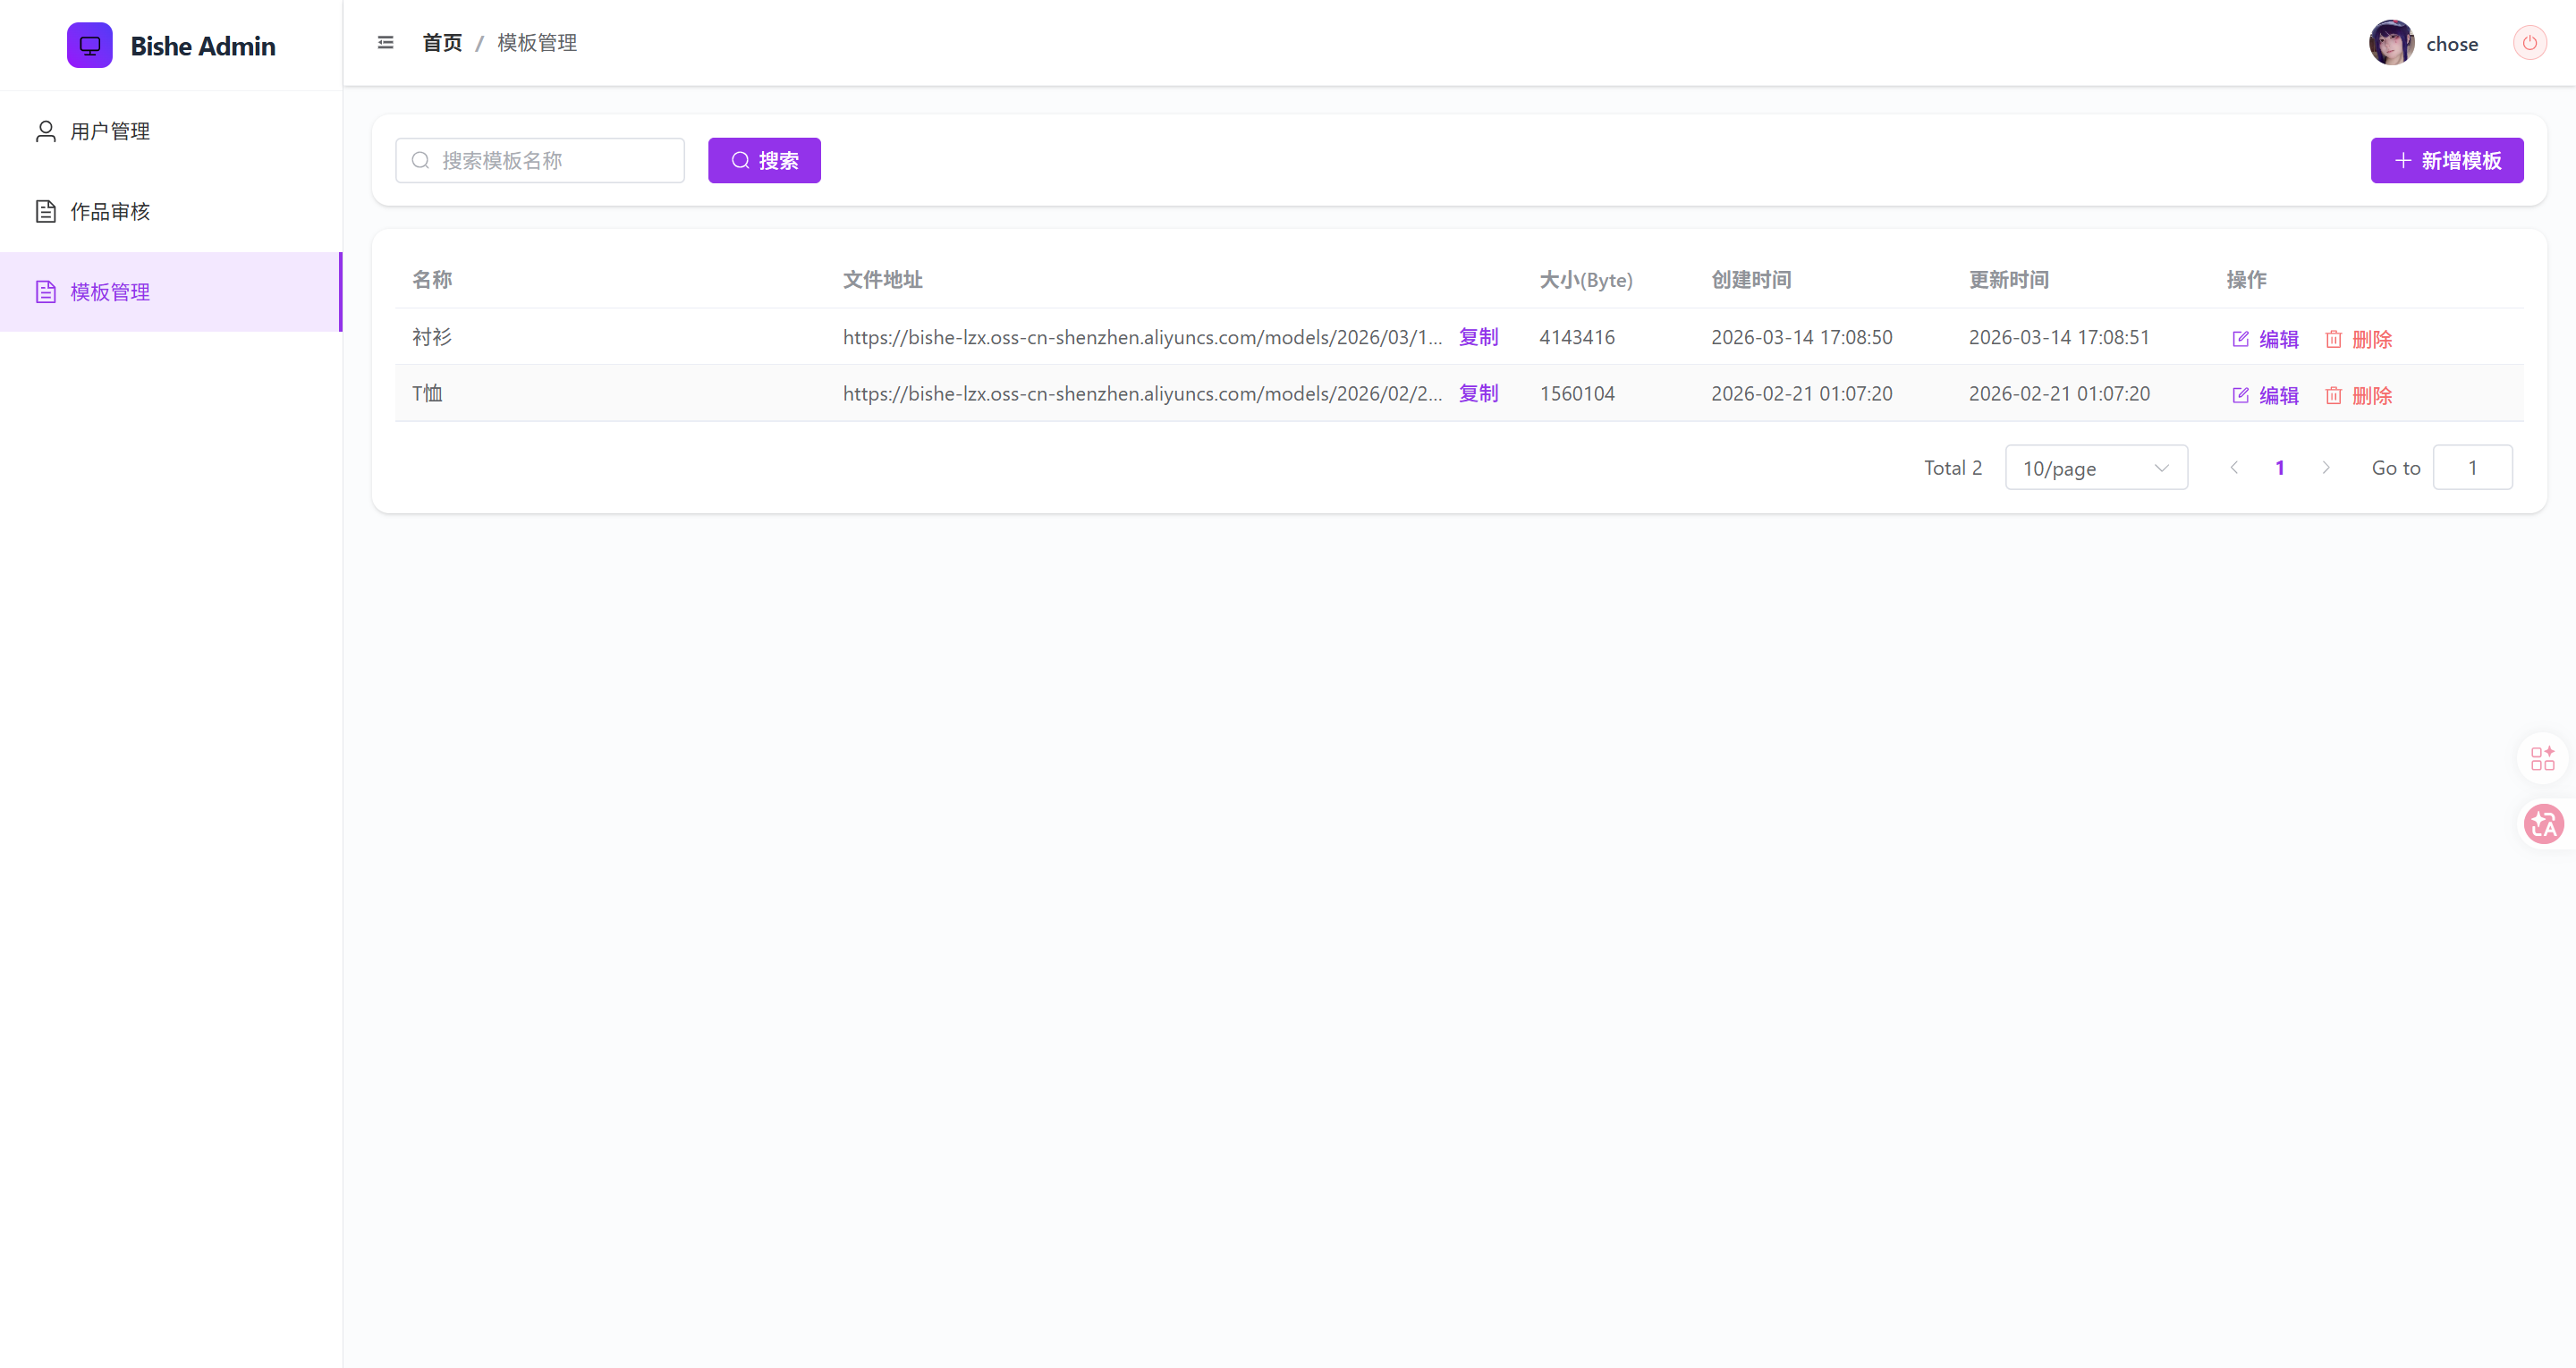
\includegraphics[width=0.85\textwidth]{test23}
	\caption{模型列表展示}
	\label{fig:test-model-list}
\end{figure}

\begin{figure}[H]
	\centering
	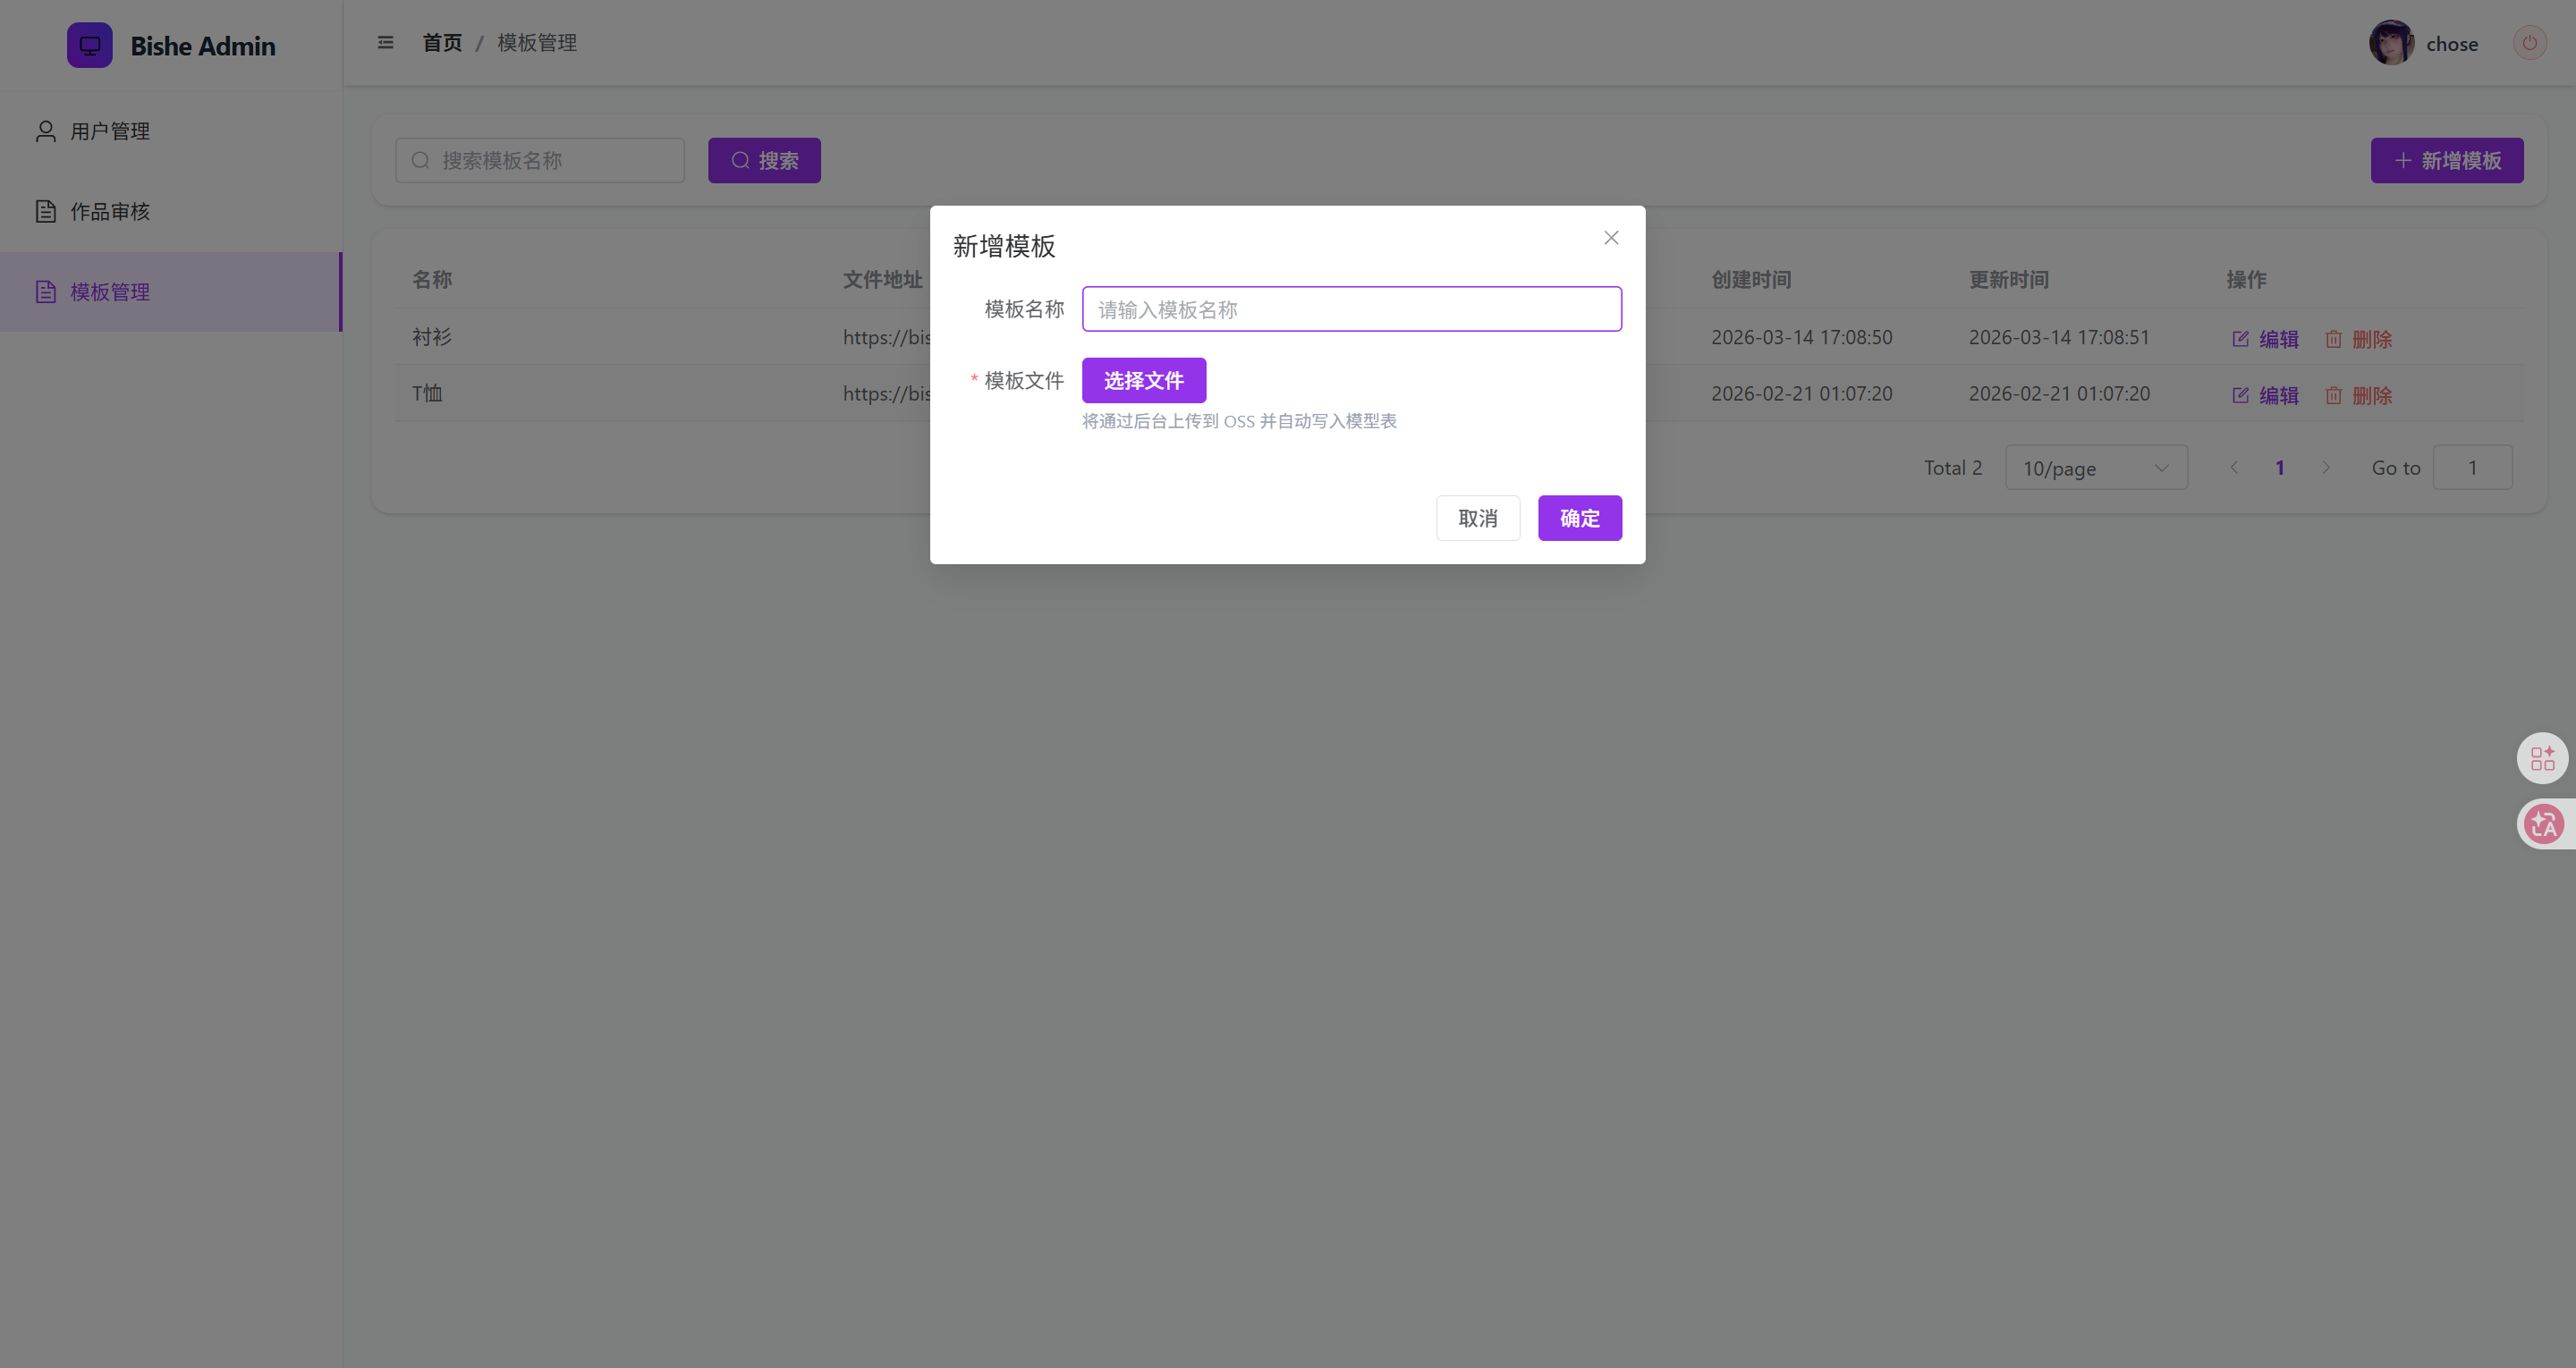
\includegraphics[width=0.85\textwidth]{test24}
	\caption{上传模型展示}
	\label{fig:test-model-upload}
\end{figure}

\chapter{总结与展望}

\section{总结}

本课题围绕“融合 3D 定制与 AI 虚拟试穿的服装创意分享平台”的设计与实现展开研究，面向普通用户提供从创意生成、3D 服装定制、AI 试穿展示到作品发布分享的一体化流程，并配套实现后台管理系统以支撑平台内容治理与资源维护。通过对需求分析、系统设计、核心功能实现与测试验证的完整闭环，平台能够满足用户个性化创作与社区分享的实际需求。

毕业设计的主要工作与成果总结如下：
\begin{enumerate}[label=(\arabic*)]
	\item 完成系统需求分析与总体架构设计。结合平台“创作—展示—传播”的业务特点，对普通用户与管理员两类角色进行功能划分，明确用户模块、3D 服装定制模块、AI 虚拟试穿模块、创意广场模块、作品管理模块与后台管理模块等核心功能，并在此基础上完成系统整体架构与数据流转设计，为后续开发提供清晰边界与实现路径。
	\item 实现 3D 服装定制与可视化交互能力。定制模块支持服装款式选择与属性调整（如颜色、材质、纹理等），并提供旋转、缩放、视角重置等交互操作，使用户能够在设计阶段获得直观、可控的视觉反馈，降低设计门槛并提升创作体验。
	\item 实现 AI 虚拟试穿能力并与作品资产联动。平台支持用户在作品详情中发起试穿任务，展示任务状态与生成结果，提供下载与再次生成等操作；同时将试穿结果纳入作品资产体系，形成“定制—试穿—发布”的闭环链路，提升作品表达的真实感与传播价值。
	\item 实现创意广场与作品管理功能，形成内容发布与互动体系。创意广场提供作品浏览、搜索筛选与互动能力（点赞、收藏、关注等），作品管理模块支持作品创建、编辑、提审、发布/下架等状态流转，保证内容发布流程可控并支持社区侧展示与传播。
	\item 实现后台管理系统，支撑资源与内容治理。后台管理模块提供管理员登录与权限控制，支持用户管理、作品审核与模型管理等操作，实现对平台内容与资源的统一维护，为平台运行提供基础保障。
\end{enumerate}

\section{展望}

尽管平台已实现论文目标并能够稳定完成主要业务流程，但在模型资源丰富度、试穿效果质量、性能与工程化能力等方面仍有提升空间，后续可从以下方向进一步完善。
\begin{enumerate}[label=(\arabic*)]
	\item 提升 3D 定制能力与资源体系。扩充服装模型与面料材质库，支持更多服装品类与部件组合；引入更细粒度的参数化版型与布料物理模拟，提高定制的真实性与可玩性；在移动端与低性能设备上进一步优化渲染资源加载与交互性能。
	\item 提升 AI 试穿效果与稳定性。进一步优化人像预处理与服装约束策略，提升对不同姿态、光照、遮挡场景的鲁棒性；引入更精细的控制条件（如人体关键点、分割掩码、深度信息等）提升服装贴合与纹理一致性；完善任务队列与失败重试机制，提升生成链路在高并发场景下的稳定性。
	\item 完善内容生态与个性化推荐。结合用户兴趣与互动行为构建推荐策略，提升创意广场内容分发效率；增加作品标签体系与主题活动机制，促进优质内容沉淀；完善评论审核与举报流程，提升社区治理能力。
	\item 强化安全与工程化能力。进一步细化权限模型与接口访问控制，完善日志审计与异常监控；在部署层面引入更标准化的 CI/CD、自动化回归测试与性能压测流程；针对关键接口与资源加载链路进行缓存与限流优化，提升系统可用性与可维护性。
\end{enumerate}

\bibliography{bibHzu}

\chapterspecialcenter{致 谢}

大学的时光一眨眼就过去了，回想起四年的点点滴滴却又是那么漫长，充实。这一路上，我遇到了很多朋友，以及照料我的老师们，感谢他们的支持与指导，才能让我走到今天，真的不甚感激。即将离开校园，也意味着我们不再是学生了，也要成为大家口中的牛马了，但是这路上的经历我都会牢牢记住，哪天累了回想起来，也会会心一笑。唉，真是携来百侣曾游，忆往昔峥嵘岁月稠啊。最后，再次感谢我的老师，朋友们，谢谢你们！

\chapterspecialcenter{附 录}

本附录 A 到附录 F 主要说明 5.2 系统功能模块实现的关键源码，包括用户管理、3D 服装定制、AI 虚拟试穿、创意广场、作品管理、后台管理的关键代码。

\clearpage
\noindent\textbf{附录 A \quad 用户管理模块}

\noindent\textbf{后端代码}
\begin{verbatim}
package model

import (
	"database/sql"
	"fmt"
	"strings"
	"time"

	"github.com/chosetop/bishe_back/internal/config"
)

type User struct {
	ID        int       `json:"id"`
	Username  string    `json:"username"`
	Password  string    `json:"-"`
	Avatar    string    `json:"avatar"`
	Role      int       `json:"role"`
	CreatedAt time.Time `json:"created_at"`
	UpdatedAt time.Time `json:"updated_at"`
}

func CreateUser(username, passwordHash string) error {
	stmt, err := config.DB.Prepare("INSERT INTO users(username, password) VALUES(?, ?)")
	if err != nil {
		return err
	}
	defer stmt.Close()
	_, err = stmt.Exec(username, passwordHash)
	return err
}

func GetUserByUsername(username string) (*User, error) {
	row := config.DB.QueryRow("SELECT id, username, password, COALESCE(avatar, ''), role, created_at, updated_at FROM users WHERE username = ?", username)
	var user User
	err := row.Scan(&user.ID, &user.Username, &user.Password, &user.Avatar, &user.Role, &user.CreatedAt, &user.UpdatedAt)
	if err != nil {
		if err == sql.ErrNoRows {
			return nil, nil
		}
		return nil, err
	}
	return &user, nil
}

func UpdateUserFields(id int, username *string, avatar *string, role *int) (int64, error) {
	fields := make([]string, 0, 3)
	args := make([]any, 0, 3)
	if username != nil {
		fields = append(fields, "username = ?")
		args = append(args, *username)
	}
	if avatar != nil {
		fields = append(fields, "avatar = ?")
		args = append(args, *avatar)
	}
	if role != nil {
		fields = append(fields, "role = ?")
		args = append(args, *role)
	}
	if len(fields) == 0 {
		return 0, nil
	}
	args = append(args, id)
	query := fmt.Sprintf("UPDATE users SET %s WHERE id = ?", strings.Join(fields, ", "))
	res, err := config.DB.Exec(query, args...)
	if err != nil {
		return 0, err
	}
	return res.RowsAffected()
}

func DeleteUser(id int) (int64, error) {
	res, err := config.DB.Exec("DELETE FROM users WHERE id = ?", id)
	if err != nil {
		return 0, err
	}
	return res.RowsAffected()
}
\end{verbatim}
\iffalse
package model

import (
	"database/sql"
	"fmt"
	"strings"
	"time"

	"github.com/chosetop/bishe_back/internal/config"
)

type User struct {
	ID        int       `json:"id"`
	Username  string    `json:"username"`
	Password  string    `json:"-"` // 不返回密码
	Avatar    string    `json:"avatar"`
	Role      int       `json:"role"`
	CreatedAt time.Time `json:"created_at"`
	UpdatedAt time.Time `json:"updated_at"`
}

// CreateUser 创建用户
func CreateUser(username, passwordHash string) error {
	stmt, err := config.DB.Prepare("INSERT INTO users(username, password) VALUES(?, ?)")
	if err != nil {
		return err
	}
	defer stmt.Close()

	_, err = stmt.Exec(username, passwordHash)
	return err
}

// GetUserByUsername 根据用户名获取用户
func GetUserByUsername(username string) (*User, error) {
	row := config.DB.QueryRow("SELECT id, username, password, COALESCE(avatar, ''), role, created_at, updated_at FROM users WHERE username = ?", username)

	var user User
	err := row.Scan(&user.ID, &user.Username, &user.Password, &user.Avatar, &user.Role, &user.CreatedAt, &user.UpdatedAt)
	if err != nil {
		if err == sql.ErrNoRows {
			return nil, nil // 用户不存在
		}
		return nil, err
	}
	return &user, nil
}

// GetUserByID 根据ID获取用户
func GetUserByID(id int) (*User, error) {
	row := config.DB.QueryRow("SELECT id, username, COALESCE(avatar, ''), role, created_at, updated_at FROM users WHERE id = ?", id)

	var user User
	err := row.Scan(&user.ID, &user.Username, &user.Avatar, &user.Role, &user.CreatedAt, &user.UpdatedAt)
	if err != nil {
		if err == sql.ErrNoRows {
			return nil, nil
		}
		return nil, err
	}
	return &user, nil
}

func CountUsers(username string) (int, error) {
	var (
		where string
		args  []any
	)
	if username != "" {
		where = " WHERE username LIKE ?"
		args = append(args, "%"+username+"%")
	}

	row := config.DB.QueryRow("SELECT COUNT(1) FROM users"+where, args...)
	var total int
	if err := row.Scan(&total); err != nil {
		return 0, err
	}
	return total, nil
}

func ListUsers(username string, limit, offset int) ([]User, error) {
	var (
		where string
		args  []any
	)
	if username != "" {
		where = " WHERE username LIKE ?"
		args = append(args, "%"+username+"%")
	}
	args = append(args, limit, offset)

	rows, err := config.DB.Query(
		"SELECT id, username, COALESCE(avatar, ''), role, created_at, updated_at FROM users"+where+" ORDER BY id DESC LIMIT ? OFFSET ?",
		args...,
	)
	if err != nil {
		return nil, err
	}
	defer rows.Close()

	list := make([]User, 0, limit)
	for rows.Next() {
		var u User
		if err := rows.Scan(&u.ID, &u.Username, &u.Avatar, &u.Role, &u.CreatedAt, &u.UpdatedAt); err != nil {
			return nil, err
		}
		list = append(list, u)
	}
	if err := rows.Err(); err != nil {
		return nil, err
	}
	return list, nil
}

func GetUserAuthByID(id int) (*User, error) {
	row := config.DB.QueryRow("SELECT id, username, password, COALESCE(avatar, ''), role, created_at, updated_at FROM users WHERE id = ?", id)

	var user User
	err := row.Scan(&user.ID, &user.Username, &user.Password, &user.Avatar, &user.Role, &user.CreatedAt, &user.UpdatedAt)
	if err != nil {
		if err == sql.ErrNoRows {
			return nil, nil
		}
		return nil, err
	}
	return &user, nil
}

func UpdateUserFields(id int, username *string, avatar *string, role *int) (int64, error) {
	fields := make([]string, 0, 3)
	args := make([]any, 0, 3)

	if username != nil {
		fields = append(fields, "username = ?")
		args = append(args, *username)
	}
	if avatar != nil {
		fields = append(fields, "avatar = ?")
		args = append(args, *avatar)
	}
	if role != nil {
		fields = append(fields, "role = ?")
		args = append(args, *role)
	}
	if len(fields) == 0 {
		return 0, nil
	}

	args = append(args, id)
	query := fmt.Sprintf("UPDATE users SET %s WHERE id = ?", strings.Join(fields, ", "))
	res, err := config.DB.Exec(query, args...)
	if err != nil {
		return 0, err
	}
	return res.RowsAffected()
}

func UpdateUserPassword(id int, passwordHash string) (int64, error) {
	res, err := config.DB.Exec("UPDATE users SET password = ? WHERE id = ?", passwordHash, id)
	if err != nil {
		return 0, err
	}
	return res.RowsAffected()
}

func DeleteUser(id int) (int64, error) {
	res, err := config.DB.Exec("DELETE FROM users WHERE id = ?", id)
	if err != nil {
		return 0, err
	}
	return res.RowsAffected()
}

\end{verbatim}
\fi

\clearpage
\noindent\textbf{附录 B \quad 3D 服装定制模块}

\noindent\textbf{后端代码}
\begin{verbatim}
package front

import (
	"encoding/json"
	"net/http"
	"strconv"
	"time"

	"github.com/chosetop/bishe_back/internal/model"
	"github.com/gin-gonic/gin"
)

type CreateWorkInput struct {
	Title       string          `json:"title" binding:"required"`
	Description string          `json:"description"`
	CoverFileID *int64          `json:"cover_file_id"`
	ParamsJSON  json.RawMessage `json:"params_json" binding:"required"`
	ModelFileID *int64          `json:"model_file_id"`
	Tags        []string        `json:"tags"`
}

type UpdateWorkInput struct {
	Title       *string         `json:"title"`
	Description *string         `json:"description"`
	CoverFileID *int64          `json:"cover_file_id"`
	ParamsJSON  json.RawMessage `json:"params_json"`
	ModelFileID *int64          `json:"model_file_id"`
	Tags        []string        `json:"tags"`
}

func CreateWork(c *gin.Context) {
	userIDVal, ok := c.Get("userID")
	if !ok {
		c.JSON(http.StatusUnauthorized, gin.H{"success": false, "message": "未登录"})
		return
	}
	userID, ok := userIDVal.(int)
	if !ok || userID <= 0 {
		c.JSON(http.StatusUnauthorized, gin.H{"success": false, "message": "未登录"})
		return
	}

	var input CreateWorkInput
	if err := c.ShouldBindJSON(&input); err != nil {
		c.JSON(http.StatusOK, gin.H{"success": false, "message": err.Error()})
		return
	}
	if len(input.ParamsJSON) == 0 {
		c.JSON(http.StatusBadRequest, gin.H{"success": false, "message": "params_json不能为空"})
		return
	}

	workID, err := model.CreateDesignWork(int64(userID), input.Title, input.Description, input.CoverFileID)
	if err != nil {
		c.JSON(http.StatusInternalServerError, gin.H{"success": false, "error": "创建作品失败"})
		return
	}

	versionID, err := model.CreateDesignVersion(workID, 1, input.ParamsJSON, input.ModelFileID)
	if err != nil {
		c.JSON(http.StatusInternalServerError, gin.H{"success": false, "error": "创建版本失败"})
		return
	}
	_, _ = model.UpdateDesignWorkFields(workID, nil, nil, nil, nil, &versionID, nil)

	if input.Tags != nil {
		_ = model.SetWorkTags(workID, input.Tags)
	}

	work, _ := model.GetDesignWorkByID(workID)
	version, _ := model.GetDesignVersionByID(versionID)
	c.JSON(http.StatusOK, gin.H{"success": true, "work": work, "version": version})
}

func UpdateWork(c *gin.Context) {
	userIDVal, ok := c.Get("userID")
	if !ok {
		c.JSON(http.StatusUnauthorized, gin.H{"success": false, "message": "未登录"})
		return
	}
	userID, ok := userIDVal.(int)
	if !ok || userID <= 0 {
		c.JSON(http.StatusUnauthorized, gin.H{"success": false, "message": "未登录"})
		return
	}

	workID, err := strconv.ParseInt(c.Param("id"), 10, 64)
	if err != nil || workID <= 0 {
		c.JSON(http.StatusBadRequest, gin.H{"success": false, "message": "ID不合法"})
		return
	}

	work, err := model.GetDesignWorkByID(workID)
	if err != nil {
		c.JSON(http.StatusInternalServerError, gin.H{"success": false, "error": "获取作品失败"})
		return
	}
	if work == nil || work.UserID != int64(userID) {
		c.JSON(http.StatusOK, gin.H{"success": false, "message": "作品不存在"})
		return
	}

	var input UpdateWorkInput
	if err := c.ShouldBindJSON(&input); err != nil {
		c.JSON(http.StatusOK, gin.H{"success": false, "message": err.Error()})
		return
	}

	_, err = model.UpdateDesignWorkFields(workID, input.Title, input.Description, input.CoverFileID, nil, nil, nil)
	if err != nil {
		c.JSON(http.StatusInternalServerError, gin.H{"success": false, "error": "更新作品失败"})
		return
	}
	if work.CurrentVersionID != nil {
		_, _ = model.UpdateDesignVersionFields(*work.CurrentVersionID, input.ParamsJSON, input.ModelFileID, true)
	}
	if input.Tags != nil {
		_ = model.SetWorkTags(workID, input.Tags)
	}

	work, _ = model.GetDesignWorkByID(workID)
	var version *model.DesignVersion
	if work != nil && work.CurrentVersionID != nil {
		version, _ = model.GetDesignVersionByID(*work.CurrentVersionID)
	}
	c.JSON(http.StatusOK, gin.H{"success": true, "work": work, "version": version})
}

func SubmitWork(c *gin.Context) {
	userIDVal, ok := c.Get("userID")
	if !ok {
		c.JSON(http.StatusUnauthorized, gin.H{"success": false, "message": "未登录"})
		return
	}
	userID, ok := userIDVal.(int)
	if !ok || userID <= 0 {
		c.JSON(http.StatusUnauthorized, gin.H{"success": false, "message": "未登录"})
		return
	}

	workID, err := strconv.ParseInt(c.Param("id"), 10, 64)
	if err != nil || workID <= 0 {
		c.JSON(http.StatusBadRequest, gin.H{"success": false, "message": "ID不合法"})
		return
	}
	work, err := model.GetDesignWorkByID(workID)
	if err != nil {
		c.JSON(http.StatusInternalServerError, gin.H{"success": false, "error": "获取作品失败"})
		return
	}
	if work == nil || work.UserID != int64(userID) || work.CurrentVersionID == nil {
		c.JSON(http.StatusOK, gin.H{"success": false, "message": "作品不存在"})
		return
	}

	status := model.DesignStatusSubmitted
	now := time.Now()
	_, _ = model.UpdateDesignWorkFields(workID, nil, nil, nil, &status, nil, nil)
	_, _ = model.UpdateDesignVersionSubmittedAt(*work.CurrentVersionID, now)

	work, _ = model.GetDesignWorkByID(workID)
	version, _ := model.GetDesignVersionByID(*work.CurrentVersionID)
	c.JSON(http.StatusOK, gin.H{"success": true, "work": work, "version": version})
}
\end{verbatim}
\iffalse
package front

import (
	"context"
	"crypto/rand"
	"encoding/hex"
	"encoding/json"
	"fmt"
	"net/http"
	"os"
	"strconv"
	"time"

	"github.com/chosetop/bishe_back/internal/config"
	"github.com/chosetop/bishe_back/internal/model"
	"github.com/gin-gonic/gin"
)

const tryOnQueueKey = "queue:tryon:tasks"

type CreateWorkInput struct {
	Title       string          `json:"title" binding:"required"`
	Description string          `json:"description"`
	CoverFileID *int64          `json:"cover_file_id"`
	ParamsJSON  json.RawMessage `json:"params_json" binding:"required"`
	ModelFileID *int64          `json:"model_file_id"`
	Tags        []string        `json:"tags"`
}

func CreateWork(c *gin.Context) {
	userIDVal, ok := c.Get("userID")
	if !ok {
		c.JSON(http.StatusUnauthorized, gin.H{"success": false, "message": "未登录"})
		return
	}
	userID, ok := userIDVal.(int)
	if !ok || userID <= 0 {
		c.JSON(http.StatusUnauthorized, gin.H{"success": false, "message": "未登录"})
		return
	}

	var input CreateWorkInput
	if err := c.ShouldBindJSON(&input); err != nil {
		c.JSON(http.StatusOK, gin.H{"success": false, "message": err.Error()})
		return
	}
	if len(input.ParamsJSON) == 0 {
		c.JSON(http.StatusBadRequest, gin.H{"success": false, "message": "params_json不能为空"})
		return
	}

	workID, err := model.CreateDesignWork(int64(userID), input.Title, input.Description, input.CoverFileID)
	if err != nil {
		c.JSON(http.StatusInternalServerError, gin.H{"success": false, "error": "创建作品失败"})
		return
	}

	versionID, err := model.CreateDesignVersion(workID, 1, input.ParamsJSON, input.ModelFileID)
	if err != nil {
		c.JSON(http.StatusInternalServerError, gin.H{"success": false, "error": "创建版本失败"})
		return
	}

	_, err = model.UpdateDesignWorkFields(workID, nil, nil, nil, nil, &versionID, nil)
	if err != nil {
		c.JSON(http.StatusInternalServerError, gin.H{"success": false, "error": "更新作品失败"})
		return
	}

	if len(input.Tags) > 0 {
		model.SetWorkTags(workID, input.Tags)
	}

	work, _ := model.GetDesignWorkByID(workID)
	version, _ := model.GetDesignVersionByID(versionID)
	c.JSON(http.StatusOK, gin.H{"success": true, "work": work, "version": version})
}

type UpdateWorkInput struct {
	Title       *string         `json:"title"`
	Description *string         `json:"description"`
	CoverFileID *int64          `json:"cover_file_id"`
	ParamsJSON  json.RawMessage `json:"params_json"`
	ModelFileID *int64          `json:"model_file_id"`
	Tags        []string        `json:"tags"`
}

type CreateTryOnTaskInput struct {
	BodyType   string          `json:"body_type" binding:"required"`
	SceneStyle string          `json:"scene_style" binding:"required"`
	InputRefs  json.RawMessage `json:"input_refs"`
}

func UpdateWork(c *gin.Context) {
	userIDVal, ok := c.Get("userID")
	if !ok {
		c.JSON(http.StatusUnauthorized, gin.H{"success": false, "message": "未登录"})
		return
	}
	userID, ok := userIDVal.(int)
	if !ok || userID <= 0 {
		c.JSON(http.StatusUnauthorized, gin.H{"success": false, "message": "未登录"})
		return
	}

	workID, err := strconv.ParseInt(c.Param("id"), 10, 64)
	if err != nil || workID <= 0 {
		c.JSON(http.StatusBadRequest, gin.H{"success": false, "message": "ID不合法"})
		return
	}

	work, err := model.GetDesignWorkByID(workID)
	if err != nil {
		c.JSON(http.StatusInternalServerError, gin.H{"success": false, "error": "获取作品失败"})
		return
	}
	if work == nil || work.UserID != int64(userID) {
		c.JSON(http.StatusOK, gin.H{"success": false, "message": "作品不存在"})
		return
	}
	if work.Status == model.DesignStatusSubmitted || work.Status == model.DesignStatusApproved || work.Status == model.DesignStatusPublished {
		c.JSON(http.StatusOK, gin.H{"success": false, "message": "当前状态不可编辑"})
		return
	}

	var input UpdateWorkInput
	if err := c.ShouldBindJSON(&input); err != nil {
		c.JSON(http.StatusOK, gin.H{"success": false, "message": err.Error()})
		return
	}

	var status *int
	if work.Status == model.DesignStatusRejected {
		s := model.DesignStatusDraft
		status = &s
	}

	_, err = model.UpdateDesignWorkFields(workID, input.Title, input.Description, input.CoverFileID, status, nil, nil)
	if err != nil {
		c.JSON(http.StatusInternalServerError, gin.H{"success": false, "error": "更新作品失败"})
		return
	}

	var versionID int64
	if work.CurrentVersionID != nil {
		versionID = *work.CurrentVersionID
	} else {
		latest, err := model.GetLatestDesignVersionByWorkID(workID)
		if err != nil || latest == nil {
			c.JSON(http.StatusInternalServerError, gin.H{"success": false, "error": "获取版本失败"})
			return
		}
		versionID = latest.ID
		_, _ = model.UpdateDesignWorkFields(workID, nil, nil, nil, nil, &versionID, nil)
	}

	clearSubmittedAt := work.Status == model.DesignStatusRejected || len(input.ParamsJSON) > 0 || input.ModelFileID != nil
	if clearSubmittedAt {
		_, err = model.UpdateDesignVersionFields(versionID, input.ParamsJSON, input.ModelFileID, true)
		if err != nil {
			c.JSON(http.StatusInternalServerError, gin.H{"success": false, "error": "更新版本失败"})
			return
		}
	}

	work, _ = model.GetDesignWorkByID(workID)
	var version *model.DesignVersion
	if work != nil && work.CurrentVersionID != nil {
		version, _ = model.GetDesignVersionByID(*work.CurrentVersionID)
	}

	if input.Tags != nil {
		model.SetWorkTags(workID, input.Tags)
	}

	c.JSON(http.StatusOK, gin.H{"success": true, "work": work, "version": version})
}

func SubmitWork(c *gin.Context) {
	userIDVal, ok := c.Get("userID")
	if !ok {
		c.JSON(http.StatusUnauthorized, gin.H{"success": false, "message": "未登录"})
		return
	}
	userID, ok := userIDVal.(int)
	if !ok || userID <= 0 {
		c.JSON(http.StatusUnauthorized, gin.H{"success": false, "message": "未登录"})
		return
	}

	workID, err := strconv.ParseInt(c.Param("id"), 10, 64)
	if err != nil || workID <= 0 {
		c.JSON(http.StatusBadRequest, gin.H{"success": false, "message": "ID不合法"})
		return
	}

	work, err := model.GetDesignWorkByID(workID)
	if err != nil {
		c.JSON(http.StatusInternalServerError, gin.H{"success": false, "error": "获取作品失败"})
		return
	}
	if work == nil || work.UserID != int64(userID) {
		c.JSON(http.StatusOK, gin.H{"success": false, "message": "作品不存在"})
		return
	}
	if work.Status != model.DesignStatusDraft && work.Status != model.DesignStatusRejected {
		c.JSON(http.StatusOK, gin.H{"success": false, "message": "当前状态不可提交"})
		return
	}
	if work.CurrentVersionID == nil {
		c.JSON(http.StatusOK, gin.H{"success": false, "message": "缺少版本信息"})
		return
	}

	status := model.DesignStatusSubmitted
	now := time.Now()
	_, err = model.UpdateDesignWorkFields(workID, nil, nil, nil, &status, nil, nil)
	if err != nil {
		c.JSON(http.StatusInternalServerError, gin.H{"success": false, "error": "提交失败"})
		return
	}
	_, err = model.UpdateDesignVersionSubmittedAt(*work.CurrentVersionID, now)
	if err != nil {
		c.JSON(http.StatusInternalServerError, gin.H{"success": false, "error": "提交失败"})
		return
	}

	work, _ = model.GetDesignWorkByID(workID)
	version, _ := model.GetDesignVersionByID(*work.CurrentVersionID)
	c.JSON(http.StatusOK, gin.H{"success": true, "work": work, "version": version})
}

func ListWorks(c *gin.Context) {
	userIDVal, ok := c.Get("userID")
	if !ok {
		c.JSON(http.StatusUnauthorized, gin.H{"success": false, "message": "未登录"})
		return
	}
	userID, ok := userIDVal.(int)
	if !ok || userID <= 0 {
		c.JSON(http.StatusUnauthorized, gin.H{"success": false, "message": "未登录"})
		return
	}

	page, _ := strconv.Atoi(c.DefaultQuery("page", "1"))
	pageSize, _ := strconv.Atoi(c.DefaultQuery("page_size", "20"))
	if page <= 0 {
		page = 1
	}
	if pageSize <= 0 {
		pageSize = 20
	}
	if pageSize > 100 {
		pageSize = 100
	}
	offset := (page - 1) * pageSize

	var status *int
	if s := c.Query("status"); s != "" {
		if v, err := strconv.Atoi(s); err == nil && v > 0 {
			status = &v
		}
	}
	uid := int64(userID)
	total, err := model.CountDesignWorks(&uid, status)
	if err != nil {
		c.JSON(http.StatusInternalServerError, gin.H{"success": false, "error": "获取作品失败"})
		return
	}
	list, err := model.ListDesignWorks(&uid, status, pageSize, offset)
	if err != nil {
		c.JSON(http.StatusInternalServerError, gin.H{"success": false, "error": "获取作品失败"})
		return
	}

	type WorkListItem struct {
		Work    model.DesignWork     `json:"work"`
		Version *model.DesignVersion `json:"version"`
		Model   *model.ModelFile     `json:"model"`
	}
	items := make([]WorkListItem, 0, len(list))
	for _, w := range list {
		var version *model.DesignVersion
		var modelFile *model.ModelFile
		if w.CurrentVersionID != nil {
			version, _ = model.GetDesignVersionByID(*w.CurrentVersionID)
		} else {
			version, _ = model.GetLatestDesignVersionByWorkID(w.ID)
		}
		if version != nil && version.ModelFileID != nil {
			if m, err := model.GetModelFileByID(int(*version.ModelFileID)); err == nil {
				modelFile = m
			}
		}
		items = append(items, WorkListItem{
			Work:    w,
			Version: version,
			Model:   modelFile,
		})
	}

	c.JSON(http.StatusOK, gin.H{
		"success": true,
		"data": gin.H{
			"list":      items,
			"total":     total,
			"page":      page,
			"page_size": pageSize,
		},
	})
}

func GetWork(c *gin.Context) {
	userIDVal, ok := c.Get("userID")
	if !ok {
		c.JSON(http.StatusUnauthorized, gin.H{"success": false, "message": "未登录"})
		return
	}
	userID, ok := userIDVal.(int)
	if !ok || userID <= 0 {
		c.JSON(http.StatusUnauthorized, gin.H{"success": false, "message": "未登录"})
		return
	}

	workID, err := strconv.ParseInt(c.Param("id"), 10, 64)
	if err != nil || workID <= 0 {
		c.JSON(http.StatusBadRequest, gin.H{"success": false, "message": "ID不合法"})
		return
	}

	work, err := model.GetDesignWorkByID(workID)
	if err != nil {
		c.JSON(http.StatusInternalServerError, gin.H{"success": false, "error": "获取作品失败"})
		return
	}
	if work == nil || work.UserID != int64(userID) {
		c.JSON(http.StatusOK, gin.H{"success": false, "message": "作品不存在"})
		return
	}

	var version *model.DesignVersion
	if work.CurrentVersionID != nil {
		version, _ = model.GetDesignVersionByID(*work.CurrentVersionID)
	}
	reviews, _ := model.ListDesignReviewsByWorkID(workID)
	tryOnHistory, _ := model.ListTryOnTasksByWorkID(workID, 10)
	var latestTask *model.TryOnTask
	if len(tryOnHistory) > 0 {
		latestTask = &tryOnHistory[0]
	}

	c.JSON(http.StatusOK, gin.H{
		"success": true,
		"work":    work,
		"version": version,
		"reviews": reviews,
		"tryon": gin.H{
			"latest_task":   latestTask,
			"history_tasks": tryOnHistory,
		},
	})
}

func CreateTryOnTask(c *gin.Context) {
	userIDVal, ok := c.Get("userID")
	if !ok {
		c.JSON(http.StatusUnauthorized, gin.H{"success": false, "message": "未登录"})
		return
	}
	userID, ok := userIDVal.(int)
	if !ok || userID <= 0 {
		c.JSON(http.StatusUnauthorized, gin.H{"success": false, "message": "未登录"})
		return
	}

	workID, err := strconv.ParseInt(c.Param("id"), 10, 64)
	if err != nil || workID <= 0 {
		c.JSON(http.StatusBadRequest, gin.H{"success": false, "message": "ID不合法"})
		return
	}

	work, err := model.GetDesignWorkByID(workID)
	if err != nil {
		c.JSON(http.StatusInternalServerError, gin.H{"success": false, "error": "获取作品失败"})
		return
	}
	if work == nil || work.UserID != int64(userID) {
		c.JSON(http.StatusOK, gin.H{"success": false, "message": "作品不存在"})
		return
	}
	if work.CurrentVersionID == nil {
		c.JSON(http.StatusOK, gin.H{"success": false, "message": "缺少版本信息"})
		return
	}

	var input CreateTryOnTaskInput
	if err := c.ShouldBindJSON(&input); err != nil {
		c.JSON(http.StatusOK, gin.H{"success": false, "message": err.Error()})
		return
	}

	if len(input.InputRefs) == 0 {
		input.InputRefs = json.RawMessage("[]")
	}

	workActiveCount, err := model.CountActiveTryOnTasksByWorkID(workID)
	if err != nil {
		c.JSON(http.StatusInternalServerError, gin.H{"success": false, "error": "创建任务失败"})
		return
	}
	if workActiveCount > 0 {
		c.JSON(http.StatusOK, gin.H{"success": false, "message": "当前作品已有进行中的试穿任务"})
		return
	}

	userActiveCount, err := model.CountActiveTryOnTasksByUserID(int64(userID))
	if err != nil {
		c.JSON(http.StatusInternalServerError, gin.H{"success": false, "error": "创建任务失败"})
		return
	}
	userLimit := getEnvIntWithDefault("TRYON_USER_ACTIVE_LIMIT", 3)
	if userActiveCount >= userLimit {
		c.JSON(http.StatusOK, gin.H{"success": false, "message": "进行中的试穿任务过多，请稍后再试"})
		return
	}

	taskID, err := generateTryOnTaskID(workID, int64(userID))
	if err != nil {
		c.JSON(http.StatusInternalServerError, gin.H{"success": false, "error": "创建任务失败"})
		return
	}

	_, err = model.CreateTryOnTask(taskID, workID, *work.CurrentVersionID, int64(userID), input.BodyType, input.SceneStyle, input.InputRefs)
	if err != nil {
		c.JSON(http.StatusInternalServerError, gin.H{"success": false, "error": "创建任务失败"})
		return
	}

	if config.RedisClient != nil {
		ctx, cancel := context.WithTimeout(context.Background(), time.Second)
		defer cancel()
		if err := config.RedisClient.LPush(ctx, tryOnQueueKey, taskID).Err(); err != nil {
			_, _ = model.FailTryOnTask(taskID, "enqueue_failed", err.Error())
			c.JSON(http.StatusInternalServerError, gin.H{"success": false, "error": "任务入队失败"})
			return
		}
	}

	task, _ := model.GetTryOnTaskByTaskID(taskID)
	c.JSON(http.StatusOK, gin.H{"success": true, "task": task})
}

func GetTryOnTask(c *gin.Context) {
	userIDVal, ok := c.Get("userID")
	if !ok {
		c.JSON(http.StatusUnauthorized, gin.H{"success": false, "message": "未登录"})
		return
	}
	userID, ok := userIDVal.(int)
	if !ok || userID <= 0 {
		c.JSON(http.StatusUnauthorized, gin.H{"success": false, "message": "未登录"})
		return
	}

	workID, err := strconv.ParseInt(c.Param("id"), 10, 64)
	if err != nil || workID <= 0 {
		c.JSON(http.StatusBadRequest, gin.H{"success": false, "message": "ID不合法"})
		return
	}

	work, err := model.GetDesignWorkByID(workID)
	if err != nil {
		c.JSON(http.StatusInternalServerError, gin.H{"success": false, "error": "获取作品失败"})
		return
	}
	if work == nil || work.UserID != int64(userID) {
		c.JSON(http.StatusOK, gin.H{"success": false, "message": "作品不存在"})
		return
	}

	taskID := c.Param("task_id")
	if taskID == "" {
		c.JSON(http.StatusBadRequest, gin.H{"success": false, "message": "task_id不能为空"})
		return
	}

	task, err := model.GetTryOnTaskByTaskID(taskID)
	if err != nil {
		c.JSON(http.StatusInternalServerError, gin.H{"success": false, "error": "获取任务失败"})
		return
	}
	if task == nil || task.WorkID != workID || task.UserID != int64(userID) {
		c.JSON(http.StatusOK, gin.H{"success": false, "message": "任务不存在"})
		return
	}

	c.JSON(http.StatusOK, gin.H{
		"success":       true,
		"task":          task,
		"thumbnail_url": task.ResultURL,
	})
}

func generateTryOnTaskID(workID, userID int64) (string, error) {
	buf := make([]byte, 8)
	if _, err := rand.Read(buf); err != nil {
		return "", err
	}
	return fmt.Sprintf("tryon_%d_%d_%d_%s", workID, userID, time.Now().UnixNano(), hex.EncodeToString(buf)), nil
}

func getEnvIntWithDefault(key string, defaultValue int) int {
	raw := os.Getenv(key)
	if raw == "" {
		return defaultValue
	}
	val, err := strconv.Atoi(raw)
	if err != nil || val <= 0 {
		return defaultValue
	}
	return val
}

func UnpublishWork(c *gin.Context) {
	userIDVal, ok := c.Get("userID")
	if !ok {
		c.JSON(http.StatusUnauthorized, gin.H{"success": false, "message": "未登录"})
		return
	}
	userID, ok := userIDVal.(int)
	if !ok || userID <= 0 {
		c.JSON(http.StatusUnauthorized, gin.H{"success": false, "message": "未登录"})
		return
	}

	workID, err := strconv.ParseInt(c.Param("id"), 10, 64)
	if err != nil || workID <= 0 {
		c.JSON(http.StatusBadRequest, gin.H{"success": false, "message": "ID不合法"})
		return
	}

	work, err := model.GetDesignWorkByID(workID)
	if err != nil {
		c.JSON(http.StatusInternalServerError, gin.H{"success": false, "error": "获取作品失败"})
		return
	}
	if work == nil || work.UserID != int64(userID) {
		c.JSON(http.StatusOK, gin.H{"success": false, "message": "作品不存在"})
		return
	}
	if work.Status != model.DesignStatusPublished {
		c.JSON(http.StatusOK, gin.H{"success": false, "message": "当前状态不可下架"})
		return
	}

	affected, err := model.UnpublishDesignWork(workID)
	if err != nil {
		c.JSON(http.StatusInternalServerError, gin.H{"success": false, "error": "下架失败"})
		return
	}
	if affected == 0 {
		c.JSON(http.StatusOK, gin.H{"success": false, "message": "作品不存在"})
		return
	}

	work, _ = model.GetDesignWorkByID(workID)
	c.JSON(http.StatusOK, gin.H{"success": true, "work": work})
}

func DeleteWork(c *gin.Context) {
	userIDVal, ok := c.Get("userID")
	if !ok {
		c.JSON(http.StatusUnauthorized, gin.H{"success": false, "message": "未登录"})
		return
	}
	userID, ok := userIDVal.(int)
	if !ok || userID <= 0 {
		c.JSON(http.StatusUnauthorized, gin.H{"success": false, "message": "未登录"})
		return
	}

	workID, err := strconv.ParseInt(c.Param("id"), 10, 64)
	if err != nil || workID <= 0 {
		c.JSON(http.StatusBadRequest, gin.H{"success": false, "message": "ID不合法"})
		return
	}

	work, err := model.GetDesignWorkByID(workID)
	if err != nil {
		c.JSON(http.StatusInternalServerError, gin.H{"success": false, "error": "获取作品失败"})
		return
	}
	if work == nil || work.UserID != int64(userID) {
		c.JSON(http.StatusOK, gin.H{"success": false, "message": "作品不存在"})
		return
	}
	if work.Status == model.DesignStatusSubmitted || work.Status == model.DesignStatusPublished {
		c.JSON(http.StatusOK, gin.H{"success": false, "message": "当前状态不可删除"})
		return
	}

	if err := model.DeleteDesignWorkCascade(workID); err != nil {
		c.JSON(http.StatusInternalServerError, gin.H{"success": false, "error": "删除失败"})
		return
	}
	c.JSON(http.StatusOK, gin.H{"success": true, "message": "删除成功"})
}

\end{verbatim}
\fi

\clearpage
\noindent\textbf{附录 C \quad AI 虚拟试穿模块}

\noindent\textbf{后端代码}
\begin{verbatim}
package model

import (
	"database/sql"
	"encoding/json"
	"time"

	"github.com/chosetop/bishe_back/internal/config"
)

const (
	TryOnTaskStatusQueued  = 1
	TryOnTaskStatusRunning = 2
	TryOnTaskStatusSuccess = 3
	TryOnTaskStatusFailed  = 4
)

type TryOnTask struct {
	ID           int64           `json:"id"`
	TaskID       string          `json:"task_id"`
	WorkID       int64           `json:"work_id"`
	VersionID    int64           `json:"version_id"`
	UserID       int64           `json:"user_id"`
	BodyType     string          `json:"body_type"`
	SceneStyle   string          `json:"scene_style"`
	InputRefs    json.RawMessage `json:"input_refs"`
	Status       int             `json:"status"`
	Progress     int             `json:"progress"`
	ResultURL    string          `json:"result_url"`
	ErrorCode    string          `json:"error_code"`
	ErrorMessage string          `json:"error_message"`
	StartedAt    *time.Time      `json:"started_at"`
	FinishedAt   *time.Time      `json:"finished_at"`
	CreatedAt    time.Time       `json:"created_at"`
	UpdatedAt    time.Time       `json:"updated_at"`
}

type tryOnTaskScanner interface {
	Scan(dest ...any) error
}

func scanTryOnTask(scanner tryOnTaskScanner) (*TryOnTask, error) {
	var t TryOnTask
	var inputRefsRaw []byte
	var startedAt sql.NullTime
	var finishedAt sql.NullTime
	if err := scanner.Scan(
		&t.ID, &t.TaskID, &t.WorkID, &t.VersionID, &t.UserID,
		&t.BodyType, &t.SceneStyle, &inputRefsRaw,
		&t.Status, &t.Progress, &t.ResultURL,
		&t.ErrorCode, &t.ErrorMessage,
		&startedAt, &finishedAt,
		&t.CreatedAt, &t.UpdatedAt,
	); err != nil {
		return nil, err
	}
	if inputRefsRaw != nil {
		t.InputRefs = json.RawMessage(inputRefsRaw)
	}
	if startedAt.Valid {
		val := startedAt.Time
		t.StartedAt = &val
	}
	if finishedAt.Valid {
		val := finishedAt.Time
		t.FinishedAt = &val
	}
	return &t, nil
}

func CreateTryOnTask(taskID string, workID, versionID, userID int64, bodyType, sceneStyle string, inputRefs json.RawMessage) (int64, error) {
	if len(inputRefs) == 0 {
		inputRefs = json.RawMessage("[]")
	}
	res, err := config.DB.Exec(
		`INSERT INTO tryon_tasks(task_id, work_id, version_id, user_id, body_type, scene_style, input_refs, status, progress)
		 VALUES(?, ?, ?, ?, ?, ?, ?, ?, ?)`,
		taskID, workID, versionID, userID, bodyType, sceneStyle, inputRefs, TryOnTaskStatusQueued, 0,
	)
	if err != nil {
		return 0, err
	}
	return res.LastInsertId()
}

func GetTryOnTaskByTaskID(taskID string) (*TryOnTask, error) {
	row := config.DB.QueryRow(
		`SELECT id, task_id, work_id, version_id, user_id, body_type, scene_style, input_refs, status, progress,
		        result_url, error_code, error_message, started_at, finished_at, created_at, updated_at
		   FROM tryon_tasks
		  WHERE task_id = ?`,
		taskID,
	)
	task, err := scanTryOnTask(row)
	if err != nil {
		if err == sql.ErrNoRows {
			return nil, nil
		}
		return nil, err
	}
	return task, nil
}

func StartTryOnTask(taskID string) (int64, error) {
	now := time.Now()
	res, err := config.DB.Exec(
		`UPDATE tryon_tasks
		    SET status = ?, started_at = ?, error_code = '', error_message = ''
		  WHERE task_id = ? AND status = ?`,
		TryOnTaskStatusRunning, now, taskID, TryOnTaskStatusQueued,
	)
	if err != nil {
		return 0, err
	}
	return res.RowsAffected()
}

func CompleteTryOnTask(taskID, resultURL string) (int64, error) {
	now := time.Now()
	res, err := config.DB.Exec(
		`UPDATE tryon_tasks
		    SET status = ?, progress = 100, result_url = ?, error_code = '', error_message = '', finished_at = ?
		  WHERE task_id = ? AND status = ?`,
		TryOnTaskStatusSuccess, resultURL, now, taskID, TryOnTaskStatusRunning,
	)
	if err != nil {
		return 0, err
	}
	return res.RowsAffected()
}

func FailTryOnTask(taskID, errorCode, errorMessage string) (int64, error) {
	now := time.Now()
	res, err := config.DB.Exec(
		`UPDATE tryon_tasks
		    SET status = ?, error_code = ?, error_message = ?, finished_at = ?
		  WHERE task_id = ? AND status IN (?, ?)`,
		TryOnTaskStatusFailed, errorCode, errorMessage, now, taskID, TryOnTaskStatusQueued, TryOnTaskStatusRunning,
	)
	if err != nil {
		return 0, err
	}
	return res.RowsAffected()
}
\end{verbatim}
\iffalse

package model

import (
	"database/sql"
	"encoding/json"
	"fmt"
	"strings"
	"time"

	"github.com/chosetop/bishe_back/internal/config"
)

const (
	TryOnTaskStatusQueued    = 1
	TryOnTaskStatusRunning   = 2
	TryOnTaskStatusSuccess   = 3
	TryOnTaskStatusFailed    = 4
	TryOnTaskStatusCancelled = 5
)

type TryOnTask struct {
	ID           int64           `json:"id"`
	TaskID       string          `json:"task_id"`
	WorkID       int64           `json:"work_id"`
	VersionID    int64           `json:"version_id"`
	UserID       int64           `json:"user_id"`
	BodyType     string          `json:"body_type"`
	SceneStyle   string          `json:"scene_style"`
	InputRefs    json.RawMessage `json:"input_refs"`
	Status       int             `json:"status"`
	Progress     int             `json:"progress"`
	ResultURL    string          `json:"result_url"`
	ErrorCode    string          `json:"error_code"`
	ErrorMessage string          `json:"error_message"`
	StartedAt    *time.Time      `json:"started_at"`
	FinishedAt   *time.Time      `json:"finished_at"`
	CreatedAt    time.Time       `json:"created_at"`
	UpdatedAt    time.Time       `json:"updated_at"`
}

type tryOnTaskScanner interface {
	Scan(dest ...any) error
}

func scanTryOnTask(scanner tryOnTaskScanner) (*TryOnTask, error) {
	var t TryOnTask
	var inputRefsRaw []byte
	var startedAt sql.NullTime
	var finishedAt sql.NullTime
	if err := scanner.Scan(
		&t.ID,
		&t.TaskID,
		&t.WorkID,
		&t.VersionID,
		&t.UserID,
		&t.BodyType,
		&t.SceneStyle,
		&inputRefsRaw,
		&t.Status,
		&t.Progress,
		&t.ResultURL,
		&t.ErrorCode,
		&t.ErrorMessage,
		&startedAt,
		&finishedAt,
		&t.CreatedAt,
		&t.UpdatedAt,
	); err != nil {
		return nil, err
	}
	if inputRefsRaw != nil {
		t.InputRefs = json.RawMessage(inputRefsRaw)
	}
	if startedAt.Valid {
		val := startedAt.Time
		t.StartedAt = &val
	}
	if finishedAt.Valid {
		val := finishedAt.Time
		t.FinishedAt = &val
	}
	return &t, nil
}

func CreateTryOnTask(taskID string, workID, versionID, userID int64, bodyType, sceneStyle string, inputRefs json.RawMessage) (int64, error) {
	if len(inputRefs) == 0 {
		inputRefs = json.RawMessage("[]")
	}
	res, err := config.DB.Exec(
		`INSERT INTO tryon_tasks(task_id, work_id, version_id, user_id, body_type, scene_style, input_refs, status, progress)
		 VALUES(?, ?, ?, ?, ?, ?, ?, ?, ?)`,
		taskID, workID, versionID, userID, bodyType, sceneStyle, inputRefs, TryOnTaskStatusQueued, 0,
	)
	if err != nil {
		return 0, err
	}
	return res.LastInsertId()
}

func GetTryOnTaskByID(id int64) (*TryOnTask, error) {
	row := config.DB.QueryRow(
		`SELECT id, task_id, work_id, version_id, user_id, body_type, scene_style, input_refs, status, progress,
		        result_url, error_code, error_message, started_at, finished_at, created_at, updated_at
		   FROM tryon_tasks
		  WHERE id = ?`,
		id,
	)
	task, err := scanTryOnTask(row)
	if err != nil {
		if err == sql.ErrNoRows {
			return nil, nil
		}
		return nil, err
	}
	return task, nil
}

func GetTryOnTaskByTaskID(taskID string) (*TryOnTask, error) {
	row := config.DB.QueryRow(
		`SELECT id, task_id, work_id, version_id, user_id, body_type, scene_style, input_refs, status, progress,
		        result_url, error_code, error_message, started_at, finished_at, created_at, updated_at
		   FROM tryon_tasks
		  WHERE task_id = ?`,
		taskID,
	)
	task, err := scanTryOnTask(row)
	if err != nil {
		if err == sql.ErrNoRows {
			return nil, nil
		}
		return nil, err
	}
	return task, nil
}

func ListTryOnTasksByWorkID(workID int64, limit int) ([]TryOnTask, error) {
	if limit <= 0 {
		limit = 20
	}
	if limit > 100 {
		limit = 100
	}
	rows, err := config.DB.Query(
		`SELECT id, task_id, work_id, version_id, user_id, body_type, scene_style, input_refs, status, progress,
		        result_url, error_code, error_message, started_at, finished_at, created_at, updated_at
		   FROM tryon_tasks
		  WHERE work_id = ?
		  ORDER BY id DESC
		  LIMIT ?`,
		workID, limit,
	)
	if err != nil {
		return nil, err
	}
	defer rows.Close()

	list := make([]TryOnTask, 0, limit)
	for rows.Next() {
		task, err := scanTryOnTask(rows)
		if err != nil {
			return nil, err
		}
		list = append(list, *task)
	}
	if err := rows.Err(); err != nil {
		return nil, err
	}
	return list, nil
}

func CountActiveTryOnTasksByWorkID(workID int64) (int, error) {
	var total int
	err := config.DB.QueryRow(
		`SELECT COUNT(1)
		   FROM tryon_tasks
		  WHERE work_id = ? AND status IN (?, ?)`,
		workID, TryOnTaskStatusQueued, TryOnTaskStatusRunning,
	).Scan(&total)
	return total, err
}

func CountActiveTryOnTasksByUserID(userID int64) (int, error) {
	var total int
	err := config.DB.QueryRow(
		`SELECT COUNT(1)
		   FROM tryon_tasks
		  WHERE user_id = ? AND status IN (?, ?)`,
		userID, TryOnTaskStatusQueued, TryOnTaskStatusRunning,
	).Scan(&total)
	return total, err
}

func ListTimedOutRunningTryOnTasks(timeoutBefore time.Time, limit int) ([]TryOnTask, error) {
	if limit <= 0 {
		limit = 20
	}
	if limit > 200 {
		limit = 200
	}
	rows, err := config.DB.Query(
		`SELECT id, task_id, work_id, version_id, user_id, body_type, scene_style, input_refs, status, progress,
		        result_url, error_code, error_message, started_at, finished_at, created_at, updated_at
		   FROM tryon_tasks
		  WHERE status = ? AND started_at IS NOT NULL AND started_at < ?
		  ORDER BY started_at ASC
		  LIMIT ?`,
		TryOnTaskStatusRunning, timeoutBefore, limit,
	)
	if err != nil {
		return nil, err
	}
	defer rows.Close()

	list := make([]TryOnTask, 0, limit)
	for rows.Next() {
		task, err := scanTryOnTask(rows)
		if err != nil {
			return nil, err
		}
		list = append(list, *task)
	}
	if err := rows.Err(); err != nil {
		return nil, err
	}
	return list, nil
}

func UpdateTryOnTaskProgress(taskID string, progress int) (int64, error) {
	if progress < 0 {
		progress = 0
	}
	if progress > 100 {
		progress = 100
	}
	res, err := config.DB.Exec(
		`UPDATE tryon_tasks
		    SET progress = ?
		  WHERE task_id = ? AND status = ?`,
		progress, taskID, TryOnTaskStatusRunning,
	)
	if err != nil {
		return 0, err
	}
	return res.RowsAffected()
}

func StartTryOnTask(taskID string) (int64, error) {
	now := time.Now()
	res, err := config.DB.Exec(
		`UPDATE tryon_tasks
		    SET status = ?, started_at = ?, error_code = '', error_message = ''
		  WHERE task_id = ? AND status = ?`,
		TryOnTaskStatusRunning, now, taskID, TryOnTaskStatusQueued,
	)
	if err != nil {
		return 0, err
	}
	return res.RowsAffected()
}

func RequeueTryOnTask(taskID string) (int64, error) {
	res, err := config.DB.Exec(
		`UPDATE tryon_tasks
		    SET status = ?, progress = 0, started_at = NULL, finished_at = NULL
		  WHERE task_id = ? AND status = ?`,
		TryOnTaskStatusQueued, taskID, TryOnTaskStatusRunning,
	)
	if err != nil {
		return 0, err
	}
	return res.RowsAffected()
}

func CompleteTryOnTask(taskID, resultURL string) (int64, error) {
	now := time.Now()
	res, err := config.DB.Exec(
		`UPDATE tryon_tasks
		    SET status = ?, progress = 100, result_url = ?, error_code = '', error_message = '', finished_at = ?
		  WHERE task_id = ? AND status = ?`,
		TryOnTaskStatusSuccess, resultURL, now, taskID, TryOnTaskStatusRunning,
	)
	if err != nil {
		return 0, err
	}
	return res.RowsAffected()
}

func FailTryOnTask(taskID, errorCode, errorMessage string) (int64, error) {
	now := time.Now()
	res, err := config.DB.Exec(
		`UPDATE tryon_tasks
		    SET status = ?, error_code = ?, error_message = ?, finished_at = ?
		  WHERE task_id = ? AND status IN (?, ?)`,
		TryOnTaskStatusFailed, errorCode, errorMessage, now, taskID, TryOnTaskStatusQueued, TryOnTaskStatusRunning,
	)
	if err != nil {
		return 0, err
	}
	return res.RowsAffected()
}

func CancelTryOnTask(taskID string) (int64, error) {
	now := time.Now()
	res, err := config.DB.Exec(
		`UPDATE tryon_tasks
		    SET status = ?, finished_at = ?
		  WHERE task_id = ? AND status IN (?, ?)`,
		TryOnTaskStatusCancelled, now, taskID, TryOnTaskStatusQueued, TryOnTaskStatusRunning,
	)
	if err != nil {
		return 0, err
	}
	return res.RowsAffected()
}

func UpdateTryOnTaskStatus(taskID string, toStatus int, fromStatuses []int) (int64, error) {
	if len(fromStatuses) == 0 {
		return 0, nil
	}
	holders := make([]string, 0, len(fromStatuses))
	args := make([]any, 0, len(fromStatuses)+2)
	args = append(args, toStatus, taskID)
	for _, s := range fromStatuses {
		holders = append(holders, "?")
		args = append(args, s)
	}
	query := fmt.Sprintf("UPDATE tryon_tasks SET status = ? WHERE task_id = ? AND status IN (%s)", strings.Join(holders, ","))
	res, err := config.DB.Exec(query, args...)
	if err != nil {
		return 0, err
	}
	return res.RowsAffected()
}

\end{verbatim}
\fi

\clearpage
\noindent\textbf{附录 D \quad 创意广场模块}

\noindent\textbf{前端代码}
\begin{verbatim}
<template>
  <ClientOnly>
    <div ref="mountRef" class="w-full h-full" />
  </ClientOnly>
</template>

<script setup lang="ts">
import * as THREE from 'three'
import { GLTFLoader } from 'three/examples/jsm/loaders/GLTFLoader.js'
import { OrbitControls } from 'three/examples/jsm/controls/OrbitControls.js'

const props = defineProps<{ modelUrl: string }>()
const mountRef = ref<HTMLDivElement | null>(null)

let renderer: THREE.WebGLRenderer | null = null
let scene: THREE.Scene | null = null
let camera: THREE.PerspectiveCamera | null = null
let controls: OrbitControls | null = null
let rafId = 0

const init = async () => {
  await nextTick()
  if (!mountRef.value) return
  const w = mountRef.value.clientWidth
  const h = mountRef.value.clientHeight

  renderer = new THREE.WebGLRenderer({ antialias: true, alpha: true })
  renderer.setSize(w, h)
  mountRef.value.appendChild(renderer.domElement)

  scene = new THREE.Scene()
  scene.add(new THREE.AmbientLight(0xffffff, 0.8))

  camera = new THREE.PerspectiveCamera(50, w / h, 0.1, 100)
  camera.position.set(0.8, 1.1, 3.2)

  const loader = new GLTFLoader()
  const glb = await loader.loadAsync(props.modelUrl)
  scene.add(glb.scene)

  controls = new OrbitControls(camera, renderer.domElement)
  controls.enableDamping = true

  const animate = () => {
    if (!renderer || !scene || !camera) return
    controls?.update()
    renderer.render(scene, camera)
    rafId = requestAnimationFrame(animate)
  }
  animate()
}

onMounted(init)
onUnmounted(() => {
  if (rafId) cancelAnimationFrame(rafId)
  controls?.dispose()
  renderer?.dispose()
  if (renderer?.domElement?.parentElement) renderer.domElement.parentElement.removeChild(renderer.domElement)
  renderer = null
  scene = null
  camera = null
  controls = null
})
</script>
\end{verbatim}
\iffalse
// 3d预览组件
<template>
  <ClientOnly>
    <div ref="mountRef" class="relative w-full h-full rounded-2xl overflow-hidden">
    </div>
  </ClientOnly>
</template>

<script setup lang="ts">
import * as THREE from 'three'
import { GLTFLoader } from 'three/examples/jsm/loaders/GLTFLoader.js'
import { OrbitControls } from 'three/examples/jsm/controls/OrbitControls.js'
import { DecalGeometry } from 'three/examples/jsm/geometries/DecalGeometry.js'

const props = defineProps({
  modelUrl: {
    type: String,
    default: '/models/tshirt.glb'
  },
  params: {
    type: Object as () => Record<string, any> | null,
    default: null
  }
})

const mountRef = ref<HTMLDivElement | null>(null)
let renderer: THREE.WebGLRenderer | null = null
let scene: THREE.Scene | null = null
let camera: THREE.PerspectiveCamera | null = null
let controls: OrbitControls | null = null
let model: THREE.Group | null = null
let rafId = 0
let running = true
let cleanupResize: (() => void) | null = null
const defaultLights: THREE.Light[] = []
const textureLoader = new THREE.TextureLoader()

const applyLightPreset = (preset: string) => {
  if (!scene) return
  // Remove default lights
  defaultLights.forEach(l => scene!.remove(l))
  defaultLights.length = 0

  if (preset === 'outdoor') {
    scene.background = new THREE.Color(0xe0f2fe)
    const a = new THREE.AmbientLight(0xffffff, 0.7); scene.add(a); defaultLights.push(a)
    const s = new THREE.DirectionalLight(0xffffff, 1.2); s.position.set(5, 10, 5); s.castShadow = true; scene.add(s); defaultLights.push(s)
  } else if (preset === 'dark') {
    scene.background = new THREE.Color(0x111111)
    const sp = new THREE.SpotLight(0xffffff, 1.5); sp.position.set(0, 5, 5); sp.angle = Math.PI / 4; sp.penumbra = 0.5; sp.castShadow = true; scene.add(sp); defaultLights.push(sp)
    const rim = new THREE.SpotLight(0x4c1d95, 2); rim.position.set(-5, 2, -5); rim.lookAt(0, 0, 0); scene.add(rim); defaultLights.push(rim)
  } else {
    // indoor (default)
    scene.background = new THREE.Color(0xf3f4f6)
    const a = new THREE.AmbientLight(0xffffff, 0.6); scene.add(a); defaultLights.push(a)
    const d = new THREE.DirectionalLight(0xffffff, 0.8); d.position.set(2, 4, 3); d.castShadow = true; scene.add(d); defaultLights.push(d)
    const f = new THREE.DirectionalLight(0xffffff, 0.3); f.position.set(-2, 0, -2); scene.add(f); defaultLights.push(f)
  }
}

const applyMaterials = (materials: Record<string, any>) => {
  if (!model) return
  model.traverse((obj) => {
    if (!(obj as THREE.Mesh).isMesh) return
    const mesh = obj as THREE.Mesh
    const config = materials[mesh.name]
    if (!config) return
    const mats = Array.isArray(mesh.material) ? mesh.material : [mesh.material]
    mats.forEach((m) => {
      if (!(m instanceof THREE.MeshStandardMaterial)) return
      m.color.set(config.color)
      m.roughness = config.roughness
      m.metalness = config.metalness
      if (config.emissive) m.emissive.set(config.emissive)
      if (config.opacity !== undefined) { m.opacity = config.opacity; m.transparent = config.opacity < 1 }
      m.map = null
      if (config.map) {
        textureLoader.load(config.map, (tex) => {
          tex.colorSpace = THREE.SRGBColorSpace
          tex.flipY = false
          m.map = tex
          m.needsUpdate = true
        })
      }
      m.needsUpdate = true
    })
  })
}

const applyLogos = async (logos: any[]) => {
  if (!model || !scene) return
  for (const logo of logos) {
    if (!logo.url) continue
    let texture: THREE.Texture
    try {
      texture = await textureLoader.loadAsync(logo.url)
      texture.colorSpace = THREE.SRGBColorSpace
    } catch { continue }

    let targetMesh: THREE.Mesh | null = null
    model.traverse((obj) => {
      if ((obj as THREE.Mesh).isMesh && obj.name === logo.meshName) targetMesh = obj as THREE.Mesh
    })
    if (!targetMesh) continue

    const position = new THREE.Vector3(logo.transform.position.x, logo.transform.position.y, logo.transform.position.z)
    const orientation = new THREE.Euler(0, 0, logo.transform.rotation)
    const size = new THREE.Vector3(logo.transform.scale, logo.transform.scale, logo.transform.scale)
    const geometry = new DecalGeometry(targetMesh, position, orientation, size)
    const material = new THREE.MeshPhongMaterial({
      map: texture, transparent: true, depthTest: true, depthWrite: false,
      polygonOffset: true, polygonOffsetFactor: -4
    })
    const mesh = new THREE.Mesh(geometry, material)
    mesh.name = `logo-${logo.id}`
    scene.add(mesh)
  }
}

const init = async () => {
  await nextTick()
  if (!mountRef.value) return
  const width = mountRef.value.clientWidth
  const height = mountRef.value.clientHeight

  renderer = new THREE.WebGLRenderer({ antialias: true, alpha: true })
  renderer.shadowMap.enabled = true
  renderer.outputColorSpace = THREE.SRGBColorSpace
  renderer.toneMapping = THREE.ACESFilmicToneMapping
  renderer.toneMappingExposure = 1
  const dpr = typeof window !== 'undefined' ? Math.min(window.devicePixelRatio || 1, 2) : 1
  renderer.setPixelRatio(dpr)
  renderer.setSize(width, height)
  renderer.setClearColor(0x000000, 0)
  mountRef.value.appendChild(renderer.domElement)

  scene = new THREE.Scene()

  camera = new THREE.PerspectiveCamera(50, width / height, 0.1, 100)
  camera.position.set(0.8, 1.1, 3.2)
  camera.lookAt(0, 1, 0)

  // Default lights (replaced if params.scene.lightPreset is set)
  const hemi = new THREE.HemisphereLight(0xFFFFFF, 0xD8B4FE, 0.8)
  scene.add(hemi)
  defaultLights.push(hemi)
  const ambient = new THREE.AmbientLight(0xffffff, 0.6)
  scene.add(ambient)
  defaultLights.push(ambient)
  const dir = new THREE.DirectionalLight(0xffffff, 1.0)
  dir.position.set(2, 4, 3)
  dir.castShadow = true
  scene.add(dir)
  defaultLights.push(dir)

  const orbitTarget = new THREE.Vector3(0, 0, 0)

  const loader = new GLTFLoader()

  try {
    const glb = await loader.loadAsync(props.modelUrl)
    model = glb.scene
    const tmpBox = new THREE.Box3()
    model.traverse((obj) => {
      if ((obj as THREE.Mesh).isMesh) {
        const mesh = obj as THREE.Mesh
        mesh.castShadow = true
        mesh.receiveShadow = true
        mesh.frustumCulled = false
        mesh.geometry.computeBoundingBox()
        mesh.geometry.computeBoundingSphere()
        const mat = mesh.material
        const mats = Array.isArray(mat) ? mat : [mat]
        mats.forEach((m) => {
          ; (m as THREE.Material).side = THREE.DoubleSide
            ; (m as THREE.Material).needsUpdate = true
        })
      }
    })
    const targetRadius = 1.2
    const initialBox = new THREE.Box3().setFromObject(model)
    const initialSphere = initialBox.getBoundingSphere(new THREE.Sphere())
    const initialCenter = initialSphere.center.clone()
    const initialRadius = initialSphere.radius || 1
    const safeRadius = Math.max(initialRadius, 1e-6)
    const scaleFactor = targetRadius / safeRadius
    model.scale.setScalar(scaleFactor)
    model.position.copy(initialCenter).multiplyScalar(-scaleFactor)
    model.frustumCulled = false
    scene.add(model)
    model.updateWorldMatrix(true, true)

    const finalBox = new THREE.Box3().makeEmpty()
    model.traverse((obj) => {
      if (!(obj as THREE.Mesh).isMesh) return
      const mesh = obj as THREE.Mesh
      const bbox = mesh.geometry.boundingBox
      if (!bbox) return
      tmpBox.copy(bbox).applyMatrix4(mesh.matrixWorld)
      finalBox.union(tmpBox)
    })
    const finalSphere = finalBox.getBoundingSphere(new THREE.Sphere())
    const finalRadius = Math.max(finalSphere.radius || targetRadius, 1e-6)
    const fov = THREE.MathUtils.degToRad(camera.fov)
    const dist = finalRadius / Math.sin(fov / 2)
    camera.near = Math.max(dist / 100, 0.01)
    camera.far = dist * 100
    camera.position.set(0, finalRadius * 0.2, dist * 1.15)
    camera.lookAt(finalSphere.center)
    camera.updateProjectionMatrix()
    orbitTarget.copy(finalSphere.center)

    // Apply params after model is ready
    if (props.params) {
      if (props.params.scene?.lightPreset) applyLightPreset(props.params.scene.lightPreset)
      if (props.params.materials) applyMaterials(props.params.materials)
      if (props.params.logos?.length) applyLogos(props.params.logos)
    }
  } catch (e) {
    const text = document.createElement('div')
    text.textContent = '模型加载失败'
    text.style.cssText = 'position:absolute;inset:0;display:flex;align-items:center;justify-content:center;color:#6D28D9;font-weight:600;background:rgba(255,255,255,0.6);backdrop-filter:blur(2px);'
    mountRef.value.appendChild(text)
  }

  controls = new OrbitControls(camera, renderer.domElement)
  controls.enableDamping = true
  controls.enableZoom = false
  controls.autoRotate = true
  controls.autoRotateSpeed = 1.2
  controls.minPolarAngle = Math.PI * 0.25
  controls.maxPolarAngle = Math.PI * 0.75
  controls.target.copy(orbitTarget)
  controls.update()

  const onResize = () => {
    if (!mountRef.value || !renderer || !camera) return
    const w = mountRef.value.clientWidth
    const h = mountRef.value.clientHeight
    renderer.setSize(w, h)
    camera.aspect = w / h
    camera.updateProjectionMatrix()
  }
  window.addEventListener('resize', onResize)
  cleanupResize = () => window.removeEventListener('resize', onResize)

  const animate = () => {
    if (!renderer || !scene || !camera) return
    if (!running) return
    controls?.update()
    renderer.render(scene, camera)
    rafId = requestAnimationFrame(animate)
  }
  animate()
}

onMounted(() => {
  init()
})

onUnmounted(() => {
  running = false
  if (rafId) cancelAnimationFrame(rafId)
  cleanupResize?.()
  cleanupResize = null
  if (controls) {
    controls.dispose()
    controls = null
  }
  if (model) {
    model.traverse((obj) => {
      if ((obj as THREE.Mesh).isMesh) {
        const mesh = obj as THREE.Mesh
        mesh.geometry.dispose()
        const mat = mesh.material
        if (Array.isArray(mat)) mat.forEach(m => m.dispose())
        else (mat as THREE.Material).dispose()
      }
    })
    model = null
  }
  if (renderer) {
    renderer.dispose()
    if (renderer.domElement && renderer.domElement.parentElement) {
      renderer.domElement.parentElement.removeChild(renderer.domElement)
    }
  }
  scene = null
  camera = null
  renderer = null
})
</script>

<style scoped>
.rounded-2xl {
  backdrop-filter: blur(2px);
}
</style>

\end{verbatim}
\fi

\noindent\textbf{后端代码}
\begin{verbatim}
package model

import (
	"context"
	"encoding/json"
	"fmt"
	"net/url"
	"strings"
	"time"

	"github.com/chosetop/bishe_back/internal/config"
)

const squareListCacheTTL = 60 * time.Second

type squareListCacheValue struct {
	List  []SquareWorkItem `json:"list"`
	Total int              `json:"total"`
}

func squareListCacheKey(page, pageSize int, tag, sort, keyword string) string {
	return fmt.Sprintf("square:list:page:%d:size:%d:tag:%s:sort:%s:keyword:%s",
		page, pageSize,
		url.QueryEscape(tag),
		url.QueryEscape(sort),
		url.QueryEscape(keyword),
	)
}

func loadSquareCache(key string, target any) bool {
	if config.RedisClient == nil {
		return false
	}
	ctx, cancel := context.WithTimeout(context.Background(), time.Second)
	defer cancel()
	raw, err := config.RedisClient.Get(ctx, key).Result()
	if err != nil {
		return false
	}
	return json.Unmarshal([]byte(raw), target) == nil
}

func saveSquareCache(key string, value any, ttl time.Duration) {
	if config.RedisClient == nil {
		return
	}
	data, err := json.Marshal(value)
	if err != nil {
		return
	}
	ctx, cancel := context.WithTimeout(context.Background(), time.Second)
	defer cancel()
	_ = config.RedisClient.Set(ctx, key, data, ttl).Err()
}

type SquareWorkItem struct {
	ID          int64           `json:"id"`
	AuthorID    int64           `json:"author_id"`
	Title       string          `json:"title"`
	Description string          `json:"description"`
	Author      string          `json:"author"`
	Avatar      string          `json:"avatar"`
	Likes       int             `json:"likes"`
	Comments    int             `json:"comments"`
	Favorites   int             `json:"favorites"`
	Tags        []string        `json:"tags"`
	ParamsJSON  json.RawMessage `json:"params_json"`
	CreatedAt   time.Time       `json:"created_at"`
}

func ListSquareWorks(page, pageSize int, tag, sort, keyword string, userID int64) ([]SquareWorkItem, int, error) {
	if userID == 0 {
		key := squareListCacheKey(page, pageSize, tag, sort, keyword)
		var cached squareListCacheValue
		if loadSquareCache(key, &cached) {
			return cached.List, cached.Total, nil
		}
		list, total, err := listSquareWorksFromDB(page, pageSize, tag, sort, keyword, userID)
		if err != nil {
			return nil, 0, err
		}
		saveSquareCache(key, squareListCacheValue{List: list, Total: total}, squareListCacheTTL)
		return list, total, nil
	}
	return listSquareWorksFromDB(page, pageSize, tag, sort, keyword, userID)
}

func SetWorkTags(workID int64, tags []string) error {
	tx, err := config.DB.Begin()
	if err != nil {
		return err
	}
	if _, err := tx.Exec("DELETE FROM work_tags WHERE work_id = ?", workID); err != nil {
		tx.Rollback()
		return err
	}
	for _, t := range tags {
		t = strings.TrimSpace(t)
		if t == "" {
			continue
		}
		if _, err := tx.Exec("INSERT INTO work_tags(work_id, tag) VALUES(?,?)", workID, t); err != nil {
			tx.Rollback()
			return err
		}
	}
	if err := tx.Commit(); err != nil {
		return err
	}
	invalidateSquareWorkCache(workID)
	invalidateSquareTagsCache()
	return nil
}
\end{verbatim}
\iffalse
package model

import (
	"context"
	"database/sql"
	"encoding/json"
	"fmt"
	"log"
	"net/url"
	"strings"
	"time"

	"github.com/chosetop/bishe_back/internal/config"
)

const (
	squareListCacheTTL   = 60 * time.Second
	squareDetailCacheTTL = 60 * time.Second
	squareTagsCacheTTL   = 300 * time.Second
)

type squareListCacheValue struct {
	List  []SquareWorkItem `json:"list"`
	Total int              `json:"total"`
}

type squareDetailCacheValue struct {
	Item     *SquareWorkItem `json:"item"`
	Comments []CommentItem   `json:"comments"`
}

func squareListCacheKey(page, pageSize int, tag, sort, keyword string) string {
	return fmt.Sprintf("square:list:page:%d:size:%d:tag:%s:sort:%s:keyword:%s",
		page,
		pageSize,
		url.QueryEscape(tag),
		url.QueryEscape(sort),
		url.QueryEscape(keyword),
	)
}

func squareDetailCacheKey(workID int64) string {
	return fmt.Sprintf("square:detail:%d", workID)
}

func loadSquareCache(key string, target any) bool {
	if config.RedisClient == nil {
		return false
	}
	ctx, cancel := context.WithTimeout(context.Background(), time.Second)
	defer cancel()
	raw, err := config.RedisClient.Get(ctx, key).Result()
	if err != nil {
		return false
	}
	return json.Unmarshal([]byte(raw), target) == nil
}

func saveSquareCache(key string, value any, ttl time.Duration) {
	if config.RedisClient == nil {
		return
	}
	data, err := json.Marshal(value)
	if err != nil {
		return
	}
	ctx, cancel := context.WithTimeout(context.Background(), time.Second)
	defer cancel()
	_ = config.RedisClient.Set(ctx, key, data, ttl).Err()
}

func deleteSquareCacheByPattern(pattern string) {
	if config.RedisClient == nil {
		return
	}
	ctx, cancel := context.WithTimeout(context.Background(), 3*time.Second)
	defer cancel()
	iter := config.RedisClient.Scan(ctx, 0, pattern, 100).Iterator()
	keys := make([]string, 0, 100)
	for iter.Next(ctx) {
		keys = append(keys, iter.Val())
		if len(keys) >= 100 {
			_ = config.RedisClient.Del(ctx, keys...).Err()
			keys = keys[:0]
		}
	}
	if len(keys) > 0 {
		_ = config.RedisClient.Del(ctx, keys...).Err()
	}
}

// SquareWorkItem is the response shape for square list/detail
type SquareWorkItem struct {
	ID          int64           `json:"id"`
	AuthorID    int64           `json:"author_id"`
	Title       string          `json:"title"`
	Description string          `json:"description"`
	Author      string          `json:"author"`
	Avatar      string          `json:"avatar"`
	Likes       int             `json:"likes"`
	Comments    int             `json:"comments"`
	Favorites   int             `json:"favorites"`
	IsFeatured  bool            `json:"is_featured"`
	IsLiked     bool            `json:"is_liked"`
	IsFavorited bool            `json:"is_favorited"`
	Tags        []string        `json:"tags"`
	ParamsJSON  json.RawMessage `json:"params_json"`
	CreatedAt   time.Time       `json:"created_at"`
	UpdatedAt   time.Time       `json:"updated_at"`
}

type CommentItem struct {
	ID        int64     `json:"id"`
	User      string    `json:"user"`
	Avatar    string    `json:"avatar"`
	Content   string    `json:"content"`
	CreatedAt time.Time `json:"created_at"`
}

// ListSquareWorks returns published works with pagination/filter/sort.
// userID=0 means unauthenticated.
func ListSquareWorks(page, pageSize int, tag, sort, keyword string, userID int64) ([]SquareWorkItem, int, error) {
	if userID == 0 {
		key := squareListCacheKey(page, pageSize, tag, sort, keyword)
		var cached squareListCacheValue
		if loadSquareCache(key, &cached) {
			return cached.List, cached.Total, nil
		}
		list, total, err := listSquareWorksFromDB(page, pageSize, tag, sort, keyword, userID)
		if err != nil {
			return nil, 0, err
		}
		saveSquareCache(key, squareListCacheValue{List: list, Total: total}, squareListCacheTTL)
		return list, total, nil
	}
	return listSquareWorksFromDB(page, pageSize, tag, sort, keyword, userID)
}

func listSquareWorksFromDB(page, pageSize int, tag, sort, keyword string, userID int64) ([]SquareWorkItem, int, error) {
	offset := (page - 1) * pageSize

	where := []string{"w.status = 5"}
	args := []any{}

	if tag != "" && tag != "全部" {
		where = append(where, "EXISTS (SELECT 1 FROM work_tags wt WHERE wt.work_id = w.id AND wt.tag = ?)")
		args = append(args, tag)
	}
	if keyword != "" {
		where = append(where, "w.title LIKE ?")
		args = append(args, "%"+keyword+"%")
	}

	whereClause := " WHERE " + strings.Join(where, " AND ")

	// count
	countArgs := make([]any, len(args))
	copy(countArgs, args)
	var total int
	if err := config.DB.QueryRow("SELECT COUNT(1) FROM design_works w"+whereClause, countArgs...).Scan(&total); err != nil {
		log.Printf("ListSquareWorks count query error where=%q args=%v err=%v", whereClause, countArgs, err)
		return nil, 0, err
	}

	// order
	var orderClause string
	switch sort {
	case "hot":
		orderClause = " ORDER BY w.likes_count DESC, w.id DESC"
	case "trend":
		orderClause = ` ORDER BY (
			SELECT COUNT(*) FROM work_likes wl
			WHERE wl.work_id = w.id AND wl.created_at >= DATE_SUB(NOW(), INTERVAL 7 DAY)
		) DESC, w.id DESC`
	default:
		orderClause = " ORDER BY w.id DESC"
	}

	query := `SELECT w.id, w.user_id, w.title, COALESCE(w.description,''), u.username, COALESCE(u.avatar,''),
		w.likes_count, w.comments_count, w.favorites_count, w.is_featured,
		w.created_at, w.updated_at,
		(SELECT dv.params_json FROM design_versions dv WHERE dv.id = w.current_version_id LIMIT 1)
		FROM design_works w
		JOIN users u ON u.id = w.user_id
		LEFT JOIN design_versions dv ON dv.id = w.current_version_id` +
		whereClause + orderClause + " LIMIT ? OFFSET ?"

	args = append(args, pageSize, offset)
	rows, err := config.DB.Query(query, args...)
	if err != nil {
		log.Printf("ListSquareWorks main query error query=%s args=%v err=%v", query, args, err)
		return nil, 0, err
	}
	defer rows.Close()

	list := make([]SquareWorkItem, 0, pageSize)
	for rows.Next() {
		var item SquareWorkItem
		var paramsRaw []byte
		var authorName sql.NullString
		if err := rows.Scan(
			&item.ID, &item.AuthorID, &item.Title, &item.Description,
			&authorName, &item.Avatar,
			&item.Likes, &item.Comments, &item.Favorites, &item.IsFeatured,
			&item.CreatedAt, &item.UpdatedAt,
			&paramsRaw,
		); err != nil {
			log.Printf("ListSquareWorks scan error err=%v", err)
			return nil, 0, err
		}
		if authorName.Valid {
			item.Author = authorName.String
		}
		if paramsRaw != nil {
			item.ParamsJSON = json.RawMessage(paramsRaw)
		}
		item.Tags = []string{}
		list = append(list, item)
	}
	if err := rows.Err(); err != nil {
		log.Printf("ListSquareWorks rows error err=%v", err)
		return nil, 0, err
	}

	if len(list) == 0 {
		return list, total, nil
	}

	// batch load tags
	ids := make([]any, len(list))
	idIndex := make(map[int64]int, len(list))
	for i, item := range list {
		ids[i] = item.ID
		idIndex[item.ID] = i
	}
	placeholders := strings.Repeat("?,", len(ids))
	placeholders = placeholders[:len(placeholders)-1]
	tagRows, err := config.DB.Query("SELECT work_id, tag FROM work_tags WHERE work_id IN ("+placeholders+")", ids...)
	if err == nil {
		defer tagRows.Close()
		for tagRows.Next() {
			var wid int64
			var t string
			if tagRows.Scan(&wid, &t) == nil {
				if idx, ok := idIndex[wid]; ok {
					list[idx].Tags = append(list[idx].Tags, t)
				}
			}
		}
	} else {
		log.Printf("ListSquareWorks tags query error err=%v", err)
	}

	// batch load like/favorite status for authenticated user
	if userID > 0 {
		likeRows, err := config.DB.Query("SELECT work_id FROM work_likes WHERE user_id = ? AND work_id IN ("+placeholders+")", append([]any{userID}, ids...)...)
		if err == nil {
			defer likeRows.Close()
			for likeRows.Next() {
				var wid int64
				if likeRows.Scan(&wid) == nil {
					if idx, ok := idIndex[wid]; ok {
						list[idx].IsLiked = true
					}
				}
			}
		} else {
			log.Printf("ListSquareWorks like status query error err=%v", err)
		}
		favRows, err := config.DB.Query("SELECT work_id FROM work_favorites WHERE user_id = ? AND work_id IN ("+placeholders+")", append([]any{userID}, ids...)...)
		if err == nil {
			defer favRows.Close()
			for favRows.Next() {
				var wid int64
				if favRows.Scan(&wid) == nil {
					if idx, ok := idIndex[wid]; ok {
						list[idx].IsFavorited = true
					}
				}
			}
		} else {
			log.Printf("ListSquareWorks favorite status query error err=%v", err)
		}
	}

	return list, total, nil
}

func ListMyFavorites(userID int64, page, pageSize int) ([]SquareWorkItem, int, error) {
	offset := (page - 1) * pageSize

	var total int
	if err := config.DB.QueryRow(`
		SELECT COUNT(1)
		FROM work_favorites f
		JOIN design_works w ON w.id = f.work_id
		WHERE f.user_id = ? AND w.status = 5
	`, userID).Scan(&total); err != nil {
		log.Printf("ListMyFavorites count query error userID=%d err=%v", userID, err)
		return nil, 0, err
	}

	rows, err := config.DB.Query(`
		SELECT
			w.id,
			w.user_id,
			w.title,
			COALESCE(w.description,''),
			u.username,
			COALESCE(u.avatar,''),
			w.likes_count,
			w.comments_count,
			w.favorites_count,
			w.is_featured,
			w.created_at,
			w.updated_at,
			dv.params_json
		FROM work_favorites f
		JOIN design_works w ON w.id = f.work_id
		JOIN users u ON u.id = w.user_id
		LEFT JOIN design_versions dv ON dv.id = w.current_version_id
		WHERE f.user_id = ? AND w.status = 5
		ORDER BY f.created_at DESC, f.id DESC
		LIMIT ? OFFSET ?
	`, userID, pageSize, offset)
	if err != nil {
		log.Printf("ListMyFavorites main query error userID=%d page=%d pageSize=%d err=%v", userID, page, pageSize, err)
		return nil, 0, err
	}
	defer rows.Close()

	list := make([]SquareWorkItem, 0, pageSize)
	for rows.Next() {
		var item SquareWorkItem
		var paramsRaw []byte
		if err := rows.Scan(
			&item.ID,
			&item.AuthorID,
			&item.Title,
			&item.Description,
			&item.Author,
			&item.Avatar,
			&item.Likes,
			&item.Comments,
			&item.Favorites,
			&item.IsFeatured,
			&item.CreatedAt,
			&item.UpdatedAt,
			&paramsRaw,
		); err != nil {
			log.Printf("ListMyFavorites scan error err=%v", err)
			return nil, 0, err
		}
		if paramsRaw != nil {
			item.ParamsJSON = json.RawMessage(paramsRaw)
		}
		item.IsFavorited = true
		item.Tags = []string{}
		list = append(list, item)
	}
	if err := rows.Err(); err != nil {
		log.Printf("ListMyFavorites rows error err=%v", err)
		return nil, 0, err
	}

	if len(list) == 0 {
		return list, total, nil
	}

	ids := make([]any, len(list))
	idIndex := make(map[int64]int, len(list))
	for i, item := range list {
		ids[i] = item.ID
		idIndex[item.ID] = i
	}
	placeholders := strings.Repeat("?,", len(ids))
	placeholders = placeholders[:len(placeholders)-1]

	tagRows, err := config.DB.Query("SELECT work_id, tag FROM work_tags WHERE work_id IN ("+placeholders+")", ids...)
	if err == nil {
		defer tagRows.Close()
		for tagRows.Next() {
			var wid int64
			var t string
			if tagRows.Scan(&wid, &t) == nil {
				if idx, ok := idIndex[wid]; ok {
					list[idx].Tags = append(list[idx].Tags, t)
				}
			}
		}
	} else {
		log.Printf("ListMyFavorites tags query error err=%v", err)
	}

	likeRows, err := config.DB.Query("SELECT work_id FROM work_likes WHERE user_id = ? AND work_id IN ("+placeholders+")", append([]any{userID}, ids...)...)
	if err == nil {
		defer likeRows.Close()
		for likeRows.Next() {
			var wid int64
			if likeRows.Scan(&wid) == nil {
				if idx, ok := idIndex[wid]; ok {
					list[idx].IsLiked = true
				}
			}
		}
	} else {
		log.Printf("ListMyFavorites like status query error err=%v", err)
	}

	return list, total, nil
}

// GetSquareWorkByID returns a single published work with recent comments.
func GetSquareWorkByID(workID, userID int64) (*SquareWorkItem, []CommentItem, error) {
	if userID == 0 {
		key := squareDetailCacheKey(workID)
		var cached squareDetailCacheValue
		if loadSquareCache(key, &cached) {
			return cached.Item, cached.Comments, nil
		}
		item, comments, err := getSquareWorkByIDFromDB(workID, userID)
		if err != nil {
			return nil, nil, err
		}
		if item == nil {
			return nil, nil, nil
		}
		saveSquareCache(key, squareDetailCacheValue{Item: item, Comments: comments}, squareDetailCacheTTL)
		return item, comments, nil
	}
	return getSquareWorkByIDFromDB(workID, userID)
}

func getSquareWorkByIDFromDB(workID, userID int64) (*SquareWorkItem, []CommentItem, error) {
	var item SquareWorkItem
	var paramsRaw []byte
	var authorName sql.NullString
	err := config.DB.QueryRow(`
		SELECT w.id, w.user_id, w.title, COALESCE(w.description,''), u.username, COALESCE(u.avatar,''),
		w.likes_count, w.comments_count, w.favorites_count, w.is_featured,
		w.created_at, w.updated_at,
		(SELECT dv.params_json FROM design_versions dv WHERE dv.id = w.current_version_id LIMIT 1)
		FROM design_works w
		JOIN users u ON u.id = w.user_id
		LEFT JOIN design_versions dv ON dv.id = w.current_version_id
		WHERE w.id = ? AND w.status = 5`, workID).Scan(
		&item.ID, &item.AuthorID, &item.Title, &item.Description,
		&authorName, &item.Avatar,
		&item.Likes, &item.Comments, &item.Favorites, &item.IsFeatured,
		&item.CreatedAt, &item.UpdatedAt,
		&paramsRaw,
	)
	if err != nil {
		if err == sql.ErrNoRows {
			return nil, nil, nil
		}
		return nil, nil, err
	}
	if authorName.Valid {
		item.Author = authorName.String
	}
	if paramsRaw != nil {
		item.ParamsJSON = json.RawMessage(paramsRaw)
	}

	// tags
	item.Tags = []string{}
	tagRows, err := config.DB.Query("SELECT tag FROM work_tags WHERE work_id = ?", workID)
	if err == nil {
		defer tagRows.Close()
		for tagRows.Next() {
			var t string
			if tagRows.Scan(&t) == nil {
				item.Tags = append(item.Tags, t)
			}
		}
	}

	// like/favorite status
	if userID > 0 {
		var cnt int
		config.DB.QueryRow("SELECT COUNT(1) FROM work_likes WHERE work_id = ? AND user_id = ?", workID, userID).Scan(&cnt)
		item.IsLiked = cnt > 0
		config.DB.QueryRow("SELECT COUNT(1) FROM work_favorites WHERE work_id = ? AND user_id = ?", workID, userID).Scan(&cnt)
		item.IsFavorited = cnt > 0
	}

	// recent comments (latest 20)
	comments := []CommentItem{}
	cRows, err := config.DB.Query(`
		SELECT c.id, u.username, COALESCE(u.avatar,''), c.content, c.created_at
		FROM work_comments c
		JOIN users u ON u.id = c.user_id
		WHERE c.work_id = ?
		ORDER BY c.id DESC LIMIT 20`, workID)
	if err == nil {
		defer cRows.Close()
		for cRows.Next() {
			var ci CommentItem
			if cRows.Scan(&ci.ID, &ci.User, &ci.Avatar, &ci.Content, &ci.CreatedAt) == nil {
				comments = append(comments, ci)
			}
		}
	}

	return &item, comments, nil
}

// GetWorkDetailForAdmin returns a single work (any status) with recent comments.
// It reuses the square response shape but does not compute like/favorite status.
func GetWorkDetailForAdmin(workID int64) (*SquareWorkItem, []CommentItem, error) {
	var item SquareWorkItem
	var paramsRaw []byte
	var authorName sql.NullString
	err := config.DB.QueryRow(`
		SELECT w.id, w.user_id, w.title, COALESCE(w.description,''), u.username, COALESCE(u.avatar,''),
		w.likes_count, w.comments_count, w.favorites_count, w.is_featured,
		w.created_at, w.updated_at,
		dv.params_json
		FROM design_works w
		JOIN users u ON u.id = w.user_id
		LEFT JOIN design_versions dv ON dv.id = w.current_version_id
		WHERE w.id = ?`, workID).Scan(
		&item.ID, &item.AuthorID, &item.Title, &item.Description,
		&authorName, &item.Avatar,
		&item.Likes, &item.Comments, &item.Favorites, &item.IsFeatured,
		&item.CreatedAt, &item.UpdatedAt,
		&paramsRaw,
	)
	if err != nil {
		if err == sql.ErrNoRows {
			return nil, nil, nil
		}
		return nil, nil, err
	}
	if authorName.Valid {
		item.Author = authorName.String
	}
	if paramsRaw != nil {
		item.ParamsJSON = json.RawMessage(paramsRaw)
	}

	item.Tags = []string{}
	tagRows, err := config.DB.Query("SELECT tag FROM work_tags WHERE work_id = ?", workID)
	if err == nil {
		defer tagRows.Close()
		for tagRows.Next() {
			var t string
			if tagRows.Scan(&t) == nil {
				item.Tags = append(item.Tags, t)
			}
		}
	}

	comments := []CommentItem{}
	cRows, err := config.DB.Query(`
		SELECT c.id, u.username, COALESCE(u.avatar,''), c.content, c.created_at
		FROM work_comments c
		JOIN users u ON u.id = c.user_id
		WHERE c.work_id = ?
		ORDER BY c.id DESC LIMIT 20`, workID)
	if err == nil {
		defer cRows.Close()
		for cRows.Next() {
			var ci CommentItem
			if cRows.Scan(&ci.ID, &ci.User, &ci.Avatar, &ci.Content, &ci.CreatedAt) == nil {
				comments = append(comments, ci)
			}
		}
	}

	return &item, comments, nil
}

// ToggleLike toggles like for a user on a work. Returns (isLiked, newCount, error).
func ToggleLike(workID, userID int64) (bool, int, error) {
	var cnt int
	config.DB.QueryRow("SELECT COUNT(1) FROM work_likes WHERE work_id = ? AND user_id = ?", workID, userID).Scan(&cnt)

	if cnt > 0 {
		// unlike
		if _, err := config.DB.Exec("DELETE FROM work_likes WHERE work_id = ? AND user_id = ?", workID, userID); err != nil {
			return false, 0, err
		}
		if _, err := config.DB.Exec("UPDATE design_works SET likes_count = GREATEST(0, likes_count - 1) WHERE id = ?", workID); err != nil {
			return false, 0, err
		}
	} else {
		// like
		if _, err := config.DB.Exec("INSERT INTO work_likes(work_id, user_id) VALUES(?,?)", workID, userID); err != nil {
			return false, 0, err
		}
		if _, err := config.DB.Exec("UPDATE design_works SET likes_count = likes_count + 1 WHERE id = ?", workID); err != nil {
			return false, 0, err
		}
	}

	var newCount int
	config.DB.QueryRow("SELECT likes_count FROM design_works WHERE id = ?", workID).Scan(&newCount)
	invalidateSquareWorkCache(workID)
	return cnt == 0, newCount, nil
}

// ToggleFavorite toggles favorite. Returns (isFavorited, newCount, error).
func ToggleFavorite(workID, userID int64) (bool, int, error) {
	var cnt int
	config.DB.QueryRow("SELECT COUNT(1) FROM work_favorites WHERE work_id = ? AND user_id = ?", workID, userID).Scan(&cnt)

	if cnt > 0 {
		if _, err := config.DB.Exec("DELETE FROM work_favorites WHERE work_id = ? AND user_id = ?", workID, userID); err != nil {
			return false, 0, err
		}
		if _, err := config.DB.Exec("UPDATE design_works SET favorites_count = GREATEST(0, favorites_count - 1) WHERE id = ?", workID); err != nil {
			return false, 0, err
		}
	} else {
		if _, err := config.DB.Exec("INSERT INTO work_favorites(work_id, user_id) VALUES(?,?)", workID, userID); err != nil {
			return false, 0, err
		}
		if _, err := config.DB.Exec("UPDATE design_works SET favorites_count = favorites_count + 1 WHERE id = ?", workID); err != nil {
			return false, 0, err
		}
	}

	var newCount int
	config.DB.QueryRow("SELECT favorites_count FROM design_works WHERE id = ?", workID).Scan(&newCount)
	invalidateSquareWorkCache(workID)
	return cnt == 0, newCount, nil
}

// AddComment inserts a comment and increments comments_count.
func AddComment(workID, userID int64, content string) (*CommentItem, error) {
	res, err := config.DB.Exec("INSERT INTO work_comments(work_id, user_id, content) VALUES(?,?,?)", workID, userID, content)
	if err != nil {
		return nil, err
	}
	commentID, _ := res.LastInsertId()
	config.DB.Exec("UPDATE design_works SET comments_count = comments_count + 1 WHERE id = ?", workID)

	var ci CommentItem
	ci.ID = commentID
	config.DB.QueryRow(`
		SELECT u.username, COALESCE(u.avatar,''), c.content, c.created_at
		FROM work_comments c JOIN users u ON u.id = c.user_id
		WHERE c.id = ?`, commentID).Scan(&ci.User, &ci.Avatar, &ci.Content, &ci.CreatedAt)
	invalidateSquareWorkCache(workID)
	return &ci, nil
}

// ListSquareTags returns top 20 tags used in published works, by frequency.
func ListSquareTags() ([]string, error) {
	var cached []string
	if loadSquareCache("square:tags", &cached) {
		return cached, nil
	}
	tags, err := listSquareTagsFromDB()
	if err != nil {
		return nil, err
	}
	saveSquareCache("square:tags", tags, squareTagsCacheTTL)
	return tags, nil
}

func listSquareTagsFromDB() ([]string, error) {
	rows, err := config.DB.Query(`
		SELECT wt.tag FROM work_tags wt
		JOIN design_works w ON w.id = wt.work_id
		WHERE w.status = 5
		GROUP BY wt.tag ORDER BY COUNT(*) DESC LIMIT 20`)
	if err != nil {
		return nil, err
	}
	defer rows.Close()
	tags := []string{"全部"}
	for rows.Next() {
		var t string
		if rows.Scan(&t) == nil {
			tags = append(tags, t)
		}
	}
	return tags, rows.Err()
}

// SetWorkTags replaces all tags for a work.
func SetWorkTags(workID int64, tags []string) error {
	tx, err := config.DB.Begin()
	if err != nil {
		return err
	}
	if _, err := tx.Exec("DELETE FROM work_tags WHERE work_id = ?", workID); err != nil {
		tx.Rollback()
		return err
	}
	for _, t := range tags {
		t = strings.TrimSpace(t)
		if t == "" {
			continue
		}
		if _, err := tx.Exec("INSERT INTO work_tags(work_id, tag) VALUES(?,?)", workID, t); err != nil {
			tx.Rollback()
			return err
		}
	}
	if err := tx.Commit(); err != nil {
		return err
	}
	invalidateSquareWorkCache(workID)
	invalidateSquareTagsCache()
	return nil
}

func invalidateSquareListCache() {
	deleteSquareCacheByPattern("square:list:*")
}

func invalidateSquareDetailCache(workID int64) {
	deleteSquareCacheByPattern(squareDetailCacheKey(workID))
}

func invalidateSquareTagsCache() {
	deleteSquareCacheByPattern("square:tags")
}

func invalidateSquareWorkCache(workID int64) {
	invalidateSquareListCache()
	invalidateSquareDetailCache(workID)
}

\end{verbatim}
\fi

\clearpage
\noindent\textbf{附录 E \quad 作品管理模块}

\noindent\textbf{后端代码}
\begin{verbatim}
package model

import (
	"database/sql"
	"encoding/json"
	"fmt"
	"strings"
	"time"

	"github.com/chosetop/bishe_back/internal/config"
)

type DesignVersion struct {
	ID          int64           `json:"id"`
	WorkID      int64           `json:"work_id"`
	VersionNo   int             `json:"version_no"`
	ParamsJSON  json.RawMessage `json:"params_json"`
	ModelFileID *int64          `json:"model_file_id"`
	SubmittedAt *time.Time      `json:"submitted_at"`
	CreatedAt   time.Time       `json:"created_at"`
	UpdatedAt   time.Time       `json:"updated_at"`
}

type versionScanner interface {
	Scan(dest ...any) error
}

func scanDesignVersion(scanner versionScanner) (*DesignVersion, error) {
	var v DesignVersion
	var modelID sql.NullInt64
	var submittedAt sql.NullTime
	var paramsRaw []byte
	if err := scanner.Scan(
		&v.ID, &v.WorkID, &v.VersionNo,
		&paramsRaw, &modelID, &submittedAt,
		&v.CreatedAt, &v.UpdatedAt,
	); err != nil {
		return nil, err
	}
	if modelID.Valid {
		val := modelID.Int64
		v.ModelFileID = &val
	}
	if submittedAt.Valid {
		val := submittedAt.Time
		v.SubmittedAt = &val
	}
	if paramsRaw != nil {
		v.ParamsJSON = json.RawMessage(paramsRaw)
	}
	return &v, nil
}

func CreateDesignVersion(workID int64, versionNo int, paramsJSON json.RawMessage, modelFileID *int64) (int64, error) {
	res, err := config.DB.Exec(
		"INSERT INTO design_versions(work_id, version_no, params_json, model_file_id) VALUES(?, ?, ?, ?)",
		workID, versionNo, paramsJSON, modelFileID,
	)
	if err != nil {
		return 0, err
	}
	return res.LastInsertId()
}

func UpdateDesignVersionFields(id int64, paramsJSON json.RawMessage, modelFileID *int64, clearSubmittedAt bool) (int64, error) {
	fields := make([]string, 0, 3)
	args := make([]any, 0, 3)
	if len(paramsJSON) > 0 {
		fields = append(fields, "params_json = ?")
		args = append(args, paramsJSON)
	}
	if modelFileID != nil {
		fields = append(fields, "model_file_id = ?")
		args = append(args, *modelFileID)
	}
	if clearSubmittedAt {
		fields = append(fields, "submitted_at = NULL")
	}
	if len(fields) == 0 {
		return 0, nil
	}
	args = append(args, id)
	query := fmt.Sprintf("UPDATE design_versions SET %s WHERE id = ?", strings.Join(fields, ", "))
	res, err := config.DB.Exec(query, args...)
	if err != nil {
		return 0, err
	}
	return res.RowsAffected()
}
\end{verbatim}
\iffalse
package model

import (
	"database/sql"
	"encoding/json"
	"fmt"
	"strings"
	"time"

	"github.com/chosetop/bishe_back/internal/config"
)

type DesignVersion struct {
	ID          int64           `json:"id"`
	WorkID      int64           `json:"work_id"`
	VersionNo   int             `json:"version_no"`
	ParamsJSON  json.RawMessage `json:"params_json"`
	ModelFileID *int64          `json:"model_file_id"`
	SubmittedAt *time.Time      `json:"submitted_at"`
	CreatedAt   time.Time       `json:"created_at"`
	UpdatedAt   time.Time       `json:"updated_at"`
}

type versionScanner interface {
	Scan(dest ...any) error
}

func scanDesignVersion(scanner versionScanner) (*DesignVersion, error) {
	var v DesignVersion
	var modelID sql.NullInt64
	var submittedAt sql.NullTime
	var paramsRaw []byte
	if err := scanner.Scan(
		&v.ID,
		&v.WorkID,
		&v.VersionNo,
		&paramsRaw,
		&modelID,
		&submittedAt,
		&v.CreatedAt,
		&v.UpdatedAt,
	); err != nil {
		return nil, err
	}
	if modelID.Valid {
		val := modelID.Int64
		v.ModelFileID = &val
	}
	if submittedAt.Valid {
		val := submittedAt.Time
		v.SubmittedAt = &val
	}
	if paramsRaw != nil {
		v.ParamsJSON = json.RawMessage(paramsRaw)
	}
	return &v, nil
}

func CreateDesignVersion(workID int64, versionNo int, paramsJSON json.RawMessage, modelFileID *int64) (int64, error) {
	res, err := config.DB.Exec(
		"INSERT INTO design_versions(work_id, version_no, params_json, model_file_id) VALUES(?, ?, ?, ?)",
		workID,
		versionNo,
		paramsJSON,
		modelFileID,
	)
	if err != nil {
		return 0, err
	}
	return res.LastInsertId()
}

func GetDesignVersionByID(id int64) (*DesignVersion, error) {
	row := config.DB.QueryRow(
		"SELECT id, work_id, version_no, params_json, model_file_id, submitted_at, created_at, updated_at FROM design_versions WHERE id = ?",
		id,
	)
	v, err := scanDesignVersion(row)
	if err != nil {
		if err == sql.ErrNoRows {
			return nil, nil
		}
		return nil, err
	}
	return v, nil
}

func GetLatestDesignVersionByWorkID(workID int64) (*DesignVersion, error) {
	row := config.DB.QueryRow(
		"SELECT id, work_id, version_no, params_json, model_file_id, submitted_at, created_at, updated_at FROM design_versions WHERE work_id = ? ORDER BY version_no DESC LIMIT 1",
		workID,
	)
	v, err := scanDesignVersion(row)
	if err != nil {
		if err == sql.ErrNoRows {
			return nil, nil
		}
		return nil, err
	}
	return v, nil
}

func ListDesignVersionsByWorkID(workID int64) ([]DesignVersion, error) {
	rows, err := config.DB.Query(
		"SELECT id, work_id, version_no, params_json, model_file_id, submitted_at, created_at, updated_at FROM design_versions WHERE work_id = ? ORDER BY version_no DESC",
		workID,
	)
	if err != nil {
		return nil, err
	}
	defer rows.Close()

	list := make([]DesignVersion, 0)
	for rows.Next() {
		v, err := scanDesignVersion(rows)
		if err != nil {
			return nil, err
		}
		list = append(list, *v)
	}
	if err := rows.Err(); err != nil {
		return nil, err
	}
	return list, nil
}

func UpdateDesignVersionSubmittedAt(id int64, submittedAt time.Time) (int64, error) {
	res, err := config.DB.Exec("UPDATE design_versions SET submitted_at = ? WHERE id = ?", submittedAt, id)
	if err != nil {
		return 0, err
	}
	return res.RowsAffected()
}

func UpdateDesignVersionFields(id int64, paramsJSON json.RawMessage, modelFileID *int64, clearSubmittedAt bool) (int64, error) {
	fields := make([]string, 0, 3)
	args := make([]any, 0, 3)

	if len(paramsJSON) > 0 {
		fields = append(fields, "params_json = ?")
		args = append(args, paramsJSON)
	}
	if modelFileID != nil {
		fields = append(fields, "model_file_id = ?")
		args = append(args, *modelFileID)
	}
	if clearSubmittedAt {
		fields = append(fields, "submitted_at = NULL")
	}
	if len(fields) == 0 {
		return 0, nil
	}

	args = append(args, id)
	query := fmt.Sprintf("UPDATE design_versions SET %s WHERE id = ?", strings.Join(fields, ", "))
	res, err := config.DB.Exec(query, args...)
	if err != nil {
		return 0, err
	}
	return res.RowsAffected()
}

\end{verbatim}
\fi

\clearpage
\noindent\textbf{附录 F \quad 后台管理模块}

\noindent\textbf{后端代码}
\begin{verbatim}
package model

import (
	"fmt"
	"strings"
	"time"

	"github.com/chosetop/bishe_back/internal/config"
)

type ModelFile struct {
	ID        int       `json:"id"`
	Name      string    `json:"name"`
	URL       string    `json:"url"`
	Size      int64     `json:"size"`
	CreatedAt time.Time `json:"created_at"`
	UpdatedAt time.Time `json:"updated_at"`
}

func CreateModelFile(name, url string, size int64) (int, error) {
	res, err := config.DB.Exec(
		"INSERT INTO model_files(name, url, size) VALUES(?, ?, ?)",
		name, url, size,
	)
	if err != nil {
		return 0, err
	}
	id64, err := res.LastInsertId()
	if err != nil {
		return 0, err
	}
	return int(id64), nil
}

func UpdateModelFileFields(id int, name *string, url *string) (int64, error) {
	fields := make([]string, 0, 2)
	args := make([]any, 0, 3)
	if name != nil {
		fields = append(fields, "name = ?")
		args = append(args, *name)
	}
	if url != nil {
		fields = append(fields, "url = ?")
		args = append(args, *url)
	}
	if len(fields) == 0 {
		return 0, nil
	}
	args = append(args, id)
	query := fmt.Sprintf("UPDATE model_files SET %s WHERE id = ?", strings.Join(fields, ", "))
	res, err := config.DB.Exec(query, args...)
	if err != nil {
		return 0, err
	}
	return res.RowsAffected()
}

func DeleteModelFile(id int) (int64, error) {
	res, err := config.DB.Exec("DELETE FROM model_files WHERE id = ?", id)
	if err != nil {
		return 0, err
	}
	return res.RowsAffected()
}

type DesignReview struct {
	ID         int64     `json:"id"`
	WorkID     int64     `json:"work_id"`
	VersionID  int64     `json:"version_id"`
	AdminID    int64     `json:"admin_id"`
	Result     int       `json:"result"`
	Reason     string    `json:"reason"`
	ReviewedAt time.Time `json:"reviewed_at"`
}

func CreateDesignReview(workID, versionID, adminID int64, result int, reason string) (int64, error) {
	res, err := config.DB.Exec(
		"INSERT INTO design_reviews(work_id, version_id, admin_id, result, reason) VALUES(?, ?, ?, ?, ?)",
		workID, versionID, adminID, result, reason,
	)
	if err != nil {
		return 0, err
	}
	return res.LastInsertId()
}
\end{verbatim}
\iffalse
// 模型管理
package model

import (
	"fmt"
	"strings"
	"time"

	"github.com/chosetop/bishe_back/internal/config"
)

type ModelFile struct {
	ID        int       `json:"id"`
	Name      string    `json:"name"`
	URL       string    `json:"url"`
	Size      int64     `json:"size"`
	CreatedAt time.Time `json:"created_at"`
	UpdatedAt time.Time `json:"updated_at"`
}

func CreateModelFile(name, url string, size int64) (int, error) {
	res, err := config.DB.Exec(
		"INSERT INTO model_files(name, url, size) VALUES(?, ?, ?)",
		name, url, size,
	)
	if err != nil {
		return 0, err
	}
	id64, err := res.LastInsertId()
	if err != nil {
		return 0, err
	}
	return int(id64), nil
}

func GetModelFileByID(id int) (*ModelFile, error) {
	row := config.DB.QueryRow(
		"SELECT id, name, url, size, created_at, updated_at FROM model_files WHERE id = ?",
		id,
	)

	var m ModelFile
	err := row.Scan(&m.ID, &m.Name, &m.URL, &m.Size, &m.CreatedAt, &m.UpdatedAt)
	if err != nil {
		return nil, err
	}
	return &m, nil
}

func CountModelFiles(name string) (int, error) {
	var (
		where string
		args  []any
	)
	if name != "" {
		where = " WHERE name LIKE ?"
		args = append(args, "%"+name+"%")
	}

	row := config.DB.QueryRow("SELECT COUNT(1) FROM model_files"+where, args...)
	var total int
	if err := row.Scan(&total); err != nil {
		return 0, err
	}
	return total, nil
}

func ListModelFiles(name string, limit, offset int) ([]ModelFile, error) {
	var (
		where string
		args  []any
	)
	if name != "" {
		where = " WHERE name LIKE ?"
		args = append(args, "%"+name+"%")
	}
	args = append(args, limit, offset)

	rows, err := config.DB.Query(
		"SELECT id, name, url, size, created_at, updated_at FROM model_files"+where+" ORDER BY id DESC LIMIT ? OFFSET ?",
		args...,
	)
	if err != nil {
		return nil, err
	}
	defer rows.Close()

	list := make([]ModelFile, 0, limit)
	for rows.Next() {
		var m ModelFile
		if err := rows.Scan(&m.ID, &m.Name, &m.URL, &m.Size, &m.CreatedAt, &m.UpdatedAt); err != nil {
			return nil, err
		}
		list = append(list, m)
	}
	if err := rows.Err(); err != nil {
		return nil, err
	}
	return list, nil
}

func UpdateModelFileFields(id int, name *string, url *string) (int64, error) {
	fields := make([]string, 0, 2)
	args := make([]any, 0, 3)

	if name != nil {
		fields = append(fields, "name = ?")
		args = append(args, *name)
	}
	if url != nil {
		fields = append(fields, "url = ?")
		args = append(args, *url)
	}
	if len(fields) == 0 {
		return 0, nil
	}

	args = append(args, id)
	query := fmt.Sprintf("UPDATE model_files SET %s WHERE id = ?", strings.Join(fields, ", "))
	res, err := config.DB.Exec(query, args...)
	if err != nil {
		return 0, err
	}
	return res.RowsAffected()
}

func DeleteModelFile(id int) (int64, error) {
	res, err := config.DB.Exec("DELETE FROM model_files WHERE id = ?", id)
	if err != nil {
		return 0, err
	}
	return res.RowsAffected()
}

// 作品审核
package model

import (
	"time"

	"github.com/chosetop/bishe_back/internal/config"
)

type DesignReview struct {
	ID         int64     `json:"id"`
	WorkID     int64     `json:"work_id"`
	VersionID  int64     `json:"version_id"`
	AdminID    int64     `json:"admin_id"`
	Result     int       `json:"result"`
	Reason     string    `json:"reason"`
	ReviewedAt time.Time `json:"reviewed_at"`
}

func CreateDesignReview(workID, versionID, adminID int64, result int, reason string) (int64, error) {
	res, err := config.DB.Exec(
		"INSERT INTO design_reviews(work_id, version_id, admin_id, result, reason) VALUES(?, ?, ?, ?, ?)",
		workID,
		versionID,
		adminID,
		result,
		reason,
	)
	if err != nil {
		return 0, err
	}
	return res.LastInsertId()
}

func ListDesignReviewsByWorkID(workID int64) ([]DesignReview, error) {
	rows, err := config.DB.Query(
		"SELECT id, work_id, version_id, admin_id, result, reason, reviewed_at FROM design_reviews WHERE work_id = ? ORDER BY id DESC",
		workID,
	)
	if err != nil {
		return nil, err
	}
	defer rows.Close()

	list := make([]DesignReview, 0)
	for rows.Next() {
		var r DesignReview
		if err := rows.Scan(&r.ID, &r.WorkID, &r.VersionID, &r.AdminID, &r.Result, &r.Reason, &r.ReviewedAt); err != nil {
			return nil, err
		}
		list = append(list, r)
	}
	if err := rows.Err(); err != nil {
		return nil, err
	}
	return list, nil
}

\end{verbatim}
\fi


\end{document}
\end{document}
